% Options for packages loaded elsewhere
\PassOptionsToPackage{unicode}{hyperref}
\PassOptionsToPackage{hyphens}{url}
\documentclass[
  11pt,
]{book}
\usepackage{xcolor}
\usepackage{amsmath,amssymb}
\setcounter{secnumdepth}{5}
\usepackage{iftex}
\ifPDFTeX
  \usepackage[T1]{fontenc}
  \usepackage[utf8]{inputenc}
  \usepackage{textcomp} % provide euro and other symbols
\else % if luatex or xetex
  \usepackage{unicode-math} % this also loads fontspec
  \defaultfontfeatures{Scale=MatchLowercase}
  \defaultfontfeatures[\rmfamily]{Ligatures=TeX,Scale=1}
\fi
\usepackage{lmodern}
\ifPDFTeX\else
  % xetex/luatex font selection
\fi
% Use upquote if available, for straight quotes in verbatim environments
\IfFileExists{upquote.sty}{\usepackage{upquote}}{}
\IfFileExists{microtype.sty}{% use microtype if available
  \usepackage[]{microtype}
  \UseMicrotypeSet[protrusion]{basicmath} % disable protrusion for tt fonts
}{}
\makeatletter
\@ifundefined{KOMAClassName}{% if non-KOMA class
  \IfFileExists{parskip.sty}{%
    \usepackage{parskip}
  }{% else
    \setlength{\parindent}{0pt}
    \setlength{\parskip}{6pt plus 2pt minus 1pt}}
}{% if KOMA class
  \KOMAoptions{parskip=half}}
\makeatother
\usepackage{color}
\usepackage{fancyvrb}
\newcommand{\VerbBar}{|}
\newcommand{\VERB}{\Verb[commandchars=\\\{\}]}
\DefineVerbatimEnvironment{Highlighting}{Verbatim}{commandchars=\\\{\}}
% Add ',fontsize=\small' for more characters per line
\usepackage{framed}
\definecolor{shadecolor}{RGB}{248,248,248}
\newenvironment{Shaded}{\begin{snugshade}}{\end{snugshade}}
\newcommand{\AlertTok}[1]{\textcolor[rgb]{0.94,0.16,0.16}{#1}}
\newcommand{\AnnotationTok}[1]{\textcolor[rgb]{0.56,0.35,0.01}{\textbf{\textit{#1}}}}
\newcommand{\AttributeTok}[1]{\textcolor[rgb]{0.13,0.29,0.53}{#1}}
\newcommand{\BaseNTok}[1]{\textcolor[rgb]{0.00,0.00,0.81}{#1}}
\newcommand{\BuiltInTok}[1]{#1}
\newcommand{\CharTok}[1]{\textcolor[rgb]{0.31,0.60,0.02}{#1}}
\newcommand{\CommentTok}[1]{\textcolor[rgb]{0.56,0.35,0.01}{\textit{#1}}}
\newcommand{\CommentVarTok}[1]{\textcolor[rgb]{0.56,0.35,0.01}{\textbf{\textit{#1}}}}
\newcommand{\ConstantTok}[1]{\textcolor[rgb]{0.56,0.35,0.01}{#1}}
\newcommand{\ControlFlowTok}[1]{\textcolor[rgb]{0.13,0.29,0.53}{\textbf{#1}}}
\newcommand{\DataTypeTok}[1]{\textcolor[rgb]{0.13,0.29,0.53}{#1}}
\newcommand{\DecValTok}[1]{\textcolor[rgb]{0.00,0.00,0.81}{#1}}
\newcommand{\DocumentationTok}[1]{\textcolor[rgb]{0.56,0.35,0.01}{\textbf{\textit{#1}}}}
\newcommand{\ErrorTok}[1]{\textcolor[rgb]{0.64,0.00,0.00}{\textbf{#1}}}
\newcommand{\ExtensionTok}[1]{#1}
\newcommand{\FloatTok}[1]{\textcolor[rgb]{0.00,0.00,0.81}{#1}}
\newcommand{\FunctionTok}[1]{\textcolor[rgb]{0.13,0.29,0.53}{\textbf{#1}}}
\newcommand{\ImportTok}[1]{#1}
\newcommand{\InformationTok}[1]{\textcolor[rgb]{0.56,0.35,0.01}{\textbf{\textit{#1}}}}
\newcommand{\KeywordTok}[1]{\textcolor[rgb]{0.13,0.29,0.53}{\textbf{#1}}}
\newcommand{\NormalTok}[1]{#1}
\newcommand{\OperatorTok}[1]{\textcolor[rgb]{0.81,0.36,0.00}{\textbf{#1}}}
\newcommand{\OtherTok}[1]{\textcolor[rgb]{0.56,0.35,0.01}{#1}}
\newcommand{\PreprocessorTok}[1]{\textcolor[rgb]{0.56,0.35,0.01}{\textit{#1}}}
\newcommand{\RegionMarkerTok}[1]{#1}
\newcommand{\SpecialCharTok}[1]{\textcolor[rgb]{0.81,0.36,0.00}{\textbf{#1}}}
\newcommand{\SpecialStringTok}[1]{\textcolor[rgb]{0.31,0.60,0.02}{#1}}
\newcommand{\StringTok}[1]{\textcolor[rgb]{0.31,0.60,0.02}{#1}}
\newcommand{\VariableTok}[1]{\textcolor[rgb]{0.00,0.00,0.00}{#1}}
\newcommand{\VerbatimStringTok}[1]{\textcolor[rgb]{0.31,0.60,0.02}{#1}}
\newcommand{\WarningTok}[1]{\textcolor[rgb]{0.56,0.35,0.01}{\textbf{\textit{#1}}}}
\usepackage{longtable,booktabs,array}
\usepackage{calc} % for calculating minipage widths
% Correct order of tables after \paragraph or \subparagraph
\usepackage{etoolbox}
\makeatletter
\patchcmd\longtable{\par}{\if@noskipsec\mbox{}\fi\par}{}{}
\makeatother
% Allow footnotes in longtable head/foot
\IfFileExists{footnotehyper.sty}{\usepackage{footnotehyper}}{\usepackage{footnote}}
\makesavenoteenv{longtable}
\usepackage{graphicx}
\makeatletter
\newsavebox\pandoc@box
\newcommand*\pandocbounded[1]{% scales image to fit in text height/width
  \sbox\pandoc@box{#1}%
  \Gscale@div\@tempa{\textheight}{\dimexpr\ht\pandoc@box+\dp\pandoc@box\relax}%
  \Gscale@div\@tempb{\linewidth}{\wd\pandoc@box}%
  \ifdim\@tempb\p@<\@tempa\p@\let\@tempa\@tempb\fi% select the smaller of both
  \ifdim\@tempa\p@<\p@\scalebox{\@tempa}{\usebox\pandoc@box}%
  \else\usebox{\pandoc@box}%
  \fi%
}
% Set default figure placement to htbp
\def\fps@figure{htbp}
\makeatother
\setlength{\emergencystretch}{3em} % prevent overfull lines
\providecommand{\tightlist}{%
  \setlength{\itemsep}{0pt}\setlength{\parskip}{0pt}}
\usepackage[]{natbib}
\bibliographystyle{apalike}
\usepackage{booktabs}
\usepackage[spanish, es-tabla]{babel}
\usepackage{hyperref}
\usepackage{minted}
\fvset{breaklines=true}
\addto\captionsspanish{\renewcommand{\chaptername}{Unidad}} % La mejor manera de cambiar con babel sin afectar al apéndice
\usepackage{float}
\floatplacement{figure}{H}
\decimalpoint
\newcommand{\gt}{>}
\newcommand{\lt}{<}

\usepackage{fancyhdr}
\pagestyle{fancy}
\fancyhf{}
\setlength{\headheight}{24.7pt}
% Texto del encabezado con tamaño reducido
\fancyhead[LO]{\small \rightmark} % impares: sección a la izquierda
\fancyhead[RO]{\small \thepage}
\fancyhead[RE]{\small \leftmark}  % pares:   capítulo a la derecha
\fancyhead[LE]{\small \thepage}
% \renewcommand{\headrulewidth}{0pt}
\usepackage{booktabs}
\usepackage{longtable}
\usepackage{array}
\usepackage{multirow}
\usepackage{wrapfig}
\usepackage{float}
\usepackage{colortbl}
\usepackage{pdflscape}
\usepackage{tabu}
\usepackage{threeparttable}
\usepackage{threeparttablex}
\usepackage[normalem]{ulem}
\usepackage{makecell}
\usepackage{xcolor}
\usepackage{bookmark}
\IfFileExists{xurl.sty}{\usepackage{xurl}}{} % add URL line breaks if available
\urlstyle{same}
\hypersetup{
  pdftitle={Estadística II \& Inferencia Estadística},
  pdfauthor={Prof.~Daniel Franzani},
  hidelinks,
  pdfcreator={LaTeX via pandoc}}

\title{Estadística II \& Inferencia Estadística}
\author{\href{https://dfranzani.github.io/website/principal/home.html}{Prof.~Daniel Franzani}}
\date{Actualizado al 05-10-2025}

\usepackage{amsthm}
\newtheorem{theorem}{Theorem}[chapter]
\newtheorem{lemma}{Lemma}[chapter]
\newtheorem{corollary}{Corollary}[chapter]
\newtheorem{proposition}{Proposition}[chapter]
\newtheorem{conjecture}{Conjecture}[chapter]
\theoremstyle{definition}
\newtheorem{definition}{Definition}[chapter]
\theoremstyle{definition}
\newtheorem{example}{Ejemplo}[chapter]
\theoremstyle{definition}
\newtheorem{exercise}{Ejercicio}[chapter]
\theoremstyle{definition}
\newtheorem{hypothesis}{Hypothesis}[chapter]
\theoremstyle{remark}
\newtheorem*{remark}{Remark}
\newtheorem*{solution}{Solution}
\begin{document}
\maketitle

{
\setcounter{tocdepth}{3}
\tableofcontents
}
\chapter*{Presentación}\label{presentacion}
\addcontentsline{toc}{chapter}{Presentación}

Esta sección del PDF es solo un borrador. Lea la versión HTML.

\chapter{Intervalos de confianza}\label{intervalos-de-confianza}

Las bases de datos que se trabajarán en esta unidad son las siguientes:

\begin{itemize}
\item
  \phantomsection\label{Imacec1}\href{https://raw.githubusercontent.com/Dfranzani/Bases-de-datos-para-cursos/main/2022-2/Estad\%C3\%ADstica\%201/imacec.csv}{Imacec}: Contiene los datos de los valores del Imacec mensual de distintos sectores desde enero del 2018 hasta junio del 2022. Las columnas de la base de datos son las siguientes:

  \begin{itemize}
  \tightlist
  \item
    Ano: Año de medición del Imacec.
  \item
    Mes: Mes de medición del Imacec.
  \item
    Mineria: Imacec del sector de minería.
  \item
    Industria: Imacec del sector de industria.
  \end{itemize}
\item
  \phantomsection\label{Cuotas}\href{https://raw.githubusercontent.com/Dfranzani/Bases-de-datos-para-cursos/main/2023-1/control\%2Bcuotas.csv}{Control cuotas}: Contiene los datos de los valores cuota de los primeros tres meses del año 2022 de las AFP Plan Vital y Provida. Las columnas de la base de datos son las siguientes:

  \begin{itemize}
  \tightlist
  \item
    Plan.Vital: contiene los valores cuota en pesos de la AFP Plan Vital de un APV de fondo A.
  \item
    Provida: contiene lo valores cuota en pesos de la AFP Provida de un APV de fondo A.
  \end{itemize}
\end{itemize}

\section{Concepto}\label{intervalos-de-confianza-concepto}

La estimación puntual aproxima mediante un número el valor de una característica poblacional o parámetro desconocido (la altura media de los chilenos, la intención de voto a un partido en las próximas elecciones generales, el tiempo medio de ejecución de un algoritmo, el valor del reajuste del IPC del próximo año) pero no nos indica el error que se comete en dicha estimación. \citep[página 254]{Devore}

Lo razonable, en la práctica, es adjuntar junto a la estimación puntual del parámetro, un margen de error de la estimación. La construcción de dicho intervalo es el objetivo de la \textbf{estimación por intervalos de confianza}.

Un intervalo de confianza para un parámetro con un nivel de confianza de \(1-\alpha\) (el cual debe elegir el investigador), es un intervalo de extremos aleatorios \((L,U)\) que con probabilidad \(1-\alpha\) contiene al parámetro.

\[
P(\text{Parámetro} \in (L,U)) = 1-\alpha
\]

En la estimación por intervalos de confianza partimos de una muestra \(x_1,\ldots,x_n\), de lo cuales obtenemos un un intervalo numérico. Por ejemplo, podríamos hablar de que, con una confianza del \(90\%\), la estatura media de los chilenos (parámetro poblacional) está contenida por el intervalo \((1.80, 1.84)\) metros, o , la probabilidad de que el intervalo \((1.80,1.84)\) contenga al valor real de la estatura media de los chilenos en metros es de \(0.9\).

\section{Intervalo de confianza para una media}\label{intervalo-de-confianza-para-la-media}

\subsection{Varianza poblacional conocida}\label{intervalo-de-confianza-para-la-media-varianza-conocida}

Los conceptos y propiedades básicas de los intervalos de confianza son más fáciles de introducir si primero se presta atención a un problema simple, aunque un tanto irreal. Supóngase que el parámetro de interés es una media poblacional \(\mu\) y que:

\begin{enumerate}
\def\labelenumi{\arabic{enumi}.}
\tightlist
\item
  La distribución de la población es normal.
\item
  El valor de la desviación estándar poblacional \(\sigma\) es conocido.
\end{enumerate}

Con frecuencia la normalidad de la distribución de la población es una suposición razonable. Sin embargo, si el valor de \(\mu\) es desconocido, no es factible que el valor de \(\sigma\) estaría disponible (el conocimiento del centro de una población en general precede a la información con respecto a la dispersión). En secciones posteriores, se desarrollarán métodos basados en suposiciones menos restrictivas. \citep[página 254]{Devore}

Se supone que las observaciones muestrales reales \(x_1,\ldots , x_n\) son el resultado de una muestra aleatoria \(X_1,\ldots , X_n\) tomada de una distribución normal con valor medio \(\mu\) y desviación estándar \(\sigma\). Los resultados de la última unidad del curso de Estadística I (Distribución de la media) implican que independientemente del tamaño de la muestra (\(n\)), la media muestral \(\bar{X}\) está normalmente distribuida con valor esperado \(\mu\) y desviación estándar \(\sigma/\sqrt{n}\). Si se estandariza el promedio se obtiene la variable normal estándar

\begin{equation}
Z = \frac{\bar{X} - \mu}{\sigma/\sqrt{n}} \sim N(\mu = 0,\sigma^2=1)
\label{eq:normalestandar}
\end{equation}

Luego, en caso de estar interesado en construir un intervalo (bilateral) de confianza para la media con una determinada confianza, se debe plantear de la siguiente forma:

\begin{equation}
P\left( Z_{\alpha/2} < Z < Z_{1-\alpha/2}\right) = 1-\alpha
\label{eq:IC1}
\end{equation}

En la expresión \eqref{eq:IC1}, \(Z_{\alpha/2}\) y \(Z_{1-\alpha/2}\) son los puntos de cortes en el eje \(X\) alrededor del 0, para los cuales, el área bajo la curva (probabilidad) de la función de densidad de la distribución normal estándar es igual a \(1-\alpha\), tal como se muestra en la figura \ref{fig:normalestandar}. En este sentido, para la figura planteada, los puntos de corte se traducen en las siguientes expresiones.

\[Z_{\alpha/2} = x : P(Z \leq x) = \alpha/2\]
\[Z_{1-\alpha/2} = x : P(Z \leq x) = 1-\alpha/2\]

\begin{figure}

{\centering 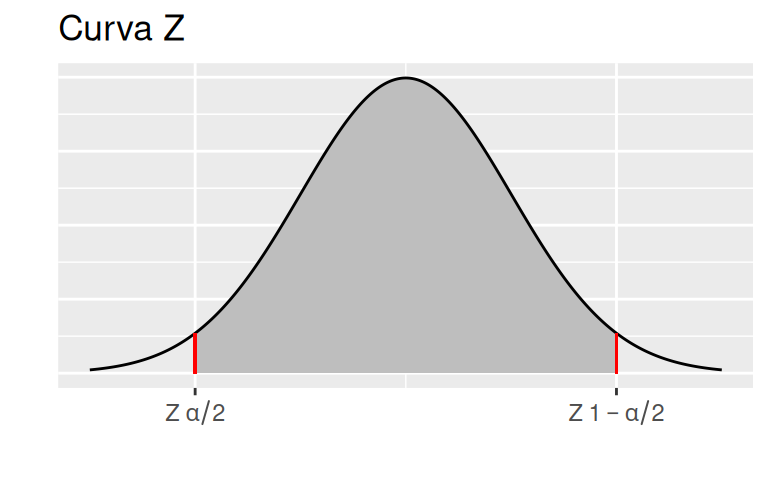
\includegraphics{est2+inferencia_files/figure-latex/normalestandar-1} 

}

\caption{Curva Z, Normal Estándar}\label{fig:normalestandar}
\end{figure}

Luego, reemplazando el valor de \(Z\) por \eqref{eq:normalestandar} en la ecuación \eqref{eq:IC1}, y despejando el valor \(\mu\) al interior de la probabilidad, se obtiene la siguiente expresión.

\begin{equation}
P\left( \bar{X} + Z_{\alpha/2}\frac{\sigma}{\sqrt{n}} < \mu < \bar{X} + Z_{1-\alpha/2}\frac{\sigma}{\sqrt{n}}\right) = 1-\alpha
\label{eq:IntC}
\end{equation}

o

\begin{equation}
P\left( \bar{X} - Z_{1-\alpha/2}\frac{\sigma}{\sqrt{n}} < \mu < \bar{X} + Z_{1-\alpha/2}\frac{\sigma}{\sqrt{n}}\right) = 1-\alpha
\label{eq:IntC2}
\end{equation}

La desigualdad dentro de la probabilidad es el intervalo de confianza construido para la media poblacional, mientras que, el término a la derecha de la igualdad corresponde a la confianza trabajada por el investigador (\(1-\alpha\)).

La siguiente tabla da cuenta de las tipos de intervalo que se pueden elaborar dependiendo del tipo de estimación, es decir, un intervalo bilateral, actoado por la derecha o acotado por la izquierda.

\begin{table}[H]
\centering
\caption{\label{tab:unnamed-chunk-8}Intervalos de confianza para la media de una distribución normal y varianza poblacional conocida}
\centering
\resizebox{\ifdim\width>\linewidth\linewidth\else\width\fi}{!}{
\begin{tabular}[t]{llc}
\toprule
Tipo de intervalo & Probabilidad & Expresión del intervalo\\
\midrule
Bilateral & $P(a < \mu < b) = 1-\alpha$ & $\left(\bar{x} \pm Z_{1-\alpha/2}\displaystyle\frac{\sigma}{\sqrt{n}}\right)$\\
Acotado por la derecha & $P(\mu < b)=1-\alpha$ & $\left( -\infty, \bar{x} + Z_{1-\alpha}\displaystyle\frac{\sigma}{\sqrt{n}}\right)$\\
Acotado por la izquierda & $P(a < \mu)=1-\alpha$ & $\left(\bar{x} - Z_{1-\alpha}\displaystyle\frac{\sigma}{\sqrt{n}}, \infty\right)$\\
\bottomrule
\end{tabular}}
\end{table}

\begin{example}
\protect\hypertarget{exm:ejemplo1IC}{}\label{exm:ejemplo1IC}Los datos que a continuación se dan son los pesos en gramos del contenido de 16 cajas de cereal que se seleccionaron de una proceso de llenado con el propósito de verificar el peso promedio: 506, 508, 499, 503, 504, 510, 497, 512, 514, 505, 493, 496, 506, 502, 509, 496. Si el peso de cada caja es una variable aleatoria normal con una desviación estándar \(\sigma = 5g\), obtener el intervalo de confianza al 99\% para la media de llenado de este proceso.

\emph{Nota}: \(\bar{x} = 503.75\)

Dado que, no se especifica el tipo de intervalo, y que se está interesado es el estudiar la media del llenado de las cajas de cereal, corresponde elaborar un intervalo de confianza bilateral:

\[\left(\bar{x} \pm Z_{1-\alpha/2}\displaystyle\frac{\sigma}{\sqrt{n}}\right)\]

No existe un comando de R (nativo) para elaborar este intervalo, por lo que, la construcción debe ser manual, tal como se muestra a continuación.

\begin{Shaded}
\begin{Highlighting}[]
\NormalTok{peso }\OtherTok{=} \FunctionTok{c}\NormalTok{(}\DecValTok{506}\NormalTok{,}\DecValTok{508}\NormalTok{,}\DecValTok{499}\NormalTok{,}\DecValTok{503}\NormalTok{,}\DecValTok{504}\NormalTok{,}\DecValTok{510}\NormalTok{,}\DecValTok{497}\NormalTok{,}\DecValTok{512}\NormalTok{,}
         \DecValTok{514}\NormalTok{,}\DecValTok{505}\NormalTok{,}\DecValTok{493}\NormalTok{,}\DecValTok{496}\NormalTok{,}\DecValTok{506}\NormalTok{,}\DecValTok{502}\NormalTok{,}\DecValTok{509}\NormalTok{,}\DecValTok{496}\NormalTok{)}
\NormalTok{promedio }\OtherTok{=} \FunctionTok{mean}\NormalTok{(peso)}
\NormalTok{L }\OtherTok{=}\NormalTok{ promedio }\SpecialCharTok{{-}} \FunctionTok{qnorm}\NormalTok{(}\DecValTok{1}\FloatTok{{-}0.01}\SpecialCharTok{/}\DecValTok{2}\NormalTok{)}\SpecialCharTok{*}\DecValTok{5}\SpecialCharTok{/}\FunctionTok{sqrt}\NormalTok{(}\FunctionTok{length}\NormalTok{(peso))}
\NormalTok{U }\OtherTok{=}\NormalTok{ promedio }\SpecialCharTok{+} \FunctionTok{qnorm}\NormalTok{(}\DecValTok{1}\FloatTok{{-}0.01}\SpecialCharTok{/}\DecValTok{2}\NormalTok{)}\SpecialCharTok{*}\DecValTok{5}\SpecialCharTok{/}\FunctionTok{sqrt}\NormalTok{(}\FunctionTok{length}\NormalTok{(peso))}
\FunctionTok{c}\NormalTok{(L,U)}
\end{Highlighting}
\end{Shaded}

\begin{verbatim}
## [1] 500.5302 506.9698
\end{verbatim}

El resultado indica que, la probabilidad de que el intervalo \((500.5, 506.9)\) (en gramos) contenga el valor de la media de llenado de las cajas es de 0.99.
\end{example}

\begin{exercise}
Obtener los intervalos con las confianzas al 90\% y 95\% asociados al ejemplo \ref{exm:ejemplo1IC}. Comente las diferencias e interprete.
\end{exercise}

Dado lo expuesto en el ejercicio anterior, la figura \ref{fig:simulacionIC} muestra la relación que existe entre la confianza y el rango del intervalo, en la cual, es posible observar que a mayor confianza es mayor el rango del intervalo.

\begin{figure}

{\centering 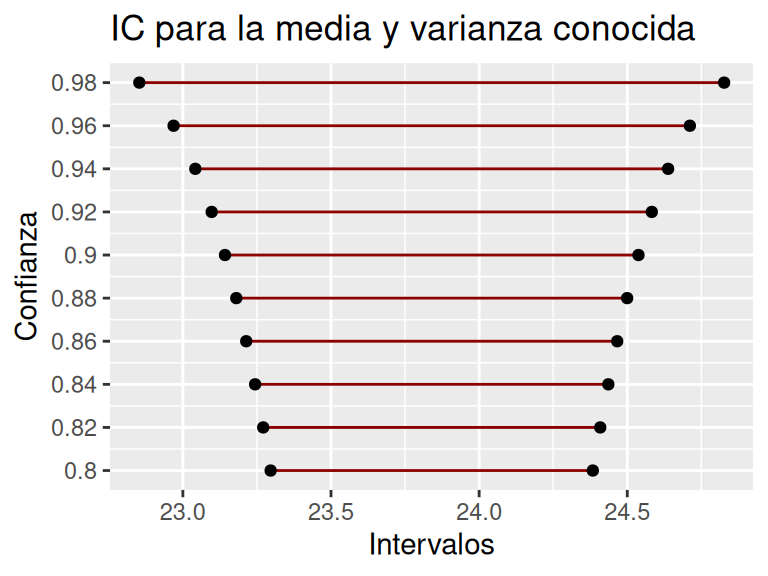
\includegraphics{est2+inferencia_files/figure-latex/simulacionIC-1} 

}

\caption{Simulación de intervalos de confianza para una media con varianza poblacional conocida}\label{fig:simulacionIC}
\end{figure}

Respecto a la interpretación de los intervalos de confianza (en general, y no solo al de esta sección), si la población tiene una distribución normal, el intervalo de confianza que se obtiene con las expresiones (de la tabla anterior) es exacto. En otras palabras, si la expresión se usa repetidas veces para generar intervalos de 95\% de confianza, exactamente 95\% de los intervalos generados contendrán la media poblacional \citep[página 257]{Devore}. El gráfico \ref{fig:sim-ic1} da cuenta del fenómeno para los tres tipos de intervalos de confianza para la media con varianza poblacional desconocida; en cada tipo de intervalo se observa que la cantidad de intervalos que contiene al parámetro (color negro) es cercana a la confianza, lo cual, es más notorio al calcular una mayor cantidad de intervalos.

\begin{figure}

{\centering 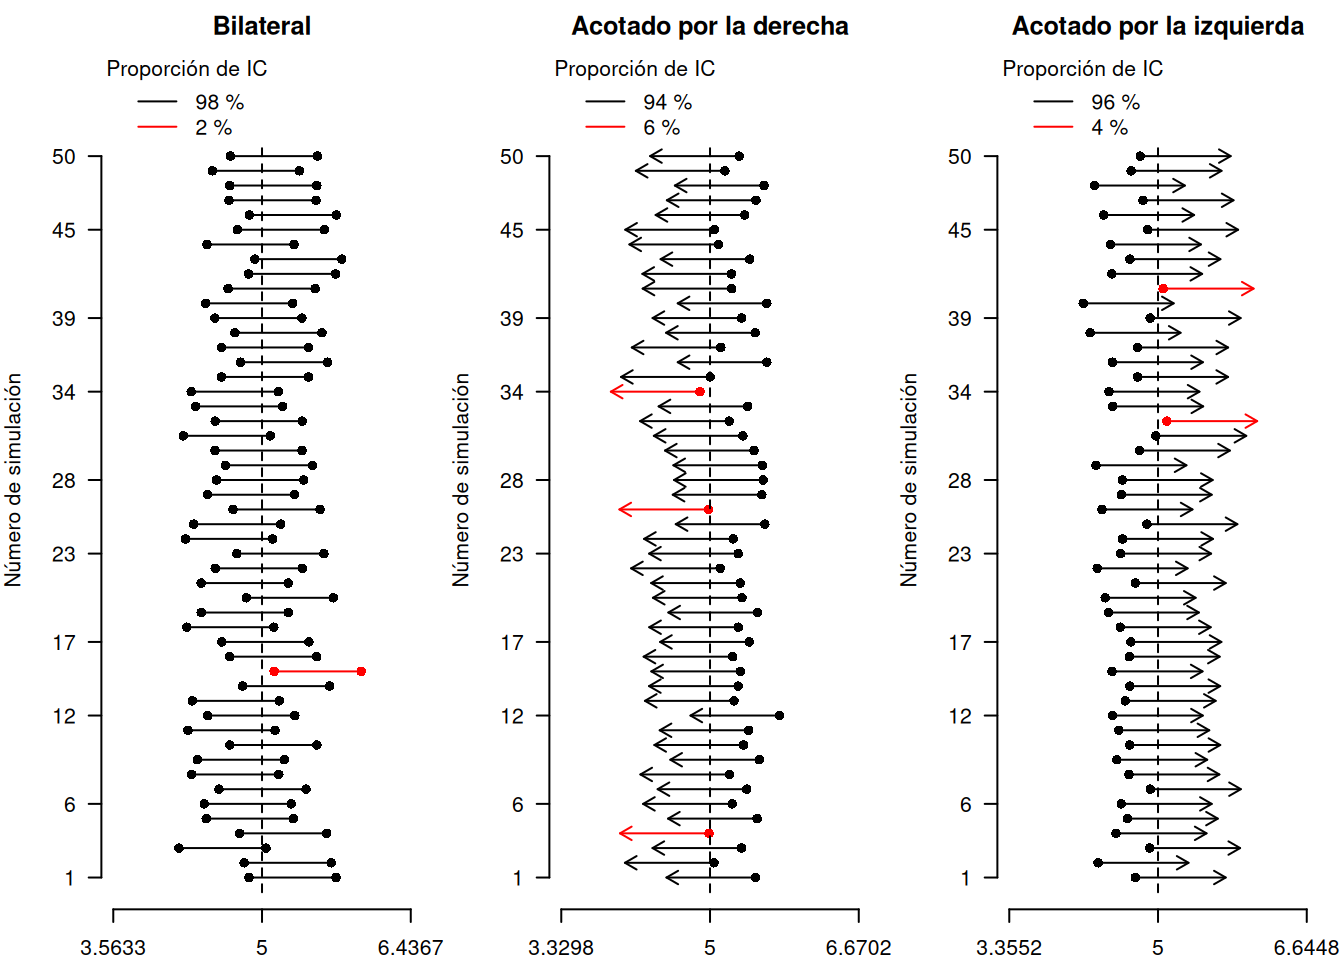
\includegraphics[width=\linewidth]{est2+inferencia_files/figure-latex/sim-ic1-1} 

}

\caption{Simulación de intervalos de confianza para la media con varianza poblacional conocida}\label{fig:sim-ic1}
\end{figure}

\subsection{Varianza poblacional desconocida}\label{intervalo-de-confianza-para-media-varianza-desconocida}

Cuando se calcula un intervalo de confianza para la media poblacional, suele no contarse con una buena estimación de la desviación estándar poblacional. En tales casos se usa la misma muestra para estimar \(\mu\) y \(\sigma\). Esta situación es el caso que se conoce como \(\sigma\) desconocida. Cuando se usa \(S\) para estimar \(\sigma\), el margen de error y la estimación por intervalo de la media poblacional se basan en una distribución de probabilidad conocida como distribución \(t\). \citep[página 307]{anderson}

La razón de que el número de grados de libertad para el valor de \(t\) en la tabla \ref{tab:tabla-ic-una-media-tstudent} sean \(n-1\) se debe al uso de \(S\) como estimación de la desviación estándar poblacional \(\sigma\). La expresión para calcular la desviación estándar muestral es:

\[
S = \sqrt{\frac{1}{n-1}\sum_{i=1}^n (x_i - \bar{x})^2}
\]
Los grados de libertad se refieren al número de valores independientes en el cálculo de \(\sum (x_i - \bar{x})^2\). Los \(n\) valores en el cálculo de \(\sum (x_i - \bar{x})^2\) son los siguientes: \(x_1 - \bar{x},\, x_2 - \bar{x},\, \ldots,\, x_n - \bar{x}\). En estadística 1 se indicó que en cualquier conjunto de datos \(\sum (x_i - \bar{x}) = 0\). Por tanto, únicamente \(n - 1\) de los valores \(x_i - \bar{x}\) son independientes; es decir, si se conocen \(n - 1\) de estos valores, el valor restante puede determinarse exactamente usando el hecho de que los valores \(x_i - \bar{x}\) deben sumar 0. Entonces, \(n - 1\) es el número de grados de libertad en la suma \(\sum (x_i - \bar{x})^2\) y de ahí el número de grados de libertad para la distribución \(t\) en la tabla \ref{tab:tabla-ic-una-media-tstudent}.

\begin{table}[H]
\centering
\caption{\label{tab:tabla-ic-una-media-tstudent}Intervalos de confianza para la media de una distribución normal y varianza poblacional desconocida}
\centering
\resizebox{\ifdim\width>\linewidth\linewidth\else\width\fi}{!}{
\begin{tabular}[t]{llc}
\toprule
Tipo de intervalo & Probabilidad & Expresión del intervalo\\
\midrule
Bilateral & $P(a < \mu < b) = 1-\alpha$ & $\left(\bar{x} \pm t_{1-\alpha/2,n-1}\displaystyle\frac{S}{\sqrt{n}} \right)$\\
Acotado por la derecha & $P(\mu < b)=1-\alpha$ & $\left( -\infty, \bar{x} + t_{1-\alpha,n-1}\displaystyle\frac{S}{\sqrt{n}}\right)$\\
Acotado por la izquierda & $P(a < \mu)=1-\alpha$ & $\left(\bar{x} - t_{1-\alpha,n-1}\displaystyle\frac{S}{\sqrt{n}}, \infty\right)$\\
\bottomrule
\end{tabular}}
\end{table}

\begin{example}
Para resolver el ejemplo \ref{exm:ejemplo1IC} considerando varianza poblacional desconocida, es posible utilizar el comando \texttt{t.test()} para obtener el intervalo de confianza.

\[\left(\bar{x} \pm t_{1-\alpha/2,n-1}\displaystyle\frac{S}{\sqrt{n}} \right)\]

\begin{Shaded}
\begin{Highlighting}[]
\NormalTok{peso }\OtherTok{=} \FunctionTok{c}\NormalTok{(}\DecValTok{506}\NormalTok{,}\DecValTok{508}\NormalTok{,}\DecValTok{499}\NormalTok{,}\DecValTok{503}\NormalTok{,}\DecValTok{504}\NormalTok{,}\DecValTok{510}\NormalTok{,}\DecValTok{497}\NormalTok{,}\DecValTok{512}\NormalTok{,}
         \DecValTok{514}\NormalTok{,}\DecValTok{505}\NormalTok{,}\DecValTok{493}\NormalTok{,}\DecValTok{496}\NormalTok{,}\DecValTok{506}\NormalTok{,}\DecValTok{502}\NormalTok{,}\DecValTok{509}\NormalTok{,}\DecValTok{496}\NormalTok{)}
\FunctionTok{t.test}\NormalTok{(}\AttributeTok{x =}\NormalTok{ peso, }\AttributeTok{conf.level =} \FloatTok{0.99}\NormalTok{, }\AttributeTok{alternative =} \StringTok{"two.sided"}\NormalTok{)}
\end{Highlighting}
\end{Shaded}

\begin{verbatim}
## 
##  One Sample t-test
## 
## data:  peso
## t = 324.89, df = 15, p-value < 2.2e-16
## alternative hypothesis: true mean is not equal to 0
## 99 percent confidence interval:
##  499.181 508.319
## sample estimates:
## mean of x 
##    503.75
\end{verbatim}

En este sentido, se tiene una probabilidad de 0.99 de que el intervalo \((499.1, 508.3)\) contenga el valor de la media de llenado de las cajas de cereal.
\end{example}

\begin{exercise}

Utilizando la base de datos del \hyperref[Imacec1]{Imacec}:

\begin{enumerate}
\def\labelenumi{\arabic{enumi}.}
\tightlist
\item
  Elabore un intervalo de confianza para estudiar el valor promedio del Imacec en el sector de Minería en los años 2019 y 2021, asumiendo que el Imacec de Minería es una variable aleatoria que distribuye normal. Utilice una confianza de 91\%. Interprete.
\item
  Elabore un intervalo de confianza para estudiar si, el valor promedio del Imacec en el sector de Industria en los años 2019 y 2021 es mayor a 100, asumiendo que el Imacec de Industria es una variable aleatoria que distribuye normal. Utilice una confianza de 91\%. Interprete.
\end{enumerate}

\end{exercise}

\section{Intervalo de confianza para la diferencia de medias}\label{intervalo-de-confianza-para-la-diferencia-de-medias}

\subsection{Varianzas poblacionales conocidas}\label{intervalo-de-confianza-para-la-diferencia-de-medias-varianzas-conocidas}

Sean \(\mu_X\) la media de la población X y \(\mu_Y\) la media de la población Y, lo que interesa aquí son inferencias acerca de la diferencia entre las medias: \(\mu_X - \mu_Y\). Para hacer una inferencia acerca de esta diferencia, se elige una muestra aleatoria simple de \(n_X\) unidades de la población X y otra muestra aleatoria simple de \(n_Y\) unidades de la población Y. A estas dos muestras que se toman separada e independientemente se les conoce como muestras aleatorias simples independientes.

Si ambas poblaciones tienen distribución normal o si los tamaños de las muestras son suficientemente grandes para que el teorema del límite central permita concluir
que las distribuciones muestrales de \(\bar{X}\) y \(\bar{Y}\) puedan ser aproximadas mediante una distribución normal, la distribución muestral de \(\bar{X} - \bar{Y}\) tendrá una distribución normal.

En esta sección se supondrá que se cuenta con información que permite considerar que las dos desviaciones estándar \(\sigma_X\) y \(\sigma_Y\) se conocen antes de tomar las muestras. Este caso se conoce como el caso de varianzas conocidas. \citep[página 396]{anderson}

\begin{table}[H]
\centering
\caption{\label{tab:unnamed-chunk-11}Intervalos de confianza para la diferencia de medias de dos distribucones normales y varianzas poblacionales conocidas}
\centering
\resizebox{\ifdim\width>\linewidth\linewidth\else\width\fi}{!}{
\begin{tabular}[t]{llc}
\toprule
Tipo de intervalo & Probabilidad & Expresión del intervalo\\
\midrule
Bilateral & $P(a < \mu_X - \mu_Y < b) = 1-\alpha$ & $\left(\bar{x} - \bar{y} \pm Z_{1-\alpha/2}\displaystyle\sqrt{\displaystyle\frac{\sigma^2_X}{n_x} + \displaystyle\frac{\sigma^2_Y}{n_y}}\right)$\\
Acotado por la derecha & $P(\mu_X - \mu_Y < b) = 1-\alpha$ & $\left( -\infty, \bar{x} - \bar{y} + Z_{1-\alpha}\displaystyle\sqrt{\displaystyle\frac{\sigma^2_X}{n_x} + \displaystyle\frac{\sigma^2_Y}{n_y}}\right)$\\
Acotado por la izquierda & $P(a < \mu_X - \mu_Y) = 1-\alpha$ & $\left(\bar{x} - \bar{y} - Z_{1-\alpha}\displaystyle\sqrt{\displaystyle\frac{\sigma^2_X}{n_x} + \displaystyle\frac{\sigma^2_Y}{n_y}}, \infty\right)$\\
\bottomrule
\end{tabular}}
\end{table}

\begin{example}
\protect\hypertarget{exm:ICdiferencianormal}{}\label{exm:ICdiferencianormal}La base de datos \href{https://raw.githubusercontent.com/Dfranzani/Bases-de-datos-para-cursos/main/2022-2/Estad\%C3\%ADstica\%201/dolar.csv}{dolar.csv} contiene los datos asociados al tipo de cambio del dólar. Las columnas de la base de datos son las siguientes:

\begin{itemize}
\tightlist
\item
  Mes: mes de medición.
\item
  Dia: día de medición.
\item
  Valor: tipo de cambio del dólar a pesos (clp).
\end{itemize}

Elabore un intervalo de confianza para estudiar la diferencia del valor promedio del dólar entre los meses de junio y julio, asumiendo distribución normal de los datos en ambas poblaciones, y varianzas poblacionales de 1250 y 580 para cada mes respectivamente. Utilice una confianza del 95\%.

Al conocer las varianzas poblacionales, y querer estudiar la diferencia, corresponde elaborar el siguiente intervalo de confianza.

\[\left(\bar{x} - \bar{y} \pm Z_{1-\alpha/2}\displaystyle\sqrt{\displaystyle\frac{\sigma^2_X}{n_x} + \displaystyle\frac{\sigma^2_Y}{n_y}}\right)\]
No existe un comando en R que permita generar este intervalo de confianza, por lo que corresponde construirlo manualmente, tal como se muestra a continuación.

\begin{Shaded}
\begin{Highlighting}[]
\CommentTok{\# Cargue previamente la base datos, guardándola con el nombre "df"}
\NormalTok{junio }\OtherTok{=}\NormalTok{ df}\SpecialCharTok{$}\NormalTok{Valor[df}\SpecialCharTok{$}\NormalTok{Mes}\SpecialCharTok{==}\StringTok{"Junio"}\NormalTok{]}
\NormalTok{julio }\OtherTok{=}\NormalTok{ df}\SpecialCharTok{$}\NormalTok{Valor[df}\SpecialCharTok{$}\NormalTok{Mes}\SpecialCharTok{==}\StringTok{"Julio"}\NormalTok{]}
\NormalTok{L }\OtherTok{=} \FunctionTok{mean}\NormalTok{(junio) }\SpecialCharTok{{-}} \FunctionTok{mean}\NormalTok{(julio) }\SpecialCharTok{{-}} 
  \FunctionTok{qnorm}\NormalTok{(}\DecValTok{1}\FloatTok{{-}0.05}\SpecialCharTok{/}\DecValTok{2}\NormalTok{)}\SpecialCharTok{*}
  \FunctionTok{sqrt}\NormalTok{(}\DecValTok{1250}\SpecialCharTok{/}\FunctionTok{length}\NormalTok{(junio) }\SpecialCharTok{+} \DecValTok{580}\SpecialCharTok{/}\FunctionTok{length}\NormalTok{(julio))}
\NormalTok{U }\OtherTok{=} \FunctionTok{mean}\NormalTok{(junio) }\SpecialCharTok{{-}} \FunctionTok{mean}\NormalTok{(julio) }\SpecialCharTok{+} 
  \FunctionTok{qnorm}\NormalTok{(}\DecValTok{1}\FloatTok{{-}0.05}\SpecialCharTok{/}\DecValTok{2}\NormalTok{)}\SpecialCharTok{*}
  \FunctionTok{sqrt}\NormalTok{(}\DecValTok{1250}\SpecialCharTok{/}\FunctionTok{length}\NormalTok{(junio) }\SpecialCharTok{+} \DecValTok{580}\SpecialCharTok{/}\FunctionTok{length}\NormalTok{(julio))}
\FunctionTok{c}\NormalTok{(L,U)}
\end{Highlighting}
\end{Shaded}

\begin{verbatim}
## [1] -103.85536  -65.70453
\end{verbatim}

El resultado indica que, la probabilidad de que el intervalo \((-103.8,  -65.7)\) (en pesos) contenga al valor real de la diferencia entre ambas medias es de 0.95.
\end{example}

\begin{exercise}
Estudiar si el valor promedio del dólar de Julio es mayor al de Junio por más de 50 pesos (clp). Considere que las variables distribuyen normal, y que las varianzas poblacionales son las mismas que se mencionan en el ejemplo \ref{exm:ICdiferencianormal}. Utilice una confianza del 92.3\%. Interprete.
\end{exercise}

\subsection{Varianzas poblacionales desconocidas e iguales}\label{intervalo-de-confianza-para-la-diferencia-de-medias-varianzas-desconocidas-iguales}

En esta sección el estudio de las inferencias sobre la diferencia entre dos medias poblacionales se extiende al caso en el que las dos desviaciones estándar poblacionales, \(\sigma_X\) y \(\sigma_Y\) no se conocen, además de considerar de que son iguales. En este caso, para estimar las desviaciones estándar poblacionales desconocidas se emplean las desviaciones estándar muestrales, \(S_X\) y \(S_Y\). Cuando se usan las desviaciones estándar muestrales en las estimaciones por intervalo y en las pruebas de hipótesis, se emplea la distribución \(t\) en lugar de la distribución normal estándar.

\begin{table}[H]
\centering
\caption{\label{tab:unnamed-chunk-14}Intervalos de confianza para la diferencia de medias de dos distribucones normales y varianzas poblacionales desconocidas e iguales}
\centering
\resizebox{\ifdim\width>\linewidth\linewidth\else\width\fi}{!}{
\begin{tabular}[t]{llc}
\toprule
Tipo de intervalo & Probabilidad & Expresión del intervalo\\
\midrule
Bilateral & $P(a < \mu_X - \mu_Y < b) = 1-\alpha$ & $\left(\bar{x} - \bar{y} \pm t_{1-\alpha/2,k}S_p\displaystyle\sqrt{\displaystyle\frac{1}{n_x} + \displaystyle\frac{1}{n_y}}\right)$\\
Acotado por la derecha & $P(\mu_X - \mu_Y < b) = 1-\alpha$ & $\left( -\infty, \bar{x} - \bar{y} + t_{1-\alpha,k}S_p\displaystyle\sqrt{\displaystyle\frac{1}{n_x} + \displaystyle\frac{1}{n_y}}\right)$\\
Acotado por la izquierda & $P(a < \mu_X - \mu_Y) = 1-\alpha$ & $\left(\bar{x} - \bar{y} - t_{1-\alpha,k}S_p\displaystyle\sqrt{\displaystyle\frac{1}{n_x} + \displaystyle\frac{1}{n_y}}, \infty\right)$\\
\bottomrule
\end{tabular}}
\end{table}

donde,

\[k = n_X + n_Y-2\]

\[S_p^2 = \frac{(n_X-1)S_X^2 + (n_Y-1)S_Y^2}{n_X+n_Y-2}\]

\begin{example}
\protect\hypertarget{exm:ejemploICdiferencia}{}\label{exm:ejemploICdiferencia}Dos universidades financiadas por el gobierno tienen métodos distintos para inscribir a sus alumnos a principios de cada semestre. Las dos desean comparar el tiempo promedio que les toma a los estudiantes el trámite de inscripción. En cada universidad se anotaron los tiempo de inscripción para 30 alumnos seleccionados al azar. Las medias y las desviaciones estándar muestrales son las siguientes:

\begin{equation}
\notag
\begin{matrix}
\bar{x}_1 = 50.2 & \bar{x}_2=52.9\\
S_1 = 4.8 & S_2 = 5.4
\end{matrix}
\end{equation}

Si se supone que el muestreo se llevó a cabo sobre dos poblaciones distribuidas normales e independientes con varianzas iguales , obtener el intervalo de confianza estimado del 99\% para la diferencia entre las medias del tiempo de inscripción para las dos universidades. Con base en este evidencia, ¿se estaría inclinando a concluir que existe una diferencia real entre los tiempos medios para cada universidad?

Para responder a la pregunta, es necesario construir un intervalo de confianza para la diferencia de medias y, verificar si el cero está incluido dentro de este. El desarrollo del intervalo debe ser manual, ya que, no se cuenta con una base de datos, sino que directamente con los promedios y desviaciones estándar de las muestras.

\begin{equation}
\notag
\begin{split}
&\left(\bar{x}_1 - \bar{x}_2 \pm t_{1-\alpha/2,k}S_p\displaystyle\sqrt{\displaystyle\frac{1}{n_{X_1}} + \displaystyle\frac{1}{n_{X_2}}}\right) = \left(-6.208;0.808 \right)\\
S_p^2 &= \frac{(n_{X_1}-1)S_{X_1}^2 + (n_{X_2}-1)S_{X_2}^2}{n_{X_1}+n_{X_2}-2} = \frac{29\cdot 4.8^2 + 29\cdot 5.4^2}{58} = 26.1\\
k &= n_{X_1} + n_{X_2}-2 = 58 \text{, } t_{0.995, 58} = 2.66\\
\end{split}
\end{equation}

Como el intervalo contiene al cero, no existe suficiente evidencia para indicar que existe una diferencia real entre los tiempos medios para cada universidad, con un 99\% de confianza.
\end{example}

\begin{exercise}
\protect\hypertarget{exr:ICcontrolcuotas}{}\label{exr:ICcontrolcuotas}La base de datos \hyperref[Cuotas]{Control cuotas} contiene los datos de los valores cuota de los primeros tres meses del año 2022 de las AFP Plan Vital y Provida. Se está interesado en saber si el valor promedio de las cuotas de Plan Vital supera al de Provida por más de 30000 pesos, para ello, elabore un intervalo de confianza con una confianza del 90\%. Asuma, que el valor cuota es una variable aleatoria que distribuye normal en ambas poblaciones (independientes), y que las varianzas poblacionales son desconocidas e iguales.
\end{exercise}

\begin{exercise}
Utilizando la base de datos \hyperref[Cuotas]{Control cuotas}, estudiar si la media del valor cuota de Provida es menor a la de Plan Vital, utilizando una confianza del 99.64\% Considere distribución normal de las variables y varianzas poblacionales desconocidas e iguales.
\end{exercise}

\subsection{Varianzas poblacionales desconocidas y distintas}\label{intervalo-de-confianza-para-la-diferencia-de-medias-varianzas-desconocidas-distintas}

A diferencia de los visto en la sección anterior, las dos desviaciones estándar poblacionales, \(\sigma_X\) y \(\sigma_Y\) si bien no se conocen, se consideran distintas.

\begin{table}[H]
\centering
\caption{\label{tab:unnamed-chunk-15}Intervalos de confianza para la diferencia de medias de dos distribucones normales y varianzas poblacionales desconocidas y distintas}
\centering
\resizebox{\ifdim\width>\linewidth\linewidth\else\width\fi}{!}{
\begin{tabular}[t]{llc}
\toprule
Tipo de intervalo & Probabilidad & Expresión del intervalo\\
\midrule
Bilateral & $P(a < \mu_X - \mu_Y < b) = 1-\alpha$ & $\left(\bar{x} - \bar{y} \pm t_{1-\alpha/2,k}\sqrt{S^2_X/n_X + S^2_Y/n_Y}\right)$\\
Acotado por la derecha & $P(\mu_X - \mu_Y < b) = 1-\alpha$ & $\left( -\infty, \bar{x} - \bar{y} + t_{1-\alpha,k}\sqrt{S^2_X/n_X + S^2_Y/n_Y}\right)$\\
Acotado por la izquierda & $P(a < \mu_X - \mu_Y) = 1-\alpha$ & $\left(\bar{x} - \bar{y} - t_{1-\alpha,k}\sqrt{S^2_X/n_X + S^2_Y/n_Y}, \infty\right)$\\
\bottomrule
\end{tabular}}
\end{table}

dónde \(k\) es el entero más cercano a

\[\frac{(S_X^2/n_X + S_Y^2/n_Y)^2}{(S_X^2/n_X)^2/(n_X-1) + (S_Y^2/n_Y)^2/(n_Y-1)}\]

\begin{example}
Resuelva el ejemplo \ref{exm:ICdiferencianormal} asumiendo varianzas poblacionales desconocidas y diferentes.

Al asumir que las varianzas poblacionales son desconocidas y diferentes, corresponde elaborar el siguiente intervalo.

\[\left(\bar{x} - \bar{y} \pm t_{1-\alpha/2,k}\sqrt{S^2_X/n_X + S^2_Y/n_Y}\right)\]

La ejecución en R es mediante el comando \texttt{t.test()} considerando el argumento \texttt{var.equal\ =\ F}, el cual, indica que las varianzas poblacionales son desconocidas y distintas (por defecto el valor de este argumento es \texttt{F}, es decir, se asume que las varianzas poblacionales son desconocidas y distintas). Además, se asume una confianza del 95\%.

\begin{Shaded}
\begin{Highlighting}[]
\NormalTok{junio }\OtherTok{=}\NormalTok{ df}\SpecialCharTok{$}\NormalTok{Valor[df}\SpecialCharTok{$}\NormalTok{Mes}\SpecialCharTok{==}\StringTok{"Junio"}\NormalTok{]}
\NormalTok{julio }\OtherTok{=}\NormalTok{ df}\SpecialCharTok{$}\NormalTok{Valor[df}\SpecialCharTok{$}\NormalTok{Mes}\SpecialCharTok{==}\StringTok{"Julio"}\NormalTok{]}
\FunctionTok{t.test}\NormalTok{(}\AttributeTok{x =}\NormalTok{ junio, }\AttributeTok{y =}\NormalTok{ julio, }\AttributeTok{conf.level =} \FloatTok{0.95}\NormalTok{, }\AttributeTok{var.equal =}\NormalTok{ F)}
\end{Highlighting}
\end{Shaded}

\begin{verbatim}
## 
##  Welch Two Sample t-test
## 
## data:  junio and julio
## t = -8.793, df = 33.349, p-value = 3.338e-10
## alternative hypothesis: true difference in means is not equal to 0
## 95 percent confidence interval:
##  -104.38837  -65.17152
## sample estimates:
## mean of x mean of y 
##  857.7695  942.5494
\end{verbatim}

El resultado indica que, la probabilidad de que el intervalo \((-104.3,  -65.17)\) (en pesos) contenga al valor real de la diferencia entre ambas medias es de 0.95.
\end{example}

\begin{exercise}
Utilizando la base de datos del \hyperref[Imacec1]{Imacec}, elabore un intervalo de confianza para estudiar si, la media del Imacec del sector de minería es menor al del sector de industria en el periodo 2019-2020. Asuma que, las distribuciones poblacionales son normales e indendientes, y que las varianzas poblacionales son desconocidas y distintas. Utilice una confianza del 96\%. Interprete.
\end{exercise}

\section{Intervalo de confianza para la comparación de varianzas}\label{intervalo-de-confianza-comparacion-de-varianzas}

De vez en cuando se requieren métodos de comparar dos varianzas de población (o desviaciones estándar), aunque tales problemas surgen con mucho menor frecuencia que aquellos que implican medias o proporciones. Para el caso en que las poblaciones investigadas son normales, los procedimientos están basados en una nueva familia de distribuciones de probabilidad.

\subsection*{Distribución F}\label{distribucion-f}
\addcontentsline{toc}{subsection}{Distribución F}

La distribución de probabilidad \(F\) tiene dos parámetros, denotados por \(\nu_{1}\) y \(\nu_{2}\). El parámetro \(\nu_{1}\) se conoce como \textit{numerador de número de grados de libertad} y \(\nu_{2}\) es el \textit{denominador de número de grados de libertad}; en este caso \(\nu_{1}\) y \(\nu_{2}\) son enteros positivos. Una variable aleatoria que tiene una distribución \(F\) no puede asumir un valor negativo. Como la función de densidad es complicada y no será utilizada en forma explícita, se omite la fórmula. Existe una importante conexión entre una variable \(F\) y variables chi-cuadrado. Si \(X_{1}\) y \(X_{2}\) son variables aleatorias chi-cuadradas independientes con \(\nu_{1}\) y \(\nu_{2}\) grados de libertad, respectivamente, entonces la variable aleatoria

\[
F = \frac{X_{1}/\nu_{1}}{X_{2}/\nu_{2}}
\]

se puede demostrar que la razón de las dos variables chi-cuadradas divididas entre sus respectivos grados de libertad tiene una distribución \(F\). \citep[página 360]{Devore}

En esta sección, se hará uso únicamente del intervalo bilateral, ya que, es el único tipo de intervalo que no permite determinar si las varianzas poblacionales deben ser consideradas desconocidas distintas o iguales.

\begin{equation}
\begin{split}
P\left(a<\frac{\sigma_Y^2}{\sigma_X^2}<b\right) = 1-\alpha &\Rightarrow \left( F_1\frac{S_Y^2}{S_X^2},F_2\frac{S_Y^2}{S_X^2} \right)\\
& F_1 = \frac{1}{f_{1-\alpha/2,n_Y-1,n_X-1}}\\
& F_2 = f_{1-\alpha/2,n_X-1,n_Y-1}
\end{split}
\label{eq:ICvarianzas-bilateral}
\end{equation}

\begin{example}
Utilizando la base de datos \href{https://raw.githubusercontent.com/Dfranzani/Bases-de-datos-para-cursos/main/2022-2/Estad\%C3\%ADstica\%201/dolar.csv}{dolar.csv}, elabore un intervalo de confianza para el cociente de la variabilidad del valor del dólar entre los meses de junio y julio, asumiendo que las distribuciones poblacionales son normales e independientes

Para estudiar o comparar varianzas, corresponde elaborar el único intervalo especificado en esta sección.

\[\left( F_1\frac{S_Y^2}{S_X^2},F_2\frac{S_Y^2}{S_X^2} \right)\]

La ejecución en R, considerando una confianza del 95\% es la siguiente.

\begin{Shaded}
\begin{Highlighting}[]
\NormalTok{junio }\OtherTok{=}\NormalTok{ df}\SpecialCharTok{$}\NormalTok{Valor[df}\SpecialCharTok{$}\NormalTok{Mes}\SpecialCharTok{==}\StringTok{"Junio"}\NormalTok{]}
\NormalTok{julio }\OtherTok{=}\NormalTok{ df}\SpecialCharTok{$}\NormalTok{Valor[df}\SpecialCharTok{$}\NormalTok{Mes}\SpecialCharTok{==}\StringTok{"Julio"}\NormalTok{]}
\FunctionTok{var.test}\NormalTok{(}\AttributeTok{x =}\NormalTok{ junio, }\AttributeTok{y =}\NormalTok{ julio, }\AttributeTok{conf.level =} \FloatTok{0.95}\NormalTok{)}
\end{Highlighting}
\end{Shaded}

\begin{verbatim}
## 
##  F test to compare two variances
## 
## data:  junio and julio
## F = 2.2409, num df = 19, denom df = 17, p-value = 0.1004
## alternative hypothesis: true ratio of variances is not equal to 1
## 95 percent confidence interval:
##  0.8510277 5.7522904
## sample estimates:
## ratio of variances 
##           2.240867
\end{verbatim}

Dado que, la probabilidad asociada a este intervalo de confianza contiene al cociente de las varianzas poblacionales, para determinar si existe o no diferencia entre estos parámetros se debe verificar si el 1 está dentro o no del intervalo. En caso de que el 1 esté dentro del intervalo, entonces, se asume que las varianzas poblacionales son iguales.

En este sentido, el intervalo asociado al ejemplo es \((0.8, 5.7)\), el cual, contiene al 1. Por lo tanto, se asume que las varianzas del valor del dólar de ambos meses es igual, con un 95\% de confianza.
\end{example}

\begin{exercise}
Considerando el ejercicio \ref{exr:ICcontrolcuotas}, elabore un intervalo de confianza para la comparación de varianzas de ambas poblaciones. Asuma, que las distribuciones poblacionales son normales e independientes. Utilice una confianza del 93.2\%. Interprete.
\end{exercise}

\begin{exercise}
Utilizando la base de datos del \hyperref[Imacec1]{Imacec}, elabore un intervalo de confianza para comparar la variabilidad (varianza) del valor del Imacec entre ambos sectores. Asuma, que las distribuciones poblacionales son normales e independientes. Utilice una confianza del 90\%. Interprete.
\end{exercise}

\begin{exercise}
Utilizando la base de datos del \hyperref[Imacec1]{Imacec}, elabore un intervalo de confianza para estudiar la diferencia la media del Imacec de ambos sectores. Asuma, que las distribuciones poblacionales son normales e independientes. Utilice una confianza del 92\%. Interprete.
\end{exercise}

\begin{exercise}
Utilizando la base de datos del \hyperref[Imacec1]{Imacec}, elabore un intervalo de confianza para estudiar si, el promedio del Imacec de minería es mayor al de industria por más de 2 unidades. Asuma, que las distribuciones poblacionales son normales e independientes. Utilice una confianza del 97\%. Interprete.
\end{exercise}

\section{Ejercicios}\label{ejercicios-unidad1}

A continuación, desarrolle los ejercicios manualmente sin el uso de R.

\begin{exercise}
Una empresa desea estimar el tiempo promedio de espera (en minutos) en un sistema de atención. Se sabe que la desviación estándar poblacional es \(\sigma = 2.0\) minutos. Se registraron los siguientes tiempos de espera: 18, 20, 17, 22, 19, 21, 20, 18, 19, 20. Con un nivel de confianza del 95\% y asumiendo normalidad de los datos, elabore un intervalo de confianza para estudiar el promedio poblacional de los tiempos de espera. Use que \(Z_{1-0.05/2} = 1.9599\). En su respuesta indique la media poblacional en estudio, el tipo de intervalo, el nivel de confianza utilizado y la interpretación en el contexto.
\end{exercise}

\begin{exercise}
Un investigador mide la satisfacción de clientes en una escala de 0 a 100 puntos. La varianza poblacional es desconocida. Se registraron los siguientes valores: 72, 75, 78, 70, 74, 80, 77, 73. Con un nivel de confianza del 99\% y asumiendo normalidad de los datos, elabore un intervalo de confianza para estudiar si el promedio poblacional supera 75. Use que \(t_{1-0.01,\,7} = 2.9980\). En su respuesta indique la media poblacional en estudio, el tipo de intervalo, el nivel de confianza utilizado y la interpretación en el contexto.
\end{exercise}

\begin{exercise}
Dos métodos de producción (A y B) generan rendimientos (en unidades por hora). Se conocen las desviaciones estándar poblacionales: \(\sigma_A = 3.0\) y \(\sigma_B = 2.5\). Para el método A se obtuvieron los siguientes datos: 102, 100, 98, 101, 99, 100, 97, 103, 101, 98. Para el método B se obtuvieron los siguientes datos: 95, 97, 94, 96, 95, 93, 92, 94, 96. Con un nivel de confianza del 90\% y asumiendo normalidad de los datos, elabore un intervalo de confianza para estudiar si la media poblacional de A es mayor que la de B por menos de 6 unidades. Use que \(Z_{0.10} = 1.2816\). En su respuesta indique las medias poblacionales en estudio, el tipo de intervalo, el nivel de confianza utilizado y la interpretación en el contexto.
\end{exercise}

\begin{exercise}
Un equipo desea estimar el tiempo promedio (en minutos) de descarga de un archivo. Se conoce la desviación estándar poblacional \(\sigma = 1.5\). Se registraron los siguientes tiempos: 5.2, 4.8, 5.5, 5.1, 4.9, 5.3, 5.0, 5.4, 4.7, 5.2. Con un nivel de confianza del 99\% y asumiendo normalidad de los datos, elabore un intervalo de confianza para estudiar el promedio poblacional de los tiempos de descarga. Use que \(Z_{1-0.01/2} = 2.5758\). En su respuesta indique la media poblacional en estudio, el tipo de intervalo, el nivel de confianza utilizado y la interpretación en el contexto.
\end{exercise}

\begin{exercise}
Una empresa monitorea el gasto promedio por compra (en miles de pesos). La varianza poblacional es desconocida. Se registraron los siguientes montos: 62, 68, 71, 65, 69, 70, 66, 64, 67. Con un nivel de confianza del 95\% y asumiendo normalidad de los datos, elabore un intervalo de confianza para estudiar si el gasto promedio poblacional es menor a 70. Use que \(t_{1-0.05,\,8} = 1.8331\). En su respuesta indique la media poblacional en estudio, el tipo de intervalo, el nivel de confianza utilizado y la interpretación en el contexto.
\end{exercise}

\begin{exercise}
Dos líneas de producción (A y B) registran rendimiento (unidades por hora). Se conocen las desviaciones estándar poblacionales: \(\sigma_A = 2.0\) y \(\sigma_B = 2.2\). Para A se observaron los siguientes valores: 48, 50, 49, 51, 52, 47, 50, 49, 51. Para B se observaron los siguientes valores: 45, 46, 47, 44, 46, 45, 47, 48. Con un nivel de confianza del 97\% y asumiendo normalidad de los datos, elabore un intervalo de confianza para estudiar si el rendimiento promedio de A supera al de B por más de 3 unidades. Use que \(Z_{0.97} = 1.8808\). En su respuesta indique las medias poblacionales en estudio, el tipo de intervalo, el nivel de confianza utilizado y la interpretación en el contexto.
\end{exercise}

\begin{exercise}
Un servicio técnico registra la duración (en minutos) de reparaciones rápidas. Se conoce la desviación estándar poblacional \(\sigma = 3.0\). Se observaron los valores: 34, 29, 31, 33, 35, 30, 28, 32, 31, 34, 30. Con un nivel de confianza del 90\% y asumiendo normalidad de los datos, elabore un intervalo de confianza para estudiar el promedio poblacional de la duración de las reparaciones. Use que \(Z_{0.95} = 1.6449\). En su respuesta indique la media poblacional en estudio, el tipo de intervalo, el nivel de confianza utilizado y la interpretación en el contexto.
\end{exercise}

\begin{exercise}
En una encuesta de satisfacción (0--100), la varianza poblacional es desconocida. Se registraron los siguientes puntajes: 81, 79, 85, 83, 80, 78, 82, 84, 81, 77. Con un nivel de confianza del 98\% y asumiendo normalidad de los datos, elabore un intervalo de confianza para estudiar si el promedio poblacional supera 80. Use que \(t_{1-0.02,\,9} = 2.2622\). En su respuesta indique la media poblacional en estudio, el tipo de intervalo, el nivel de confianza utilizado y la interpretación en el contexto.
\end{exercise}

\begin{exercise}
Dos aplicaciones (A y B) miden el tiempo de respuesta (en milisegundos). Se conocen las desviaciones estándar poblacionales: \(\sigma_A = 12\) y \(\sigma_B = 10\). Para A se observaron: 210, 205, 198, 202, 207, 200, 203, 206, 199. Para B se observaron: 195, 197, 193, 198, 196, 194, 199, 192. Con un nivel de confianza del 95\% y asumiendo normalidad de los datos, elabore un intervalo de confianza para estudiar si el tiempo promedio de A es menor que el de B por menos de 8 ms. Use que \(Z_{0.95} = 1.6449\). En su respuesta indique las medias poblacionales en estudio, el tipo de intervalo, el nivel de confianza utilizado y la interpretación en el contexto.
\end{exercise}

\begin{exercise}
Una fintech registra el tiempo de aprobación de solicitudes (segundos). Se conoce la desviación estándar poblacional \(\sigma = 4.0\). Se observaron los valores: 52, 48, 50, 55, 53, 49, 51, 47, 54, 50. Con un nivel de confianza del 92\% y asumiendo normalidad de los datos, elabore un intervalo de confianza para estudiar el promedio poblacional del tiempo de aprobación. Use que \(Z_{0.96} = 1.7507\). En su respuesta indique la media poblacional en estudio, el tipo de intervalo, el nivel de confianza utilizado y la interpretación en el contexto.
\end{exercise}

\begin{exercise}
Un banco evalúa el tiempo promedio de atención (minutos) y la varianza poblacional es desconocida. Se registraron los tiempos: 9.2, 10.1, 8.7, 9.5, 9.8, 10.3, 9.0, 9.6. Con un nivel de confianza del 90\% y asumiendo normalidad de los datos, elabore un intervalo de confianza para estudiar si el tiempo promedio poblacional es menor a 10. Use que \(t_{1-0.10,\,7} = 1.4398\). En su respuesta indique la media poblacional en estudio, el tipo de intervalo, el nivel de confianza utilizado y la interpretación en el contexto.
\end{exercise}

\begin{exercise}
Dos campañas (A y B) reportan la tasa de clics (por mil impresiones). Se conocen las desviaciones estándar poblacionales: \(\sigma_A = 0.9\) y \(\sigma_B = 1.1\). Para A se registraron: 12.1, 11.8, 12.5, 12.0, 11.9, 12.3, 12.2, 11.7, 12.4. Para B se registraron: 10.8, 11.1, 10.9, 11.0, 10.7, 11.2, 10.6, 10.9. Con un nivel de confianza del 94\% y asumiendo normalidad de los datos, elabore un intervalo de confianza para estudiar si la tasa promedio de A supera a la de B por más de 1.0. Use que \(Z_{0.94} = 1.5548\). En su respuesta indique las medias poblacionales en estudio, el tipo de intervalo, el nivel de confianza utilizado y la interpretación en el contexto.
\end{exercise}

\begin{exercise}
Una fábrica mide el tiempo de ensamblaje de una pieza (minutos). Se conoce la desviación estándar poblacional \(\sigma = 2.5\). Se observaron los tiempos: 42, 45, 44, 46, 43, 41, 47, 44, 42, 45. Con un nivel de confianza del 90\% y asumiendo normalidad de los datos, elabore un intervalo de confianza para estudiar el promedio poblacional del tiempo de ensamblaje. Use que \(Z_{0.95} = 1.6449\). En su respuesta indique la media poblacional en estudio, el tipo de intervalo, el nivel de confianza utilizado y la interpretación en el contexto.
\end{exercise}

\begin{exercise}
Una encuesta estudia el número de horas de uso de internet diario. La varianza poblacional es desconocida. Se registraron: 3.5, 4.0, 3.8, 4.2, 3.9, 4.1, 3.7, 3.6. Con un nivel de confianza del 95\% y asumiendo normalidad de los datos, elabore un intervalo de confianza para estudiar si el promedio poblacional es mayor a 3.8 horas. Use que \(t_{1-0.05,\,7} = 1.8946\). En su respuesta indique la media poblacional en estudio, el tipo de intervalo, el nivel de confianza utilizado y la interpretación en el contexto.
\end{exercise}

\begin{exercise}
Dos sucursales (A y B) reportan ingresos diarios (miles de pesos). Se conocen las desviaciones estándar poblacionales: \(\sigma_A = 4.0\) y \(\sigma_B = 3.5\). Para A se observaron los siguientes datos: 120, 118, 122, 121, 119, 117, 123. Para B se observaron los siguientes datos: 115, 116, 117, 114, 115, 116, 113. Con un nivel de confianza del 94\% y asumiendo normalidad de los datos, elabore un intervalo de confianza para estudiar si el ingreso promedio de A supera al de B por más de 5 unidades. Use que \(Z_{0.94} = 1.5548\). En su respuesta indique las medias poblacionales en estudio, el tipo de intervalo, el nivel de confianza utilizado y la interpretación en el contexto.
\end{exercise}

\begin{exercise}
Se mide la duración de llamadas telefónicas (segundos). Se conoce la desviación estándar poblacional \(\sigma = 5.0\). Se registraron los valores: 101, 98, 100, 102, 97, 103, 99, 101, 100, 98. Con un nivel de confianza del 92\% y asumiendo normalidad de los datos, elabore un intervalo de confianza para estudiar el promedio poblacional de la duración de llamadas. Use que \(Z_{0.96} = 1.7507\). En su respuesta indique la media poblacional en estudio, el tipo de intervalo, el nivel de confianza utilizado y la interpretación en el contexto.
\end{exercise}

\begin{exercise}
Un estudio mide el consumo de agua (litros/día). La varianza poblacional es desconocida. Se observaron: 2.3, 2.5, 2.4, 2.6, 2.2, 2.7, 2.5, 2.4, 2.6. Con un nivel de confianza del 97\% y asumiendo normalidad de los datos, elabore un intervalo de confianza para estudiar si el consumo promedio poblacional es menor a 2.6. Use que \(t_{1-0.03,\,8} = 1.8946\). En su respuesta indique la media poblacional en estudio, el tipo de intervalo, el nivel de confianza utilizado y la interpretación en el contexto.
\end{exercise}

\begin{exercise}
Dos métodos de enseñanza (A y B) son evaluados con puntajes. Se conocen las desviaciones estándar poblacionales: \(\sigma_A = 5.0\) y \(\sigma_B = 4.5\). Para A se registraron: 78, 82, 80, 81, 79, 83, 80. Para B se registraron: 74, 76, 73, 75, 74, 72, 76. Con un nivel de confianza del 99\% y asumiendo normalidad de los datos, elabore un intervalo de confianza para estudiar si el puntaje promedio de A es mayor que el de B por menos de 8 puntos. Use que \(Z_{0.99} = 2.3263\). En su respuesta indique las medias poblacionales en estudio, el tipo de intervalo, el nivel de confianza utilizado y la interpretación en el contexto.
\end{exercise}

\begin{exercise}
Un servicio de streaming mide el tiempo promedio de visualización de un episodio (minutos). Se conoce la desviación estándar poblacional \(\sigma = 6.0\). Se observaron: 42, 40, 41, 39, 44, 43, 41, 40, 42, 39. Con un nivel de confianza del 95\% y asumiendo normalidad de los datos, elabore un intervalo de confianza para estudiar el promedio poblacional del tiempo de visualización. Use que \(Z_{1-0.05/2} = 1.9599\). En su respuesta indique la media poblacional en estudio, el tipo de intervalo, el nivel de confianza utilizado y la interpretación en el contexto.
\end{exercise}

\begin{exercise}
Un estudio evalúa la cantidad de pasos diarios (en miles). La varianza poblacional es desconocida. Se observaron: 8.2, 7.9, 8.4, 8.1, 8.3, 8.0, 7.8, 8.2. Con un nivel de confianza del 90\% y asumiendo normalidad de los datos, elabore un intervalo de confianza para estudiar si el promedio poblacional es mayor a 8.0. Use que \(t_{1-0.10,\,7} = 1.4398\). En su respuesta indique la media poblacional en estudio, el tipo de intervalo, el nivel de confianza utilizado y la interpretación en el contexto.
\end{exercise}

\begin{exercise}
Dos programas de ejercicio (A y B) registran reducción de peso (en kilogramos). Se conocen las desviaciones estándar poblacionales: \(\sigma_A = 1.5\) y \(\sigma_B = 1.2\). Para A se obtuvieron: 4.5, 5.0, 4.7, 4.9, 5.1, 4.8. Para B se obtuvieron: 3.9, 4.1, 4.0, 3.8, 4.2, 3.7. Con un nivel de confianza del 96\% y asumiendo normalidad de los datos, elabore un intervalo de confianza para estudiar si la reducción promedio de A es menor que la de B por menos de 1.0. Use que \(Z_{0.96} = 1.7507\). En su respuesta indique las medias poblacionales en estudio, el tipo de intervalo, el nivel de confianza utilizado y la interpretación en el contexto.
\end{exercise}

\begin{exercise}
Un analista financiero estudia el tiempo de espera (en minutos) en una plataforma de inversión. La desviación estándar poblacional es \(\sigma = 4.0\). Los tiempos registrados fueron: 18, 21, 19, 22, 20, 23, 19, 21, 20, 22. Con un nivel de confianza del 90\% y asumiendo normalidad de los datos, elabore un intervalo de confianza para estudiar el promedio poblacional de los tiempos de espera. Use que \(Z_{1-0.10/2} = 1.6449\). En su respuesta indique la media poblacional en estudio, el tipo de intervalo, el nivel de confianza y la interpretación en el contexto.
\end{exercise}

\begin{exercise}
Una empresa de transporte desea evaluar el tiempo promedio de entrega (en horas) de pedidos. La varianza poblacional es desconocida. Se observaron: 12, 11, 10, 13, 12, 14, 11, 12. Con un nivel de confianza del 95\% y asumiendo normalidad de los datos, elabore un intervalo de confianza para estudiar si el promedio poblacional de entrega es menor a 13. Use que \(t_{1-0.05,\,7} = 1.8946\). En su respuesta indique la media poblacional en estudio, el tipo de intervalo, el nivel de confianza y la interpretación en el contexto.
\end{exercise}

\begin{exercise}
Un banco analiza el gasto promedio mensual (en miles de pesos) de sus clientes. La varianza poblacional es desconocida. Los datos son: 450, 470, 465, 480, 455, 475, 460, 470. Con un nivel de confianza del 97\% y asumiendo normalidad de los datos, elabore un intervalo de confianza para estudiar si el gasto promedio poblacional es mayor a 460. Use que \(t_{1-0.03,\,7} = 2.3650\). En su respuesta indique la media poblacional en estudio, el tipo de intervalo, el nivel de confianza y la interpretación en el contexto.
\end{exercise}

\begin{exercise}
Dos grupos de estudiantes (A y B) rinden un test de matemáticas. Se conocen las varianzas poblacionales: \(\sigma_A^2 = 25,\ \sigma_B^2 = 16\). Grupo A: 72, 75, 70, 74, 71, 76, 73, 72, 74. Grupo B: 68, 65, 70, 66, 67, 69, 68, 70. Con un nivel de confianza del 95\% y asumiendo normalidad de los datos, elabore un intervalo de confianza para estudiar si la media poblacional de A supera a la de B en más de 2 puntos. Use que \(Z_{0.95} = 1.6449\). En su respuesta indique las medias poblacionales en estudio, el tipo de intervalo, el nivel de confianza y la interpretación en el contexto.
\end{exercise}

\begin{exercise}
Un investigador compara el rendimiento promedio de dos procesos (A y B). La varianza poblacional es desconocida pero se asume igual en ambos grupos. A: 102, 105, 100, 104, 101, 103, 106. B: 98, 95, 99, 97, 96, 100, 94. Con un nivel de confianza del 90\% y asumiendo normalidad de los datos, elabore un intervalo de confianza para estudiar si el rendimiento promedio de A es mayor al de B por menos de 7 puntos. Use que \(t_{1-0.10,\,12} = 1.3562\). En su respuesta indique las medias poblacionales en estudio, el tipo de intervalo, el nivel de confianza y la interpretación en el contexto.
\end{exercise}

\begin{exercise}
Dos métodos de cultivo (A y B) se comparan en rendimiento (kg). La varianza poblacional es desconocida y no se asume igual. A: 210, 215, 220, 212, 218, 214. B: 200, 205, 198, 202, 199, 203. Con un nivel de confianza del 95\% y asumiendo normalidad de los datos, elabore un intervalo de confianza para estudiar si la diferencia promedio poblacional entre A y B es menor a 15. Use que \(t_{1-0.05,\,13}=2.2281\). En su respuesta indique las medias poblacionales en estudio, el tipo de intervalo, el nivel de confianza y la interpretación en el contexto.
\end{exercise}

\begin{exercise}
Un fabricante analiza la variabilidad en el tiempo de carga de baterías (minutos) entre dos modelos A y B. Los tiempos fueron: A: 120, 118, 122, 121, 119, 117, 123, 120. B: 115, 116, 114, 117, 115, 113, 118, 116. Con un nivel de confianza del 95\% y asumiendo normalidad de los datos, elabore un intervalo de confianza para comparar la razón de varianzas poblacionales \(\sigma_A^2/\sigma_B^2\). Use que \(F_{1-0.05/2,\,7,\,7} = 4.99\) y \(F_{0.05/2,\,7,\,7} = 0.20\). Indique los parámetros en estudio, el tipo de intervalo, el nivel de confianza y la interpretación en el contexto.
\end{exercise}

\begin{exercise}
Un estudio mide la variabilidad en los tiempos de reacción (segundos) entre dos grupos de deportistas A y B. A: 0.45, 0.47, 0.46, 0.44, 0.48, 0.45, 0.47. B: 0.42, 0.40, 0.43, 0.41, 0.44, 0.42, 0.43. Con un nivel de confianza del 90\% y asumiendo normalidad de los datos, elabore un intervalo de confianza para comparar la razón de varianzas poblacionales \(\sigma_A^2/\sigma_B^2\). Use que \(F_{1-0.10/2,\,6,\,6} = 3.87\) y \(F_{0.10/2,\,6,\,6} = 0.26\). Indique los parámetros en estudio, el tipo de intervalo, el nivel de confianza y la interpretación en el contexto.
\end{exercise}

\begin{exercise}
Un laboratorio mide la concentración de un reactivo (mg/L) en 8 muestras. Valores: 52, 55, 54, 56, 53, 57, 55, 54. Con un nivel de confianza del 90\% y asumiendo normalidad de los datos, elabore un intervalo de confianza para estudiar si la concentración promedio poblacional es mayor a 53. Use que \(t_{1-0.10,\,7} = 1.4149\). En su respuesta indique la media poblacional en estudio, el tipo de intervalo, el nivel de confianza y la interpretación en el contexto.
\end{exercise}

\begin{exercise}
Una encuesta registra la cantidad de horas de estudio semanal de un grupo de estudiantes: 8, 10, 9, 11, 10, 12, 9, 10. La desviación estándar poblacional es \(\sigma = 1.5\). Con un nivel de confianza del 95\% y asumiendo normalidad de los datos, elabore un intervalo de confianza para estudiar el promedio poblacional de horas de estudio. Use que \(Z_{1-0.05/2} = 1.9599\). En su respuesta indique la media poblacional en estudio, el tipo de intervalo, el nivel de confianza y la interpretación en el contexto.
\end{exercise}

\begin{exercise}
Dos equipos de ventas (X e Y) registran el número de contratos cerrados en una semana. Se asume que las varianzas poblacionales son iguales. X: 15, 18, 16, 17, 19, 20, 18. Y: 12, 14, 13, 15, 14, 13, 12. Con un nivel de confianza del 95\% y asumiendo normalidad de los datos, elabore un intervalo de confianza para estudiar si el promedio poblacional de X supera al de Y en más de 3 contratos. Use que \(t_{1-0.05,\,12} = 1.7823\). Indique las medias poblacionales en estudio, el tipo de intervalo, el nivel de confianza y la interpretación en el contexto.
\end{exercise}

\begin{exercise}
Un investigador mide la presión arterial en dos grupos de pacientes (Tratamiento y Control) bajo distintas dietas. Se asume que las varianzas poblacionales son iguales. Tratamiento: 122, 125, 128, 124, 126, 127. Control: 118, 117, 120, 119, 121, 118. Con un nivel de confianza del 90\% y asumiendo normalidad de los datos, elabore un intervalo de confianza para estudiar si la diferencia promedio poblacional entre los grupos es menor a 10 mmHg. Use que \(t_{1-0.10,\,10} = 1.3722\). Indique las medias poblacionales en estudio, el tipo de intervalo, el nivel de confianza y la interpretación en el contexto.
\end{exercise}

\begin{exercise}
Dos cursos (Ingeniería e Economía) rinden un examen de cálculo. Se asume que las varianzas poblacionales son iguales. Ingeniería: 72, 75, 73, 74, 76, 71, 75. Economía: 68, 70, 69, 67, 71, 68, 70. Con un nivel de confianza del 92\% y asumiendo normalidad de los datos, elabore un intervalo de confianza para estudiar si la media de Ingeniería es mayor que la de Economía por más de 5 puntos. Use que \(t_{1-0.08,\,12} = 1.4353\). Indique las medias poblacionales en estudio, el tipo de intervalo, el nivel de confianza y la interpretación en el contexto.
\end{exercise}

\begin{exercise}
Una empresa compara la productividad (unidades por hora) en dos plantas (Planta 1 y Planta 2). Se asume que las varianzas poblacionales son iguales. Planta 1: 105, 110, 108, 107, 109, 106. Planta 2: 100, 98, 101, 99, 102, 100. Con un nivel de confianza del 97\% y asumiendo normalidad de los datos, elabore un intervalo de confianza para estudiar si la productividad promedio de Planta 1 supera a la de Planta 2 en menos de 10 unidades. Use que \(t_{1-0.03,\,10} = 2.2281\). Indique las medias poblacionales en estudio, el tipo de intervalo, el nivel de confianza y la interpretación en el contexto.
\end{exercise}

\begin{exercise}
Un laboratorio compara los niveles de glucosa en dos grupos de pacientes (X e Y) tras un tratamiento. No se asume igualdad de varianzas poblacionales. X: 92, 95, 94, 96, 93, 97. Y: 88, 85, 90, 87, 89, 86. Con un nivel de confianza del 95\% y asumiendo normalidad de los datos, elabore un intervalo de confianza para estudiar si el promedio poblacional de X es mayor al de Y en más de 6 unidades. Use que \(t_{1-0.05,\,10} = 2.2281\). Indique las medias poblacionales en estudio, el tipo de intervalo, el nivel de confianza y la interpretación en el contexto.
\end{exercise}

\begin{exercise}
Dos procesos de manufactura (Proceso 1 y Proceso 2) se comparan en defectos por lote. No se asume igualdad de varianzas poblacionales. Proceso 1: 12, 14, 13, 15, 14. Proceso 2: 9, 10, 8, 11, 9. Con un nivel de confianza del 90\% y asumiendo normalidad de los datos, elabore un intervalo de confianza para estudiar si la diferencia promedio poblacional de defectos es menor a 7. Use que \(t_{1-0.10,\,7} = 1.8946\). Indique las medias poblacionales en estudio, el tipo de intervalo, el nivel de confianza y la interpretación en el contexto.
\end{exercise}

\begin{exercise}
Un investigador mide el tiempo de reacción (ms) en dos grupos (Grupo Control y Grupo Experimental). No se asume igualdad de varianzas poblacionales. Grupo Control: 220, 225, 218, 222, 219. Grupo Experimental: 210, 212, 208, 211, 209. Con un nivel de confianza del 92\% y asumiendo normalidad de los datos, elabore un intervalo de confianza para estudiar si la media poblacional del Grupo Control supera a la del Grupo Experimental en menos de 15 ms. Use que \(t_{1-0.08,\,8} = 1.8595\). Indique las medias poblacionales en estudio, el tipo de intervalo, el nivel de confianza y la interpretación en el contexto.
\end{exercise}

\begin{exercise}
Dos métodos de entrenamiento físico (Método A y Método B) se comparan en la reducción de tiempo en una carrera (segundos). No se asume igualdad de varianzas poblacionales. Método A: 62, 65, 63, 64, 66. Método B: 58, 57, 59, 56, 60. Con un nivel de confianza del 97\% y asumiendo normalidad de los datos, elabore un intervalo de confianza para estudiar si la diferencia promedio de reducción es mayor a 3 segundos. Use que \(t_{1-0.03,\,7} = 2.3650\). Indique las medias poblacionales en estudio, el tipo de intervalo, el nivel de confianza y la interpretación en el contexto.
\end{exercise}

\begin{exercise}
Un estudio analiza la variabilidad de los salarios en dos áreas de una empresa (Área Técnica y Área Administrativa). Área Técnica: 1200, 1250, 1230, 1240, 1260, 1220. Área Administrativa: 1180, 1170, 1160, 1190, 1185, 1175. Con un nivel de confianza del 95\% y asumiendo normalidad de los datos, elabore un intervalo de confianza para comparar la razón de varianzas poblacionales \(\sigma^2_{\text{Técnica}}/\sigma^2_{\text{Administrativa}}\). Use que \(F_{1-0.05/2,\,5,\,5} = 5.05\) y \(F_{0.05/2,\,5,\,5} = 0.20\). Indique los parámetros en estudio, el tipo de intervalo, el nivel de confianza y la interpretación en el contexto.
\end{exercise}

\begin{exercise}
Un análisis compara la variabilidad en el tiempo de entrega de dos proveedores (Proveedor X y Proveedor Y). Proveedor X: 32, 34, 33, 35, 31, 36. Proveedor Y: 28, 29, 30, 27, 31, 29. Con un nivel de confianza del 90\% y asumiendo normalidad de los datos, elabore un intervalo de confianza para comparar la razón de varianzas poblacionales \(\sigma^2_{X}/\sigma^2_{Y}\). Use que \(F_{1-0.10/2,\,5,\,5} = 3.97\) y \(F_{0.10/2,\,5,\,5} = 0.25\). Indique los parámetros en estudio, el tipo de intervalo, el nivel de confianza y la interpretación en el contexto.
\end{exercise}

\chapter{Pruebas de hipótesis}\label{PH}

En general, las bases de datos que se trabajarán en esta sección son las siguientes:

\begin{itemize}
\item
  \phantomsection\label{Imacec2}\href{https://raw.githubusercontent.com/Dfranzani/Bases-de-datos-para-cursos/main/2022-2/Estad\%C3\%ADstica\%201/imacec.csv}{Imacec}: Contiene los datos de los valores del Imacec mensual de distintos sectores desde enero del 2018 hasta junio del 2022. Las columnas de la base de datos son las siguientes:

  \begin{itemize}
  \tightlist
  \item
    Ano: Año de medición del Imacec.
  \item
    Mes: Mes de medición del Imacec.
  \item
    Mineria: Imacec del sector de minería.
  \item
    Industria: Imacec del sector de industria.
  \end{itemize}
\item
  \phantomsection\label{ICC}\href{https://raw.githubusercontent.com/Dfranzani/Bases-de-datos-para-cursos/main/2022-2/Estad\%C3\%ADstica\%202/consumidor.csv}{ICC}: Contiene registros del Índice de Confianza del Consumidor (ICC). Este indicador de confianza del consumidor proporciona una indicación de la evolución futura del consumo y el ahorro de los hogares. Un indicador por encima de 100 señala un aumento en la confianza de los consumidores hacia la situación económica futura, como consecuencia de la cual son menos propensos a ahorrar y más inclinados a gastar dinero en compras importantes en los próximos 12 meses. Los valores por debajo de 100 indican una actitud pesimista hacia la evolución futura de la economía, lo que posiblemente resulte en una tendencia a ahorrar más y consumir menos.
\end{itemize}

Las variables que contiene la base de datos son las siguientes:

\begin{itemize}
\tightlist
\item
  Locacion: lugar en donde se mide el ICC (FRA = Francia, POL = Polonia, OECD = OCDE, ESP = España, BEL = Bélgica, ITA = Italia, DEU = Alemania).
\item
  Mes: corresponde al mes en el que se realiza la medición del índice.
\item
  Ano: corresponde al año en el que se realiza la medición del índice.
\item
  ICC: valor del índice de confianza del consumidor.
\end{itemize}

\section{Concepto}\label{prueba-de-hipotesis-concepto}

Una \textbf{hipótesis estadística} o simplemente \emph{hipótesis} es una pretensión o aseveración sobre el valor de un solo parámetro (característica de la población o característica de una distribución de la población) o sobre los valores de varios parámetros \citep[página 285]{Devore} \citep[página 340]{anderson}.

En cualquier cualquier problema de prueba de hipótesis, existen dos hipótesis contradictorias consideradas, la hipótesis nula y la alternativa.

La \textbf{hipótesis nula} denotada por \(H_0\), es la pretensión de que inicialmente se supone cierta (la pretensión de ``creencia previa''). La \textbf{hipótesis alternativa} denotada por \(H_1\) (o \(H_a\)), es la aseveración contradictoria a \(H_0\).

La hipótesis nula será rechazada en favor de la hipótesis alternativa solo si la evidencia muestral sugiere que \(H_0\) es falsa. Si la muestra no contradice fuertemente a \(H_0\), se continuará creyendo en la verdad de la hipótesis nula. Las dos posibles conclusiones derivadas de un análisis de prueba de hipótesis son entonces \emph{rechazar} \(H_0\) o \emph{no rechazar} \(H_0\).

\subsection{Elaboración}\label{prueba-de-hipotesis-elaboracion}

En algunas aplicaciones no parece obvio cómo formular la hipótesis nula y alternativa. Se debe tener cuidado en estructurar la hipótesis apropiadamente de manera que la conclusión de la prueba de hipótesis proporcione la información que el investigador o la persona encargada de tomar las decisiones desea. A partir de la situación, las pruebas de hipótesis pueden tomar tres formas (tabla \ref{tab:hipotesis}), las cuales se diferencian en el desigualdad o igualdad empleada en la hipótesis alternativa.

\begin{table}[H]
\centering
\caption{\label{tab:hipotesis}Planteamiento de las pruebas de hipótesis}
\centering
\begin{tabular}[t]{ccc}
\toprule
Caso 1 & Caso 2 & Caso 3\\
\midrule
$H_0: \theta = \theta_0$ & $H_0: \theta = \theta_0$ & $H_0: \theta = \theta_0$\\
$H_1: \theta \neq \theta_0$ & $H_1: \theta > \theta_0$ & $H_1:\theta < \theta_0$\\
\bottomrule
\end{tabular}
\end{table}

En diversas ocasiones, \(H_1\) se conoce como la ``hipótesis del investigador'', puesto que es la pretensión que al investigador en realidad le gustaría validar. La palabra \emph{nulo} ``significa sin valor'', lo que sugiere que \(H_0\) es identificada como la hipótesis de ningún cambio.

\begin{example}
Considérese, que el 10\% de todas las tarjetas de circuito producidas por un cierto fabricante durante un periodo de tiempo reciente estaban defectuosas. Un ingeniero ha sugerido un cambio en el proceso de producción en la creencia de que dará por resultado una proporción reducida del proceso cambiado.

La hipótesis alternativa (posición del investigador) es \(H_1: p <0.10\), la pretensión de que la modificación del procesos redujo la proporción de las tarjetas defectuosas. Una opción natural para \(H_0\) en esta situación es la pretensión contraria a la establecida en \(H_1\), es decir, \(p\geq 0.1\). En su lugar se considera \(H_0: p = 0.1\) contra \(H_1: p < 0.1\), tal como se expuso en la tabla anterior.
\end{example}

\begin{exercise}

El gerente de Danvers-Hilton Resort afirma que la cantidad media que gastan los huéspedes en un fin de semana es menos de \(\$600\) dólares. Un miembro del equipo de contadores observó que en los últimos meses habían aumentado tales cantidades. El contador emplea una muestra de cuentas de fin de semana para probar la afirmación del gerente.

\begin{enumerate}
\def\labelenumi{\alph{enumi}.}
\tightlist
\item
  ¿Qué forma de hipótesis deberá usar para probar la afirmación del gerente? Explique.

  \begin{table}[H]
  \centering
  \begin{tabular}[t]{ccc}
  \toprule
  Caso 1 & Caso 2 & Caso 3\\
  \midrule
  $H_0: \mu = 600$ & $H_0: \mu = 600$ & $H_0: \mu = 600$\\
  $H_1: \mu \neq 600$ & $H_1: \mu > 600$ & $H_1:\mu < 600$\\
  \bottomrule
  \end{tabular}
  \end{table}
\item
  ¿Cuál es la conclusión apropiada cuando no se puede rechazar la hipótesis nula \(H_0\)?
\item
  ¿Cuál es la conclusión apropiada cuando se puede rechazar la hipótesis nula \(H_0\)?
\end{enumerate}

\end{exercise}

\begin{exercise}

El gerente de un negocio de venta de automóviles está pensando en un nuevo plan de bonificaciones, con objeto de incrementar el volumen de ventas. Al presente, el volumen medio de ventas es 14 automóviles por mes. El gerente desea realizar un estudio para ver si el plan de
bonificaciones incrementa el volumen de ventas. Para recolectar los datos, una muestra de vendedores venderá durante un mes bajo el nuevo plan de bonificaciones.

\begin{enumerate}
\def\labelenumi{\alph{enumi}.}
\tightlist
\item
  Dé las hipótesis nula y alternativa más adecuadas para este estudio.
\item
  Comente la conclusión resultante en el caso en que \(H_0\) no pueda rechazarse.
\item
  Comente la conclusión que se obtendrá si \(H_0\) puede rechazarse.
\end{enumerate}

\end{exercise}

\begin{exercise}

Debido a los costos y al tiempo de adaptación de la producción, un director de fabricación antes de implantar un nuevo método de fabricación, debe convencer al gerente de que ese nuevo método de fabricación reducirá los costos. El costo medio del actual método de producción es \(\$220\) por hora. En un estudio se medirá el costo del nuevo método durante un periodo muestral de producción,

\begin{enumerate}
\def\labelenumi{\alph{enumi}.}
\tightlist
\item
  Dé las hipótesis nula y alternativa más adecuadas para este estudio.
\item
  Haga un comentario sobre la conclusión cuando \(H_0\) no pueda rechazarse.
\item
  Dé un comentario sobre la conclusión cuando \(H_0\) pueda rechazarse.
\end{enumerate}

\end{exercise}

\subsection{Errores tipo I y II}\label{prueba-de-hipotesis-errores}

Las hipótesis nula y alternativa son afirmaciones opuestas acerca de la población. Una de las dos, ya sea la hipótesis nula o la alternativa es verdadera, pero no ambas. Lo ideal es que la prueba de hipótesis lleve a la aceptación de \(H_0\) cuando \(H_0\) sea verdadera y al rechazo de \(H_0\) cuando \(H_1\) sea verdadera. Por desgracia, las conclusiones correctas no siempre son posibles. Como la prueba de hipótesis se basa en una información muestral debe tenerse en cuenta que existe la posibilidad de error.

Los dos tipos de errores que se pueden cometer son:

\begin{itemize}
\tightlist
\item
  \textbf{Error tipo I:} Rechazar \(H_0\) cuando \(H_0\) es verdadera.
\item
  \textbf{Error tipo II:} No rechazar \(H_0\) cuando \(H_0\) es falsa.
\end{itemize}

Es posible el error que se desea cometer, es decir, es posible establecer la probabilidad de cometer un error tipo I o II, pero no ambos. El \textbf{nivel de significancia} es la probabilidad de cometer un error tipo I cuando la hipótesis nula es verdadera. Para denotar el nivel de significancia se usa la letra griega \(\alpha\), y los valores que se suelen usar para \(\alpha\) con 0.05 y 0.01.

\begin{example}
Walter Williams, columnista y profesor de economía en la universidad George Mason indica que siempre existe la posibilidad de cometer un error tipo I o un error tipo II al tomar una decisión (\emph{The Cincinnati Enquirer}, 14 de agosto de 2005). Hace notar que la Food and Drug Administration corre el riesgo de cometer estos errores en sus procedimientos para la aprobación de medicamentos.

Cuando comete un error tipo I, la FDA no aprueba un medicamento que es seguro y efectivo. Al cometer un error tipo II, la FDA aprueba un medicamento que presenta efectos secundarios imprevistos. Sin importar la decisión que se tome, la probabilidad de cometer un error costoso no se puede eliminar.
\end{example}

\begin{exercise}

Nielsen informó que los hombres jóvenes estadounidenses ven diariamente 56.2 minutos de televisión en las horas de mayor audiencia (\emph{The Wall Street Journal Europe}, 18 de noviembre de 2003). Un investigador cree que en Alemania, los hombres jóvenes ven más tiempo la televisión en las horas de mayor audiencia. Este investigador toma una muestra de hombres jóvenes alemanes y registra el tiempo que ven televisión en un día. Los resultados muestrales se usan para probar las siguientes hipótesis nula y alternativa.

\begin{equation}
\notag
\begin{split}
H_0&: \mu = 56.2\\
H_1&: \mu > 56.2\\
\end{split}
\end{equation}

\begin{enumerate}
\def\labelenumi{\alph{enumi}.}
\tightlist
\item
  En esta situación, ¿cuál es el error tipo I? ¿Qué consecuencia tiene cometer este error?
\item
  En esta situación, ¿cuál es el error tipo II? ¿Qué consecuencia tiene cometer este error?
\end{enumerate}

\end{exercise}

\begin{exercise}

Suponga que se va a implantar un nuevo método de producción si mediante una prueba de hipótesis se confirma la conclusión de que el nuevo método de producción reduce el costo medio de operación por hora.

\begin{enumerate}
\def\labelenumi{\alph{enumi}.}
\tightlist
\item
  Dé las hipótesis nula y alternativa adecuadas si el costo medio de producción actual por hora es \(\$220\).
\item
  En esta situación, ¿cuál es el error tipo I? ¿Qué consecuencia tiene cometer este error?
\item
  En esta situación, ¿cuál es el error tipo II? ¿Qué consecuencia tiene cometer este error?
\end{enumerate}

\end{exercise}

\subsection{Procedimiento de prueba}\label{prueba-de-hipotesis-procedimiento}

Un procedimiento de prueba es un regla, basada en datos muestrales, para decidir si rechazar \(H_0\). Este proceso consta de dos elementos:

\begin{itemize}
\tightlist
\item
  \textbf{Estadístico de prueba:} Función de los datos muestrales en los cuales ha de basarse la decisión.
\item
  \textbf{Región de rechazo:} Conjunto de todos los valores estadísticos de prueba por los cuales \(H_0\) será rechazada.
\end{itemize}

Para decidir si \(H_0\) es finalmente rechazada es posible ocupar dos métodos.

\begin{enumerate}
\def\labelenumi{\arabic{enumi}.}
\tightlist
\item
  \textbf{Método del valor p}
\end{enumerate}

Un valor-p es una probabilidad que porta a una medida de evidencia suministrada por la muestra contra la hipótesis nula. Valores pequeños indican una evidencia mayor contra la hipótesis nula.

Además de representar un probabilidad, el valor-p puede ser vista como una porción de área bajo la curva. La figura \ref{fig:graficovalorp} muestra la relación entre los distintos elementos ya mencionados.

La curva corresponde a la función de probabilidad de los datos. Los valores centrales son aquellos que son más probables de observar (parte más alta de la curva), mientras que los valores extremos (derecha e izquierda) son los menos probables de observar. El punto de color rojo corresponde al estadístico de prueba, función que nos dará un valor con el que seremos capaces de rechazar o no \(H_0\). Finalmente el área de color verde corresponde al área bajo la curva desde el estadístico observado hacia la izquierda (en este caso).

\begin{figure}

{\centering 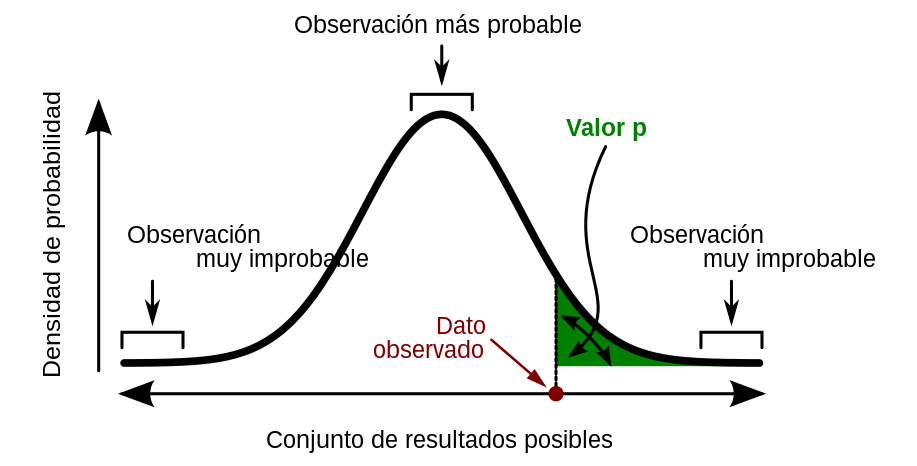
\includegraphics[width=0.7\linewidth]{material/img/Valor_p} 

}

\caption{Estadístico de prueba para un prueba altenativa con signo $>$}\label{fig:graficovalorp}
\end{figure}

La tabla \ref{tab:regiones}, da cuenta de la relación que existe entre las pruebas de hipótesis y la ubicación del valor-p en el gráfico presentado.

\begin{table}[H]
\centering
\caption{\label{tab:regiones}Hipótesis alternativa, valor-p y estadístico de prueba}
\centering
\resizebox{\ifdim\width>\linewidth\linewidth\else\width\fi}{!}{
\begin{tabular}[t]{>{\centering\arraybackslash}p{4cm}>{\centering\arraybackslash}p{4cm}>{\centering\arraybackslash}p{5cm}}
\toprule
Signo de comparación en $H_1$ & Referencia & Ubicación del estadístico de prueba y valor-p\\
\midrule
$>$ & Unilateral derecha & A la derecha del gráfico\\
$<$ & Unilateral izquierda & A la izquierda del gráfico\\
$\neq$ & Bilateral & A ambos lados del gráfico\\
\bottomrule
\end{tabular}}
\end{table}

La regla de rechazo usando el valor-p es

\[\text{Rechazar } H_0 \text{ si el valor-p } \leq \alpha\]

En la figura \ref{fig:regiones3}, se puede observar los tres casos posibles para las distintas hipótesis alternativas, en las cuales se ejemplifica un valor-p en cada uno de los casos. De izquierda a derecha, las hipótesis alternativas correspondientes son unilateral izquierda, unilateral derecha, y bilateral.

\begin{figure}

{\centering 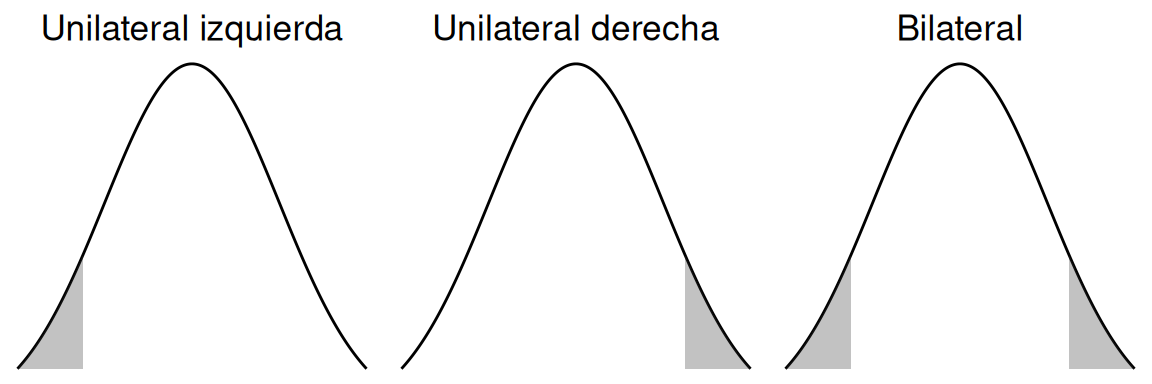
\includegraphics[width=\linewidth]{est2+inferencia_files/figure-latex/regiones3-1} 

}

\caption{Valores -p por tipo de hipótesis alternativa}\label{fig:regiones3}
\end{figure}

La decisión de si en cada uno de los casos se rechaza o no la hipótesis nula, depende del valor elegido para la significancia. En la figura \ref{fig:areas-rechazo-ud} se muestra la comparativa entre el valor-p y \(\alpha\) para el caso de una hipótesis alternativa unilateral derecha; el área sombreada de color rojo corresponde al valor de \(\alpha\) (\textbf{área de rechazo}), mientras que el área sombreada de color gris corresponde al valor-p definido por el estadístico de prueba.

\begin{figure}

{\centering 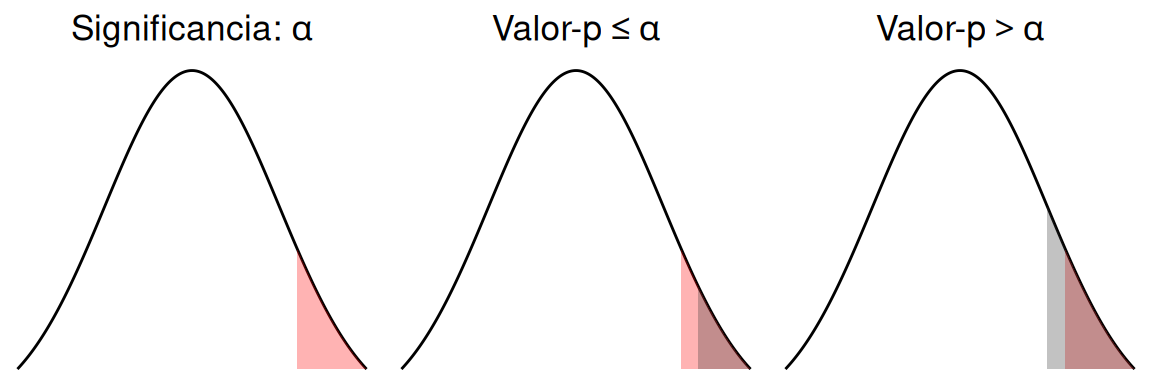
\includegraphics[width=\linewidth]{est2+inferencia_files/figure-latex/areas-rechazo-ud-1} 

}

\caption{Comparativa del valor-p y el área de rechazo para una prueba unilateral derecha}\label{fig:areas-rechazo-ud}
\end{figure}

Cabe recordar que, el valor de alfa (valor del área roja en la figura \ref{fig:areas-rechazo-ud}) estará dado por el investigador (subjetivo), mientras que el valor del área gris se debe determinar a partir de los datos de la muestra (estadístico de prueba).

\begin{enumerate}
\def\labelenumi{\arabic{enumi}.}
\setcounter{enumi}{1}
\tightlist
\item
  \textbf{Método del valor crítico}
\end{enumerate}

Este método consiste en comparar el estadístico de prueba con un número fijo llamado \textbf{valor crítico}. El valor crítico es un punto de referencia para determinar si el valor del estadístico de prueba es lo suficientemente pequeño para rechazar la hipótesis nula. El valor
crítico corresponde a la coordenada del eje horizontal que define el área llamada \(\alpha\) (fijado por el investigador), y está ubicada en el mismo sector que el valor-p.~

El intervalo de números generado a partir del valor crítico es lo denominado \textbf{región de rechazo}. En la figura \ref{fig:region-rechazo-1}, se observa que una hipótesis nula es rechazada cuando el valor-p es menor o igual a \(\alpha\), lo cual, es equivalente a decir que (gráfico de la izquierda), el estadístico de prueba (1.4) es mayor o igual al valor crítico (0.8), a esto se le denomina ``caer en la región de rechazo''. El razonamiento de rechazo utilizando el valor crítico depende de la zona en la que se ubica alfa y el valor-p.

\begin{figure}

{\centering 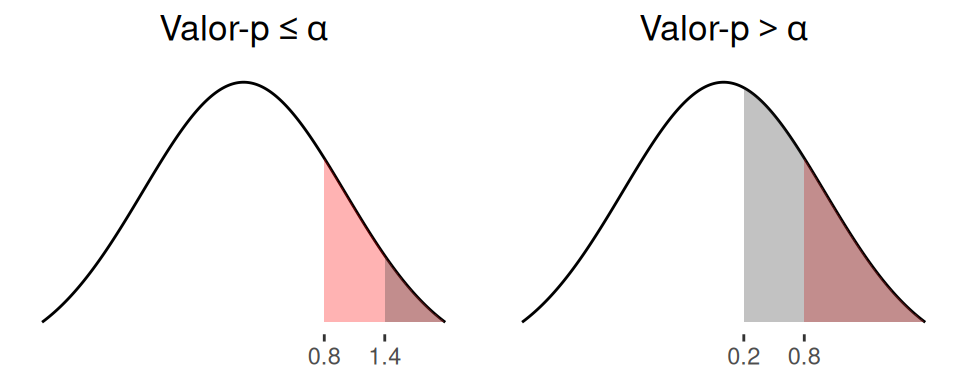
\includegraphics{est2+inferencia_files/figure-latex/region-rechazo-1-1} 

}

\caption{Método del valor crítico para una hipótesis unilateral derecha}\label{fig:region-rechazo-1}
\end{figure}

Los lineamientos de cómo construir un estadístico de prueba, determinar el varlo crítico y el valor-p asociados a una prueba de hipótesis, se darán a conocer a partir de la sección \ref{pruebas}.

\subsection{Intervalos de confianza}\label{prueba-de-hipotesis-intervalos-de-confianza}

Existe un relación directa entre las pruebas de hipótesis y los intervalos de confianza, ya que estos pueden ser utilizados para rechazar o no \(H_0\). La tabla \ref{tab:ICpruebas}, da cuenta de del tipo de intervalo de confianza que se debe elaborar para cada tipo de prueba de hipótesis.

\begin{table}[H]
\centering
\caption{\label{tab:ICpruebas}Hipótesis alternativa e Intervalo de confianza}
\centering
\begin{tabular}[t]{cc}
\toprule
Signo de comparación en $H_1$ & Tipo de intervalo de confianza\\
\midrule
$>$ & $(a,\infty )$\\
$<$ & $(-\infty ,b)$\\
$\neq$ & $(a,b)$\\
\bottomrule
\end{tabular}
\end{table}

A lo largo de las distintas pruebas, se abordarán los distintos métodos de prueba, incluyendo el uso de intervalos de confianza.

\section{Prueba de hipótesis para una media}\label{pruebas}

Esta sección se centra en el planteamiento y prueba de hipótesis relacionadas a la parámetro de media. Para cada uno de estos casos, se detalla el procedimiento en R y los distintos métodos de prueba para la decisión de rechazo de \(H_0\). En particular, las pruebas para este parámetro requieren que la distribución poblacional de la variable de estudio es normal, lo cual, se asumirá en los enunciados de los ejercicios y/o ejemplos según corresponda.

\subsection{Varianza poblacional conocida}\label{prueba-de-hipotesis-media-varianza-conocida}

Aun cuando la suposición de que el valor de \(\sigma^2\) es conocido, rara vez se cumple en la práctica. Este caso proporciona un buen punto de partida debido a la facilidad con que los procedimientos generales y sus propiedades pueden ser desarrollados. La hipótesis nula en los tres casos propondrá que \(\mu\) tiene un valor numérico particular, el valor nulo, el cual será denotado por \(\mu_0\).

El estadístico de prueba y los valores críticos de comparación están dados en la tabla \ref{tab:unamedia1}.

\begin{table}[H]
\centering
\caption{\label{tab:unamedia1}Método del valor crítico para la prueba de una media con varianza poblacional conocida}
\centering
\resizebox{\ifdim\width>\linewidth\linewidth\else\width\fi}{!}{
\begin{tabular}[t]{llll}
\toprule
Hipótesis nula & Estadístico de prueba & Hipótesis alternativa & Criterio de rechazo\\
\midrule
 &  & $H_1: \mu \neq \mu_0$ & $|Z_0| \geq Z_{1-\alpha/2}$\\
\cmidrule{3-4}
 &  & $H_1: \mu \gt \mu_0$ & $Z_0 \geq Z_{1-\alpha}$\\
\cmidrule{3-4}
\multirow{-3}{*}{\raggedright\arraybackslash $H_0: \mu = \mu_0$} & \multirow{-3}{*}{\raggedright\arraybackslash $Z_0 = \displaystyle\frac{\bar{x}-\mu_0}{\sigma/\sqrt{n}}$} & $H_1: \mu \lt \mu_0$ & $Z_0 \leq Z_{\alpha}$\\
\bottomrule
\end{tabular}}
\end{table}

\begin{example}

El índice Rockwell de dureza para acero se determina al presionar una punta de diamante en el acero y medir la profundidad de la penetración, el cual tiene un varianza de medición de 6. Para 50 especímenes de una aleación de acero, el índice Rockwell de dureza promedió 62. El fabricante dice que esta aleación tiene un índice de dureza promedio menor a 64. Asumiendo que el índice de dureza sigue una distribución normal, ¿hay suficiente evidencia para refutar lo dicho por el fabricante con un nivel de significancia de 1\%?

Al plantear la prueba de hipótesis se debe tener en cuenta que la hipótesis del investigador ha de estar reflejada en \(H_1\), tal como se muestra a continuación.

\begin{itemize}
\tightlist
\item
  \(\mu\): media del índice de dureza de la aleación de acero.
\end{itemize}

\begin{equation}
\notag
\begin{split}
H_0&: \mu = 64\\
H_1&: \mu < 64
\end{split}
\end{equation}

\begin{enumerate}
\def\labelenumi{\arabic{enumi}.}
\item
  \textbf{Método del valor-p}

  Verificación del criterio de rechazo: Valor-p \(\leq \alpha\).

\begin{Shaded}
\begin{Highlighting}[]
\CommentTok{\# Cálculo del estadístico de prueba}
\NormalTok{z0 }\OtherTok{=}\NormalTok{ (}\DecValTok{62{-}64}\NormalTok{)}\SpecialCharTok{/}\NormalTok{(}\FunctionTok{sqrt}\NormalTok{(}\DecValTok{6}\NormalTok{)}\SpecialCharTok{/}\FunctionTok{sqrt}\NormalTok{(}\DecValTok{50}\NormalTok{))}
\NormalTok{z0}
\end{Highlighting}
\end{Shaded}

\begin{verbatim}
## [1] -5.773503
\end{verbatim}

\begin{Shaded}
\begin{Highlighting}[]
\CommentTok{\# Cálculo del valor{-}p}
\NormalTok{valor\_p }\OtherTok{=} \FunctionTok{pnorm}\NormalTok{(z0)}
\NormalTok{valor\_p}
\end{Highlighting}
\end{Shaded}

\begin{verbatim}
## [1] 3.882018e-09
\end{verbatim}

\begin{Shaded}
\begin{Highlighting}[]
\CommentTok{\# Verificación el criterio}
\NormalTok{valor\_p }\SpecialCharTok{\textless{}=} \FloatTok{0.01}
\end{Highlighting}
\end{Shaded}

\begin{verbatim}
## [1] TRUE
\end{verbatim}

  \textbf{Interpretación utilizando el método del valor-p}: El valor-p de 3.88 \(\times 10^{-9}\) es menor o igual a la significancia del 0.01, por lo cual, existe suficiente evidencia estadística para rechazar la hipótesis nula, es decir, existe suficiente evidencia para apoyar la afirmación de que la media del índice de dureza de la aleación de acero es menor a 64. Considerando una confianza del 99\%.
\item
  \textbf{Método del valor crítico}

  En caso de que deseemos utilizar el método del valor-p, es necesario apoyarnos en R para realizar el calculo de este. El comando necesario para calcular el valor depende la prueba que estemos llevando a cabo, por lo que en el siguiente \href{material/resumenes/Rechazo.pdf}{documento} podrán encontrar un resumen para las distintas pruebas.

  Verificación del criterio de rechazo: \(Z_0 \leq Z_{\alpha}\).

\begin{Shaded}
\begin{Highlighting}[]
\CommentTok{\# Cálculo del valor crítico}
\NormalTok{valor\_critico }\OtherTok{=} \FunctionTok{qnorm}\NormalTok{(}\FloatTok{0.01}\NormalTok{)}
\NormalTok{valor\_critico}
\end{Highlighting}
\end{Shaded}

\begin{verbatim}
## [1] -2.326348
\end{verbatim}

\begin{Shaded}
\begin{Highlighting}[]
\CommentTok{\# Verificación del criterio}
\NormalTok{z0 }\SpecialCharTok{\textless{}=}\NormalTok{ valor\_critico}
\end{Highlighting}
\end{Shaded}

\begin{verbatim}
## [1] TRUE
\end{verbatim}

  \textbf{Interpretación utilizando el método del valor crítico}: El valor del estadístico de prueba de -5.7735 es menor o igual al valor crítico de -2.3263, por lo cual, existe suficiente evidencia estadística para rechazar la hipótesis nula, es decir, existe suficiente evidencia para apoyar la afirmación de que la media del índice de dureza de la aleación de acero es menor a 64. Considerando una confianza del 99\%.
\item
  \textbf{Método del intervalo de confianza}

  Al igual que el valor-p, la forma en la que se debe usar el intervalo de confianza varía dependiendo del tipo de prueba de hipótesis que se realiza, por lo que en el siguiente \href{material/resumenes/hipotesis+ic.pdf}{documento} podrán encontrar un resumen para las distintas pruebas, dicho documento incluye los distintos comando en R para obtener los resultados de una prueba de hipótesis de manera automática.

  Verificación del criterio de rechazo: \(\mu_0 \notin\) IC.

  El intervalo de confianza a construir es:

  \begin{equation}
    \notag
    \left(-\infty, \bar{x} + Z_{1-\alpha}\frac{\sigma}{\sqrt{n}}\right)
  \end{equation}

\begin{Shaded}
\begin{Highlighting}[]
\CommentTok{\# Cálculo de los límites del intervalo de confianza}
\NormalTok{Limite\_superior }\OtherTok{=} \DecValTok{62} \SpecialCharTok{+} \FunctionTok{qnorm}\NormalTok{(}\FloatTok{0.99}\NormalTok{)}\SpecialCharTok{*}\FunctionTok{sqrt}\NormalTok{(}\DecValTok{6}\NormalTok{)}\SpecialCharTok{/}\FunctionTok{sqrt}\NormalTok{(}\DecValTok{50}\NormalTok{)}
\NormalTok{Limite\_superior}
\end{Highlighting}
\end{Shaded}

\begin{verbatim}
## [1] 62.80587
\end{verbatim}

\begin{Shaded}
\begin{Highlighting}[]
\CommentTok{\# Verificación del criterio}
\DecValTok{64} \SpecialCharTok{\textgreater{}}\NormalTok{ Limite\_superior}
\end{Highlighting}
\end{Shaded}

\begin{verbatim}
## [1] TRUE
\end{verbatim}

  \textbf{Interpretación utilizando el método del intervalo de confianza}: El intervalo de confianza \((-\infty, 62.8058)\) no contiene al valor de \(\mu_0 = 64\), por lo cual, existe suficiente evidencia estadística para rechazar la hipótesis nula, es decir, existe suficiente evidencia para apoyar la afirmación de que la media del índice de dureza de la aleación de acero es menor a 64. Considerando una confianza del 99\%.
\end{enumerate}

\end{example}

Para este tipo de pruebas, no hay comandos en R que permitan hacer el trabajo de manera automática. Esto es debido a lo expuesto en un principio: \textbf{difícilmente se conoce la varianza poblacional en la práctica}.

\begin{exercise}

Sea el estadístico de prueba \(Z_0\) con una distribución normal estándar cuando \(H_0\) es verdadera. Dé el nivel de significación en cada una de las siguientes situaciones:

\begin{enumerate}
\def\labelenumi{\alph{enumi}.}
\tightlist
\item
  \(H_1: \mu > \mu_0\), región de rechazo \(Z_0\geq 1.88\).
\item
  \(H_1: \mu < \mu_0\), región de rechazo \(Z_0\leq -2.75\).
\item
  \(H_1: \mu \neq \mu_0\), región de rechazo \(Z_0\geq 2.88\) o \(Z_0\leq -2.88\).
\end{enumerate}

\end{exercise}

\begin{exercise}
Un fabricante de cajas de cartón afirma que sus cajas tienen un peso promedio de 5 kg. Para verificar esta afirmación, un cliente selecciona al azar 25 cajas y encuentra que el peso promedio es de 4.8 kg con una desviación estándar conocida de 0.5 kg. ¿Hay suficiente evidencia para rechazar la afirmación del fabricante al nivel de significancia del 5\%?
\end{exercise}

\begin{exercise}
Se sabe que la duración de las baterías sigue una distribución normal con media 290 horas y varianza poblacional conocida de 64 horas. Bajo una nueva fórmula de fabricación, se tomó una muestra aleatoria de 36 dispositivos móviles y se registró una duración media muestral de 280 horas. Utilizando un nivel de significancia del 5\%, ¿se puede concluir con suficiente evidencia estadística que la duración media de las baterías ha mejorado significativamente después de aplicar una nueva fórmula en su fabricación?
\end{exercise}

\begin{exercise}
Un cirujano necesita evaluar si los pacientes se recuperan en un promedio en un tiempo menor a 5 días después de una cirugía. Para probar su afirmación, un internista toma una muestra aleatoria de 20 pacientes y encuentra que la duración promedio de recuperación es de 6 días, con una desviación estándar conocida de 1.5 días. ¿Hay suficiente evidencia para rechazar la afirmación del cirujano al nivel de significancia del 10\%?
\end{exercise}

\begin{exercise}
Se requiere estudiar si la cantidad promedio de cafeína en una taza de café es menor a 100 mg. Para probar esta hipótesis, se toma una muestra aleatoria de 50 tazas de café y se encuentra que la cantidad promedio de cafeína es de 105 mg, con una desviación estándar conocida de 15 mg. ¿Hay suficiente evidencia para rechazar la hipótesis nula al nivel de significancia del 5\%?
\end{exercise}

\begin{exercise}
Se desea evaluar si la altura promedio de una población de girasoles es distinta de 150 cm. Para ello, se selecciona una muestra aleatoria de 30 girasoles y se encuentra que la altura promedio es de 155 cm, con una desviación estándar conocida de 5 cm. ¿Hay suficiente evidencia para rechazar la hipótesis nula al nivel de significancia del 1\%?
\end{exercise}

\subsection{Varianza poblacional desconocida}\label{prueba-de-hipotesis-media-varianza-desconocida}

De igual manera a lo expuesto en el primer caso, los pasos a seguir para probar una hipótesis son los mismos, y se mantendrá así para cualquier caso.

\begin{enumerate}
\def\labelenumi{\arabic{enumi}.}
\tightlist
\item
  Plantear las hipótesis nula y alternativa
\item
  Identificar o establecer el nivel de significancia.
\item
  Identificar los datos muestrales y poblacionales con los que se cuenta.
\item
  Utilizar alguna de las reglas de decisión (Estadístico de prueba, valor-p o intervalo de confianza).
\item
  Concluir
\end{enumerate}

En la situación de una prueba de hipótesis de la media, en la cual lo datos distribuyen normal y la varianza poblacional es desconocida, los criterios de rechazo son similares a los vistos anteriormente, sin embargo, cambia la distribución del estadístico de prueba, tal como se muestra en la tabla \ref{tab:unamedia2}.

\begin{table}[H]
\centering
\caption{\label{tab:unamedia2}Método del valor crítico para la prueba de una media con varianza poblacional desconocida}
\centering
\resizebox{\ifdim\width>\linewidth\linewidth\else\width\fi}{!}{
\begin{tabular}[t]{llll}
\toprule
Hipótesis nula & Estadístico de prueba & Hipótesis alternativa & Criterio de rechazo\\
\midrule
 &  & $H_1: \mu \neq \mu_0$ & $|t_0| \geq t_{1-\alpha/2, n-1}$\\
\cmidrule{3-4}
 &  & $H_1: \mu \gt \mu_0$ & $t_0 \geq t_{1-\alpha,n-1}$\\
\cmidrule{3-4}
\multirow{-3}{*}{\raggedright\arraybackslash $H_0: \mu = \mu_0$} & \multirow{-3}{*}{\raggedright\arraybackslash $t_0 = \displaystyle\frac{\bar{x}-\mu_0}{S/\sqrt{n}}$} & $H_1: \mu \lt \mu_0$ & $t_0 \leq t_{\alpha,n-1}$\\
\bottomrule
\end{tabular}}
\end{table}

donde \(n\) corresponde al tamaño de la muestra.

\begin{example}
\protect\hypertarget{exm:imacec}{}\label{exm:imacec}

Utilizando la base de datos \hyperref[Imacec2]{Imacec}, establezca si hay suficiente evidencia estadística para afirmar que, el valor promedio del Imacec de cada sector por separado es mayor a 98.54167 (denote este valor por \(\mu_0\)). Establezca las hipótesis respectivas, estadísticos y criterios de rechazo, utilizando una significancia del 10\%. Asuma que las variables distribuyen normal y tienen varianza poblacional desconocida.

En este caso al contar con una base de datos (y para este tipo de prueba), podemos hacer uso directamente de R para obtener el estadístico de prueba, valor-p e intervalo de confianza asociado.

Iniciamos con la prueba de hipótesis para el sector de minería.

\begin{itemize}
\tightlist
\item
  \(\mu:\) Media del Imacec de Minería.
\end{itemize}

\begin{equation}
    \notag
    \begin{split}
        H_0: \mu = 98.54167\\
        H_1: \mu > 98.54167
    \end{split}
\end{equation}

Luego, haciendo uso de R obtenemos los elementos necesario para rechazar o no \(H_0\).

\begin{Shaded}
\begin{Highlighting}[]
\CommentTok{\# Cargue previamente la base de datos, guardándola con el nombre "df"}
\CommentTok{\# Minería}
\FunctionTok{t.test}\NormalTok{( }\CommentTok{\# Prueba de hipótesis para el estadístico con distribución t{-}student}
  \AttributeTok{x =}\NormalTok{ df}\SpecialCharTok{$}\NormalTok{Mineria, }\CommentTok{\# Valores del Imacec de Minería}
  \AttributeTok{alternative =} \StringTok{"greater"}\NormalTok{, }\CommentTok{\# Signo de desigualdad de la hipótesis alternativa}
  \AttributeTok{mu =} \FloatTok{98.54167}\NormalTok{, }\CommentTok{\# Valor del Mu\_0}
  \AttributeTok{conf.level =} \FloatTok{0.9} \CommentTok{\# Confianza = 1 {-} alfa}
\NormalTok{  )}
\end{Highlighting}
\end{Shaded}

\begin{verbatim}
## 
##  One Sample t-test
## 
## data:  df$Mineria
## t = -1.2773, df = 53, p-value = 0.8965
## alternative hypothesis: true mean is greater than 98.54167
## 90 percent confidence interval:
##  96.21024      Inf
## sample estimates:
## mean of x 
##  97.38519
\end{verbatim}

\begin{enumerate}
\def\labelenumi{\arabic{enumi}.}
\item
  \textbf{Método del valor-p}

  Verificación del criterio de rechazo: Valor-p \(\leq \alpha\).

\begin{Shaded}
\begin{Highlighting}[]
\CommentTok{\# Cálculo del valor{-}p}
\NormalTok{valor\_p }\OtherTok{=} \FloatTok{0.8965}
\CommentTok{\# Verificación el criterio}
\NormalTok{valor\_p }\SpecialCharTok{\textless{}=} \FloatTok{0.1}
\end{Highlighting}
\end{Shaded}

\begin{verbatim}
## [1] FALSE
\end{verbatim}

  \textbf{Interpretación utilizando el método del valor-p}: El valor-p de 0.8965 no es menor o igual a la significancia del 0.1, por lo cual, no existe suficiente evidencia estadística para rechazar la hipótesis nula, es decir, no existe suficiente evidencia para apoyar la afirmación de que el valor promedio del Imacec del sector de Minería es mayor a 98.54167. Considerando una confianza del 90\%.
\item
  \textbf{Método del valor crítico}

  Verificación del criterio de rechazo: \(t_0 \geq t_{1-\alpha,n-1}\).

\begin{Shaded}
\begin{Highlighting}[]
\CommentTok{\# Cálculo del valor crítico}
\NormalTok{valor\_critico }\OtherTok{=} \FunctionTok{qt}\NormalTok{(}\DecValTok{1}\FloatTok{{-}0.1}\NormalTok{, }\AttributeTok{df =} \DecValTok{53}\NormalTok{)}
\NormalTok{valor\_critico}
\end{Highlighting}
\end{Shaded}

\begin{verbatim}
## [1] 1.29773
\end{verbatim}

\begin{Shaded}
\begin{Highlighting}[]
\CommentTok{\# Verificación el criterio}
\NormalTok{t0 }\OtherTok{=} \SpecialCharTok{{-}}\FloatTok{1.2773}
\NormalTok{t0 }\SpecialCharTok{\textgreater{}=}\NormalTok{ valor\_critico}
\end{Highlighting}
\end{Shaded}

\begin{verbatim}
## [1] FALSE
\end{verbatim}

  \textbf{Interpretación utilizando el método del valor crítico}: El estadístico de prueba de -1.2773 no es mayor o igual al valor crítico de 1.2977, por lo cual, no existe suficiente evidencia estadística para rechazar la hipótesis nula, es decir, no existe suficiente evidencia para apoyar la afirmación de que el valor promedio del Imacec del sector de Minería es mayor a 98.54167. Considerando una confianza del 90\%.
\item
  \textbf{Método del intervalo de confianza}

  Verificación del criterio de rechazo: \(\mu_0 \notin\) IC.

\begin{Shaded}
\begin{Highlighting}[]
\CommentTok{\# Verificación del criterio}
\NormalTok{Limite\_inferior }\OtherTok{=} \FloatTok{96.21024}
\FloatTok{98.54167} \SpecialCharTok{\textless{}}\NormalTok{ Limite\_inferior}
\end{Highlighting}
\end{Shaded}

\begin{verbatim}
## [1] FALSE
\end{verbatim}

  \textbf{Interpretación utilizando el método del intervalo de confianza}: El intervalo de confianza \((96.21024, \infty)\) contiene al valor de \(\mu_0 = 98.54167\), por lo cual, no existe suficiente evidencia estadística para rechazar la hipótesis nula, es decir, no existe suficiente evidencia para apoyar la afirmación de que el valor promedio del Imacec del sector de Minería es mayor a 98.54167. Considerando una confianza del 90\%.
\end{enumerate}

La prueba de hipótesis para el sector de industria es la siguiente.

\begin{itemize}
\tightlist
\item
  \(\mu:\) Media del Imacec de Industria.
\end{itemize}

\begin{equation}
    \notag
    \begin{split}
        H_0: \mu = 98.54167\\
        H_1: \mu > 98.54167
    \end{split}
\end{equation}

\begin{Shaded}
\begin{Highlighting}[]
\CommentTok{\# Industria}
\FunctionTok{t.test}\NormalTok{( }\CommentTok{\# Prueba de hipótesis para el estadístico con distribución t{-}student}
  \AttributeTok{x =}\NormalTok{ df}\SpecialCharTok{$}\NormalTok{Industria, }\CommentTok{\# Valores del Imacec de Industria}
  \AttributeTok{alternative =} \StringTok{"greater"}\NormalTok{, }\CommentTok{\# Signo de desigualdad de la hipótesis alternativa}
  \AttributeTok{mu =} \FloatTok{98.54167}\NormalTok{, }\CommentTok{\# Valor del Mu\_0}
  \AttributeTok{conf.level =} \FloatTok{0.9} \CommentTok{\# Confianza = 1 {-} alfa}
\NormalTok{  )}
\end{Highlighting}
\end{Shaded}

\begin{verbatim}
## 
##  One Sample t-test
## 
## data:  df$Industria
## t = 1.3678, df = 53, p-value = 0.08857
## alternative hypothesis: true mean is greater than 98.54167
## 90 percent confidence interval:
##  98.60095      Inf
## sample estimates:
## mean of x 
##  99.69815
\end{verbatim}

\begin{enumerate}
\def\labelenumi{\arabic{enumi}.}
\item
  \textbf{Método del valor-p}

  Verificación del criterio de rechazo: Valor-p \(\leq \alpha\).

\begin{Shaded}
\begin{Highlighting}[]
\CommentTok{\# Cálculo del valor{-}p}
\NormalTok{valor\_p }\OtherTok{=} \FloatTok{0.08857}
\CommentTok{\# Verificación el criterio}
\NormalTok{valor\_p }\SpecialCharTok{\textless{}=} \FloatTok{0.1}
\end{Highlighting}
\end{Shaded}

\begin{verbatim}
## [1] TRUE
\end{verbatim}

  \textbf{Interpretación utilizando el método del valor-p}: El valor-p de 0.8965 menor o igual a la significancia del 0.1, por lo cual, existe suficiente evidencia estadística para rechazar la hipótesis nula, es decir, existe suficiente evidencia para apoyar la afirmación de que el valor promedio del Imacec del sector de Industria es mayor a 98.54167. Considerando una confianza del 90\%.
\item
  \textbf{Método del valor crítico}

  Verificación del criterio de rechazo: \(t_0 \geq t_{1-\alpha,n-1}\).

\begin{Shaded}
\begin{Highlighting}[]
\CommentTok{\# Cálculo del valor crítico}
\NormalTok{valor\_critico }\OtherTok{=} \FunctionTok{qt}\NormalTok{(}\DecValTok{1}\FloatTok{{-}0.1}\NormalTok{, }\AttributeTok{df =} \DecValTok{53}\NormalTok{)}
\NormalTok{valor\_critico}
\end{Highlighting}
\end{Shaded}

\begin{verbatim}
## [1] 1.29773
\end{verbatim}

\begin{Shaded}
\begin{Highlighting}[]
\CommentTok{\# Verificación el criterio}
\NormalTok{t0 }\OtherTok{=} \FloatTok{1.3678}
\NormalTok{t0 }\SpecialCharTok{\textgreater{}=}\NormalTok{ valor\_critico}
\end{Highlighting}
\end{Shaded}

\begin{verbatim}
## [1] TRUE
\end{verbatim}

  \textbf{Interpretación utilizando el método del valor crítico}: El estadístico de prueba de 1.3678 es mayor o igual al valor crítico de 1.2977, por lo cual, existe suficiente evidencia estadística para rechazar la hipótesis nula, es decir, existe suficiente evidencia para apoyar la afirmación de que el valor promedio del Imacec del sector de Industria es mayor a 98.54167. Considerando una confianza del 90\%.
\item
  \textbf{Método del intervalo de confianza}

  Verificación del criterio de rechazo: \(\mu_0 \notin\) IC.

\begin{Shaded}
\begin{Highlighting}[]
\CommentTok{\# Verificación del criterio}
\NormalTok{Limite\_inferior }\OtherTok{=} \FloatTok{98.6009}
\FloatTok{98.54167} \SpecialCharTok{\textless{}}\NormalTok{ Limite\_inferior}
\end{Highlighting}
\end{Shaded}

\begin{verbatim}
## [1] TRUE
\end{verbatim}

  \textbf{Interpretación utilizando el método del intervalo de confianza}: El intervalo de confianza \((98.6009, \infty)\) no contiene al valor de \(\mu_0 = 98.54167\), por lo cual, existe suficiente evidencia estadística para rechazar la hipótesis nula, es decir, existe suficiente evidencia para apoyar la afirmación de que el valor promedio del Imacec del sector de Industria es mayor a 98.54167. Considerando una confianza del 90\%.
\end{enumerate}

\end{example}

\begin{exercise}
Utilizando la base de datos \hyperref[Imacec2]{Imacec}, establezca si hay suficiente evidencia estadística para afirmar que, el valor promedio del Imacec de cada sector durante el año 2022 es mayor 96.89167. Establezca las hipótesis, estadísticos y criterios de rechazo. Utilice una significancia del 7\%. Además, asuma que las variables distribuyen normal y tienen varianza poblacional desconocida. Concluya.
\end{exercise}

\begin{exercise}
\protect\hypertarget{exr:metano}{}\label{exr:metano}El control de emisión de residuos ha sido un tema que ha cobrado gran importancia en los últimos 20 años debido a los efectos del calentamiento global. Uno de los tantos residuos que contamina el aire es el Metano (CH4). Para estudiar este fenómeno haremos uso de la base \href{https://raw.githubusercontent.com/Dfranzani/Bases-de-datos-para-cursos/main/2022-2/Estad\%C3\%ADstica\%202/metano.csv}{\emph{metano.csv}}, la cual contiene los siguientes datos:

\begin{itemize}
\tightlist
\item
  Año: año en el que se realiza la medición de emisión de CH4.
\item
  Mes: mes del año en el que se realiza la medición de emisión de CH4.
\item
  CH4: concentración de CH4 (partes por miles de millones) en un muestra de aire.
\end{itemize}

Establezca si hay suficiente evidencia estadística para afirmar lo siguiente:

\begin{enumerate}
\def\labelenumi{\arabic{enumi}.}
\tightlist
\item
  La concentración promedio de metano es distinta a 1700 partes por miles de millones.
\item
  La concentración promedio de metano del año 2021 es superior a 1780 partes por miles de millones.
\item
  La concentración promedio de metano del periodo en el periodo de años 2019 - 2022 (inclusive) es inferior a 1750 partes por miles de millones.
\end{enumerate}

Establezca las hipótesis respectivas, estadísticos y criterios de rechazo, utilice una significancia del 7\%. Asuma que las variables distribuyen normal y tienen varianza poblacional desconocida. Concluya.
\end{exercise}

\begin{exercise}
\protect\hypertarget{exr:consumidor}{}\label{exr:consumidor}Utilizando la base de datos \hyperref[ICC]{ICC}, estudie si hay suficiente evidencia estadística para afirmar lo siguiente:

\begin{enumerate}
\def\labelenumi{\arabic{enumi}.}
\tightlist
\item
  El promedio del ICC es distinto a 100 puntos.
\item
  El promedio del ICC en Francia es menor a 105 puntos.
\item
  El promedio del ICC en Alemania es mayor a 107 puntos.
\end{enumerate}

Establezca las hipótesis, estadísticos y criterios de rechazo. Utilice una significancia del 12\%. Además, asuma que las variables distribuyen normal y tienen varianza poblacional desconocida. Concluya.
\end{exercise}

\section{Prueba de hipótesis para la diferencia de medias}\label{prueba-de-hipotesis-diferencia-de-medias}

En esta sección se continúa con el estudio de la inferencia estadística, específicamente para la diferencia entre dos medias poblacionales. Por ejemplo, quizá desee obtener una estimación por intervalo para la diferencia entre el salario inicial medio de la población de hombres y el salario inicial medio de la población de mujeres \citep[página 395]{anderson}. Para este tipo de pruebas, se requiere que las distribuciones poblacionales de las variables sean normales e independientes, lo cual, se asumirá en los enunciados de ejemplos y/o ejercicios según corresponda.

\subsection{Varianzas poblacionales conocidas}\label{prueba-de-hipotesis-diferencia-de-medias-varianzas-conocidas}

El primero de los tres casos corresponde al de varianzas poblacionales conocidas. La tabla \ref{tab:dosmedias1} da cuenta del estadístico de prueba asociado las respectivas hipótesis, además de los criterios asociados al valor crítico correspondiente.

\begin{table}[H]
\centering
\caption{\label{tab:dosmedias1}Método del valor crítico para la prueba de diferencia de medias con varianzas poblacionales conocidas}
\centering
\resizebox{\ifdim\width>\linewidth\linewidth\else\width\fi}{!}{
\begin{tabular}[t]{llll}
\toprule
Hipótesis nula & Estadístico de prueba & Hipótesis alternativa & Criterio de rechazo\\
\midrule
 &  & $H_1: \mu_X - \mu_Y \neq \delta_0$ & $|Z_0| \geq Z_{1-\alpha/2}$\\
\cmidrule{3-4}
 &  & $H_1: \mu_X - \mu_Y \gt \delta_0$ & $Z_0 \geq Z_{1-\alpha}$\\
\cmidrule{3-4}
\multirow{-3}{*}{\raggedright\arraybackslash $H_0: \mu_X - \mu_Y = \delta_0$} & \multirow{-3}{*}{\raggedright\arraybackslash $Z_0 = \displaystyle\frac{\bar{x} - \bar{y} - \delta_0}{\sqrt{\sigma^2_X/n_X + \sigma^2_Y/n_Y}}$} & $H_1: \mu_X - \mu_Y \lt \delta_0$ & $Z_0 \leq Z_{\alpha}$\\
\bottomrule
\end{tabular}}
\end{table}

\begin{example}

En dos ciudades se llevó acabo una encuesta sobre el costo de la vida, en relación al gasto promedio en alimentación en familias constituidas por cuatro personas. De cada ciudad se seleccionó aleatoriamente una muestra de 20 familias y se observaron sus gastos semanales en alimentación. Las medias muestrales y desviaciones estándar poblacionales fueron las siguientes:

\begin{equation}
\notag
\begin{split}
\bar{x} = 135, & \text{ } \sigma_X = 15\\
\bar{y} = 122, & \text{ } \sigma_Y = 10
\end{split}
\end{equation}

Si se supone que se muestrearon dos poblaciones independientes con distribución normal cada una, analizar si existe una diferencia real entre ambas medias. Considere una confianza del 95\%.

Las hipótesis a plantear son las siguientes.

\begin{itemize}
\tightlist
\item
  \(\mu_X:\) gasto medio semanal en alimentación en la ciudad X.
\item
  \(\mu_Y:\) gasto medio semanal en alimentación en la ciudad Y.
\end{itemize}

\begin{equation}
\notag
  \begin{split}
    H_0&: \mu_{X} - \mu_{Y} = 0\\
    H_1&: \mu_{X} - \mu_{Y} \neq 0\\
  \end{split}
\end{equation}

Al igual que en la prueba para una media cuando se conoce la varianza poblacional, esta prueba no tiene una implementación directa en R, por lo que construiremos manualmente los métodos de rechazo.

\begin{Shaded}
\begin{Highlighting}[]
\NormalTok{x.barra }\OtherTok{=} \DecValTok{135}
\NormalTok{y.barra }\OtherTok{=} \DecValTok{122}
\NormalTok{sigma.x }\OtherTok{=} \DecValTok{15}
\NormalTok{sigma.y }\OtherTok{=} \DecValTok{10}
\NormalTok{nx }\OtherTok{=} \DecValTok{20}
\NormalTok{ny }\OtherTok{=} \DecValTok{20}
\NormalTok{alfa }\OtherTok{=} \FloatTok{0.05}
\NormalTok{delta0 }\OtherTok{=} \DecValTok{0}
\end{Highlighting}
\end{Shaded}

\begin{enumerate}
\def\labelenumi{\arabic{enumi}.}
\item
  \textbf{Método del valor-p}

  Verificación del criterio de rechazo: Valor-p \(\leq \alpha\).

\begin{Shaded}
\begin{Highlighting}[]
\CommentTok{\# Cálculo del estadístico de prueba}
\NormalTok{z0 }\OtherTok{=}\NormalTok{ (x.barra }\SpecialCharTok{{-}}\NormalTok{ y.barra }\SpecialCharTok{{-}}\NormalTok{ delta0)}\SpecialCharTok{/}\FunctionTok{sqrt}\NormalTok{(sigma.x}\SpecialCharTok{\^{}}\DecValTok{2}\SpecialCharTok{/}\NormalTok{nx}\SpecialCharTok{+}\NormalTok{sigma.y}\SpecialCharTok{\^{}}\DecValTok{2}\SpecialCharTok{/}\NormalTok{ny)}
\NormalTok{z0}
\end{Highlighting}
\end{Shaded}

\begin{verbatim}
## [1] 3.224903
\end{verbatim}

\begin{Shaded}
\begin{Highlighting}[]
\CommentTok{\# Cálculo del valor{-}p}
\NormalTok{valor\_p }\OtherTok{=} \DecValTok{2{-}2}\SpecialCharTok{*}\FunctionTok{pnorm}\NormalTok{(}\FunctionTok{abs}\NormalTok{(z0))}
\NormalTok{valor\_p}
\end{Highlighting}
\end{Shaded}

\begin{verbatim}
## [1] 0.001260153
\end{verbatim}

\begin{Shaded}
\begin{Highlighting}[]
\CommentTok{\# Verificación el criterio}
\NormalTok{valor\_p }\SpecialCharTok{\textless{}=}\NormalTok{ alfa}
\end{Highlighting}
\end{Shaded}

\begin{verbatim}
## [1] TRUE
\end{verbatim}

  \textbf{Interpretación utilizando el método del valor-p}: El valor-p de 0.0012 es menor o igual a la significancia del 0.05, por lo cual, existe suficiente evidencia estadística para rechazar la hipótesis nula, es decir, existe suficiente evidencia para apoyar la afirmación de que existe diferencia entre los gastos de alimentación promedio entre las familias de ambas ciudades. Considerando una confianza del 95\%.
\item
  \textbf{Método del valor crítico}

  Verificación del criterio de rechazo: \(|Z_0| \geq Z_{1-\alpha/2}\).

\begin{Shaded}
\begin{Highlighting}[]
\CommentTok{\# Cálculo del valor crítico}
\NormalTok{valor\_critico }\OtherTok{=} \FunctionTok{qnorm}\NormalTok{(}\DecValTok{1}\SpecialCharTok{{-}}\NormalTok{alfa}\SpecialCharTok{/}\DecValTok{2}\NormalTok{)}
\NormalTok{valor\_critico}
\end{Highlighting}
\end{Shaded}

\begin{verbatim}
## [1] 1.959964
\end{verbatim}

\begin{Shaded}
\begin{Highlighting}[]
\CommentTok{\# Verificación del criterio}
\FunctionTok{abs}\NormalTok{(z0) }\SpecialCharTok{\textgreater{}=} \FunctionTok{qnorm}\NormalTok{(}\DecValTok{1}\SpecialCharTok{{-}}\NormalTok{alfa}\SpecialCharTok{/}\DecValTok{2}\NormalTok{)}
\end{Highlighting}
\end{Shaded}

\begin{verbatim}
## [1] TRUE
\end{verbatim}

  \textbf{Interpretación utilizando el método del valor crítico}: El valor absoluto del estadístico de prueba de 3.2249 es mayor o igual al valor crítico de 1.9599, por lo cual, existe suficiente evidencia estadística para rechazar la hipótesis nula, es decir, existe suficiente evidencia para apoyar la afirmación de que existe diferencia entre los gastos de alimentación promedio entre las familias de ambas ciudades. Considerando una confianza del 95\%.
\item
  \textbf{Método del intervalo de confianza}

  Verificación del criterio de rechazo: \(\delta_0 \notin\) IC.

  El intervalo de confianza a construir es:

  \begin{equation}
    \notag
    \left(\bar{x} - \bar{y} \pm Z_{1-\alpha/2}\sqrt{\frac{\sigma_X^2}{n_X} + \frac{\sigma_Y^2}{n_Y}}\right)
  \end{equation}

\begin{Shaded}
\begin{Highlighting}[]
\CommentTok{\# Cálculo de los límites del intervalo de confianza}
\NormalTok{Limite\_inferior }\OtherTok{=}\NormalTok{ x.barra }\SpecialCharTok{{-}}\NormalTok{ y.barra }\SpecialCharTok{{-}} \FunctionTok{qnorm}\NormalTok{(}\DecValTok{1}\SpecialCharTok{{-}}\NormalTok{alfa}\SpecialCharTok{/}\DecValTok{2}\NormalTok{)}\SpecialCharTok{*}\FunctionTok{sqrt}\NormalTok{(sigma.x}\SpecialCharTok{\^{}}\DecValTok{2}\SpecialCharTok{/}\NormalTok{nx }\SpecialCharTok{+}\NormalTok{ sigma.y}\SpecialCharTok{\^{}}\DecValTok{2}\SpecialCharTok{/}\NormalTok{ny)}
\NormalTok{Limite\_superior }\OtherTok{=}\NormalTok{ x.barra }\SpecialCharTok{{-}}\NormalTok{ y.barra }\SpecialCharTok{+} \FunctionTok{qnorm}\NormalTok{(}\DecValTok{1}\SpecialCharTok{{-}}\NormalTok{alfa}\SpecialCharTok{/}\DecValTok{2}\NormalTok{)}\SpecialCharTok{*}\FunctionTok{sqrt}\NormalTok{(sigma.x}\SpecialCharTok{\^{}}\DecValTok{2}\SpecialCharTok{/}\NormalTok{nx }\SpecialCharTok{+}\NormalTok{ sigma.y}\SpecialCharTok{\^{}}\DecValTok{2}\SpecialCharTok{/}\NormalTok{ny)}
\FunctionTok{c}\NormalTok{(Limite\_inferior, Limite\_superior)}
\end{Highlighting}
\end{Shaded}

\begin{verbatim}
## [1]  5.099133 20.900867
\end{verbatim}

\begin{Shaded}
\begin{Highlighting}[]
\CommentTok{\# Verificación del criterio}
\DecValTok{0} \SpecialCharTok{\textless{}}\NormalTok{ Limite\_inferior }\SpecialCharTok{|} \DecValTok{0} \SpecialCharTok{\textgreater{}}\NormalTok{ Limite\_superior}
\end{Highlighting}
\end{Shaded}

\begin{verbatim}
## [1] TRUE
\end{verbatim}

  \textbf{Interpretación utilizando el método del intervalo de confianza}: El intervalo de confianza \((5.0991, 20.9008)\) no contiene al valor de \(\delta_0 = 0\), por lo cual, existe suficiente evidencia estadística para rechazar la hipótesis nula, es decir, existe suficiente evidencia para apoyar la afirmación de que existe diferencia entre los gastos de alimentación promedio entre las familias de ambas ciudades. Considerando una confianza del 95\%.
\end{enumerate}

\end{example}

\begin{exercise}
\protect\hypertarget{exr:cuotas}{}\label{exr:cuotas}La base \href{https://raw.githubusercontent.com/Dfranzani/Bases-de-datos-para-cursos/main/2023-1/control\%2Bcuotas.csv}{\emph{control+cuotas.csv}} contiene datos de los valores cuota de los primeros tres meses del año 2022 de las AFP Plan Vital y Provida, específicamente de un fondo A de un APV.

Se está interesado en saber si, la media de los valores cuota de Plan Vital supera al de Provida por más de 30000 pesos. Considere una confianza del 99\%. Plantee y pruebe una hipótesis para la diferencia de medias, considerando \(\sigma^2_{\text{Provida}} = 1165833\) y \(\sigma^2_{\text{Plan Vital}} = 3393141\). Utilice todos los métodos de rechazo.
\end{exercise}

\subsection{Varianzas poblacionales desconocidas e iguales}\label{prueba-de-hipotesis-diferencia-de-medias-varianzas-desconocidas-iguales}

Para el segundo caso, las varianzas poblacionales son desconocidas, sin embargo, los valores de estas varianzas poblacionales pueden ser iguales o distintos. La tabla \ref{tab:dosmedias2} refleja el estadístico de prueba y los criterios de rechazo asociados al método del valor crítico, para el caso en que los valores de las varianzas poblacionaes desconocidas son iguales.

\begin{table}[H]
\centering
\caption{\label{tab:dosmedias2}Método del valor crítico para la prueba de diferencia de medias con varianzas poblacionales desconocidas e iguales}
\centering
\resizebox{\ifdim\width>\linewidth\linewidth\else\width\fi}{!}{
\begin{tabular}[t]{llll}
\toprule
Hipótesis nula & Estadístico de prueba & Hipótesis alternativa & Criterio de rechazo\\
\midrule
 &  & $H_1: \mu_X - \mu_Y \neq \delta_0$ & $|t_0| \geq t_{1-\alpha/2,k}$\\
\cmidrule{3-4}
 &  & $H_1: \mu_X - \mu_Y \gt \delta_0$ & $t_0 \geq t_{1-\alpha,k}$\\
\cmidrule{3-4}
\multirow{-3}{*}{\raggedright\arraybackslash $H_0: \mu_X - \mu_Y = \delta_0$} & \multirow{-3}{*}{\raggedright\arraybackslash $t_0 = \displaystyle\frac{\bar{x} - \bar{y} - \delta_0}{S_p\sqrt{1/n_X + 1/n_Y}}$} & $H_1: \mu_X - \mu_Y \lt \delta_0$ & $t_0 \leq t_{\alpha,k}$\\
\bottomrule
\end{tabular}}
\end{table}

Donde los valores de \(k\) y \(S_p\) son los siguientes.

\begin{equation}
\notag
k = n_X + n_Y-2
\end{equation}

\begin{equation}
\notag
S_p^2 = \frac{(n_X-1)S_X^2 + (n_Y-1)S_Y^2}{n_X+n_Y-2}
\end{equation}

\begin{example}
\protect\hypertarget{exm:consumidor}{}\label{exm:consumidor}

Considere la base de datos \hyperref[ICC]{ICC}. Se está interesado en saber si el valor promedio del ICC en Alemania menos el de Francia es menor a 1.1. Elabore una prueba de hipótesis para analizar este interés con un 90\% de confianza. Concluya utilizando el valor -- p.~Además, que las varianzas poblaciones son iguales.

\begin{itemize}
\tightlist
\item
  \(\mu_X:\) media del ICC de Alemania.
\item
  \(\mu_Y:\) media del ICC de Francia.
\end{itemize}

\begin{equation}
\notag
  \begin{split}
    H_0&: \mu_{X} - \mu_{Y} = 1.1\\
    H_1&: \mu_{X} - \mu_{Y} < 1.1\\
  \end{split}
\end{equation}

\begin{Shaded}
\begin{Highlighting}[]
\CommentTok{\# Cargue previamente la base guardándola con el nombre "datos"}
\NormalTok{ICC\_Alemania }\OtherTok{=}\NormalTok{ datos}\SpecialCharTok{$}\NormalTok{ICC[datos}\SpecialCharTok{$}\NormalTok{Locacion }\SpecialCharTok{==} \StringTok{"DEU"}\NormalTok{] }\CommentTok{\# Valores del ICC de Alemania}
\NormalTok{ICC\_Francia }\OtherTok{=}\NormalTok{ datos}\SpecialCharTok{$}\NormalTok{ICC[datos}\SpecialCharTok{$}\NormalTok{Locacion }\SpecialCharTok{==} \StringTok{"FRA"}\NormalTok{] }\CommentTok{\# Valores del ICC de Francia}
\FunctionTok{t.test}\NormalTok{(}
  \AttributeTok{x =}\NormalTok{ ICC\_Alemania,}
  \AttributeTok{y =}\NormalTok{ ICC\_Francia,}
  \AttributeTok{conf.level =} \FloatTok{0.9}\NormalTok{, }\CommentTok{\# Confianza}
  \AttributeTok{alternative =} \StringTok{"less"}\NormalTok{, }\CommentTok{\# Signo según la hipótesis alternativa}
  \AttributeTok{mu =} \FloatTok{1.1}\NormalTok{, }\CommentTok{\# Valor de delta0}
  \AttributeTok{var.equal =}\NormalTok{ T }\CommentTok{\# Comando que indica que las varianzas son iguales}
\NormalTok{)}
\end{Highlighting}
\end{Shaded}

\begin{verbatim}
## 
##  Two Sample t-test
## 
## data:  ICC_Alemania and ICC_Francia
## t = 0.10482, df = 132, p-value = 0.5417
## alternative hypothesis: true difference in means is less than 1.1
## 90 percent confidence interval:
##      -Inf 1.404981
## sample estimates:
## mean of x mean of y 
## 100.74328  99.62033
\end{verbatim}

\begin{enumerate}
\def\labelenumi{\arabic{enumi}.}
\item
  \textbf{Método del valor-p}

  Verificación del criterio de rechazo: Valor-p \(\leq \alpha\).

\begin{Shaded}
\begin{Highlighting}[]
\CommentTok{\# Cálculo del valor{-}p}
\NormalTok{valor\_p }\OtherTok{=} \FloatTok{0.5417}
\CommentTok{\# Verificación el criterio}
\NormalTok{valor\_p }\SpecialCharTok{\textless{}=} \FloatTok{0.1}
\end{Highlighting}
\end{Shaded}

\begin{verbatim}
## [1] FALSE
\end{verbatim}

  \textbf{Interpretación utilizando el método del valor-p}: El valor-p de 0.5417 no es menor o igual a la significancia del 0.1, por lo cual, no existe suficiente evidencia estadística para rechazar la hipótesis nula, es decir, no existe suficiente evidencia para apoyar la afirmación de que el valor promedio del ICC en Alemania menos el de Francia es menor a 1.1. Considerando una confianza del 90\%.
\item
  \textbf{Método del valor crítico}

  Verificación del criterio de rechazo: \(t_0 \leq t_{\alpha,k}\).

\begin{Shaded}
\begin{Highlighting}[]
\CommentTok{\# Cálculo del valor crítico}
\NormalTok{valor\_critico }\OtherTok{=} \FunctionTok{qt}\NormalTok{(}\FloatTok{0.1}\NormalTok{, }\AttributeTok{df =} \DecValTok{132}\NormalTok{)}
\NormalTok{valor\_critico}
\end{Highlighting}
\end{Shaded}

\begin{verbatim}
## [1] -1.287998
\end{verbatim}

\begin{Shaded}
\begin{Highlighting}[]
\CommentTok{\# Verificación el criterio}
\NormalTok{t0 }\OtherTok{=} \FloatTok{0.10482}
\NormalTok{t0 }\SpecialCharTok{\textless{}=}\NormalTok{ valor\_critico}
\end{Highlighting}
\end{Shaded}

\begin{verbatim}
## [1] FALSE
\end{verbatim}

  \textbf{Interpretación utilizando el método del valor crítico}: El estadístico de prueba de 0.10482 no es menor o igual al valor crítico de -1.2879, por lo cual, no existe suficiente evidencia estadística para rechazar la hipótesis nula, es decir, no existe suficiente evidencia para apoyar la afirmación de que el valor promedio del ICC en Alemania menos el de Francia es menor a 1.1. Considerando una confianza del 90\%.
\item
  \textbf{Método del intervalo de confianza}

  Verificación del criterio de rechazo: \(\delta_0 \notin\) IC.

\begin{Shaded}
\begin{Highlighting}[]
\CommentTok{\# Verificación del criterio}
\NormalTok{Limite\_superior }\OtherTok{=} \FloatTok{1.4049}
\FloatTok{1.1} \SpecialCharTok{\textgreater{}}\NormalTok{ Limite\_superior}
\end{Highlighting}
\end{Shaded}

\begin{verbatim}
## [1] FALSE
\end{verbatim}

  \textbf{Interpretación utilizando el método del intervalo de confianza}: El intervalo de confianza \((-\infty, 1.4049)\) contiene al valor de \(\delta_0 = 1.1\), por lo cual, no existe suficiente evidencia estadística para rechazar la hipótesis nula, es decir, no existe suficiente evidencia para apoyar la afirmación de que el valor promedio del ICC en Alemania menos el de Francia es menor a 1.1. Considerando una confianza del 90\%.
\end{enumerate}

\end{example}

\begin{exercise}
Utilizando la base de datos \hyperref[ICC]{ICC}, plantee y pruebe un hipótesis, para verificar si para el año 2019 existe una diferencia mayor a 1.2 entre el ICC promedio de Polonia e Italia, con una confianza del 93\%. Utilice el método del intervalo de confianza. Además, asuma que las varianzas poblacionales son desconocidas e iguales.
\end{exercise}

\begin{exercise}

Los desastres naturales pueden ocurrir en cualquier lugar y, cuando estos se dan lugares donde la población es densa, pueden afectar a diversos componentes de la sociedad, entre ellos la economía, ya que los daños pueden traducirse en pérdida o destrucción de bienes de capital, niveles de ahorro, incremento de precios, entre otros efectos.

Para estudiar este fenómeno, utilizaremos la base de datos \href{https://raw.githubusercontent.com/Dfranzani/Bases-de-datos-para-cursos/main/2022-2/Estad\%C3\%ADstica\%202/terremotos.csv}{\emph{terremotos.csv}}, la cual contiene datos sobre los terremotos ocurridos a nivel mundial entre los años 1900 y 2014. Las columnas de la base de datos son:

\begin{itemize}
\tightlist
\item
  Año: año de ocurrencia del terremoto.
\item
  Latitud: grados decimales de la coordenada de latitud (valores negativos para latitudes del sur).
\item
  Longitud: grados decimales de la coordenada de longitud (valores negativos para longitudes occidentales).
\item
  Profundidad: profundidad del evento en kilómetros.
\item
  Magnitud: magnitud del evento (la escala no es fija, ya que, a través de los años, la escala a cambiado según el método de medición. Sin embargo, todos las magnitudes son comparables, indicando que a mayor magnitud, mayor es la intensidad en movimiento/fuerza del terremoto).
\end{itemize}

A continuación elabore las siguiente pruebas.

\begin{enumerate}
\def\labelenumi{\arabic{enumi}.}
\item
  Establezca una prueba de hipótesis con un 93\% de confianza para estudiar si, existe diferencia entre los promedios de las profundidades de los terremotos ocurridos en los años 1976 y 1986. Asuma varianzas poblacionales desconocidas e iguales.
\item
  Establezca una prueba de hipótesis con un 97\% de confianza para estudiar si, el promedio las magnitudes de los terremotos en los años 1900 y 1922 es mayor al de los años 2010 y 2014, por más de 0.5 unidades de medida. Asuma varianzas poblacionales desconocidas e iguales.
\end{enumerate}

\end{exercise}

\subsection{Varianzas poblacionales desconocidas y distintas}\label{prueba-de-hipotesis-diferencia-de-medias-varianzas-desconocidas-distintas}

El último de los casos, las varianzas poblacionales son desconocidas y distintas. El detalle del estadístico de prueba y los criterios del método del valor crítico asociados se encuentran en la tabla \ref{tab:dosmedias3}.

\begin{table}[H]
\centering
\caption{\label{tab:dosmedias3}Método del valor crítico para la prueba de diferencia de medias con varianzas poblacionales desconocidas y distintas}
\centering
\resizebox{\ifdim\width>\linewidth\linewidth\else\width\fi}{!}{
\begin{tabular}[t]{llll}
\toprule
Hipótesis nula & Estadístico de prueba & Hipótesis alternativa & Criterio de rechazo\\
\midrule
 &  & $H_1: \mu_X - \mu_Y \neq \delta_0$ & $|t_0| \geq t_{1-\alpha/2,k}$\\
\cmidrule{3-4}
 &  & $H_1: \mu_X - \mu_Y \gt \delta_0$ & $t_0 \geq t_{1-\alpha,k}$\\
\cmidrule{3-4}
\multirow{-3}{*}{\raggedright\arraybackslash $H_0: \mu_X - \mu_Y = \delta_0$} & \multirow{-3}{*}{\raggedright\arraybackslash $t_0 = \displaystyle\frac{\bar{x} - \bar{y} - \delta_0}{\sqrt{S^2_X/n_X + S^2_Y/n_Y}}$} & $H_1: \mu_X - \mu_Y \lt \delta_0$ & $t_0 \leq t_{\alpha,k}$\\
\bottomrule
\end{tabular}}
\end{table}

dónde \(k\) es el entero más cercano a

\begin{equation}
\notag
\frac{(S_X^2/n_X + S_Y^2/n_Y)^2}{(S_X^2/n_X)^2/(n_X-1) + (S_Y^2/n_Y)^2/(n_Y-1)}
\end{equation}

\begin{example}

Utilizando la base de datos del \hyperref[ICC]{ICC}, establecer una prueba de hipótesis para verificar si el ICC promedio de Italia es mayor al de Francia, con una significancia del 3\%. Asumiendo que las varianzas poblacionales son desconocidas y distintas.

Las hipótesis a plantear son las siguientes.

\begin{itemize}
\tightlist
\item
  \(\mu_X:\) media del ICC de Italia
\item
  \(\mu_Y:\) media del ICC de Francia.
\end{itemize}

\begin{equation}
\notag
  \begin{split}
    H_0&: \mu_{X} - \mu_{Y} = 0\\
    H_1&: \mu_{X} - \mu_{Y} > 0\\
  \end{split}
\end{equation}

Luego, la prueba se ejecuta con el siguiente código.

\begin{Shaded}
\begin{Highlighting}[]
\CommentTok{\# Cargue previamente la base guardándola con el nombre "datos"}
\NormalTok{ICC\_Italia }\OtherTok{=}\NormalTok{ datos}\SpecialCharTok{$}\NormalTok{ICC[datos}\SpecialCharTok{$}\NormalTok{Locacion }\SpecialCharTok{==} \StringTok{"ITA"}\NormalTok{] }\CommentTok{\# Valores del ICC de Italia}
\NormalTok{ICC\_Francia }\OtherTok{=}\NormalTok{ datos}\SpecialCharTok{$}\NormalTok{ICC[datos}\SpecialCharTok{$}\NormalTok{Locacion }\SpecialCharTok{==} \StringTok{"FRA"}\NormalTok{] }\CommentTok{\# Valores del ICC de Francia}
\FunctionTok{t.test}\NormalTok{(}
  \AttributeTok{x =}\NormalTok{ ICC\_Italia,}
  \AttributeTok{y =}\NormalTok{ ICC\_Francia,}
  \AttributeTok{conf.level =} \FloatTok{0.97}\NormalTok{, }\CommentTok{\# Confianza}
  \AttributeTok{alternative =} \StringTok{"greater"}\NormalTok{, }\CommentTok{\# Signo según la hipótesis alternativa}
  \AttributeTok{mu =} \DecValTok{0}\NormalTok{, }\CommentTok{\# Valor de delta0}
  \AttributeTok{var.equal =}\NormalTok{ F }\CommentTok{\# Comando que indica que las varianzas son distintas}
\NormalTok{)}
\end{Highlighting}
\end{Shaded}

\begin{verbatim}
## 
##  Welch Two Sample t-test
## 
## data:  ICC_Italia and ICC_Francia
## t = 4.0794, df = 131.74, p-value = 3.886e-05
## alternative hypothesis: true difference in means is greater than 0
## 97 percent confidence interval:
##  0.4887855       Inf
## sample estimates:
## mean of x mean of y 
## 100.53403  99.62033
\end{verbatim}

\begin{enumerate}
\def\labelenumi{\arabic{enumi}.}
\item
  \textbf{Método del valor-p}

  Verificación del criterio de rechazo: Valor-p \(\leq \alpha\).

\begin{Shaded}
\begin{Highlighting}[]
\CommentTok{\# Cálculo del valor{-}p}
\NormalTok{valor\_p }\OtherTok{=} \FloatTok{3.886e{-}05}
\CommentTok{\# Verificación el criterio}
\NormalTok{valor\_p }\SpecialCharTok{\textless{}=} \FloatTok{0.03}
\end{Highlighting}
\end{Shaded}

\begin{verbatim}
## [1] TRUE
\end{verbatim}

  \textbf{Interpretación utilizando el método del valor-p}: El valor-p de 3.886e-05 es menor o igual a la significancia del 0.03, por lo cual, existe suficiente evidencia estadística para rechazar la hipótesis nula, es decir, existe suficiente evidencia para apoyar la afirmación de que el ICC promedio de Italia es mayor al de Francia. Considerando una confianza del 97\%.
\item
  \textbf{Método del valor crítico}

  Verificación del criterio de rechazo: \(t_0 \geq t_{1-\alpha,k}\).

\begin{Shaded}
\begin{Highlighting}[]
\CommentTok{\# Cálculo del valor crítico}
\NormalTok{valor\_critico }\OtherTok{=} \FunctionTok{qt}\NormalTok{(}\DecValTok{1}\FloatTok{{-}0.03}\NormalTok{, }\AttributeTok{df =} \DecValTok{132}\NormalTok{)}
\NormalTok{valor\_critico}
\end{Highlighting}
\end{Shaded}

\begin{verbatim}
## [1] 1.897095
\end{verbatim}

\begin{Shaded}
\begin{Highlighting}[]
\CommentTok{\# Verificación el criterio}
\NormalTok{t0 }\OtherTok{=} \FloatTok{4.0794}
\NormalTok{t0 }\SpecialCharTok{\textgreater{}=}\NormalTok{ valor\_critico}
\end{Highlighting}
\end{Shaded}

\begin{verbatim}
## [1] TRUE
\end{verbatim}

  \textbf{Interpretación utilizando el método del valor crítico}: El estadístico de prueba de 4.0794 es mayor o igual al valor crítico de 1.8970, por lo cual, existe suficiente evidencia estadística para rechazar la hipótesis nula, es decir, existe suficiente evidencia para apoyar la afirmación de que el ICC promedio de Italia es mayor al de Francia. Considerando una confianza del 97\%.
\item
  \textbf{Método del intervalo de confianza}

  Verificación del criterio de rechazo: \(\delta_0 \notin\) IC.

\begin{Shaded}
\begin{Highlighting}[]
\CommentTok{\# Verificación del criterio}
\NormalTok{Limite\_inferior }\OtherTok{=} \FloatTok{0.4887}
\DecValTok{0} \SpecialCharTok{\textless{}}\NormalTok{ Limite\_inferior}
\end{Highlighting}
\end{Shaded}

\begin{verbatim}
## [1] TRUE
\end{verbatim}

  \textbf{Interpretación utilizando el método del intervalo de confianza}: El intervalo de confianza \((0.4887,\infty)\) no contiene al valor de \(\delta_0 = 0\), por lo cual, existe suficiente evidencia estadística para rechazar la hipótesis nula, es decir, existe suficiente evidencia para apoyar la afirmación de que el ICC promedio de Italia es mayor al de Francia. Considerando una confianza del 97\%.
\end{enumerate}

\end{example}

\begin{exercise}
\protect\hypertarget{exr:energia}{}\label{exr:energia}

La energía renovable es esencial para reducir las emisiones de carbono y mitigar el cambio climático. Además, la energía renovable mejora la salud pública, crea nuevos puestos de trabajo, garantiza la seguridad energética a través de la diversificación y estabiliza los precios de la energía.

La importancia de alejarse de los combustibles fósiles y acercarse a las fuentes renovables no puede subestimarse. Como tal, este conjunto de datos (\href{https://raw.githubusercontent.com/Dfranzani/Bases-de-datos-para-cursos/main/2022-2/Estad\%C3\%ADstica\%202/energia.csv}{\emph{energia.csv}}) rastrea el crecimiento del sector renovable del Reino Unido desde 1990 hasta 2020. Las columnas de la base de datos son las siguientes:

\begin{itemize}
\tightlist
\item
  Ano: año de medición.
\item
  Renovables.Residuos: Energía procedente de fuentes renovables y de residuos.
\item
  Consumo.Total: Consumo total de energía de combustibles primarios y equivalentes.
\item
  Hidroelectrica: Consumo de energía producido por hidroeléctricas.
\item
  Viento.Olas: Consumo de energía producido por vientos, olas y mareas.
\item
  Solar Consumo de energía producido por paneles fotovoltaicos.
\item
  Geo: Consumo de energía producido por acuíferos geotérmicos.
\item
  Vertedero: Consumo de energía producido por gases de vertedero.
\item
  Gas: Consumo de energía producido por gases de aguas residuales.
\end{itemize}

La unidad de energía utilizada en este conjunto de datos es la megatonelada equivalente de petróleo (mtep).

A continuación elabore las siguiente pruebas.

\begin{enumerate}
\def\labelenumi{\arabic{enumi}.}
\item
  Elabore una prueba de hipótesis con una confianza del 97\% para estudiar si, existe diferencia entre el promedio de energía consumida mediante gases de aguas residuales y la consumida mediante hidroeléctricas. Asuma que las varianzas poblacionales son desconocidas y distintas.
\item
  Elabore una prueba de hipótesis con una confianza del 98\% para estudiar si, la diferencia del promedio de la energía consumida por gases de vertederos es mayor a la consumida por paneles fotovoltaicos. Asuma que las varianzas poblacionales son desconocidas y distintas.
\item
  Elabore un intervalo de confianza al 99\% para estudiar si, el promedio del consumo total de energía durante el periodo 2004 - 2020 es menor al del periodo 1990 - 2003 por más de 40 unidades. Asuma que las varianzas poblacionales son desconocidas y distintas.
\end{enumerate}

\end{exercise}

\section{Prueba de hipótesis para comparación de varianzas}\label{prueba-de-hipotesis-comparacion-varianzas}

En esta sección se extiende el estudio a las varianzas poblacionales, con al finalidad de estableces si estas son iguales o distintas. Para ello, se requiere que las distribuciones poblacionales de las variables de estudios sean normales e independientes, lo cual, se asumirá en los enunciados de los ejemplos y/o ejercicios según corresponda.

\begin{table}[H]
\centering
\caption{\label{tab:varianzas}Método del valor crítico para la prueba de comparación de varianzas}
\centering
\resizebox{\ifdim\width>\linewidth\linewidth\else\width\fi}{!}{
\begin{tabular}[t]{llll}
\toprule
Hipótesis nula & Estadístico de prueba & Hipótesis alternativa & Criterio de rechazo\\
\midrule
\cellcolor{white}{} & \cellcolor{white}{} & \cellcolor{white}{} & \cellcolor{white}{$f_0 \geq f_{1-\alpha/2,n_X-1,n_Y-1} \vee$}\\

\cellcolor{white}{} & \cellcolor{white}{} & \cellcolor{white}{\multirow{-2}{*}{\raggedright\arraybackslash $H_1: \sigma_X^2 \neq \sigma_Y^2$}} & \cellcolor{white}{$f_0 \leq f_{\alpha/2,n_X-1,n_Y-1}$}\\
\cmidrule{3-4}
\cellcolor{white}{} & \cellcolor{white}{} & \cellcolor{white}{$H_1: \sigma_X^2 \gt \sigma_Y^2$} & \cellcolor{white}{$f_0 \geq f_{1-\alpha,n_X-1,n_Y-1}$}\\
\cmidrule{3-4}
\multirow{-4}{*}[1\dimexpr\aboverulesep+\belowrulesep+\cmidrulewidth]{\raggedright\arraybackslash $H_0: \sigma_X^2 = \sigma_Y^2$} & \multirow{-4}{*}[1\dimexpr\aboverulesep+\belowrulesep+\cmidrulewidth]{\raggedright\arraybackslash $f_0 = S_X^2/S_Y^2$} & $H_1: \sigma_X^2 \lt \sigma_Y^2$ & $f_0 \leq f_{\alpha,n_X-1,n_Y-1}$\\
\bottomrule
\end{tabular}}
\end{table}

Gracias a esta prueba, es posible determinar de antemano si las varianzas poblacionales son iguales o distintas asumiendo que son desconocidas, lo cual, permite elegir posteriormente que tipo de pruebas para la diferencia de medias se debe realizar.

\begin{example}

Utilizando la base de datos del \hyperref[ICC]{ICC}, establecer una prueba de hipótesis para verificar si el ICC promedio de España es distinto al de Polonia, con una significancia del 4\%. Asumiendo muestras independientes.

En primer lugar se establece la prueba de hipótesis para la igualdad de varianzas.

\begin{itemize}
\tightlist
\item
  \(\sigma^2_X:\) varianza del ICC de España.
\item
  \(\sigma^2_Y:\) varianza del ICC de Polonia.
\end{itemize}

\begin{equation}
\notag
  \begin{split}
    H_0&: \sigma^2_{X} = \sigma^2_{Y}\\
    H_1&: \sigma^2_{X} \neq \sigma^2_{Y}\\
  \end{split}
\end{equation}

El código para realizar esta prueba es el siguiente.

\begin{Shaded}
\begin{Highlighting}[]
\CommentTok{\# Cargue previamente la base guardándola con el nombre "datos"}
\NormalTok{ICC\_Espana }\OtherTok{=}\NormalTok{ datos}\SpecialCharTok{$}\NormalTok{ICC[datos}\SpecialCharTok{$}\NormalTok{Locacion }\SpecialCharTok{==} \StringTok{"ESP"}\NormalTok{] }\CommentTok{\# Valores del ICC de España}
\NormalTok{ICC\_Polonia }\OtherTok{=}\NormalTok{ datos}\SpecialCharTok{$}\NormalTok{ICC[datos}\SpecialCharTok{$}\NormalTok{Locacion }\SpecialCharTok{==} \StringTok{"POL"}\NormalTok{] }\CommentTok{\# Valores del ICC de Polonia}
\FunctionTok{var.test}\NormalTok{(}
  \AttributeTok{x =}\NormalTok{ ICC\_Espana,}
  \AttributeTok{y =}\NormalTok{ ICC\_Polonia,}
  \AttributeTok{alternative =} \StringTok{"two.sided"}\NormalTok{, }\CommentTok{\# Tipo de hipótesis alternativa}
  \AttributeTok{conf.level =} \FloatTok{0.96} \CommentTok{\# Confianza}
\NormalTok{)}
\end{Highlighting}
\end{Shaded}

\begin{verbatim}
## 
##  F test to compare two variances
## 
## data:  ICC_Espana and ICC_Polonia
## F = 3.5354, num df = 66, denom df = 66, p-value = 7.241e-07
## alternative hypothesis: true ratio of variances is not equal to 1
## 96 percent confidence interval:
##  2.122496 5.888850
## sample estimates:
## ratio of variances 
##           3.535401
\end{verbatim}

\begin{enumerate}
\def\labelenumi{\arabic{enumi}.}
\item
  \textbf{Método del valor-p}

  Verificación del criterio de rechazo: Valor-p \(\leq \alpha\).

\begin{Shaded}
\begin{Highlighting}[]
\CommentTok{\# Cálculo del valor{-}p}
\NormalTok{valor\_p }\OtherTok{=} \FloatTok{7.241e{-}07}
\CommentTok{\# Verificación el criterio}
\NormalTok{valor\_p }\SpecialCharTok{\textless{}=} \FloatTok{0.04}
\end{Highlighting}
\end{Shaded}

\begin{verbatim}
## [1] TRUE
\end{verbatim}

  \textbf{Interpretación utilizando el método del valor-p}: El valor-p de 3.886e-05 es menor o igual a la significancia del 0.03, por lo cual, existe suficiente evidencia estadística para rechazar la hipótesis nula, es decir, existe suficiente evidencia para apoyar la afirmación de que las varianzas poblacionales son desconocidas y distintas. Considerando una confianza del 96\%.
\item
  \textbf{Método del valor crítico}

  Verificación del criterio de rechazo: \(f_0 \geq f_{1-\alpha/2,n_X-1,n_Y-1} \vee f_0 \leq f_{\alpha/2,n_X-1,n_Y-1}\).

\begin{Shaded}
\begin{Highlighting}[]
\CommentTok{\# Cálculo del valor crítico}
\NormalTok{valor\_critico\_1 }\OtherTok{=} \FunctionTok{qf}\NormalTok{(}\DecValTok{1}\FloatTok{{-}0.04}\SpecialCharTok{/}\DecValTok{2}\NormalTok{, }\AttributeTok{df1 =} \DecValTok{66}\NormalTok{, }\AttributeTok{df2 =} \DecValTok{66}\NormalTok{)}
\NormalTok{valor\_critico\_2 }\OtherTok{=} \FunctionTok{qf}\NormalTok{(}\FloatTok{0.04}\SpecialCharTok{/}\DecValTok{2}\NormalTok{, }\AttributeTok{df1 =} \DecValTok{66}\NormalTok{, }\AttributeTok{df2 =} \DecValTok{66}\NormalTok{)}
\FunctionTok{c}\NormalTok{(valor\_critico\_1, valor\_critico\_2)}
\end{Highlighting}
\end{Shaded}

\begin{verbatim}
## [1] 1.6656807 0.6003551
\end{verbatim}

\begin{Shaded}
\begin{Highlighting}[]
\CommentTok{\# Verificación el criterio}
\NormalTok{f0 }\OtherTok{=} \FloatTok{3.5354}
\NormalTok{f0 }\SpecialCharTok{\textgreater{}=}\NormalTok{ valor\_critico\_1 }\SpecialCharTok{|}\NormalTok{ f0 }\SpecialCharTok{\textless{}=}\NormalTok{ valor\_critico\_2}
\end{Highlighting}
\end{Shaded}

\begin{verbatim}
## [1] TRUE
\end{verbatim}

  \textbf{Interpretación utilizando el método del valor crítico}: El estadístico de prueba de 3.5354 es mayor o igual, o, menor o igual a los valores críticos de 1.6656 y 0.6003 respectivamente, por lo cual, existe suficiente evidencia estadística para rechazar la hipótesis nula, es decir, existe suficiente evidencia para apoyar la afirmación de que las varianzas poblacionales son desconocidas y distintas. Considerando una confianza del 96\%.
\item
  \textbf{Método del intervalo de confianza}

  Verificación del criterio de rechazo: \(1 \notin\) IC.

\begin{Shaded}
\begin{Highlighting}[]
\CommentTok{\# Verificación del criterio}
\NormalTok{Limite\_inferior }\OtherTok{=} \FloatTok{2.122496}
\NormalTok{Limite\_superior }\OtherTok{=} \FloatTok{5.888850}
\DecValTok{1} \SpecialCharTok{\textless{}}\NormalTok{ Limite\_inferior }\SpecialCharTok{|} \DecValTok{1} \SpecialCharTok{\textgreater{}}\NormalTok{ Limite\_superior}
\end{Highlighting}
\end{Shaded}

\begin{verbatim}
## [1] TRUE
\end{verbatim}

  \textbf{Interpretación utilizando el método del intervalo de confianza}: El intervalo de confianza \((2.1224, 5.8888)\) no contiene al 1, por lo cual, existe suficiente evidencia estadística para rechazar la hipótesis nula, es decir, existe suficiente evidencia para apoyar la afirmación de que las varianzas poblacionales son desconocidas y distintas. Considerando una confianza del 96\%.
\end{enumerate}

Luego, las hipótesis para la diferencia de medias son las siguientes.

\begin{itemize}
\tightlist
\item
  \(\mu_X:\) media del ICC de España.
\item
  \(\mu_Y:\) media del ICC de Polonia.
\end{itemize}

\begin{equation}
  \begin{split}
    H_0&: \mu_{\text{X}} - \mu_{\text{Y}} = 0\\
    H_1&: \mu_{\text{X}} - \mu_{\text{Y}} \neq 0\\
  \end{split}
\end{equation}

\begin{Shaded}
\begin{Highlighting}[]
\FunctionTok{t.test}\NormalTok{(}
  \AttributeTok{x =}\NormalTok{ ICC\_Espana,}
  \AttributeTok{y =}\NormalTok{ ICC\_Polonia,}
  \AttributeTok{alternative =} \StringTok{"two.sided"}\NormalTok{, }\CommentTok{\# Tipo de hipótesis alternativa}
  \AttributeTok{conf.level =} \FloatTok{0.96}\NormalTok{, }\CommentTok{\# Confianza}
  \AttributeTok{mu =} \DecValTok{0}\NormalTok{, }\CommentTok{\# delta0}
  \AttributeTok{var.equal =}\NormalTok{ F }\CommentTok{\# Varianzas poblacionales distintas}
\NormalTok{)}
\end{Highlighting}
\end{Shaded}

\begin{verbatim}
## 
##  Welch Two Sample t-test
## 
## data:  ICC_Espana and ICC_Polonia
## t = -1.4661, df = 100.57, p-value = 0.1458
## alternative hypothesis: true difference in means is not equal to 0
## 96 percent confidence interval:
##  -1.4752851  0.2556696
## sample estimates:
## mean of x mean of y 
##  100.3420  100.9518
\end{verbatim}

\begin{enumerate}
\def\labelenumi{\arabic{enumi}.}
\item
  \textbf{Método del valor-p}

  Verificación del criterio de rechazo: Valor-p \(\leq \alpha\).

\begin{Shaded}
\begin{Highlighting}[]
\CommentTok{\# Cálculo del valor{-}p}
\NormalTok{valor\_p }\OtherTok{=} \FloatTok{0.1458}
\CommentTok{\# Verificación el criterio}
\NormalTok{valor\_p }\SpecialCharTok{\textless{}=} \FloatTok{0.04}
\end{Highlighting}
\end{Shaded}

\begin{verbatim}
## [1] FALSE
\end{verbatim}

  \textbf{Interpretación utilizando el método del valor-p}: El valor-p de 0.1458 no es menor o igual a la significancia del 0.04, por lo cual, no existe suficiente evidencia estadística para rechazar la hipótesis nula, es decir, no existe suficiente evidencia para apoyar la afirmación de el ICC promedio de España es distinto al de Polonia. Considerando una confianza del 96\%.
\item
  \textbf{Método del valor crítico}

  Verificación del criterio de rechazo: \(|t_0| \geq t_{1-\alpha/2,k}\).

\begin{Shaded}
\begin{Highlighting}[]
\CommentTok{\# Cálculo del valor crítico}
\NormalTok{valor\_critico }\OtherTok{=} \FunctionTok{qt}\NormalTok{(}\DecValTok{1}\FloatTok{{-}0.04}\SpecialCharTok{/}\DecValTok{2}\NormalTok{, }\AttributeTok{df =} \DecValTok{101}\NormalTok{)}
\NormalTok{valor\_critico}
\end{Highlighting}
\end{Shaded}

\begin{verbatim}
## [1] 2.080612
\end{verbatim}

\begin{Shaded}
\begin{Highlighting}[]
\CommentTok{\# Verificación el criterio}
\NormalTok{t0 }\OtherTok{=} \SpecialCharTok{{-}}\FloatTok{1.4661}
\FunctionTok{abs}\NormalTok{(t0) }\SpecialCharTok{\textgreater{}=}\NormalTok{ valor\_critico}
\end{Highlighting}
\end{Shaded}

\begin{verbatim}
## [1] FALSE
\end{verbatim}

  \textbf{Interpretación utilizando el método del valor crítico}: El valor absoluto del estadístico de prueba de 1.4661 no es mayor o igual al valor crítico de 2.0806, por lo cual, no existe suficiente evidencia estadística para rechazar la hipótesis nula, es decir, no existe suficiente evidencia para apoyar la afirmación de el ICC promedio de España es distinto al de Polonia. Considerando una confianza del 96\%.
\item
  \textbf{Método del intervalo de confianza}

  Verificación del criterio de rechazo: \(\delta_0 \notin\) IC.

\begin{Shaded}
\begin{Highlighting}[]
\CommentTok{\# Verificación del criterio}
\NormalTok{Limite\_inferior }\OtherTok{=} \SpecialCharTok{{-}}\FloatTok{1.4752}
\NormalTok{Limite\_superior }\OtherTok{=} \FloatTok{0.2556}
\DecValTok{0} \SpecialCharTok{\textless{}}\NormalTok{ Limite\_inferior }\SpecialCharTok{|} \DecValTok{0} \SpecialCharTok{\textgreater{}}\NormalTok{ Limite\_superior}
\end{Highlighting}
\end{Shaded}

\begin{verbatim}
## [1] FALSE
\end{verbatim}

  \textbf{Interpretación utilizando el método del intervalo de confianza}: El intervalo de confianza \((-1.4752, 0.25568)\) contiene al valor de \(\delta_0 = 0\), por lo cual, no existe suficiente evidencia estadística para rechazar la hipótesis nula, es decir, no existe suficiente evidencia para apoyar la afirmación de el ICC promedio de España es distinto al de Polonia. Considerando una confianza del 96\%.
\end{enumerate}

\end{example}

\begin{exercise}
La contaminación del aire representa un importante riesgo medioambiental para la salud. Mediante la disminución de los niveles de contaminación del aire los países pueden reducir la carga de morbilidad derivada de accidentes cerebrovasculares, cánceres de pulmón y neumopatías crónicas y agudas, entre ellas el asma. Cuanto más bajos sean los niveles de contaminación del aire mejor será la salud cardiovascular y respiratoria de la población, tanto a largo como a corto plazo.

Por lo anteriormente mencionado, utilizaremos una base de datos propia de R (\emph{airquality}) para estudiar la calidad del aire. Esta base de datos contiene mediciones diarias de la calidad del aire en Nueva York, de mayo a septiembre de 1973. Las columnas son las siguientes:

\begin{itemize}
\tightlist
\item
  Ozone: Ozono medio en partes por billón.
\item
  Solar.R: Radiación solar en Langleys (unidad de medida de la radiación solar).
\item
  Wind: Velocidad promedio del viento en millas por hora.
\item
  Temp: Temperatura máxima diaria en grados Fahrenheit.
\item
  Month: Mes de medición.
\item
  Day: Día de medición.
\end{itemize}

Elimine los datos faltantes de la base de datos con el comando \texttt{na.omit()}. A continuación:

Plantee y pruebe una hipótesis para estudiar la diferencia entre el promedio de concentración de Ozono en los primeros 15 días del mes y el promedio de concentración de Ozono en el resto de los días del mes. Utilice una confianza del 92\%. Interprete los intervalos de confianza y valores - p de todas las pruebas a utilizar.
\end{exercise}

\begin{exercise}
La base de datos \emph{CO2} (incroporrada en R) contiene datos de un experimento sobre la tolerancia al frío de la especie de pasto Echinochloa crus-galli. Las columnas son las siguientes:

\begin{itemize}
\tightlist
\item
  Plant: Identificador del tipo de planta.
\item
  Type: Lugar de origen de la planta.
\item
  Treatment: indica si la planta fue refrigerada (chilled) o no (nonchilled).
\item
  conc: Concentraciones ambientales de dióxido de carbono (mL/L).
\item
  uptake: Tasas de absorción de dióxido de carbono (\(umol/m^2\) seg) de las plantas.
\end{itemize}

A continuación, plantee y pruebe una hipótesis para estudiar si, la diferencia entre el promedio de la tasa de absorción de dióxido de carbono de las dos zonas medidas está a favor de Mississippi. Utilice una confianza del 96\%. Haga uso de todos los métodos de rechazo. Interprete.
\end{exercise}

\section{Prueba de hipótesis para la diferencia de proporciones}\label{prueba-de-hipotesis-diferencia-proporciones}

Después de presentar métodos para comparar las medidas de dos poblaciones diferentes, ahora se presta atención a la comparación de dos proporciones de población. Las proporciones se plantear de la siguiente manera \citep[página 353]{Devore}.

\begin{equation}
\notag
\begin{split}
p_1 &= \text{la proporción de éxitos en la población 1}\\
p_2 &= \text{la proporción de éxitos en la población 2}\\
\end{split}
\end{equation}

La prueba de hipótesis que permite comparar la diferencia entre estás proporciones, asumiendo que las distribuciones poblacionales de las variables son binomiales e independientes, es la siguiente

\begin{table}[H]
\centering
\caption{\label{tab:proporciones}Criterios de rechazo para la prueba de diferencia de proporciones}
\centering
\resizebox{\ifdim\width>\linewidth\linewidth\else\width\fi}{!}{
\begin{tabular}[t]{llll}
\toprule
Hipótesis nula & Estadístico de prueba & Hipótesis alternativa & Criterio de rechazo\\
\midrule
 &  & $H_1: p_X - p_Y \neq \delta_0$ & $|Z_0| \geq Z_{1-\alpha/2}$\\
\cmidrule{3-4}
 &  & $H_1: p_X - p_Y \gt \delta_0$ & $Z_0 \geq Z_{1-\alpha}$\\
\cmidrule{3-4}
\multirow{-3}{*}{\raggedright\arraybackslash $H_0: p_X - p_Y = \delta_0$} & \multirow{-3}{*}{\raggedright\arraybackslash $Z_0 = \displaystyle\frac{\widehat{p}_X-\widehat{p}_Y-\delta_0}{\sqrt{\widehat{p}\widehat{q}\left( \frac{1}{n_X} + \frac{1}{n_Y} \right)}}$} & $H_1: p_X - p_Y \lt \delta_0$ & $Z_0 \leq Z_{\alpha}$\\
\bottomrule
\end{tabular}}
\end{table}

donde

\begin{equation}
\notag
\begin{split}
\widehat{p} &= \frac{n_X\widehat{p}_X}{n_X+n_Y} + \frac{n_Y\widehat{p}_Y}{n_X+n_Y}\\
\widehat{q} & = 1 - \widehat{p}
\end{split}
\end{equation}

Existen otros estadísticos de prueba que se pueden elaborar para este tipo de hipótesis, en particular el que usa R es el estadístico \(\chi^2\). Este estadístico requiere que los datos estén dispuestos en una tabla, tal como se muestra a continuación.

\begin{table}[H]
\centering
\caption{\label{tab:chi2}Tabla de contingencia en la prueba de hipótesis para la diferencia de proporciones}
\centering
\begin{tabular}[t]{lll}
\toprule
  & Grupo 1 &  Grupo 2\\
\midrule
Éxitos & $O_1$ & $O_2$\\
Fracasos & $O_3$ & $O_4$\\
\bottomrule
\end{tabular}
\end{table}

El estadístico en cuestión es el siguiente.

\begin{equation}
\notag
\chi^2_0 = \sum_{i=1}^n\frac{(O_i-E_i)^2}{E_i}
\end{equation}

Donde \(E_i\) y \(O_i\) corresponden a la frecuencia esperada y observada en cada celda respectivamente. Las frecuencias esperadas se calculan como el producto de las frecuencias marginales, divido por el total de observaciones. Cabe mencionar que, R solo tiene la capacidad de ejecutar esta prueba cuando \(\delta_0 = 0\), el cual, es el caso en el que nos concentraremos.

Los supuestos asociados a esta prueba de hipótesis se asumirán para los enunciados de los ejemplos y/o ejercicios según corresponda.

\begin{example}
Se pretende comparar si existe diferencias en la eficacia de un nuevo fármaco, medido como proporción, entre hombres y mujeres. Los datos se aprecian en la siguiente tabla.

\begin{table}[H]
\centering
\begin{tabular}[t]{lcc}
\toprule
  & Hombre & Mujer\\
\midrule
Sí & 20 & 50\\
No & 120 & 110\\
\bottomrule
\end{tabular}
\end{table}

La prueba de hipótesis a plantear, considerando un 95\% de confianza, es la siguiente.

\begin{itemize}
\tightlist
\item
  \(p_X:\) proporción de hombres para los cuales le medicamento presentó eficacia.
\item
  \(p_Y:\) proporción de mujeres para los cuales le medicamento presentó eficacia.
\end{itemize}

\begin{equation}
\notag
\begin{split}
H_0&: p_X - p_Y = 0\\
H_1&: p_X - p_Y \neq 0\\
\end{split}
\end{equation}

El comando en R para probar está hipótesis es:

\begin{Shaded}
\begin{Highlighting}[]
\FunctionTok{prop.test}\NormalTok{(}
  \AttributeTok{x =} \FunctionTok{c}\NormalTok{(}\DecValTok{20}\NormalTok{,}\DecValTok{50}\NormalTok{), }\CommentTok{\# Vector que contenga las frecuencias de los éxitos}
  \AttributeTok{n =} \FunctionTok{c}\NormalTok{(}\DecValTok{140}\NormalTok{,}\DecValTok{160}\NormalTok{), }\CommentTok{\# Vector que contenga los totales por grupo}
  \AttributeTok{alternative =} \StringTok{"two.sided"}\NormalTok{, }\CommentTok{\# Tipo de hipótesis alternativa}
  \AttributeTok{conf.level =} \FloatTok{0.95}\NormalTok{, }\CommentTok{\# Confianza}
  \AttributeTok{correct =}\NormalTok{ F }\CommentTok{\# T en caso de que el número de éxitos o fracasos sea menor a 5 (Corrección de Yates)}
\NormalTok{)}
\end{Highlighting}
\end{Shaded}

\begin{verbatim}
## 
##  2-sample test for equality of proportions without continuity correction
## 
## data:  c(20, 50) out of c(140, 160)
## X-squared = 12.012, df = 1, p-value = 0.0005286
## alternative hypothesis: two.sided
## 95 percent confidence interval:
##  -0.26193633 -0.07734938
## sample estimates:
##    prop 1    prop 2 
## 0.1428571 0.3125000
\end{verbatim}

Como se observa en la última línea de la salida del programa, la proporción de eficacia del fármaco en los hombres es del 14.28\% y del 31.25\% en las mujeres.

Al observar el valor-p (0.0005286), nos damos cuenta de que este es menor a la significancia (0.05). Además, el valor de \(\delta_0 = 0\) no está contenido por intervalo de confianza (-0.26193633, -0.07734938), por lo que, existe suficiente evidencia estadística para rechazar \(H_0\), es decir, existe suficiente evidencia estadística apoyar la afirmación de que existe diferencia entre hombres y mujeres respecto a la eficacia del fármaco.
\end{example}

\begin{exercise}
Suponga que se quiere comparar la proporción de hogares que tienen una cuenta bancaria en dos países, A y B. En el país A, de una muestra aleatoria de 500 hogares, 400 tienen una cuenta bancaria, mientras que en el país B, de una muestra aleatoria de 800 hogares, 600 tienen una cuenta bancaria. Realice un análisis de la diferencia de proporciones, y determine si hay evidencia de que la proporción de hogares con cuenta bancaria es significativamente diferente entre los dos países.
\end{exercise}

\begin{exercise}
Suponga que se quiere comparar la proporción de empresas que ofrecen seguro de salud a sus empleados entre dos sectores económicos, manufactura y servicios. En el sector manufacturero, de una muestra aleatoria de 300 empresas, 225 ofrecen seguro de salud a sus empleados, mientras que en el sector de servicios, de una muestra aleatoria de 400 empresas, 300 ofrecen seguro de salud a sus empleados. Realice un análisis de la diferencia de proporciones, y determine si hay evidencia de que la proporción de empresas que ofrecen seguro de salud es significativamente diferente entre los dos sectores.
\end{exercise}

\begin{exercise}
Suponga que se quiere comparar la proporción de trabajadores con contratos temporales entre dos empresas, A y B. En la empresa A, de una muestra aleatoria de 400 trabajadores, 120 tienen contratos temporales, mientras que en la empresa B, de una muestra aleatoria de 500 trabajadores, 150 tienen contratos temporales. Realice un análisis de la diferencia de proporciones, y determine si hay evidencia de que la proporción de trabajadores con contratos temporales es significativamente mayor en la empresa A.
\end{exercise}

\begin{exercise}
Suponga que se quiere comparar la proporción de clientes que compran un producto en dos tiendas, A y B. En la tienda A, de una muestra aleatoria de 600 clientes, 200 compran el producto, mientras que en la tienda B, de una muestra aleatoria de 800 clientes, 240 compran el producto. Realiza un análisis de la diferencia de proporciones, y determina si hay evidencia de que la proporción de clientes que compran el producto es significativamente menor en la tienda A.
\end{exercise}

\begin{exercise}
Un estudio analizó la cantidad de personas que reciclan y, que a su vez, hacen uso de un servicio privado o público para la recolección de basura (incluye la recolección de reciclaje). Los datos registrados se reflejan en la siguiente tabla.

\begin{table}[H]
\centering
\begin{tabular}[t]{lcc}
\toprule
  & Reciclan & No reciclan\\
\midrule
Servicio privado & 128 & 234\\
Servicio público & 340 & 260\\
\bottomrule
\end{tabular}
\end{table}

Plantee una prueba de hipótesis para estudiar si, la proporción de personas que reciclan qué usan el servicio público es menor a la proporción de personas que no reciclan qué uso del mismo tipo de servicio. Utilice una confianza del 97.9\%. Concluya utilizando el método del valor-p.~
\end{exercise}

\begin{exercise}
La Encuesta de Caracterización Socioeconómica Nacional, Casen, es realizada por el Ministerio de Desarrollo Social y Familia con el objetivo de disponer de información que permita:

\begin{itemize}
\item
  Conocer periódicamente la situación de los hogares y de la población, especialmente de aquella en situación de pobreza y de aquellos grupos definidos como prioritarios por la política social, con relación a aspectos demográficos, de educación, salud, vivienda, trabajo e ingresos. En particular, estimar la magnitud de la pobreza y la distribución del ingreso; identificar carencias y demandas de la población en las áreas señaladas; y evaluar las distintas brechas que separan a los diferentes segmentos sociales y ámbitos territoriales.
\item
  Evaluar el impacto de la política social: estimar la cobertura, la focalización y la distribución del gasto fiscal de los principales programas sociales de alcance nacional entre los hogares, según su nivel de ingreso, para evaluar el impacto de este gasto en el ingreso de los hogares y en la distribución del mismo.
  Su objeto de estudio son los hogares que habitan las viviendas particulares ocupadas que se ubican en el territorio nacional, exceptuando algunas comunas y partes de comunas definidas por el INE como áreas especiales, así como las personas que forman parte de esos hogares.
\end{itemize}

La siguiente tabla, da cuenta de la cantidad de hombres y mujeres (jefes de familia) según su nivel educacional, de una muestra determinada.

\begin{table}[H]
\centering
\begin{tabular}[t]{lcc}
\toprule
  & Hombres & Mujeres\\
\midrule
Universitario completo & 220 & 3201\\
Escolar completo & 7141 & 4789\\
Otro nivel educacional & 4593 & 3450\\
\bottomrule
\end{tabular}
\end{table}

Plantee una prueba de hipótesis para estudiar si, la proporción de mujeres que tienen un nivel educacional distinto al de Escolar Completo, es no mayor igual a la proporción de Hombres que tienen un nivel educacional Escolar Completo. Utilice una confianza del 97.1\%. Concluya utilizando el método del intervalo de confianza.
\end{exercise}

\begin{exercise}

Se realizó un estudio con el fin de registrar la cantidad de personas morosas respecto al pago de contribuciones, y si estas tienen o no una enfermedad crónica asociada. Las frecuencias se aprecian en la siguiente tabla.

\begin{table}[H]
\centering
\begin{tabular}[t]{lcc}
\toprule
  & Moroso & No Moroso\\
\midrule
Con enfermedad & 128 & 234\\
Sin enfermedad & 340 & 260\\
\bottomrule
\end{tabular}
\end{table}

A continuación.

\begin{enumerate}
\def\labelenumi{\arabic{enumi}.}
\item
  Plantee una prueba de hipótesis para estudiar si, las proporciones de personas morosas y no morosas que tienen una enfermedad son distintas. Utilice una confianza del 79.7\%. Concluya utilizando el método del valor - p.
\item
  Plantee una prueba de hipótesis para estudiar si, la proporción de personas con enfermedad que son morosas es no menor igual a la proporción de personas sin enfermedad que son morosas por menos de 0.2 unidades. Utilice una confianza del 91.2\%. Concluya utilizando el método del intervalo de confianza.
\end{enumerate}

\end{exercise}

\section{Ejercicios}\label{ejercicios-unidad2}

A continuación, desarrolle los ejercicios manualmente sin el uso de R, a menos que se indique lo contrario.

\begin{exercise}
Un encargado de operaciones analiza el tiempo de carga de una aplicación móvil (segundos); se sabe que la desviación estándar poblacional es \(\sigma=2.0\). En una prueba piloto se recolectaron los tiempos de carga de 10 sesiones de uso: 18, 20, 19, 21, 17, 22, 20, 19, 18, 21. Con un nivel de significancia de 5\% y asumiendo normalidad de los datos, elabore una prueba de hipótesis para evaluar si el promedio poblacional es distinto de 20. Considere que \(Z_{1-0.05/2}=1.9599\). El valor-p debe calcularse en R. Utilice todos los métodos de rechazo.
\end{exercise}

\begin{exercise}
Un equipo de calidad controla el tiempo de respuesta (ms) de un servicio web; se conoce \(\sigma=10\). Durante un día se tomaron registros de respuesta en 10 solicitudes consecutivas: 205, 199, 201, 208, 202, 207, 203, 200, 204, 206. Con un nivel de significancia del 10\% y asumiendo normalidad de los datos, elabore una prueba de hipótesis para estudiar si el promedio poblacional es mayor a 200. Considere que \(Z_{1-0.10}=1.2816\). El valor-p debe calcularse en R. Utilice todos los métodos de rechazo.
\end{exercise}

\begin{exercise}
Un laboratorio registra la acidez de una bebida gaseosa (pH); se conoce \(\sigma=0.20\). En una inspección de calidad se midieron ocho lotes de producción con valores de pH: 3.42, 3.39, 3.41, 3.40, 3.38, 3.43, 3.37, 3.41. Con un nivel de significancia del 5\% y asumiendo normalidad de los datos, elabore una prueba de hipótesis para verificar si el pH promedio poblacional es menor a 3.40. Considere que \(Z_{1-0.05}=1.6449, Z_{0.05}=-1.6449\). El valor-p debe calcularse en R. Utilice todos los métodos de rechazo.
\end{exercise}

\begin{exercise}
Una clínica mide la duración de consultas médicas (minutos); las varianzas poblacionales son desconocidas. En un día laboral se registraron las siguientes duraciones de atención en 8 pacientes: 12, 11, 13, 10, 12, 14, 11, 13. Con un nivel de significancia del 1\% y asumiendo normalidad de los datos, elabore una prueba de hipótesis para evaluar si el promedio poblacional es distinto de 12. Considere que \(t_{1-0.01/2,\,7}=3.4995\). El valor-p debe calcularse en R. Utilice todos los métodos de rechazo.
\end{exercise}

\begin{exercise}
Un analista de recursos humanos estudia las horas de capacitación recibidas por empleado en una semana; las varianzas poblacionales son desconocidas. Se recopilaron datos de 8 empleados: 5.0, 5.5, 4.8, 5.3, 5.1, 5.6, 5.2, 5.4. Con un nivel de significancia del 5\% y asumiendo normalidad de los datos, elabore una prueba de hipótesis para determinar si el promedio poblacional es mayor a 5.0. Considere que \(t_{1-0.05,\,7}=1.8946\). El valor-p debe calcularse en R. Utilice todos los métodos de rechazo.
\end{exercise}

\begin{exercise}
Un responsable de logística mide el tiempo de picking de pedidos (minutos); las varianzas poblacionales son desconocidas. En un turno se observaron los siguientes tiempos de preparación: 9.1, 8.7, 9.0, 8.8, 9.2, 8.9, 8.6. Con un nivel de significancia del 10\% y asumiendo normalidad de los datos, elabore una prueba de hipótesis para evaluar si el promedio poblacional es menor a 9.0. Considere que \(t_{1-0.10,\,6}=1.4400, t_{0.10,\,6}=-1.4400\). El valor-p debe calcularse en R. Utilice todos los métodos de rechazo.
\end{exercise}

\begin{exercise}
Dos procesos industriales (X e Y) producen piezas; se conocen \(\sigma_X=1.5\) y \(\sigma_Y=2.0\). Para el proceso X se tomaron mediciones de resistencia: 52, 55, 54, 53, 56, 55, 54. Para el proceso Y se recolectaron mediciones en seis piezas: 50, 48, 49, 51, 47, 50. Con un nivel de significancia de 10\% y asumiendo normalidad, elabore una prueba de hipótesis para estudiar si la diferencia de medias poblacionales es distinta de 0. Considere que \(Z_{1-0.10/2}=1.6449\). El valor-p debe calcularse en R. Utilice todos los métodos de rechazo.
\end{exercise}

\begin{exercise}
Dos líneas de ensamblaje (L1 y L2) tienen tiempos de armado (min). Se conocen \(\sigma_{L1}=0.9\) y \(\sigma_{L2}=1.1\). En L1 se midieron los tiempos de seis productos: 12.1, 12.4, 11.9, 12.3, 12.0, 12.2. En L2 se midieron los tiempos de seis productos: 11.4, 11.6, 11.5, 11.7, 11.3, 11.6. Con un nivel de significancia del 5\% y asumiendo normalidad, elabore una prueba de hipótesis para verificar si la media de L1 supera a la de L2. Considere que \(Z_{1-0.05}=1.6449\). El valor-p debe calcularse en R. Utilice todos los métodos de rechazo.
\end{exercise}

\begin{exercise}
Dos aplicaciones móviles (A y B) registran latencia de carga (ms); se conocen \(\sigma_A=12\) y \(\sigma_B=10\). Para la app A se registraron los tiempos: 210, 205, 198, 202, 207, 200, 203. Para la app B se registraron: 195, 197, 193, 198, 196, 194, 199. Con un nivel de significancia del 5\% y asumiendo normalidad, elabore una prueba de hipótesis para evaluar si la media de A es menor que la de B. Considere que \(Z_{1-0.05}=1.6449, Z_{0.05}=-1.6449\). El valor-p debe calcularse en R. Utilice todos los métodos de rechazo.
\end{exercise}

\begin{exercise}
Dos cursos universitarios (Ingeniería y Economía) rinden un test de conocimientos; las varianzas poblacionales son desconocidas pero se asumen iguales. En Ingeniería se obtuvieron puntajes: 72, 74, 75, 73, 76, 71. En Economía se obtuvieron: 68, 70, 69, 67, 71, 68. Con un nivel de significancia del 5\% y asumiendo normalidad, elabore una prueba de hipótesis para estudiar si las medias poblacionales son distintas. Considere que \(t_{1-0.05/2,\,10}=2.2281\). El valor-p debe calcularse en R. Utilice todos los métodos de rechazo.
\end{exercise}

\begin{exercise}
Dos plantas de producción (P1 y P2) comparan su productividad (unidades por hora); las varianzas poblacionales son desconocidas pero se asumen iguales. En P1 se registraron productividades: 105, 110, 108, 107, 109, 106. En P2 se registraron: 100, 98, 101, 99, 102, 100. Con un nivel de significancia del 3\% y asumiendo normalidad, elabore una prueba de hipótesis para verificar si la media de P1 supera a la de P2. Considere que \(t_{1-0.03,\,10}=2.2281\). El valor-p debe calcularse en R. Utilice todos los métodos de rechazo.
\end{exercise}

\begin{exercise}
Dos equipos de ventas (X e Y) reportan número de contratos logrados en un mes; las varianzas poblacionales son desconocidas pero se asumen iguales. Para X se recolectaron datos de 7 agentes: 15, 18, 16, 17, 19, 20, 18. Para Y se recolectaron datos de 7 agentes: 12, 14, 13, 15, 14, 13, 12. Con un nivel de significancia del 10\% y asumiendo normalidad, elabore una prueba de hipótesis para evaluar si la media de X es menor que la de Y. Considere que \(t_{1-0.10,\,12}=1.3562, t_{0.10,\,12}=-1.3562\). El valor-p debe calcularse en R. Utilice todos los métodos de rechazo.
\end{exercise}

\begin{exercise}
Dos métodos de cultivo agrícola (X e Y) son evaluados en rendimiento (kg por parcela); las varianzas poblacionales son desconocidas y no se asumen iguales. Para X se registraron: 210, 215, 212, 218, 214. Para Y se registraron: 200, 205, 202, 199, 203. Con un nivel de significancia del 5\% y asumiendo normalidad, elabore una prueba de hipótesis para estudiar si las medias poblacionales son distintas. Considere que \(t_{1-0.05/2,\,8}=2.3060\). El valor-p debe calcularse en R. Utilice todos los métodos de rechazo.
\end{exercise}

\begin{exercise}
Dos programas de entrenamiento físico (M1 y M2) se comparan por reducción de tiempo en pruebas (s); las varianzas poblacionales son desconocidas y no se asumen iguales. En M1 se registraron mejoras: 62, 65, 63, 64, 66. En M2 se registraron: 58, 57, 59, 56, 60. Con un nivel de significancia del 3\% y asumiendo normalidad, elabore una prueba de hipótesis para verificar si la media de M1 supera a la de M2. Considere que \(t_{1-0.03,\,7}=2.3650\). El valor-p debe calcularse en R. Utilice todos los métodos de rechazo.
\end{exercise}

\begin{exercise}
Dos grupos de voluntarios (Control y Experimental) registran tiempo de reacción (ms); las varianzas poblacionales son desconocidas y no se asumen iguales. En el grupo Control se midieron tiempos: 220, 225, 218, 222, 219. En el grupo Experimental se midieron: 210, 212, 208, 211, 209. Con un nivel de significancia del 8\% y asumiendo normalidad, elabore una prueba de hipótesis para evaluar si la media del grupo Control es menor que la del grupo Experimental. Considere que \(t_{1-0.08,\,8}=1.8595, t_{0.08,\,8}=-1.8595\). El valor-p debe calcularse en R. Utilice todos los métodos de rechazo.
\end{exercise}

\begin{exercise}
Dos modelos de batería (A y B) son comparados en tiempo de carga (min). Para el modelo A se midieron cargas: 120, 118, 122, 121, 119, 123. Para el modelo B se midieron: 115, 116, 117, 114, 115, 118. Con un nivel de significancia del 5\% y asumiendo normalidad, elabore una prueba de hipótesis para estudiar si las varianzas poblacionales son distintas. Considere que \(F_{1-0.05/2,\,5,\,5}=5.05, F_{0.05/2,\,5,\,5}=0.20\). El valor-p debe calcularse en R. Utilice todos los métodos de rechazo.
\end{exercise}

\begin{exercise}
Dos proveedores de insumos (X e Y) registran tiempos de entrega (días). En el proveedor X se observaron: 32, 34, 33, 35, 31, 36. En el proveedor Y se observaron: 28, 29, 30, 27, 31, 29. Con un nivel de significancia del 10\% y asumiendo normalidad, elabore una prueba de hipótesis para verificar si la varianza de X es mayor que la de Y. Considere que \(F_{1-0.10,\,5,\,5}=3.33, F_{0.10,\,5,\,5}=0.30\). El valor-p debe calcularse en R. Utilice todos los métodos de rechazo.
\end{exercise}

\begin{exercise}
Dos equipos de producción (E1 y E2) reportan tiempos de set-up (min). En E1 se midieron duraciones: 15, 17, 16, 14, 18, 15. En E2 se midieron: 16, 16, 15, 17, 16, 18. Con un nivel de significancia del 5\% y asumiendo normalidad, elabore una prueba de hipótesis para evaluar si la varianza de E1 es menor que la de E2. Considere que \(F_{1-0.05,\,5,\,5}=5.05, F_{0.05,\,5,\,5}=0.20\). El valor-p debe calcularse en R. Utilice todos los métodos de rechazo.
\end{exercise}

\begin{exercise}
En una encuesta de mercado, 100 personas fueron consultadas sobre producto X y 60 declararon preferirlo, mientras que en otra encuesta a 120 personas sobre producto Y, 78 lo prefirieron. Con un nivel de significancia del 5\% elabore una prueba de hipótesis para evaluar si la diferencia de proporciones poblacionales es distinta de 0. Considere que \(Z_{1-0.05/2}=1.9599\). El valor-p debe calcularse en R. Utilice todos los métodos de rechazo.
\end{exercise}

\begin{exercise}
En una campaña publicitaria, 150 clientes fueron encuestados y 90 eligieron la versión nueva, mientras que en otro grupo de 160 clientes 70 eligieron la versión antigua. Con un nivel de significancia del 5\% elabore una prueba de hipótesis para verificar si la proporción de la versión nueva es mayor que la de la versión antigua. Considere que \(Z_{1-0.05}=1.6449\). El valor-p debe calcularse en R. Utilice todos los métodos de rechazo.
\end{exercise}

\begin{exercise}
En dos regiones se midió la adopción de un programa social. En la Región Norte 52 de 110 personas encuestadas declararon participar, mientras que en la Región Sur 70 de 130 manifestaron lo mismo. Con un nivel de significancia del 10\% elabore una prueba de hipótesis para evaluar si la proporción de la Región Norte es menor que la de la Región Sur. Considere que \(Z_{1-0.10}=1.2816, Z_{0.10}=-1.2816\). El valor-p debe calcularse en R. Utilice todos los métodos de rechazo.
\end{exercise}

\begin{exercise}
Un analista de procesos evalúa el tiempo de arranque de servidores (segundos) tras una actualización nocturna; se conoce \(\sigma=3.0\). Durante una ventana de mantenimiento del viernes se registraron 10 arranques consecutivos del mismo clúster: 42, 41, 39, 44, 40, 43, 42, 41, 40, 44. Con un nivel de significancia del 5\% y asumiendo normalidad de los datos, elabore una prueba de hipótesis para evaluar si el promedio poblacional es distinto de 41. Considere que \(Z_{1-0.05/2}=1.9599\). El valor-p debe calcularse en R. Utilice todos los métodos de rechazo.
\end{exercise}

\begin{exercise}
Un laboratorio de control mide el contenido de cafeína (mg) de una bebida energética; se conoce \(\sigma=6\). En una corrida de producción del turno mañana se muestrearon 10 latas al azar de la línea de envasado: 83, 86, 90, 85, 88, 84, 87, 89, 86, 85. Con un nivel de significancia del 10\% y asumiendo normalidad de los datos, elabore una prueba de hipótesis para verificar si el promedio poblacional es mayor a 85. Considere que \(Z_{1-0.10}=1.2816\). El valor-p debe calcularse en R. Utilice todos los métodos de rechazo.
\end{exercise}

\begin{exercise}
Un área de calidad registra el porcentaje de humedad (puntos porcentuales) de paquetes sellados; se conoce \(\sigma=0.7\). En una ronda de muestreo al final del día se extrajeron 8 paquetes de diferentes estanterías del depósito: 7.1, 6.9, 7.0, 6.8, 7.2, 6.7, 7.0, 6.9. Con un nivel de significancia del 1\% y asumiendo normalidad de los datos, elabore una prueba de hipótesis para evaluar si el promedio poblacional es menor a 7.0. Considere que \(Z_{1-0.01}=2.3263, Z_{0.01}=-2.3263\). El valor-p debe calcularse en R. Utilice todos los métodos de rechazo.
\end{exercise}

\begin{exercise}
Una clínica odontológica registra la duración de limpiezas (minutos) en pacientes adultos; las varianzas poblacionales son desconocidas. En un bloque de atención de media mañana se midieron 9 procedimientos consecutivos realizados por el mismo profesional: 32, 35, 31, 33, 34, 30, 32, 33, 31. Con un nivel de significancia del 5\% y asumiendo normalidad de los datos, elabore una prueba de hipótesis para evaluar si el promedio poblacional es distinto de 32. Considere que \(t_{1-0.05/2,\,8}=2.3060\). El valor-p debe calcularse en R. Utilice todos los métodos de rechazo.
\end{exercise}

\begin{exercise}
Un departamento de TI registra horas de capacitación semanal por persona en modalidad e-learning; las varianzas poblacionales son desconocidas. Se levantaron datos al cierre del mes para 7 colaboradores seleccionados aleatoriamente: 6.0, 5.8, 6.1, 6.3, 6.2, 5.9, 6.4. Con un nivel de significancia del 10\% y asumiendo normalidad de los datos, elabore una prueba de hipótesis para verificar si el promedio poblacional es mayor a 6.0. Considere que \(t_{1-0.10,\,6}=1.4400\). El valor-p debe calcularse en R. Utilice todos los métodos de rechazo.
\end{exercise}

\begin{exercise}
Una bodega controla el tiempo de picking (min) en pedidos minoristas; las varianzas poblacionales son desconocidas. En un turno corto de alta demanda se observaron 8 pedidos seleccionados sistemáticamente cada 5 órdenes: 7.9, 8.1, 8.0, 7.8, 8.2, 7.7, 7.9, 8.0. Con un nivel de significancia del 5\% y asumiendo normalidad de los datos, elabore una prueba de hipótesis para evaluar si el promedio poblacional es menor a 8.0. Considere que \(t_{1-0.05,\,7}=1.8946, t_{0.05,\,7}=-1.8946\). El valor-p debe calcularse en R. Utilice todos los métodos de rechazo.
\end{exercise}

\begin{exercise}
Dos líneas de producción (X e Y) se comparan en diámetro de ejes (mm); se conocen \(\sigma_X=0.12\) y \(\sigma_Y=0.10\). En la auditoría de control se tomaron 6 mediciones de ejes consecutivos de X: 10.04, 10.02, 10.01, 10.05, 10.03, 10.04, y 6 mediciones de Y en el mismo turno: 9.98, 10.00, 9.99, 9.97, 10.00, 9.98. Con un nivel de significancia del 5\% y asumiendo normalidad, elabore una prueba de hipótesis para estudiar si la diferencia de medias poblacionales es distinta de 0. Considere que \(Z_{1-0.05/2}=1.9599\). El valor-p debe calcularse en R. Utilice todos los métodos de rechazo.
\end{exercise}

\begin{exercise}
Dos turnos (mañana y tarde) se comparan en tiempo de armado (min); se conocen \(\sigma_M=1.0\) y \(\sigma_T=1.2\). En una semana de observación se cronometraron 6 productos por turno, mañana: 14.2, 14.1, 13.9, 14.0, 14.3, 14.1, y tarde: 13.6, 13.7, 13.8, 13.6, 13.9, 13.7. Con un nivel de significancia del 10\% y asumiendo normalidad, elabore una prueba de hipótesis para verificar si la media del turno mañana es mayor que la del turno tarde. Considere que \(Z_{1-0.10}=1.2816\). El valor-p debe calcularse en R. Utilice todos los métodos de rechazo.
\end{exercise}

\begin{exercise}
Dos sensores (A y B) miden temperatura ambiental (°C) en salas contiguas; se conocen \(\sigma_A=0.6\) y \(\sigma_B=0.6\). Se tomaron 5 lecturas alternadas por sensor durante la misma franja horaria, A: 22.1, 22.0, 22.3, 22.2, 22.1, B: 22.4, 22.5, 22.6, 22.3, 22.5. Con un nivel de significancia del 5\% y asumiendo normalidad, elabore una prueba de hipótesis para evaluar si la media de A es menor que la de B. Considere que \(Z_{1-0.05}=1.6449, Z_{0.05}=-1.6449\). El valor-p debe calcularse en R. Utilice todos los métodos de rechazo.
\end{exercise}

\begin{exercise}
Dos talleres (T1 y T2) comparan puntajes de una prueba técnica estandarizada; las varianzas poblacionales son desconocidas pero se asumen iguales. En la misma semana, T1 aplicó la prueba a 6 estudiantes (78, 80, 79, 81, 77, 80) y T2 a otros 6 (74, 76, 75, 77, 76, 75). Con un nivel de significancia del 5\% y asumiendo normalidad, elabore una prueba de hipótesis para estudiar si las medias poblacionales son distintas. Considere que \(t_{1-0.05/2,\,10}=2.2281\). El valor-p debe calcularse en R. Utilice todos los métodos de rechazo.
\end{exercise}

\begin{exercise}
Dos plantas (P1 y P2) evalúan rendimiento (unid/h); las varianzas poblacionales son desconocidas pero se asumen iguales. En un ciclo homogéneo de producción se registraron 6 horas por planta, P1: 92, 95, 93, 94, 96, 95, P2: 90, 89, 91, 90, 92, 91. Con un nivel de significancia del 1\% y asumiendo normalidad, elabore una prueba de hipótesis para verificar si la media de P1 supera a la de P2. Considere que \(t_{1-0.01,\,10}=2.7638\). El valor-p debe calcularse en R. Utilice todos los métodos de rechazo.
\end{exercise}

\begin{exercise}
Dos equipos (E1 y E2) comparan ventas diarias (miles) en sucursales equivalentes; las varianzas poblacionales son desconocidas pero se asumen iguales. Durante una semana comparativa se registraron 6 días por equipo, E1: 18, 19, 17, 20, 18, 19, E2: 19, 18, 20, 19, 21, 20. Con un nivel de significancia del 10\% y asumiendo normalidad, elabore una prueba de hipótesis para evaluar si la media de E1 es menor que la de E2. Considere que \(t_{1-0.10,\,10}=1.3722, t_{0.10,\,10}=-1.3722\). El valor-p debe calcularse en R. Utilice todos los métodos de rechazo.
\end{exercise}

\begin{exercise}
Dos métodos de estudio (X e Y) se comparan en puntaje final de un módulo online; las varianzas poblacionales son desconocidas y no se asumen iguales. Con una muestra al cierre del módulo se obtuvieron X: 5.8, 6.0, 6.1, 5.9, 6.2 y Y: 5.5, 5.6, 5.7, 5.5, 5.8. Con un nivel de significancia del 5\% y asumiendo normalidad, elabore una prueba de hipótesis para estudiar si las medias poblacionales son distintas. Considere que \(t_{1-0.05/2,\,8}=2.3060\). El valor-p debe calcularse en R. Utilice todos los métodos de rechazo.
\end{exercise}

\begin{exercise}
Dos tratamientos (A y B) se comparan en reducción de colesterol (mg/dL) en pacientes con perfil similar; las varianzas poblacionales son desconocidas y no se asumen iguales. En un ensayo piloto se observaron A: 18, 22, 20, 21, 19 y B: 14, 15, 16, 13, 15. Con un nivel de significancia del 3\% y asumiendo normalidad, elabore una prueba de hipótesis para verificar si la media de A supera a la de B. Considere que \(t_{1-0.03,\,7}=2.3650\). El valor-p debe calcularse en R. Utilice todos los métodos de rechazo.
\end{exercise}

\begin{exercise}
Dos grupos (Control e Intervención) miden tiempo de completar una tarea (s) en laboratorio; las varianzas poblacionales son desconocidas y no se asumen iguales. En una sesión doble se midieron Control: 48, 47, 49, 46, 48 e Intervención: 47, 46, 45, 47, 46. Con un nivel de significancia del 10\% y asumiendo normalidad, elabore una prueba de hipótesis para evaluar si la media del grupo Control es menor que la del grupo Intervención. Considere que \(t_{1-0.10,\,8}=1.8595, t_{0.10,\,8}=-1.8595\). El valor-p debe calcularse en R. Utilice todos los métodos de rechazo.
\end{exercise}

\begin{exercise}
Dos líneas de producto (L1 y L2) comparan la variabilidad en peso de empaques (g). Para una inspección rutinaria se tomaron 6 unidades de cada línea, L1: 101, 102, 100, 103, 101, 102 y L2: 99, 100, 100, 98, 99, 100. Con un nivel de significancia del 5\% y asumiendo normalidad, elabore una prueba de hipótesis para estudiar si las varianzas poblacionales son distintas. Considere que \(F_{1-0.05/2,\,5,\,5}=5.05, F_{0.05/2,\,5,\,5}=0.20\). El valor-p debe calcularse en R. Utilice todos los métodos de rechazo.
\end{exercise}

\begin{exercise}
Dos proveedores (A y B) comparan la variabilidad del tiempo de despacho (horas) en rutas urbanas. Se monitorearon 6 despachos por proveedor en la misma franja horaria, A: 11, 12, 10, 11, 12, 11 y B: 9, 9, 10, 8, 9, 10. Con un nivel de significancia del 1\% y asumiendo normalidad, elabore una prueba de hipótesis para verificar si la varianza de A es mayor que la de B. Considere que \(F_{1-0.01,\,5,\,5}=10.97\). El valor-p debe calcularse en R. Utilice todos los métodos de rechazo.
\end{exercise}

\begin{exercise}
Dos laboratorios (L1 y L2) evalúan la variabilidad en concentración (ppm) del mismo reactivo. Se tomaron 6 réplicas independientes en cada laboratorio durante el mismo día, L1: 50.1, 50.3, 50.2, 50.0, 50.2, 50.1 y L2: 50.4, 50.5, 50.3, 50.6, 50.4, 50.5. Con un nivel de significancia del 10\% y asumiendo normalidad, elabore una prueba de hipótesis para evaluar si la varianza de L1 es menor que la de L2. Considere que \(F_{1-0.10,\,5,\,5}=3.33, F_{0.10,\,5,\,5}=0.30\). El valor-p debe calcularse en R. Utilice todos los métodos de rechazo.
\end{exercise}

\begin{exercise}
En dos ciudades se midió la preferencia por un sistema de transporte mediante encuestas presenciales. En Ciudad Norte respondieron 72 de 140 a favor y en Ciudad Sur 60 de 120 a favor. Con un nivel de significancia del 5\% elabore una prueba de hipótesis para evaluar si las proporciones poblacionales son distintas. Considere que \(Z_{1-0.05/2}=1.9599\). El valor-p debe calcularse en R. Utilice todos los métodos de rechazo.
\end{exercise}

\begin{exercise}
En una prueba A/B de una aplicación móvil, 84 de 200 usuarios con la versión nueva completaron la compra y 70 de 210 con la versión antigua lo hicieron durante la misma semana de campaña. Con un nivel de significancia del 10\% elabore una prueba de hipótesis para verificar si la proporción de la versión nueva es mayor que la de la versión antigua. Considere que \(Z_{1-0.10}=1.2816\). El valor-p debe calcularse en R. Utilice todos los métodos de rechazo.
\end{exercise}

\begin{exercise}
En dos zonas de venta se midió conversión a compra con el mismo script comercial. Zona Este: 45 de 90 casos con conversión, Zona Oeste: 58 de 125 casos con conversión. Con un nivel de significancia del 5\% elabore una prueba de hipótesis para evaluar si la proporción de la Zona Este es menor que la de la Zona Oeste. Considere que \(Z_{1-0.05}=1.6449, Z_{0.05}=-1.6449\). El valor-p debe calcularse en R. Utilice todos los métodos de rechazo.
\end{exercise}

\begin{exercise}
Un responsable de manufactura mide tiempos de cambio de formato (min) en una línea automatizada; se conoce \(\sigma=2.5\). En una semana de pruebas se observaron 10 cambios seleccionados aleatoriamente entre turnos: 19, 18, 20, 22, 17, 21, 20, 19, 18, 21. Con un nivel de significancia del 3\% y asumiendo normalidad de los datos, elabore una prueba de hipótesis para evaluar si el promedio poblacional es distinto de 20. Considere que \(Z_{1-0.03/2}=2.1701\). El valor-p debe calcularse en R. Utilice todos los métodos de rechazo.
\end{exercise}

\begin{exercise}
Un control de calidad mide la dureza (HRC) de piezas templadas; se conoce \(\sigma=1.8\). En una inspección al azar se registraron 8 piezas consecutivas de la misma cuba: 58.1, 57.9, 58.4, 58.2, 58.0, 58.3, 58.1, 58.2. Con un nivel de significancia del 5\% y asumiendo normalidad de los datos, elabore una prueba de hipótesis para verificar si el promedio poblacional es mayor a 58.0. Considere que \(Z_{1-0.05}=1.6449\). El valor-p debe calcularse en R. Utilice todos los métodos de rechazo.
\end{exercise}

\chapter{Regresión Lineal}\label{regresion-lineal}

En general, las bases de datos que se trabajarán en esta sección son las siguientes:

\begin{itemize}
\item
  \phantomsection\label{TasaEURUSD}\href{https://raw.githubusercontent.com/Dfranzani/Bases-de-datos-para-cursos/main/2023-1/Tasa\%2Beuro\%2Bdolar\%2Bhistorica2023.csv}{Tasa Euro/Dólar}: Contiene el registro diario histórico de la tasa de cambio del Euro a Dólar durante el 2023. Las columnas de la base de datos son las siguientes:

  \begin{itemize}
  \tightlist
  \item
    Date: Fecha de medición (yyyy-mm-dd), desde enero del 2003 hasta enero del 2023.
  \item
    Open: tasa de apertura.
  \item
    High: tasa más alta alcanzada en el día.
  \item
    Low: tasa más baja alcanzada en el día.
  \item
    Close: tasa de cierre del día.
  \item
    Adj Close: tasa de cierre ajustada del día (precio de cierre sin dividendos).
  \end{itemize}
\item
  \phantomsection\label{PreciosElectricidad}\href{https://raw.githubusercontent.com/Dfranzani/Bases-de-datos-para-cursos/main/2024-1/Belgian\%20Electricity\%20Prices.csv}{Precios de electricidad}: Un conjunto de datos históricos que contiene el precio por hora de la electricidad para Bélgica. Las columnas de la base de datos son las siguientes:

  \begin{itemize}
  \tightlist
  \item
    MTU: Hora de inicio (formato fecha y hora) del coste de la electricidad.
  \item
    EUR\_MWh: Precio por hora (Euros por MWh).
  \end{itemize}
\item
  \phantomsection\label{Pacientes}\href{https://raw.githubusercontent.com/Dfranzani/Bases-de-datos-para-cursos/main/2023-1/Heart+complete.csv}{Pacientes}: Contiene datos respecto a los ataques al corazón de distintos pacientes hospitalarios. El detalle de algunas de las columnas de la base de datos que utilizaremos son las siguientes:

  \begin{itemize}
  \tightlist
  \item
    age: edad del paciente (en años).
  \item
    sex: sexo del paciente (Hombre: 1 y Mujer: 0).
  \item
    cp: Tipo de dolor en el pecho, Valor 1: angina típica, Valor 2: angina atípica, Valor 3: dolor no anginoso, Valor 4: asintomático.
  \item
    trtbps: presión arterial en reposo (en mm Hg).
  \item
    chol: nivel de colestorol (en mg/dl).
  \item
    fbs: azúcar en sangre en ayunas \(>\) 120 mg/dl (V = 1; F = 0).
  \item
    thalachh: frecuencia cardíaca máxima alcanzada (en latidos por minuto).
  \item
    oldpeak: tiempo de duración del último ataque al corazón (en minutos).
  \end{itemize}
\item
  \phantomsection\label{Ingreso}\href{https://raw.githubusercontent.com/Dfranzani/Bases-de-datos-para-cursos/main/2023-1/Ingreso\%2Buniversidad.csv}{Ingreso}: Contiene datos relacionados a características de ingresos de estudiantes a un determinada universidad. Las columnas de la base de datos son las siguientes.

  \begin{itemize}
  \tightlist
  \item
    Sexo: Hombre o Mujer.
  \item
    Ingreso: indica la vía de ingreso del estudiante a la universidad, se clasifica en PTU u Otra.
  \item
    Logro: corresponde a la proporción de logro (número entre 0 y 1, un logro de 0.4 indica que el estudiante respondió correctamente un 40\% de la prueba) del estudiante en el diagnóstico de ``Comunicación escrita'' aplicado por la universidad.
  \item
    LEN: Puntaje PTU - Lenguaje.
  \item
    NEM: Puntaje NEM del estudiante.
  \end{itemize}
\item
  \phantomsection\label{Imacec3}\href{https://raw.githubusercontent.com/Dfranzani/Bases-de-datos-para-cursos/main/2022-2/Estad\%C3\%ADstica\%201/imacec.csv}{Imacec}: Contiene los datos de los valores del Imacec mensual de distintos sectores desde enero del 2018 hasta junio del 2022. Las columnas de la base de datos son las siguientes:

  \begin{itemize}
  \tightlist
  \item
    Ano: Año de medición del Imacec.
  \item
    Mes: Mes de medición del Imacec.
  \item
    Mineria: Imacec del sector de minería.
  \item
    Industria: Imacec del sector de industria.
  \end{itemize}
\end{itemize}

\section{Medidas de asociación lineal}\label{regresion-lineal-medidas-asociacion}

\subsection{Covarianza}\label{regresion-lineal-covarianza}

Es posible entender las relaciones entre dos o más variables, gráficamente y a través de estadísticos. En esta sección seabarcarán las relaciones lineales entre dos variables cuantitativas, utilizando la Covarianza y la Correlación. El gráfico que apoya a estas dos medidas es el gráfico de dispersión.

La \textbf{Covarianza} entre dos variables de la misma muestra, se puede calcular como:

\begin{equation}
S_{XY} = \displaystyle\frac{\displaystyle\sum_{i=1}^n(x_i-\bar{x})(y_i-\bar{y})}{n-1}
\label{eq:Covarianza}
\end{equation}

La utilidad radica en el signo de esta expresión, el cual, da a conocer el tipo de relación lineal entre las variables \(X\) e \(Y\). Para interpretar esta expresión se puede usar la siguiente regla.

\begin{itemize}
\item
  Si \(S_{XY} = 0\), entonces no existe \emph{relación lineal} entre \(X\) e \(Y\).
\item
  Si \(S_{XY} > 0\), entonces existe una relación lineal directa o positiva entre \(X\) e \(Y\). Esto es, a mayores valores de \(X\), en promedio tenemos mayores valores de \(Y\) y viceversa.
\item
  Si \(S_{XY} < 0\), entonces existe una relación lineal inversa o negativa entre \(X\) e \(Y\). Esto es, a mayores valores de \(X\), en promedio tenemos menores valores de \(Y\) y viceversa.
\end{itemize}

\begin{example}
Por ejemplo, si \(S_{XY} = -1000\), ¿qué podemos decir acerca de la relación entre \(X\) e \(Y\)?

La relación entre las variables es inversa. No podemos decir nada acerca de qué tan fuerte es la relación; para eso tendríamos calcular el coeficiente de correlación.

\textbf{Nota:} En R, se utiliza el comando \texttt{cov()} para calcular la covarianza entre dos variables.
\end{example}

A continuación, se estudia gráficamente la covarianza entre dos variables. Para ello, se necesita del gráfico de dispersión y de las líneas promedio de ambas variables.

\begin{center}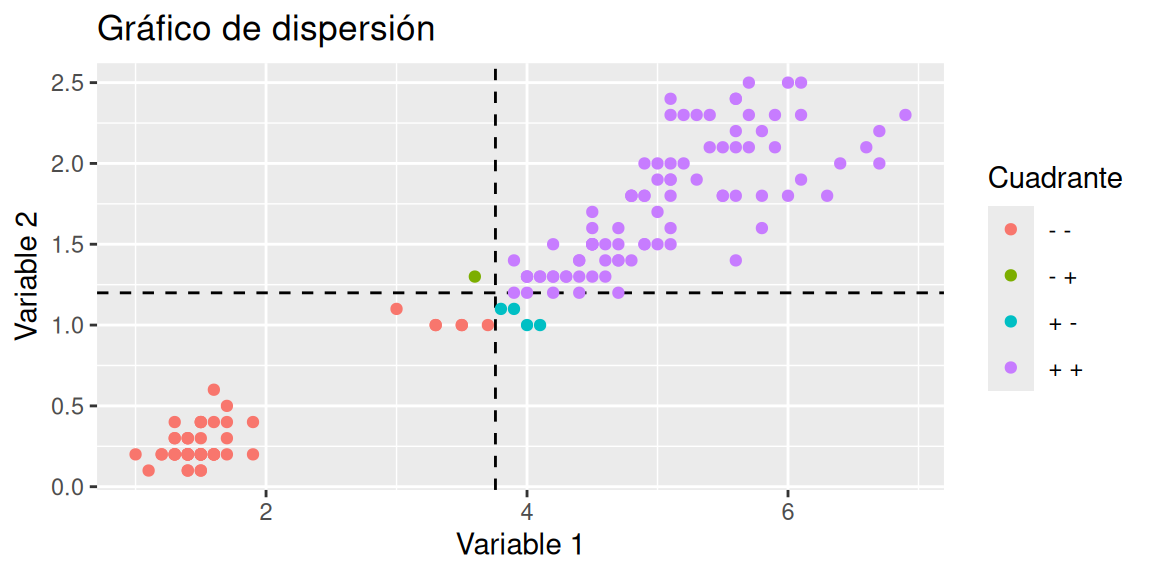
\includegraphics[width=\linewidth]{est2+inferencia_files/figure-latex/unnamed-chunk-87-1} \end{center}

En este caso, la mayoría de los puntos están en los cuadrantes `\(+ +\)' y `\(- -\)', y en estos cuadrantes la expresión \((x_i-\bar{x})(y_i-\bar{y})\) es positiva; por eso la covarianza es positiva (aunque también necesario considerar que tan lejos están los puntos de la intersección de las líneas promedio). \textbf{¿Es pronunciada la relación lineal?}

\subsection{Correlación}\label{regresion-lineal-correlacion}

Aunque con el signo de la covarianza podemos detectar el tipo de relación entre dos variables, al depender de las unidades de \(X\) y de \(Y\), no sabemos si corresponde a un relación fuerte o débil (es decir, la forma lineal es fuertemente o débilmente pronunciada); sólo sabemos el signo. Para solucionar esto, \textbf{estandarizamos} los valores. La fórmula que realiza este proceso utilizando la covarianza es

\begin{equation}
r_{XY} = \frac{S_{XY}}{S_{X}S_{Y}}
\label{eq:Correlacion}
\end{equation}

Este estadístico, también conocido como \textbf{Coeficiente de correlación de Pearson} se encuentra entre -1 y 1.

\begin{itemize}
\item
  Si \(r_{XY} = 0\), entonces no hay relación lineal o con relación lineal débil entre las variables.
\item
  Si \(r_{XY}\) es cercano a 1, entonces hay relación lineal directa y fuerte entre variables.
\item
  Si \(r_{XY}\) es cercano a \(-1\), entonces hay relación lineal inversa y fuerte entre las variables.
\end{itemize}

Una regla más fina sobre la intensidad de la relación es \citep{ratner_correlation_2009}:

\begin{itemize}
\tightlist
\item
  \(r_{XY} = 0\) indica que no hay relación lineal.
\item
  \(r_{XY} = 1\) indica una relación lineal positiva perfecta: a medida que una variable aumenta en sus valores, la otra variable también aumenta en sus valores a través de una regla lineal exacta.
\item
  \(r_{XY} = -1\) indica una relación lineal negativa perfecta: a medida que una variable aumenta en sus valores, la otra variable disminuye en sus valores a través de una regla lineal exacta.
\item
  Los valores entre \(0\) y \(0.3\) (\(0\) y \(−0.3\)) indican una relación lineal positiva (negativa) débil a través de una regla lineal inestable.
\item
  Valores entre \(0.3\) y \(0.7\) (\(-0.3\) y \(−0.7\)) indican una relación lineal positiva (negativa) moderada a través de una regla lineal difusa-firme.
\item
  Los valores entre \(0.7\) y \(1.0\) (\(−0.7\) y \(−1.0\)) indican una fuerte relación lineal positiva (negativa) a través de una regla lineal firme.
\end{itemize}

\begin{exercise}
Por ejemplo, si \(r_{XY} = -0.96\), ¿qué podemos decir acerca de la relación entre \(X\) e \(Y\)?
\end{exercise}

A continuación, se estudia gráficamente la correlación entre dos variables. Para ello, se necesita del gráfico de dispersión y una recta que refleje la asociación lineal (detalles de esta recta en secciones posteriores).

\begin{center}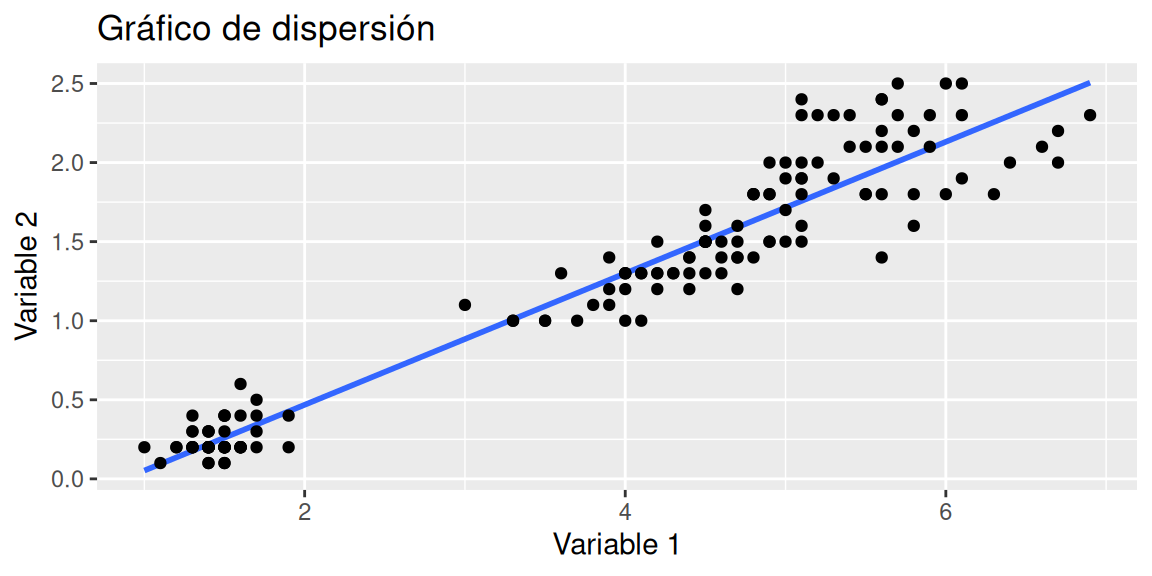
\includegraphics[width=\linewidth]{est2+inferencia_files/figure-latex/unnamed-chunk-88-1} \end{center}

\textbf{Nota:} En R, se utiliza el comando \texttt{cor()} para calcular la correlación entre dos variables.

\textbf{¿Cómo se comportan los puntos al rededor de la línea azul?}

\begin{exercise}

La base de datos \href{https://raw.githubusercontent.com/Dfranzani/Bases-de-datos-para-cursos/main/2022-2/Estad\%C3\%ADstica\%202/dolar.csv}{\emph{graficos+dolar.csv}} contiene el valor del dólar observado de algunos de los días de los meses de junio y julio del 2022, tomados por el el SII. A continuación:

\begin{enumerate}
\def\labelenumi{\arabic{enumi}.}
\tightlist
\item
  Realice un histograma del valor de dólar.
\item
  Realice un histograma del valor de dólar diferenciado por mes. Utilice el comando \texttt{facet\_grid(\textasciitilde{}Mes)}.
\item
  Reordene los gráficos por mes. Para ello convierta la variable Mes a factor, ordenando los meses como corresponde.
\item
  Realice un gráfico de Violín con caja y promedio del valor de dolar. Interprete lo observado.
\item
  Separe el gráfico anterior por mes. Comente lo observado.
\item
  Estudie las medidas de asociación entre los valores del dólar de los primeros 18 registros de cada mes. Interprete. ¿Por qué no es posible comparar todos los registros de cada uno de los meses?
\item
  Realice un gráfico de dispersión de los para estudiar las medidas de asociación entre las variables de la pregunta 6.
\end{enumerate}

\end{exercise}

\section{Regresión lineal simple}\label{regresion-lineal-simple}

La regresión lineal simple (RLS) consiste en generar un \textbf{modelo de regresión} (ecuación de una recta) que permita explicar la relación lineal que existe entre dos variables. A la variable dependiente, predicha o respuesta se le identifica como \(Y\) y a la variable predictora o independiente como \(X\). \citep[página 450]{Devore}

El modelo de regresión lineal simple se describe de acuerdo a la ecuación:

\begin{equation}
Y_i = \beta_0 + \beta_1X_i + \varepsilon_i \text{ , }i = 1,\ldots ,n \text{ , } \varepsilon_i \overset{\text{iid}}{\sim} N(0,\sigma^2)
\label{eq:regresion}
\end{equation}

Una ejemplificación de esta ecuación es la siguiente (\ref{fig:regresion1}).

\begin{figure}

{\centering 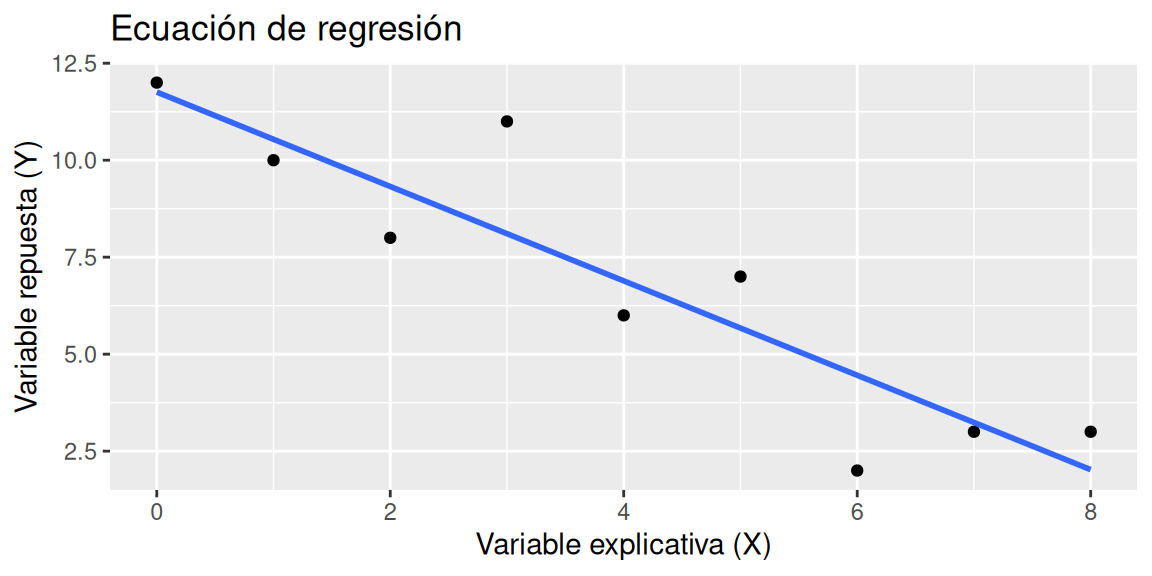
\includegraphics[width=\linewidth]{est2+inferencia_files/figure-latex/regresion1-1} 

}

\caption{Ecuación de regresión}\label{fig:regresion1}
\end{figure}

Siendo \(\beta_0\) la ordenada en el origen, \(\beta_1\) la pendiente y \(\varepsilon\) el \textbf{error aleatorio}. Este último representa la diferencia entre el valor ajustado por la recta y el valor real (línea de color rojo en el gráfico en la figura \ref{fig:regresion2}), el cual, recoge el efecto de todas aquellas variables que influyen en \(Y\) pero que no se incluyen en el modelo como predictores.

\begin{figure}

{\centering 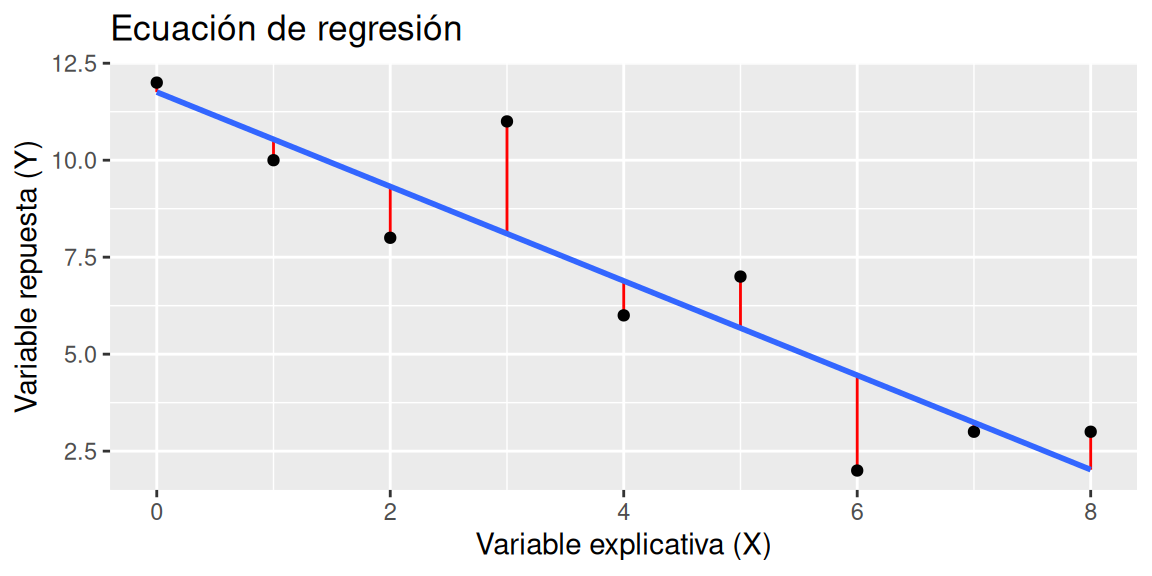
\includegraphics[width=\linewidth]{est2+inferencia_files/figure-latex/regresion2-1} 

}

\caption{Errores de una ecuación de regresión}\label{fig:regresion2}
\end{figure}

La ecuación \eqref{eq:regresion} representa la \textbf{ecuación de regresión verdadera} (o poblacional). Sin embargo, no es posible conocer el valor de \(\beta_0\) y \(\beta_1\), ya que son parámetros (de antemano, no se conocen todos los datos de la población), por lo cual, se determinan estimadores que permiten aproximar los valores de los parámetros a partir de una muestra, para así de determinar una ecuación de regresión estimada \eqref{eq:ecuacion-regresion-estimada}.

\begin{equation}
Y_i = \widehat{\beta}_0 + \widehat{\beta}_1X_i
\label{eq:ecuacion-regresion-estimada}
\end{equation}

\subsection{Estimadores de mínimos cuadrados}\label{EMCRLS}

Una forma intuitiva de abordar el problema de estimar \(\beta_0\) y \(\beta_1\) es minimizando los errores aleatorios. Para ello, se hace uso de la ecuación de regresión verdadera:

\[
Y_i = \beta_0 + \beta_1X_i + \varepsilon_i
\]

Luego, es posible escribir el error aleatorio de la siguiente manera:

\begin{equation}
\varepsilon_i = Y_i - [\beta_0 + \beta_1X_i]
\label{eq:funcion-errores}
\end{equation}

Para considerar el error en cada uno de los puntos al rededor de la recta de regresión verdadera se considera la suma de los errores. Sin embargo, para tener mayor facilidad en el proceso de determinar los estimadores, se elevan los errores al cuadrado (\textbf{suma cuadrática de errores}).

\begin{equation}
\sum_{i=1}^n\varepsilon_i^2 = \sum_{i=1}^n (Y_i - [\beta_0 + \beta_1X_i])^2
\label{eq:sumacuadratica-RL}
\end{equation}

Llegado a este punto, es natural minimizar esta función, ya que los valores de \(\beta_0\) y \(\beta_1\) estimados buscan dar lugar a la recta que ``pasa lo más cerca posible de todos los puntos''. Los estimadores de \(\beta_0\) y \(\beta_1\) se denotan por \(\widehat{\beta}_0\) y \(\widehat{\beta}_1\) respectivamente, y son denominados como \textbf{Estimadores de Mínimos Cuadrados} (EMC).

Los estimadores de \(\beta_0\) y \(\beta_1\) son (detalles del desarrollo en el anexo \ref{RLS-EMC}):

\begin{equation}
\widehat{\beta}_1 = \frac{\displaystyle\sum_{i=1}^n(x_i-\bar{x})(y_i-\bar{y})}{\displaystyle\sum_{i=1}^n(x_i-\bar{x})^2} = \frac{S_Y}{S_X}r_{XY}
\label{eq:beta1gorro}
\end{equation}

\begin{equation}
\widehat{\beta}_0 = \bar{y} - \widehat{\beta}_1\bar{x}
\label{eq:beta0gorro}
\end{equation}

\begin{itemize}
\tightlist
\item
  Los valores de \(S_y\) y \(S_x\) son las desviaciones estándar muestrales de cada variable y \(r_{XY}\) el coeficiente de correlación entre estas.
\item
  \(\widehat{\beta}_0\) es el valor esperado la variable \(Y\) cuando \(X = 0\), es decir, la intersección de la recta con el eje \(y\). En ocasiones, no tiene interpretación práctica (situaciones en las que \(X\) no puede adquirir el valor 0).
\item
  \(\widehat{\beta}_1\) corresponde al valor de la pendiente. La interpretación de este valor se detalla más adelante.
\item
  \(\widehat{Y}\) se entiende como el valor esperado, es decir, el valor promedio (muestral) de \(Y\).
\item
  La diferencia entre los valores reales \(Y\) (en la base de datos) y los valores de la recta estimada (\(\widehat{Y}\)) se denominan residuos, que se denotan por la letra \(e\). Estos se observan de la misma forma que los errores aleatorios (figura \ref{fig:regresion2}).
\end{itemize}

\begin{example}
\protect\hypertarget{exm:AFPUNO}{}\label{exm:AFPUNO}

El archivo \href{https://raw.githubusercontent.com/Dfranzani/Bases-de-datos-para-cursos/main/2022-2/Estad\%C3\%ADstica\%202/cuota\%2Bpatrimonio.csv}{\emph{cuota+patrimonio.csv}} contiene los valores cuota (pesos) y valor del patrimonio (miles de millones de pesos) de los primeros dos meses del año 2022 de la AFP UNO. En R:

\begin{enumerate}
\def\labelenumi{\arabic{enumi}.}
\tightlist
\item
  Realice un estudio inicial de los datos, elaborando un gráfico de violín + caja + promedio para cada una de las variables.
\end{enumerate}

Inspeccionamos la base de datos.

\begin{Shaded}
\begin{Highlighting}[]
\CommentTok{\# Cargue previamente la base de datos, guardándola con el nombre "datos"}
\FunctionTok{str}\NormalTok{(datos)}
\end{Highlighting}
\end{Shaded}

\begin{verbatim}
## 'data.frame':    59 obs. of  2 variables:
##  $ Valor.Cuota     : num  65594 65594 65356 65860 65813 ...
##  $ Valor.Patrimonio: num  186 186 185 187 187 ...
\end{verbatim}

Luego, realizamos el gráfico de violín con caja y promedio.

\begin{Shaded}
\begin{Highlighting}[]
\FunctionTok{ggplot}\NormalTok{(}\AttributeTok{data =}\NormalTok{ datos, }\FunctionTok{aes}\NormalTok{(}\AttributeTok{y =} \DecValTok{1}\NormalTok{, }\AttributeTok{x =}\NormalTok{ Valor.Cuota)) }\SpecialCharTok{+} 
  \FunctionTok{geom\_violin}\NormalTok{(}\AttributeTok{trim =}\NormalTok{ F) }\SpecialCharTok{+}
  \FunctionTok{geom\_boxplot}\NormalTok{(}\AttributeTok{width =} \FloatTok{0.1}\NormalTok{) }\SpecialCharTok{+}
\FunctionTok{stat\_summary}\NormalTok{(}\AttributeTok{fun =}\NormalTok{ mean, }\AttributeTok{color =} \StringTok{"red"}\NormalTok{, }\AttributeTok{geom =} \StringTok{"point"}\NormalTok{, }\AttributeTok{orientation =} \StringTok{"y"}\NormalTok{) }\SpecialCharTok{+}
  \FunctionTok{labs}\NormalTok{(}\AttributeTok{y =} \StringTok{""}\NormalTok{, }\AttributeTok{x =} \StringTok{"Pesos"}\NormalTok{, }\AttributeTok{title =} \StringTok{"Valor Cuota"}\NormalTok{)}
\end{Highlighting}
\end{Shaded}

\begin{center}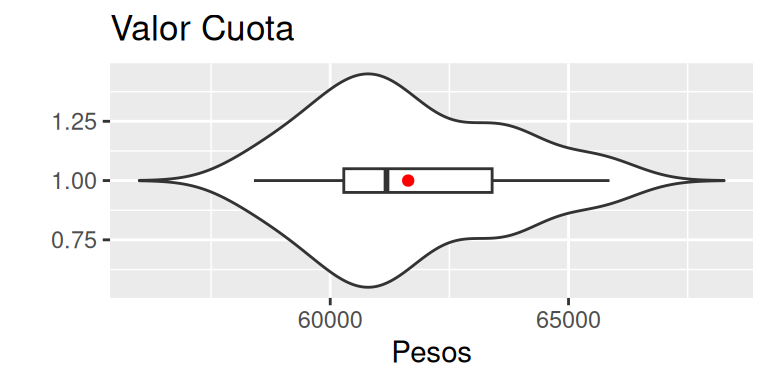
\includegraphics{est2+inferencia_files/figure-latex/unnamed-chunk-91-1} \end{center}

Se observa, que la mayor concentración de datos se encuentra entre el primer y segundo cuartil. Además, el cierre superior del gráfico de violín presenta una mayor concentración de datos que el cierre inferior, lo cual, explica la posición del promedio por sobre la mediana.

\begin{Shaded}
\begin{Highlighting}[]
\FunctionTok{ggplot}\NormalTok{(}\AttributeTok{data =}\NormalTok{ datos, }\FunctionTok{aes}\NormalTok{(}\AttributeTok{y =} \DecValTok{1}\NormalTok{, }\AttributeTok{x =}\NormalTok{ Valor.Patrimonio)) }\SpecialCharTok{+} 
  \FunctionTok{geom\_violin}\NormalTok{(}\AttributeTok{trim =}\NormalTok{ F) }\SpecialCharTok{+}
  \FunctionTok{geom\_boxplot}\NormalTok{(}\AttributeTok{width =} \FloatTok{0.1}\NormalTok{) }\SpecialCharTok{+}
\FunctionTok{stat\_summary}\NormalTok{(}\AttributeTok{fun =}\NormalTok{ mean, }\AttributeTok{color =} \StringTok{"red"}\NormalTok{, }\AttributeTok{geom =} \StringTok{"point"}\NormalTok{, }\AttributeTok{orientation =} \StringTok{"y"}\NormalTok{) }\SpecialCharTok{+}
  \FunctionTok{labs}\NormalTok{(}\AttributeTok{y =} \StringTok{""}\NormalTok{, }\AttributeTok{x =} \StringTok{"Miles de millones de pesos"}\NormalTok{, }\AttributeTok{title =} \StringTok{"Valor Patrimonio"}\NormalTok{)}
\end{Highlighting}
\end{Shaded}

\begin{center}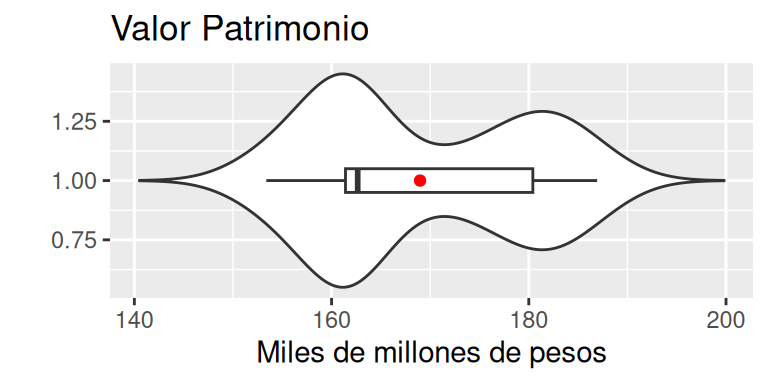
\includegraphics{est2+inferencia_files/figure-latex/unnamed-chunk-92-1} \end{center}

Se observa, que la mayor concentración de datos se encuentra entre el primer y segundo cuartil. Una segunda concentración se encuentra por sobre el tercer cuartil , lo cual, explica la posición del promedio por sobre la mediana.

\begin{enumerate}
\def\labelenumi{\arabic{enumi}.}
\setcounter{enumi}{1}
\tightlist
\item
  Estudie la correlación entre ambas variables.
\end{enumerate}

\begin{Shaded}
\begin{Highlighting}[]
\FunctionTok{cor}\NormalTok{(datos}\SpecialCharTok{$}\NormalTok{Valor.Cuota, datos}\SpecialCharTok{$}\NormalTok{Valor.Patrimonio)}
\end{Highlighting}
\end{Shaded}

\begin{verbatim}
## [1] 0.9218759
\end{verbatim}

El valor de la correlación indica que la relación lineal entre las dos variables es positiva y fuerte. Esto quiere decir que, cuando en promedio el valor cuota aumenta, el promedio el valor del patrimonio también aumenta.

\begin{enumerate}
\def\labelenumi{\arabic{enumi}.}
\setcounter{enumi}{2}
\tightlist
\item
  Considerando que desea explicar el valor del patrimonio a partir del valor cuota. Determine los valores de \(\widehat{\beta}_0\) y \(\widehat{\beta}_1\) utilizando el comando \texttt{lm()}.
\end{enumerate}

\begin{Shaded}
\begin{Highlighting}[]
\NormalTok{modelo }\OtherTok{=} \FunctionTok{lm}\NormalTok{(Valor.Patrimonio }\SpecialCharTok{\textasciitilde{}}\NormalTok{ Valor.Cuota, }\AttributeTok{data =}\NormalTok{ datos)}
\NormalTok{modelo}
\end{Highlighting}
\end{Shaded}

\begin{verbatim}
## 
## Call:
## lm(formula = Valor.Patrimonio ~ Valor.Cuota, data = datos)
## 
## Coefficients:
## (Intercept)  Valor.Cuota  
##  -1.353e+02    4.936e-03
\end{verbatim}

\begin{enumerate}
\def\labelenumi{\arabic{enumi}.}
\setcounter{enumi}{3}
\tightlist
\item
  Escriba la ecuación de la recta de regresión ajustada.
\end{enumerate}

\[
\widehat{Y}_i = -135.3 + 0.004936X_i
\]

\begin{enumerate}
\def\labelenumi{\arabic{enumi}.}
\setcounter{enumi}{4}
\tightlist
\item
  Realice un gráfico de la la recta de regresión y los residuos del modelo.
\end{enumerate}

\begin{Shaded}
\begin{Highlighting}[]
\CommentTok{\# Guardamos los valores de la recta estimada en una nueva columna en la base de datos}
\NormalTok{datos}\SpecialCharTok{$}\NormalTok{Ajustados }\OtherTok{=}\NormalTok{ modelo}\SpecialCharTok{$}\NormalTok{fitted.values}
\FunctionTok{ggplot}\NormalTok{(}\AttributeTok{data =}\NormalTok{ datos, }\FunctionTok{aes}\NormalTok{(}\AttributeTok{x =}\NormalTok{ Valor.Cuota, }\AttributeTok{y =}\NormalTok{ Valor.Patrimonio)) }\SpecialCharTok{+}
  \FunctionTok{geom\_segment}\NormalTok{(}\FunctionTok{aes}\NormalTok{(}\AttributeTok{x =}\NormalTok{ Valor.Cuota, }\AttributeTok{xend =}\NormalTok{ Valor.Cuota,}
                   \AttributeTok{y =}\NormalTok{ Valor.Patrimonio, }\AttributeTok{yend =}\NormalTok{ Ajustados), }\AttributeTok{color =} \StringTok{"red"}\NormalTok{) }\SpecialCharTok{+}
  \FunctionTok{labs}\NormalTok{(}\AttributeTok{x =} \StringTok{"Valor Cuota"}\NormalTok{, }\AttributeTok{y =} \StringTok{"Valor Patrimonio"}\NormalTok{,}
       \AttributeTok{title =} \StringTok{"Ecuación de regresión ajustada"}\NormalTok{) }\SpecialCharTok{+} 
  \FunctionTok{geom\_point}\NormalTok{() }\SpecialCharTok{+}
  \FunctionTok{geom\_smooth}\NormalTok{(}\AttributeTok{method =}\NormalTok{ lm, }\AttributeTok{se =} \ConstantTok{FALSE}\NormalTok{, }\AttributeTok{formula =} \StringTok{\textquotesingle{}y \textasciitilde{} x\textquotesingle{}}\NormalTok{)}
\end{Highlighting}
\end{Shaded}

\begin{center}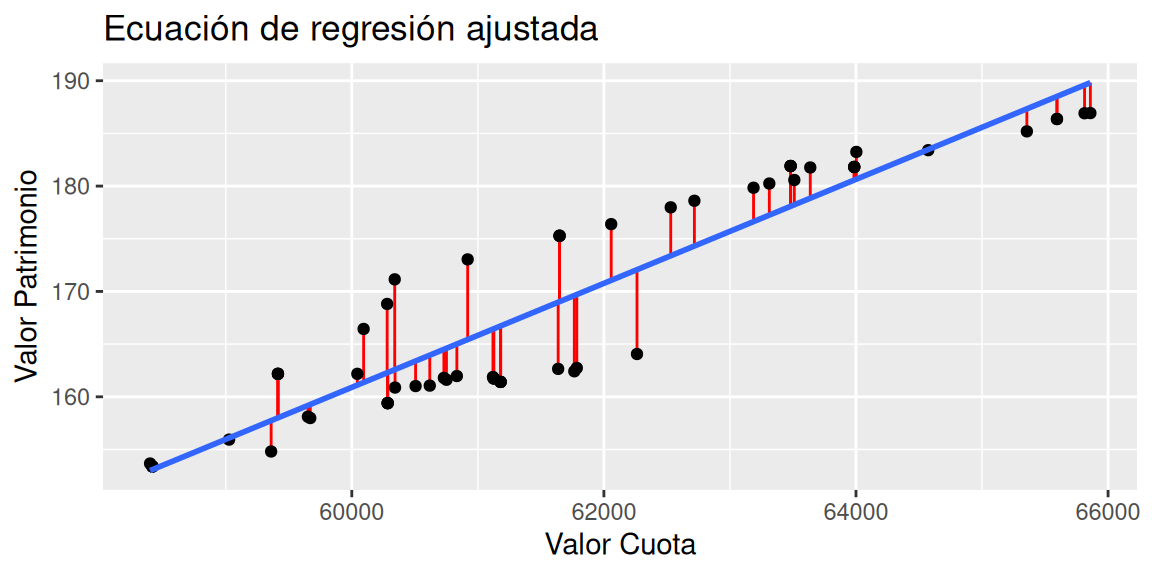
\includegraphics[width=\linewidth]{est2+inferencia_files/figure-latex/unnamed-chunk-95-1} \end{center}

\end{example}

Para interpretar cada uno de los beta estimados se debe hacer en función de la variable de estudio (variable dependiente). En este sentido,

\begin{itemize}
\item
  \(\widehat{\beta}_1\): corresponde a la pendiente de la ecuación de la recta de regresión ajustada, e indica un avance lineal constante en crecimiento o en decrecimiento dependiendo de su valor. La interpretación de este parámetro, está sujeta a la unidad de medida de la variable predictora \(X\), de tal manera, que una cambio en una unidad de medida de la variable \(x\), afecta en \textbf{promedio} \(\widehat{\beta}_1\) unidades en la variable \(Y\).

  En el ejemplo \ref{exm:AFPUNO}, el valor de \(\widehat{\beta}_1\) es de 0.004936 , lo cual indica que por cada unidad de valor cuota (por cada peso), el valor del patrimonio aumenta en promedio 0.004936 miles de millones pesos.
\item
  \(\widehat{\beta}_0\): es el intercepto de la ecuación de la recta de regresión ajustada, y se debe verificar que el valor obtenido tenga sentido con el fenómeno. En el ejemplo \ref{exm:AFPUNO}, se obtiene un valor lejano a cero (-135.2584663), por lo que, cuando \(\beta_1x\) vale cero (es decir, una cantidad de cuotas igual a 0), el valor del promedio del patrimonio es menor a cero. Esto tiene sentido, ya que las cuotas no constituyen la totalidad del valor del patrimonio de la AFP (en el ejemplo se trabaja con un fondo en específico de los cinco existentes, de un determinado producto de inversión).
\end{itemize}

\begin{exercise}
\protect\hypertarget{exr:ingreso}{}\label{exr:ingreso}

Utilizando la base de datos \hyperref[Ingreso]{Ingreso}:

\begin{enumerate}
\def\labelenumi{\arabic{enumi}.}
\tightlist
\item
  Realice un estudio inicial de los datos, elaborando un gráfico de violín + caja + promedio para cada una de las variables cuantitativas continuas, mientras que para las variables categóricas elabore tablas de frecuencias relativas.
\item
  Considerando que desea explicar la proporción de logro en el diagnóstico de comunicación escrita a partir del puntaje en la PTU de Lenguaje (considere esto para las siguientes preguntas), estudie la correlación entre ambas variables.
\item
  Determine los valores de \(\widehat{\beta}_0\) y \(\widehat{\beta}_1\) utilizando el comando \texttt{lm()}. Interprete los valores.
\item
  Escriba la ecuación de la recta de regresión ajustada.
\item
  Realice un gráfico de la la recta de regresión ajustada y los residuos del modelo.
\end{enumerate}

\end{exercise}

\subsection{Sumas cuadráticas}\label{sumascuadraticas}

En un modelo sin variables independientes los valores ajustados o predichos son iguales al promedio de las observaciones, \(\bar{Y}\) (tal como se mostró en la interpretación asociada a las estimaciones de los parámetros). Los residuos de dicho modelo corresponden a \(Y_i - \bar{Y}\). La \textbf{suma de cuadrados total} (SCT) se define como:

\begin{equation}
\text{SCT} = \sum_{i=1}^n\left( Y_i - \bar{Y} \right)^2
\label{eq:SCT}
\end{equation}

¿Cómo se relacionan la SCT y la suma cuadrática de errores (SCE)? Consideremos la siguiente igualdad.

\begin{equation}
Y_i - \bar{Y} = \left( \widehat{Y}_i - \bar{Y} \right) + \left( Y_i - \widehat{Y}_i \right)
\label{eq:SCT-SCE-SCReg}
\end{equation}

A partir de esta igualdad se demuestra que:

\begin{equation}
\underbrace{\sum_{i=1}^n\left( Y_i - \bar{Y} \right)^2}_{\text{SCT}} = \underbrace{\sum_{i=1}^n\left( \widehat{Y}_i - \bar{Y} \right)^2}_{\text{SCReg}} + \underbrace{\sum_{i=1}^n\left( Y_i - \widehat{Y}_i \right)^2}_{\text{SCE}},
\label{eq:descomposicion-sct}
\end{equation}

donde,

\begin{itemize}
\item
  \textbf{Suma de cuadrados total} (SCT): corresponde a la variabilidad de los datos.
\item
  \textbf{Suma de cuadrados de la regresión} (SCReg): corresponde a la variabilidad de los datos que es explicada por el modelo de regresión.
\item
  \textbf{Suma de cuadrados del error} (SCE): corresponde a la variabilidad de los datos que no es explicada por el modelo.
\end{itemize}

En la experimentación, se quiere que SCE sea pequeña y que SCReg sea grande.

Las expresiones involucradas en la ecuación \eqref{eq:descomposicion-sct} dan lugar a reescribir distintas expresiones, entre las cuales se encuentra, el coeficiente de determinación (\(R^2\)) y el error estándar residual explicados en la sección \ref{metricasRLS}, y el estadístico asociado a las pruebas de hipótesis de los parámetros explicado en la sección \ref{pruebasHipotesisRLS}.

\subsection{Pruebas de hipótesis}\label{pruebasHipotesisRLS}

Los modelos de regresión lineal simple incluyen pruebas de hipótesis asociadas a los betas, además de otro tipo de información. En R es posible utilizar el comando \texttt{summary()} para acceder al resumen de información. A continuación, a modo de ejemplo se utiliza el modelo elaborado en el ejemplo \ref{exm:AFPUNO}.

\begin{Shaded}
\begin{Highlighting}[]
\FunctionTok{summary}\NormalTok{(modelo)}
\end{Highlighting}
\end{Shaded}

\begin{verbatim}
## 
## Call:
## lm(formula = Valor.Patrimonio ~ Valor.Cuota, data = datos)
## 
## Residuals:
##     Min      1Q  Median      3Q     Max 
## -8.0070 -2.9085 -0.0636  3.8231  8.5680 
## 
## Coefficients:
##               Estimate Std. Error t value Pr(>|t|)    
## (Intercept) -1.353e+02  1.695e+01  -7.982 7.37e-11 ***
## Valor.Cuota  4.936e-03  2.748e-04  17.962  < 2e-16 ***
## ---
## Signif. codes:  0 '***' 0.001 '**' 0.01 '*' 0.05 '.' 0.1 ' ' 1
## 
## Residual standard error: 4.215 on 57 degrees of freedom
## Multiple R-squared:  0.8499, Adjusted R-squared:  0.8472 
## F-statistic: 322.6 on 1 and 57 DF,  p-value: < 2.2e-16
\end{verbatim}

El detalle por columna es el siguiente.

\begin{itemize}
\item
  En primer lugar, ya conocemos los coeficientes del modelo (betas estimados) y cómo se interpretan. Estos valores los podemos encontrar en la columna llamada \textbf{Estimate}.
\item
  La segunda columna (\textbf{Std. Error}) corresponde a la desviación estándar de la estimación de cada uno de los betas. Como cada uno de los errores (\(\varepsilon_i\)) tiene distribución normal, esto implica que cada uno de los \(\beta\) tenga distribución t -- Student (no analizaremos esto en profundidad).
\item
  La tercera y cuarta columna están diseñadas para probar una determinada prueba de hipótesis relacionada a los \(\beta\), llamada \textbf{prueba de no nulidad}. En este caso, cada fila aborda la siguiente hipótesis:

  \begin{equation}
  \notag
  \begin{split}
  H_0:&\beta_i = 0\\
  H_1:&\beta_i \neq 0\\
  \end{split}
  \end{equation}

  El estadístico para cada uno de los beta se obtiene dividiendo el valor estimado (\textbf{Estimate}) por la desviación estándar (\textbf{Std. Error}). El resultado de estos valores, se puede apreciar en la columna \textbf{t value}.
\item
  Finalmente, se calcula el valor - p asociado a cada una de las hipótesis del punto anterior, con la fórmula \(2\cdot(1-pt(|t_0|, n-2))\). El valor resultante de esta expresión para cada uno de los betas se encuentra en la columna \textbf{Pr(\textgreater\textbar t\textbar)}. La interpretación de este valor es mediante el criterio del valor - p presentado en la unidad anterior.
\end{itemize}

En el ejemplo \ref{exm:AFPUNO}, al no rechazarse la hipótesis nula asociada a cada beta estimado, se tiene que cada variable (intercepto y valor cuota) son relevantes para explicar la variable respuesta (valor del patrimonio). Sin embargo, esto no es un regla decidora respecto a si una variable debe o no considerarse en el modelo, es decir,

\begin{itemize}
\item
  No rechazar las hipótesis nula de los beta estimados, indica que su ``valor'' es \textbf{cero}, por lo que no ``aportarían'' al modelo de regresión construido. En este punto, muchas personas eliminarían la variable utilizada para construir el modelo (el valor cuota) (esto es una de tantas técnicas aplicables, pero que no profundizaremos) o, cambiarían la variable explicativa utilizada (no considerarían el valor cuota, sino que utilizarían otra variable).
\item
  A pesar de que los valores-p puedan no ser significativos (mayores a 0.05), es decir, no rechazar las hipótesis nulas; es posible forzar la permanencia de la variable en el modelo debido al criterio experto del profesional.
\end{itemize}

Por último, al final de la salida del resumen, encontramos el valor llamado \textbf{F-statistic}. Este valor, es un estadístico que prueba de hipótesis llamada \textbf{prueba de no nulidad conjunta},

\begin{equation}
\notag
\begin{split}
H_0:&\text{ Todos los betas asociados a las covariables valen 0}\\
H_1:&\text{ Almenos uno de los betas asociados a las covariables es distinto de 0}\\
\end{split}
\end{equation}

Se rechaza \(H_0\) cuando:

\begin{equation}
F_0 = \frac{\text{SCReg}}{\text{MCE}} \geq F_{1-\alpha, 1, n-2}.
\label{eq:estadistico-F-RLS}
\end{equation}

con una significancia \(\alpha\). El valor de MCE se especifica en la sección \ref{metricasRLS}.

\textbf{Nota}: esta prueba de hipótesis no considera \(\beta_0\).

En el ejemplo \ref{exm:AFPUNO}, se observa un valor del estadístico igual a 322.6 con 1 y 57 grados de libertad, además de un valor menor a 0.05. Por lo tanto, existe suficiente evidencia estadística para rechazar \(H_0\), es decir, almenos uno de los betas asociados a las covariables es distinto de 0.

\begin{exercise}

Utilizando la base de datos \hyperref[Pacientes]{Pacientes}:

\begin{enumerate}
\def\labelenumi{\arabic{enumi}.}
\tightlist
\item
  Ajuste un modelo para estudiar el nivel de colesterol de los pacientes a partir de su edad. Luego, estudie las pruebas de hipótesis asociadas utilizando una confianza del 95\%.
\item
  Ajuste un modelo para estudiar el tiempo de duración del último ataque al corazón de los pacientes a partir de su edad. Luego, estudie las pruebas de hipótesis asociadas utilizando una confianza del 95\%.
\end{enumerate}

\end{exercise}

\subsection{Métricas}\label{metricasRLS}

La salida de R nos proporciona dos valores que permiten evaluar al modelo de regresión lineal simple:

\begin{itemize}
\item
  \textbf{Residual standard error} (error estándar residual): corresponde a la desviación estándar de los residuos, es decir, que mientras menor sea este valor, los puntos se alejarán menos de la recta de regresión. Este valor es una estimación de \(\sigma\), que en términos de las expresiones de la ecuación \eqref{eq:descomposicion-sct} se tiene que:

  \begin{equation}
  \widehat{\sigma}^2 = \frac{\text{SCE}}{n-2} = \text{MCE},
  \label{eq:sigma2-estimador}
  \end{equation}

  donde, MCE se denomina \textbf{media cuadrática del error}. El denominador de esta expresión corresponde al total de observaciones (\(n\)) menos la cantidad de parámetros del modelo (\(\beta_1\) y \(\beta_2\)). Finalmente, el valor del error estándar residual (\(\widehat{\sigma}\)) es igual a \(\sqrt{\text{MCE}}\).
\item
  \textbf{Multiple R-squared} o \(R^2\): es un métrica de error de la regresión que mide el rendimiento del modelo, corresponde a la proporción de variabilidad explicada por la regresión sobre la variabilidad total de las observaciones. En términos de las expresiones de la ecuación \eqref{eq:descomposicion-sct} se tiene que:

  \begin{equation}
  R^2 = \frac{\text{SCReg}}{\text{SCT}}
  \label{eq:R2-RLS}
  \end{equation}
\end{itemize}

En el ejemplo \ref{exm:AFPUNO} se obtiene un error estándar residual de 4.2. Sin embargo, \textbf{NO EXISTE} un regla que determine cuando un error estándar residual es bueno o malo. En general, este valor se utiliza para comparar don o más modelos que estudian la misma variable respuesta pero con distintas variables predictoras (variables independientes), para saber cual realiza un mejor ajuste.

Por otro lado, se tiene un valor de \(R^2\) igual a 0.84, el cual es muy alto, por lo que se logra explicar gran parte de la variable respuesta. Al igual que el error estándar residual, no existe una regla para determinar cuando un valor de \(R^2\) es bueno o malo, aunque valores cercanos a cero indican que el poder explicativo del modelo es extremadamente pobre; y a su vez, valores muy cercanos a 1 son muy buenos, aunque extremadamente sospechosos.

Lo anteriormente explicado se puede observar mediante los siguientes comandos, aunque es posible observarlos en salida general del comando \texttt{summary()}.

\begin{Shaded}
\begin{Highlighting}[]
\CommentTok{\# Resumen del modelo}
\NormalTok{summ }\OtherTok{=} \FunctionTok{summary}\NormalTok{(modelo)}
\FunctionTok{print}\NormalTok{(}\FunctionTok{c}\NormalTok{(}\StringTok{"Error estándar residual"} \OtherTok{=}\NormalTok{ summ}\SpecialCharTok{$}\NormalTok{sigma, }\StringTok{"R cuadrado"} \OtherTok{=}\NormalTok{ summ}\SpecialCharTok{$}\NormalTok{r.squared))}
\end{Highlighting}
\end{Shaded}

\begin{verbatim}
## Error estándar residual              R cuadrado 
##               4.2148482               0.8498553
\end{verbatim}

\begin{exercise}

Utilizando la base de datos \hyperref[Ingreso]{Ingreso}:

\begin{enumerate}
\def\labelenumi{\arabic{enumi}.}
\tightlist
\item
  Ajuste un modelo para estudiar la proporción de logro a partir el puntaje NEM.
\item
  Ajuste un modelo para estudiar la proporción de logro a partir el puntaje PTU de la prueba de Lenguaje.
\item
  Obtenga de manera manual el estadístico F asociado a la prueba de hipótesis de nulidad conjunta de cada modelo. Interprete, utilizando una confianza del 95\%.
\item
  Compare los ajustes de ambos modelos utilizando el error estándar residual y el \(R^2\), obteniendo las métricas de manera manual. Interprete.
\end{enumerate}

\end{exercise}

\subsection{Supuestos}\label{regresion-lineal-simple-supuestos}

Cuándo se elabora un modelo de regresión lineal, es necesario verificar el cumplimiento de condiciones para la correcta interpretación y utilización del modelo desarrollado. Las condiciones que se deben cumplir se denominan supuestos. A continuación, se detallan los 4 supuestos que se deben estudiar, utilizando como ejemplo el modelo elaborado en el ejemplo \ref{exm:AFPUNO}.

\subsubsection{Linealidad}\label{regresion-lineal-simple-supuestos-linealidad}

La relación entre ambas variables (dependiente e independiente) debe ser lineal. Para observar el comportamiento es posible realizar un gráfico de puntos entre la variable predictora (\(X\)) y la variable de estudio (\(Y\)).

\begin{Shaded}
\begin{Highlighting}[]
\FunctionTok{ggplot}\NormalTok{(}\AttributeTok{data =}\NormalTok{ datos) }\SpecialCharTok{+}
  \FunctionTok{geom\_point}\NormalTok{(}\FunctionTok{aes}\NormalTok{(}\AttributeTok{x =}\NormalTok{ Valor.Cuota, }\AttributeTok{y =}\NormalTok{ Valor.Patrimonio)) }\SpecialCharTok{+}
  \FunctionTok{labs}\NormalTok{(}\AttributeTok{x =} \StringTok{"Valor Cuota (pesos)"}\NormalTok{, }\AttributeTok{y =} \StringTok{"Valor Patrimonio }\SpecialCharTok{\textbackslash{}n}\StringTok{ (miles de millones de pesos)"}\NormalTok{)}
\end{Highlighting}
\end{Shaded}

\begin{center}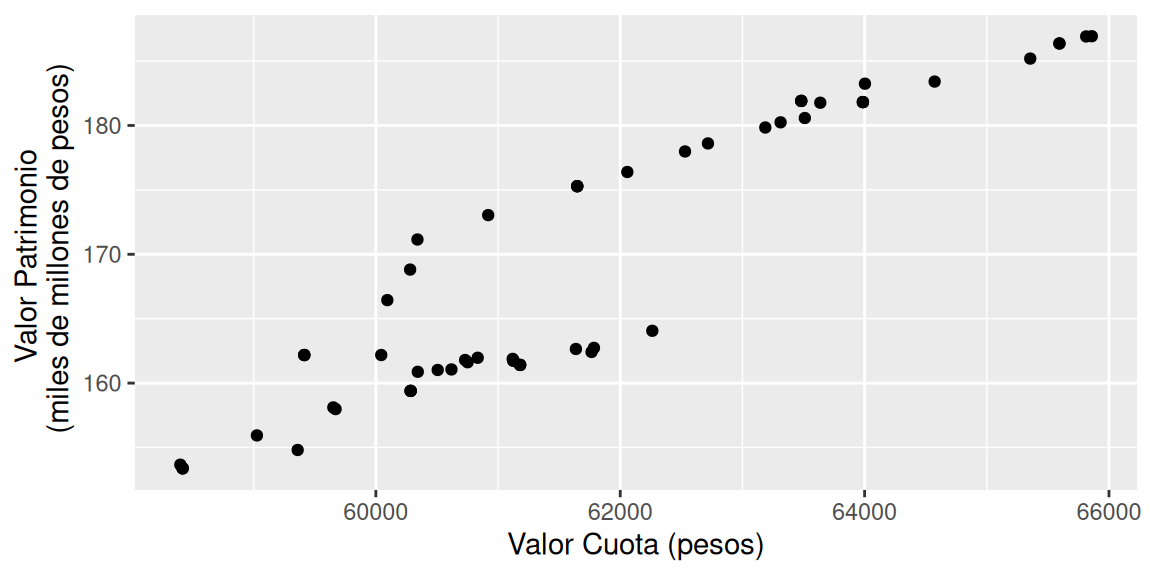
\includegraphics[width=\linewidth]{est2+inferencia_files/figure-latex/unnamed-chunk-98-1} \end{center}

La interpretación del comportamiento queda a discreción del profesional. En este caso, se aprecia una clara tendencia lineal, por lo que se asume que se cumple el supuesto de linealidad.

\subsubsection{Normalidad}\label{regresion-lineal-simple-supuestos-normalidad}

Los residuos \texttt{estandarizados} deben distribuir Normal con media 0 (\(\mu\)) y varianza 1 (\(\sigma^2\)). Para ello, se pueden ejecutar varios comandos en R para probar esta hipótesis. El más conocido es el comando \texttt{shapiro.test()}. La hipótesis es

\begin{equation}
\notag
\begin{split}
H_0&: \text{Los residuos estandarizados tienen distribución Normal}\\
H_1&: \text{Los residuos estandarizados NO tienen distribución Normal}\\
\end{split}
\end{equation}

Se definen los residuos estandarizados, \(r_i\), como los residuos, \(e_i\), divididos por su error estándar:

\begin{equation}
r_i = \frac{e_i}{\widehat{\text{es}}(e_i)}, i = 1,\ldots,n
\label{eq:residuos-estandarizados}
\end{equation}

Utilizando la definición dada en la ecuación \eqref{eq:sigma2-estimador}, se tiene que

\begin{equation}
r_i = \frac{e_i}{\sqrt{\text{MCE}}}
\label{eq:residuos-estandarizados-2}
\end{equation}

\begin{Shaded}
\begin{Highlighting}[]
\NormalTok{residuos }\OtherTok{=} \FunctionTok{resid}\NormalTok{(modelo) }\CommentTok{\# Residuos }
\NormalTok{residuos\_estandarizados }\OtherTok{=} \FunctionTok{rstandard}\NormalTok{(modelo) }\CommentTok{\# Residuos estandarizados}
\FunctionTok{shapiro.test}\NormalTok{(}\AttributeTok{x =}\NormalTok{ residuos\_estandarizados)}
\end{Highlighting}
\end{Shaded}

\begin{verbatim}
## 
##  Shapiro-Wilk normality test
## 
## data:  residuos_estandarizados
## W = 0.96765, p-value = 0.1177
\end{verbatim}

Considerando una confianza del 95\%, el valor-p de 0.1177 no es menor o igual a la significancia de 0.05, por lo cual, no existe suficiente evidencia estadística para rechazar la hipótesis nula, es decir, se asume que los residuos (estandarizados) tienen distribución normal.

En caso de que la cantidad de datos sea mayor a 5000, el comando \texttt{shapiro.test()} fallará. En su lugar, es posible usar el comando \texttt{ks.test()}, un ejemplo con los residuos del ejemplo anterior es

\begin{Shaded}
\begin{Highlighting}[]
\FunctionTok{ks.test}\NormalTok{(residuos\_estandarizados, }\StringTok{"pnorm"}\NormalTok{, }\DecValTok{0}\NormalTok{, }\DecValTok{1}\NormalTok{)}
\end{Highlighting}
\end{Shaded}

\begin{verbatim}
## 
##  Asymptotic one-sample Kolmogorov-Smirnov test
## 
## data:  residuos_estandarizados
## D = 0.12515, p-value = 0.3138
## alternative hypothesis: two-sided
\end{verbatim}

Una tercera opción es utilizar el comando \texttt{ad.test()} de la librería \textbf{nortest}

\begin{Shaded}
\begin{Highlighting}[]
\FunctionTok{library}\NormalTok{(nortest)}
\FunctionTok{ad.test}\NormalTok{(residuos\_estandarizados)}
\end{Highlighting}
\end{Shaded}

\begin{verbatim}
## 
##  Anderson-Darling normality test
## 
## data:  residuos_estandarizados
## A = 0.71269, p-value = 0.05962
\end{verbatim}

\subsubsection{Homocedasticidad}\label{regresion-lineal-simple-supuestos-homocedasticidad}

Este supuesto hace referencia a la necesidad de una varianza constante de los residuos. Para verificar esto, se grafican los residuos estandarizados del modelo versus los valores de la variable predictora (o variable predicha, \(\widehat{y}\)). Se busca que las amplitudes verticales en las figuras sean similares en la medida que se recorre el eje de las abscisas. Similarmente, es posible ejecutar una prueba de hipótesis (Breucsh - Pagan) en R con el comando \texttt{bptest()} de la librería \textbf{lmtest}, siendo

\begin{equation}
\notag
\begin{split}
H_0&: \text{Los residuos tienen varianza constante}\\
H_1&: \text{Los residuos NO tienen varianza constante}\\
\end{split}
\end{equation}

\begin{Shaded}
\begin{Highlighting}[]
\NormalTok{valores\_predichos }\OtherTok{=}\NormalTok{ modelo}\SpecialCharTok{$}\NormalTok{fitted.values}
\FunctionTok{ggplot}\NormalTok{(}\AttributeTok{data =}\NormalTok{ datos) }\SpecialCharTok{+}
  \FunctionTok{geom\_point}\NormalTok{(}\FunctionTok{aes}\NormalTok{(}\AttributeTok{x =}\NormalTok{ valores\_predichos,}
                 \AttributeTok{y =}\NormalTok{ residuos\_estandarizados)) }\SpecialCharTok{+}
  \FunctionTok{geom\_hline}\NormalTok{(}\AttributeTok{yintercept =} \DecValTok{0}\NormalTok{) }\SpecialCharTok{+}
  \FunctionTok{labs}\NormalTok{(}\AttributeTok{x =} \StringTok{"Valores predichos"}\NormalTok{, }\AttributeTok{y  =} \StringTok{"Residuos estandarizados"}\NormalTok{)}
\end{Highlighting}
\end{Shaded}

\begin{center}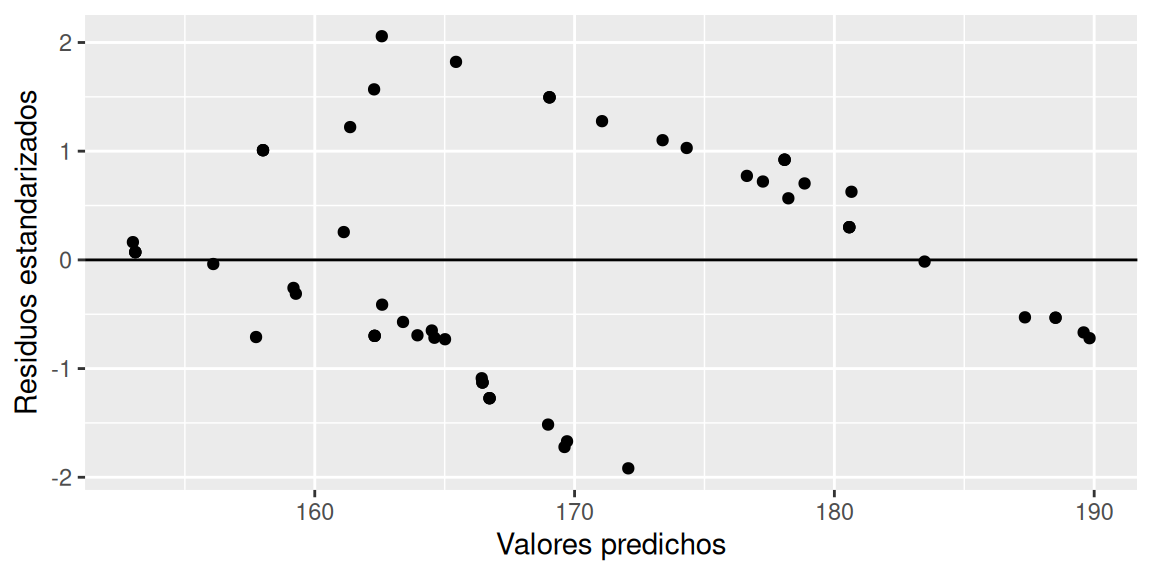
\includegraphics[width=\linewidth]{est2+inferencia_files/figure-latex/unnamed-chunk-102-1} \end{center}

Las amplitudes verticales no tiene un patrón claro de cambio (puede ser difícil de interpretar), por lo que utilizaremos la prueba de Breucsh - Pagan para decidir.

\begin{Shaded}
\begin{Highlighting}[]
\FunctionTok{library}\NormalTok{(lmtest)}
\FunctionTok{bptest}\NormalTok{(}\AttributeTok{formula =}\NormalTok{ Valor.Patrimonio }\SpecialCharTok{\textasciitilde{}}\NormalTok{ Valor.Cuota,}
       \AttributeTok{data =}\NormalTok{ datos)}
\end{Highlighting}
\end{Shaded}

\begin{verbatim}
## 
##  studentized Breusch-Pagan test
## 
## data:  Valor.Patrimonio ~ Valor.Cuota
## BP = 0.30064, df = 1, p-value = 0.5835
\end{verbatim}

Considerando una confianza del 95\%, el valor-p de 0.5835 no es menor o igual a la significancia de 0.05, por lo cual, no existe suficiente evidencia estadística para rechazar la hipótesis nula, es decir, se asume que los residuos tienen varianza constante (homocedasticidad).

\subsubsection{Independencia}\label{regresion-lineal-simple-supuestos-independencia}

El último supuesto corresponde a la independencia de los residuos, es decir que, no deben estar correlacionados entre ellos (autocorrelación igual a 0). La prueba de hipótesis de Durbin - Watson está diseñada para detectar autocorrelación en los residuos. Para ejecutar esta prueba en R se debe utilizar la función \texttt{dwtest()} de la librería \textbf{lmtest}. La hipótesis es

\begin{equation}
\notag
\begin{split}
H_0&: \text{Autocorrelación de los residuos es igual a 0}\\
H_1&: \text{Autocorrelación de los residuos es distinta de 0}\\
\end{split}
\end{equation}

\begin{Shaded}
\begin{Highlighting}[]
\CommentTok{\# Prueba de Durbin Watson}
\FunctionTok{dwtest}\NormalTok{(}\AttributeTok{formula =}\NormalTok{ Valor.Patrimonio }\SpecialCharTok{\textasciitilde{}}\NormalTok{ Valor.Cuota,}
       \AttributeTok{data =}\NormalTok{ datos,}
       \AttributeTok{alternative =} \StringTok{"two.sided"}\NormalTok{)}
\end{Highlighting}
\end{Shaded}

\begin{verbatim}
## 
##  Durbin-Watson test
## 
## data:  Valor.Patrimonio ~ Valor.Cuota
## DW = 0.080415, p-value < 2.2e-16
## alternative hypothesis: true autocorrelation is not 0
\end{verbatim}

Considerando una confianza del 95\%, el valor-p de \(2.2 \times 10^{-16}\) es menor o igual a la significancia de 0.05, por lo cual, existe suficiente evidencia estadística para rechazar la hipótesis nula, es decir, se asume que los residuos no son independientes (autocorrelación distinta de 0).

\textbf{Conclusión}: En resumen, se han cumplido 3 de los 4 supuestos planteados. Esto es muy común que suceda en la realidad, además de existir diversos factores que influyen en los resultados vistos.

\begin{exercise}

Utilizando la base de datos \hyperref[Ingreso]{Ingreso}, ajuste el modelo:

\[\widehat{Y}_{\text{Logro}} = \widehat{\beta}_0 + \widehat{\beta}_1X_{\text{NEM}}\]
Luego,

\begin{enumerate}
\def\labelenumi{\arabic{enumi}.}
\tightlist
\item
  Escriba la ecuación de regresión ajustada.
\item
  Verifique los supuestos del modelo, utilizando una confianza del 95\% cuando corresponda.
\end{enumerate}

\end{exercise}

\begin{exercise}
Utilizando la base de datos \hyperref[Pacientes]{Pacientes}, elabore un modelo para estudiar la variable \emph{oldpeak} a través de la variable \emph{chol}. Estudie los supuestos del modelo, utilizando una confianza del 92\%.
\end{exercise}

\begin{exercise}

La base de datos \href{https://raw.githubusercontent.com/Dfranzani/Bases-de-datos-para-cursos/main/2022-2/Estad\%C3\%ADstica\%202/terremotos.csv}{\emph{terremotos.csv}}, contiene datos sobre los terremotos ocurridos a nivel mundial entre los años 1900 y 2014. Las columnas de la base de datos son:

\begin{itemize}
\tightlist
\item
  Ano: año de ocurrencia del terremoto.
\item
  Latitud: grados decimales de la coordenada de latitud (valores negativos para latitudes del sur).
\item
  Longitud: grados decimales de la coordenada de longitud (valores negativos para longitudes occidentales).
\item
  Profundidad: profundidad del evento en kilómetros.
\item
  Magnitud: magnitud del evento (la escala no es fija, ya que, a través de los años, la escala a cambiado según el método de medición. Sin embargo, todos las magnitudes son comparables, indicando que a mayor magnitud, mayor es la intensidad en movimiento/fuerza del terremoto).
\end{itemize}

Ajuste los siguientes modelos:

\begin{itemize}
\item
  \(Y_{\text{Magnitud}} = \beta_0 + \beta_1X_{\text{Profundidad}} + \varepsilon, \varepsilon_i \overset{\text{iid}}{\sim} N(0,\sigma^2)\)
\item
  \(Y_{\text{Magnitud}} = \beta_0 + \beta_1X_{\text{Latitud}} + \varepsilon, \varepsilon_i \overset{\text{iid}}{\sim} N(0,\sigma^2)\)
\end{itemize}

Luego, para cada modelo:

\begin{enumerate}
\def\labelenumi{\arabic{enumi}.}
\tightlist
\item
  Estudie la relación entre la variable dependiente e independiente mediante gráficos de dispersión.
\item
  Escriba la ecuación de regresión ajustada.
\item
  Interprete los betas estimados.
\item
  Estudie los supuestos del modelo, utilizando una confianza del 98\%.
\end{enumerate}

\end{exercise}

\section{Regresión lineal múltiple}\label{regresion-lineal-multiple}

A diferencia de la regresión lineal simple, la regresión lineal múltiple (RLM) hace uso de más de una variable independiente para modelar el comportamiento de variable de estudio \citep[página 528]{Devore}. La expresión de un modelo de regresión múltiple es:

\begin{equation}
Y = X\beta + \varepsilon
\label{eq:multiple1}
\end{equation}

con \(\varepsilon \sim N(0,\sigma^2I)\) independientes. El detalles de las matrices es el siguiente,

\begin{equation}
\begin{pmatrix}
y_1\\
y_2\\
\vdots\\
y_n
\end{pmatrix}
=
\begin{pmatrix}
1 & x_{11} & x_{12} & \cdots & x_{1k}\\
1 & x_{21} & x_{22} & \cdots & x_{2k}\\
\vdots & \vdots & \vdots & \ddots & \vdots \\
1 & x_{n1} & x_{n2} & \cdots & x_{nk}\\
\end{pmatrix} 
\begin{pmatrix}
\beta_0\\
\beta_1\\
\vdots \\
\beta_k\\
\end{pmatrix}
+
\begin{pmatrix}
\varepsilon_1\\
\varepsilon_2\\
\vdots \\
\varepsilon_n\\
\end{pmatrix}.
\label{eq:multiple2}
\end{equation}

Una expresión equivalente es:

\begin{equation}
y_i = \beta_0 + \sum_{j=1}^k x_{ij}\beta_j +\varepsilon_i\text{, } i = 1,\dots,n \text{, } \varepsilon_i \overset{\text{iid}}{\sim} N(0,\sigma^2)
\label{eq:multiple3}
\end{equation}

\subsection{Estimadores de mínimos cuadrados}\label{EMC-RLM-CUERPO}

Al igual que el una regresión lineal simple, se busca minimizar la \textbf{suma cuadrática de los errores} (SCE). Sin embargo, al trabajar con matrices, el proceso de minimización de la SCE da como resultado los siguientes estimadores de mínimos cuadrados (EMC), valores ajustados y residuos.

\begin{equation}
\widehat{Y} = X\widehat{\beta}
\label{eq:ecuacionajustadamultiple}
\end{equation}

\begin{equation}
\widehat{\beta} = (X^tX)^{-1}X^tY
\label{eq:betasestimadosmultiple}
\end{equation}

\begin{equation}
\widehat{Y} = X(X^tX)^{-1}X^tY
\label{eq:ygorromultiple}
\end{equation}

Además, los residuos se calculan como

\begin{equation}
e = Y - \widehat{Y}
\label{eq:residuosmultiple}
\end{equation}

Cabe mencionar, que se mantiene la igualdad respecto a la descomposición de la SCT expresada en la ecuación \eqref{eq:descomposicion-sct}.

\begin{example}
\protect\hypertarget{exm:MultipleManual}{}\label{exm:MultipleManual}Utilizando la base de datos \hyperref[Imacec3]{Imacec} , se debe considerar un modelo que estudie el valor del Imacec de Minería a base del Imacec de Industria y del Año de medición, con el fin de determinar los beta estimados, los valores ajustados y los errores del modelo, mediante las fórmulas explicadas anteriormente.

Los modelos poblacional y ajustado son:

\begin{itemize}
\tightlist
\item
  Modelo poblacional:
\end{itemize}

\begin{equation}
\notag
Y_{\text{Imacec Minería}} = \beta_0 + \beta_1X_{\text{Año}} + \beta_2X_{\text{Imacec Industria}} + \varepsilon \text{, } \varepsilon_i \overset{\text{iid}}{\sim} N(0,\sigma^2)
\end{equation}

\begin{itemize}
\tightlist
\item
  Modelo estimado:
\end{itemize}

\begin{equation}
\notag
\widehat{Y}_{\text{Imacec Minería}} = \widehat{\beta}_0 + \widehat{\beta}_1X_{\text{Año}} + \widehat{\beta}_2X_{\text{Imacec Industria}}
\end{equation}

\begin{Shaded}
\begin{Highlighting}[]
\CommentTok{\# Cargamos previamente la base de datos, guardándola previamente con el nombre "df"}

\CommentTok{\# Para conformar la matriz de covariables (X) extraemos las columnas relevantes de la base de datos}
\NormalTok{X }\OtherTok{=}\NormalTok{ df[,}\FunctionTok{c}\NormalTok{(}\DecValTok{1}\NormalTok{,}\DecValTok{4}\NormalTok{)] }\CommentTok{\# Año e Imacec de Industria}
\CommentTok{\# Agregamos la columna de unos que debe ir antes de las otras}
\NormalTok{X }\OtherTok{=} \FunctionTok{cbind}\NormalTok{(}\DecValTok{1}\NormalTok{, X)}
\CommentTok{\# Cambiamos el formato de X a matriz}
\NormalTok{X }\OtherTok{=} \FunctionTok{as.matrix}\NormalTok{(X)}
\CommentTok{\# Extraemos la variable independiente (en formato de matriz)}
\NormalTok{Y }\OtherTok{=} \FunctionTok{as.matrix}\NormalTok{(df}\SpecialCharTok{$}\NormalTok{Mineria)}
\CommentTok{\# Determinemos los estimadores de los beta}
\NormalTok{betas.gorro }\OtherTok{=} \FunctionTok{solve}\NormalTok{(}\FunctionTok{t}\NormalTok{(X)}\SpecialCharTok{\%*\%}\NormalTok{X)}\SpecialCharTok{\%*\%}\FunctionTok{t}\NormalTok{(X)}\SpecialCharTok{\%*\%}\NormalTok{Y}
\CommentTok{\# El comando solve() calcula la inversa de una matriz.}
\CommentTok{\# el operador \%*\% es para multiplicar matrices.}
\CommentTok{\# El comando t() es para calcular una matriz traspuesta de una matriz.}
\end{Highlighting}
\end{Shaded}

Los valores estimados de los beta son:

\begin{Shaded}
\begin{Highlighting}[]
\NormalTok{betas.gorro}
\end{Highlighting}
\end{Shaded}

\begin{verbatim}
##                   [,1]
## 1         3293.7998054
## Ano         -1.5984756
## Industria    0.3224822
\end{verbatim}

Los valores ajustados son:

\begin{Shaded}
\begin{Highlighting}[]
\NormalTok{y.gorro }\OtherTok{=}\NormalTok{ X}\SpecialCharTok{\%*\%}\NormalTok{betas.gorro}
\FunctionTok{head}\NormalTok{(y.gorro)}
\end{Highlighting}
\end{Shaded}

\begin{verbatim}
##           [,1]
## [1,] 100.19527
## [2,]  98.13138
## [3,] 101.96892
## [4,] 102.09791
## [5,] 102.13016
## [6,] 100.87248
\end{verbatim}

Los residuos del modelo son:

\begin{Shaded}
\begin{Highlighting}[]
\NormalTok{residuos }\OtherTok{=}\NormalTok{ Y }\SpecialCharTok{{-}}\NormalTok{ y.gorro}
\FunctionTok{head}\NormalTok{(residuos)}
\end{Highlighting}
\end{Shaded}

\begin{verbatim}
##             [,1]
## [1,]  -3.6952686
## [2,]  -5.6313828
## [3,]  -0.8689205
## [4,] -10.7979134
## [5,]  -1.9301616
## [6,]  -4.6724811
\end{verbatim}

La ecuación de regresión ajustada es:

\[
\widehat{Y}_{\text{Imacec Minería}} = 3293.79 -1.59X_{\text{Año}} + 0.32X_{\text{Imacec Industria}}
\]
\end{example}

El modelo ajustado del ejemplo \ref{exm:MultipleManual} se elabora con el siguiente comando en R:

\begin{Shaded}
\begin{Highlighting}[]
\NormalTok{modelo }\OtherTok{=} \FunctionTok{lm}\NormalTok{(Mineria }\SpecialCharTok{\textasciitilde{}}\NormalTok{ Ano }\SpecialCharTok{+}\NormalTok{ Industria, }\AttributeTok{data =}\NormalTok{ df)}
\NormalTok{modelo}
\end{Highlighting}
\end{Shaded}

\begin{verbatim}
## 
## Call:
## lm(formula = Mineria ~ Ano + Industria, data = df)
## 
## Coefficients:
## (Intercept)          Ano    Industria  
##   3293.7998      -1.5985       0.3225
\end{verbatim}

La interpretación de los beta estimados es similar a la vista en regresión lineal simple, aunque la estructura de la expresión ya no es una recta como tal. Considerando la salida correspondiente al ejemplo \ref{exm:MultipleManual}:

\begin{itemize}
\item
  \(\widehat{\beta}_0\): en la salida de R tiene el nombre de \textbf{Intercept}, su interpretación es igual a la vista en regresión lineal, es decir, corresponde al valor esperado de \(y\) cuando las covariables tienen un valor nulo (igual a 0).

  Respecto al ejemplo, se interpreta que, cuando se está en el año 0 y, el valor del Imacec de industria es de 0 puntos, entonces, el valor promedio (o esperado) del Imacec de Minería es de \(\widehat{\beta}_0 = 3293.79\). Este valor carece de sentido, ya que el Imacec se empezó a utilizar en 1984, por lo que sería recomendable ajustar los años para considerar el tiempo inicial en 0 (1984).
\item
  \(\widehat{\beta}_j\): dado un cambio en una unidad de medida de variable \(x_j\) (considerando que el resto de covariables se mantiene constante), en promedio, la variable \(y\) se ve afectada (aumenta o disminuye) en \(\widehat{\beta}_j\) unidades.

  Respecto al ejemplo:
\item
  \(\widehat{\beta}_1 = -1.598\): Por cada año que transcurre, el Imacec de Minería disminuye en promedio \(1.598\) unidades. Considerando que el resto de covariables se mantiene constante.
\item
  \(\widehat{\beta}_2 = 0.322\): Por cada unidad que aumenta el Imacec de Industria, el Imacec de Minería aumenta en promedio \(0.322\) unidades. Considerando que el resto de covariables se mantiene constante.
\end{itemize}

\begin{exercise}

Utilizando la base de datos \hyperref[Pacientes]{Pacientes}:

\begin{enumerate}
\def\labelenumi{\arabic{enumi}.}
\tightlist
\item
  Ajuste un modelo para estudiar la presión arterial en reposo, a partir de la edad, frecuencia cardíaca máxima alcanzada y el nivel de colesterol del paciente.
\item
  Interprete los parámetros estimados.
\item
  Escriba el modelo poblacional y la ecuación de regresión ajustada.
\end{enumerate}

\end{exercise}

\begin{exercise}

Utilizando la base de datos \hyperref[Ingreso]{Ingreso}:

\begin{enumerate}
\def\labelenumi{\arabic{enumi}.}
\tightlist
\item
  Ajuste un modelo para estudiar la variable \emph{Logro} a partir de las variables \emph{LEN} y \emph{NEM}.
\item
  Interprete los parámetros estimados.
\item
  Escriba el modelo poblacional y la ecuación de regresión ajustada.
\end{enumerate}

\end{exercise}

\subsection{Covariables cualitativas}\label{covariables-cualitativas}

En un modelo de regresión lineal es posible utilizar variable cualitativas, para ello es necesario usar variables indicadoras que toman los valores 0 o 1 \citep{neter}. Por ejemplo, consideremos un extracto de la base de datos del Imacec del ejemplo \ref{exm:MultipleManual}, el cual contenga únicamente los valores asociados a los meses de enero y febrero.

\begin{Shaded}
\begin{Highlighting}[]
\NormalTok{extracto }\OtherTok{=}\NormalTok{ df[df}\SpecialCharTok{$}\NormalTok{Mes }\SpecialCharTok{\%in\%} \FunctionTok{c}\NormalTok{(}\StringTok{"ene"}\NormalTok{, }\StringTok{"feb"}\NormalTok{),]}
\FunctionTok{str}\NormalTok{(extracto)}
\end{Highlighting}
\end{Shaded}

\begin{verbatim}
## 'data.frame':    10 obs. of  4 variables:
##  $ Ano      : int  2018 2018 2019 2019 2020 2020 2021 2021 2022 2022
##  $ Mes      : chr  "ene" "feb" "ene" "feb" ...
##  $ Mineria  : num  96.5 92.5 92 82.2 94 91.2 92.5 85.9 87.5 81.4
##  $ Industria: num  99.6 93.2 101.9 93.2 100.8 ...
\end{verbatim}

Suponiendo que, se desea estudiar el Imacec de Minería a través del Imacec de Industria y el mes de medición, el modelo poblacional es el siguiente:

\[Y_{\text{Imacec Minería}} = \beta_0 + \beta_1X_{\text{Imacec Industria}} + \beta_2I_{\text{Mes = febrero}} + \varepsilon, \varepsilon_i \overset{\text{iid}}{\sim} N(0,\sigma^2)\]

La covariable \(I_{\text{Mes = febrero}}\) corresponde a una indicatriz, esta función vale 1 para el mes que se especifica (febrero en este caso) y 0 en otro caso (más detalles en el anexo \ref{funcion-indicatriz}). El valor del \texttt{Mes} que no se observa en el modelo es llamado \textbf{categoría de referencia}. Ajustando el modelo en R se obtiene el siguiente resumen.

\begin{Shaded}
\begin{Highlighting}[]
\NormalTok{modelo\_con\_categorias }\OtherTok{=} \FunctionTok{lm}\NormalTok{(Mineria }\SpecialCharTok{\textasciitilde{}}\NormalTok{ Industria }\SpecialCharTok{+}\NormalTok{ Mes, }\AttributeTok{data =}\NormalTok{ extracto) }
\FunctionTok{summary}\NormalTok{(modelo\_con\_categorias)}
\end{Highlighting}
\end{Shaded}

\begin{verbatim}
## 
## Call:
## lm(formula = Mineria ~ Industria + Mes, data = extracto)
## 
## Residuals:
##     Min      1Q  Median      3Q     Max 
## -5.2251 -3.5988 -0.2889  3.3713  5.6703 
## 
## Coefficients:
##             Estimate Std. Error t value Pr(>|t|)
## (Intercept)  111.086    110.750   1.003    0.349
## Industria     -0.186      1.108  -0.168    0.871
## Mesfeb        -6.920      6.945  -0.996    0.352
## 
## Residual standard error: 4.563 on 7 degrees of freedom
## Multiple R-squared:  0.3722, Adjusted R-squared:  0.1929 
## F-statistic: 2.075 on 2 and 7 DF,  p-value: 0.196
\end{verbatim}

Es posible apreciar, que de los betas estimados, el que está asociado a la variable \texttt{Mes} solo corresponde al valor de \texttt{febrero}. En este sentido, la interpretación de \(\widehat{\beta}_2\) es la siguiente: Cuando el mes de medición es en febrero, el Imacec de Minería es en promedio 6.92 unidades inferior al mes de enero.

La ecuación de regresión ajustada es:

\[\widehat{Y}_{\text{Imacec Minería}} = 111.086 - 0.186X_{\text{Imacec Industria}} - 6.920I_{\text{Mes = febrero}}\]

La forma en la que R selecciona la categoría de referencia es alfanumérica, sin embargo, es posible asignarla manualmente mediante el comando \texttt{as.factor()}.

Para modelos que consideren variables con más opciones de categoría, se debe agregar una indicatriz por cada categoría a excepción de la categoría de referencia. Por ejemplo, si consideramos un modelo que estudie el el Imacec de Minería a través del Imacec de Industria y el Mes, siendo está última una variable con tres opciones (marzo, abril y mayo). El modelo poblacional es el siguiente:

\begin{equation}
\notag
\begin{split}
Y_{\text{Imacec Minería}} = &\beta_0 + \beta_1X_{\text{Imacec Industria}} + \beta_2I_{\text{Mes = abril}} + \\
&\beta_3I_{\text{Mes = mayo}} + \varepsilon, \varepsilon_i \overset{\text{iid}}{\sim} N(0,\sigma^2)\\
\end{split}
\end{equation}

Se puede observar, que dado el modelo poblacional planteado, la categoría de referencia de la variable Mes corresponde a marzo.

\begin{exercise}

Utilizando la base de datos \hyperref[Ingreso]{Ingreso}, ajuste el siguiente modelo.

\[
Y_{\text{Logro}} = \beta_0 + \beta_1I_{\text{Sexo = Hombre}} + \beta_2X_{\text{NEM}} + \varepsilon, \varepsilon_i \overset{\text{iid}}{\sim} N(0,\sigma^2)
\]
Luego,

\begin{enumerate}
\def\labelenumi{\arabic{enumi}.}
\tightlist
\item
  Escriba la ecuación de regresión ajustada.
\item
  Interprete los betas estimados.
\end{enumerate}

\end{exercise}

\begin{exercise}
\protect\hypertarget{exr:co2}{}\label{exr:co2}

La base de datos \emph{CO2} (propia de R) contiene datos de una experimento sobre la tolerancia al frío de la especie de pasto Echinochloa crus-galli. Las columnas son las siguientes:

\begin{itemize}
\tightlist
\item
  Plant: Identificador del tipo de planta.
\item
  Type: Lugar de origen de la planta.
\item
  Treatment: indica si la planta fue refrigerada (chilled) o no (nonchilled).
\item
  conc: Concentraciones ambientales de dióxido de carbono (ml/L).
\item
  uptake: Tasas de absorción de dióxido de carbono (umol/\(m^2\) seg) de las plantas.
\end{itemize}

Ajuste el siguiente modelo:

\[
Y_{\text{uptake}} = \beta_0 + \beta_1I_{\text{Type = Mississippi}} + \beta_2I_{\text{Treatment = chilled}} +  \beta_3X_{\text{conc}} + \varepsilon, \varepsilon_i \overset{\text{iid}}{\sim} N(0,\sigma^2)
\]
Luego,

\begin{enumerate}
\def\labelenumi{\arabic{enumi}.}
\tightlist
\item
  Escriba la ecuación de regresión ajustada.
\item
  Interprete los betas estimados.
\end{enumerate}

\end{exercise}

\subsection{Pruebas de hipótesis}\label{regresion-lineal-multiple-pruebas-hipotesis}

Las hipótesis de no nulidad asociadas a cada uno de los betas se plantean de la misma forma que se ha visto en el caso de regresión lineal simple. La única diferencia radica en el valor- p de la prueba \textbf{F-statistic}, el cual es diferente al valor-p de la prueba asociada a \(\widehat{\beta}_1\).

Considerando el modelo ajustado en el ejemplo \ref{exm:MultipleManual}, la ecuación de regresión ajustada es:

\[
\widehat{Y}_{\text{Imacec Minería}} = 3293.79  -1.59X_{\text{Año}} + 0.32X_{\text{Imacec Industria}}
\]

El resumen del modelo ajustado en R es el siguiente.

\begin{Shaded}
\begin{Highlighting}[]
\FunctionTok{summary}\NormalTok{(modelo)}
\end{Highlighting}
\end{Shaded}

\begin{verbatim}
## 
## Call:
## lm(formula = Mineria ~ Ano + Industria, data = df)
## 
## Residuals:
##      Min       1Q   Median       3Q      Max 
## -14.3329  -4.0632  -0.4713   4.8539  12.2941 
## 
## Coefficients:
##              Estimate Std. Error t value Pr(>|t|)  
## (Intercept) 3293.7998  1328.2346   2.480   0.0165 *
## Ano           -1.5985     0.6590  -2.426   0.0189 *
## Industria      0.3225     0.1407   2.291   0.0261 *
## ---
## Signif. codes:  0 '***' 0.001 '**' 0.01 '*' 0.05 '.' 0.1 ' ' 1
## 
## Residual standard error: 6.238 on 51 degrees of freedom
## Multiple R-squared:  0.154,  Adjusted R-squared:  0.1209 
## F-statistic: 4.643 on 2 and 51 DF,  p-value: 0.01405
\end{verbatim}

Respecto a las pruebas de hipótesis de cada uno de los beta,

\begin{equation}
\notag
\begin{split}
H_0:&\beta_j = 0\\
H_1:&\beta_j \neq 0\\
\end{split}
\end{equation}

El criterio de rechazo es:

\begin{equation}
|t_0| \geq t_{1-\alpha/2, n-k-1}
\label{eq:valor-critico-cada-beta-RLM}
\end{equation}

donde \(n\) es el tamaño de la muestra y \(k\) es la cantidad de covariables del modelo.

Para el ejemplo planteado, se observa que todos lo betas estimados son significativos para una confianza del 95\%.

Respecto a la prueba de hipótesis de no nulidad conjunta, se aprecia que el valor-p (0.01405) es menor a 0.05, por lo cual, se asume que al menos uno de los beta que acompañan a las covariables es distinto de cero. Las hipótesis involucradas son las siguientes:

\begin{equation}
\notag
\begin{split}
H_0:& \beta_1 = \ldots  = \beta_k = 0\\
H_1:&\text{ Al menos uno de los beta es distinto de 0}\\
\end{split}
\end{equation}

A diferencia del estadístico expresado en la ecuación \eqref{eq:estadistico-F-RLS}, la expresión del criterio de rechazo para esta prueba es:

\begin{equation}
F_0 = \frac{\text{MCReg}}{\text{MCE}} \geq F_{1-\alpha, k, n-k-1},
\label{eq:estadistico-F-RLM}
\end{equation}

donde,

\begin{equation}
\text{MCReg} = \frac{\text{SCReg}}{k} 
\label{eq:MCReg}
\end{equation}

para una significancia \(\alpha\) y \(k\) variables predictoras. Además, la expresión asociada al MCE también cambia, para ello refiérase a la sección \ref{metricasRLM}.

\begin{exercise}
Plantear y estudiar las hipótesis asociadas al modelo ajustado en el ejercicio \ref{exr:co2}, utilizando una confianza del 95\%.
\end{exercise}

\begin{exercise}
\protect\hypertarget{exr:calidad-aire}{}\label{exr:calidad-aire}

La base de datos \emph{airquality} (propia de R) contiene mediciones diarias de la calidad del aire en Nueva York, de mayo a septiembre de 1973. Las columnas son las siguientes:

\begin{itemize}
\tightlist
\item
  Ozone: Ozono medio en partes por billón.
\item
  Solar.R: Radiación solar en Langley.
\item
  Wind: Velocidad promedio del viento en millas por hora.
\item
  Temp: Temperatura máxima diaria en grados Fahrenheit.
\item
  Month: Mes de medición.
\item
  Day: Día de medición.
\end{itemize}

Elimine los datos faltantes de la base de datos utilizando el comando \texttt{na.omit()}.

Considere el siguiente modelo

\[
Y_{\text{Ozone}} = \beta_0 + \beta_1X_{\text{Solar.R}} + \beta_2X_{\text{Temp}} + \beta_3X_{\text{Wind}} + \varepsilon, \varepsilon_i \overset{\text{iid}}{\sim} N(0,\sigma^2)
\]

Luego,

\begin{enumerate}
\def\labelenumi{\arabic{enumi}.}
\tightlist
\item
  Ajuste el modelo R.
\item
  Escriba la ecuación de regresión ajustada.
\item
  Interprete los beta estimados.
\item
  Estudie las hipótesis asociadas a los betas, utilizando una confianza del 95\%.
\end{enumerate}

\end{exercise}

\subsection{Métricas}\label{metricasRLM}

Al igual que en la regresión lineal simple, contamos con los valores de \textbf{Residual standard error} y con el \textbf{Multiple R-squared}. Sin embargo, este último no es óptimo es su interpretación, ya que un modelo de regresión lineal múltiple mientras más covariables utilice, mayor será su \(R^2\), aunque estas no sean significativas. Para penalizar esto, se debe observar el \textbf{Adjusted R-squared}, el cual corrige este valor, según la cantidad de covariables que se utilizan en el modelo. Y al igual que para el \(R^2\), se desean valores altos, dándose la misma interpretación al valor.

En términos de la ecuación \eqref{eq:descomposicion-sct} se tienen las siguientes igualdades:

\begin{itemize}
\item
  Residual standard error: a diferencia de lo mostrado en \eqref{eq:sigma2-estimador}, la cantidad de parámetros es variable y se denota con la letra \(k\), por lo cual, el estimador es el siguiente.

  \begin{equation}
  \widehat{\sigma}^2 = \frac{\text{SCE}}{n-k-1} = \text{MCE},
  \label{eq:error-estandar-residual-RLM}
  \end{equation}

  Luego, el valor del error estándar residual (\(\widehat{\sigma}\)) es igual a \(\sqrt{\text{MCE}}\).
\item
  Adjusted R-squared: se agrega una penalización respecto a la cantidad de covariables (\(k\)) incluidas en el modelo. Luego, la expresión correspondiente es la siguiente.

  \begin{equation}
  \bar{R}^2 = 1-\left(\frac{n-1}{(n-k-1)}\right)(1-R^2)
  \label{eq:r2-ajustado}
  \end{equation}

  Una característica importante de esta métrica de ajuste es que, solo el \(R^2\) aumenta a medida que se incluyen más covariables en el modelo, mientras que el \(\bar{R}^2\) no necesariamente (consulte el anexo \ref{R2-no-decreciente} para estudiar esta característica).
\end{itemize}

Respecto al ejemplo \ref{exm:MultipleManual}, la salida de resumen del modelo en R es:

\begin{Shaded}
\begin{Highlighting}[]
\CommentTok{\# Guardamos el resumen como una variable}
\NormalTok{resumen }\OtherTok{=} \FunctionTok{summary}\NormalTok{(modelo)}
\CommentTok{\# Consultamos las métricas de manera directa}
\FunctionTok{print}\NormalTok{(}\FunctionTok{c}\NormalTok{(}\StringTok{"Error estándar residual"} \OtherTok{=}\NormalTok{ resumen}\SpecialCharTok{$}\NormalTok{sigma, }\StringTok{"R cuadrado ajustado"} \OtherTok{=}\NormalTok{ resumen}\SpecialCharTok{$}\NormalTok{adj.r.squared))}
\end{Highlighting}
\end{Shaded}

\begin{verbatim}
## Error estándar residual     R cuadrado ajustado 
##               6.2382266               0.1208535
\end{verbatim}

\begin{itemize}
\item
  \textbf{Residual standard error}: corresponde a la desviación estándar de los residuos, la cual, toma una valor de 6.238. Este número se utiliza para comparar modelos, prefiriendo aquel que tenga un menor valor.
\item
  \textbf{Adjusted R-squared}: El valor del \(R^2\) ajustado toma una valor de 0.1209, lo cual, indica que un 12.09\% del comportamiento (variabilidad) del Imacec de Minería (variable independiente) es explicado por las covariables (es decir, el modelo) a través de una relación lineal múltiple. Este valor, también se suele ocupar para comparar modelos, prefiriéndose un modelo con mayor \(R^2\) ajustado.
\end{itemize}

\begin{exercise}
Interprete las métricas del modelo desarrollado en el ejercicio \ref{exr:calidad-aire}.
\end{exercise}

\begin{exercise}
A continuación, se trabaja con una base (de 607 filas) que contiene datos referentes a salarios de trabajos de ciencia de datos. Las columnas de la base de datos son las siguientes:

\begin{itemize}
\tightlist
\item
  workYear: El año en que se pagó el salario.
\item
  experienceLevel: El nivel de experiencia en el trabajo durante el año con los siguientes valores posibles: EN (Entry-level/Junior), MI (Mid-level/Intermedio), SE (Senior-level/Experto), EX (Executive-level/Director).
\item
  salaryInUSD: El salario en USD (tasa de cambio dividida por la tasa promedio de USD para el año respectivo a través de fxdata.foorilla.com).
\item
  companySize: El número promedio de personas que trabajaron para la empresa durante el año: S menos de 50 empleados (pequeño), M de 50 a 250 empleados (mediano), L más de 250 empleados (grande).
\end{itemize}

Se ejecutó en R el comando:

\begin{Shaded}
\begin{Highlighting}[]
\FunctionTok{lm}\NormalTok{(salaryInUSD }\SpecialCharTok{\textasciitilde{}}\NormalTok{ workYear }\SpecialCharTok{+}\NormalTok{ companySize, }\AttributeTok{data =}\NormalTok{ datos)}
\end{Highlighting}
\end{Shaded}

Los valores de SCT y SCReg son \(\ensuremath{3.0511692\times 10^{12}}\) y \(\ensuremath{1.7439024\times 10^{11}}\), respectivamente. Suponiendo que se ha utilizado la base de datos mencionada, calcule el R cuadrado ajustado y \(F_0\).
\end{exercise}

\begin{exercise}
Considera una base que contiene datos (de 303 filas) respecto a los ataques al corazón de distintos pacientes hospitalarios. Las columnas de la base de datos son las siguientes:

\begin{itemize}
\tightlist
\item
  sex: sexo del paciente (Hombre: H y Mujer: M).
\item
  trtbps: presión arterial en reposo (en mm Hg).
\item
  thalachh: frecuencia cardíaca máxima alcanzada (en latidos por minuto).
\item
  oldpeak: tiempo de duración del último ataque al corazón (en minutos).
\end{itemize}

Se ejecutó en R el comando:

\begin{verbatim}
## 
## Call:
## lm(formula = oldpeak ~ trtbps + sex, data = datos)
## 
## Coefficients:
## (Intercept)       trtbps         sexH  
##     -0.8800       0.0132       0.2676
\end{verbatim}

Los valores de SCT y SCReg son \(407\) y \(20\), respectivamente. Suponiendo que se ha utilizado la base de datos mencionada, calcule MCE, MCReg y \(F_0\).
\end{exercise}

\subsection{Supuestos}\label{regresion-lineal-multiple-supuestos}

Al igual que en la regresión lineal simple, lo supuestos a verificar son:

\begin{enumerate}
\def\labelenumi{\arabic{enumi}.}
\item
  \textbf{Linealidad}: se requiere que la relación entre la variable de estudio y cada una de las covariables sea lineal. Sin embargo, cuando se tiene una gran cantidad de covariables es mejor estudiar el gráfico de residuos (eje Y) versus los valores ajustados \(\widehat{Y}_i\) (eje X); se busca que no existan patrones o formas.
\item
  \textbf{Normalidad}: Los residuos estandarizados tiene distribución normal con media 0 y varianza 1. Procedimiento idéntico al utilizado en la regresión lineal simple.
\item
  \textbf{Homocedasticidad}: Los residuos estandarizados tienen varianza constante. Procedimiento idéntico al utilizado en la regresión lineal simple.
\item
  \textbf{Independencia}: Los residuos estandarizados son independientes. Procedimiento idéntico al utilizado en la regresión lineal simple.
\end{enumerate}

Por otro lado, aparece un nuevo fenómeno llamado colinealidad entre las variables predictoras (multicolinealidad). La colinealidad indica que las covariables están correlacionadas entre si (correlación lineal). Es normal y esperable que esto suceda en alguna medida con las covariables de una base de datos. El problema surge, cuando hay como mínimo dos variables cuya correlación es fuerte, ya que esto provoca que ambas variables traten de explicar la misma ``información'' (variabilidad) de la variable respuesta. En temas posteriores, se abordarán técnicas para evitar la ocurrencia de este fenómeno.

\begin{example}
Utilizando el modelo ajustado en el ejemplo \ref{exm:MultipleManual}, verifique los supuestos para la regresión construida, utilizando una confianza del 95\%.

\begin{Shaded}
\begin{Highlighting}[]
\NormalTok{modelo }\OtherTok{=} \FunctionTok{lm}\NormalTok{(Mineria }\SpecialCharTok{\textasciitilde{}}\NormalTok{ Ano }\SpecialCharTok{+}\NormalTok{ Industria, }\AttributeTok{data =}\NormalTok{ df)}
\end{Highlighting}
\end{Shaded}

\begin{enumerate}
\def\labelenumi{\arabic{enumi}.}
\tightlist
\item
  \textbf{Linealidad}
\end{enumerate}

\begin{Shaded}
\begin{Highlighting}[]
\FunctionTok{ggplot}\NormalTok{(}\AttributeTok{data =} \FunctionTok{data.frame}\NormalTok{(}\StringTok{"Y\_Gorro"} \OtherTok{=}\NormalTok{ df}\SpecialCharTok{$}\NormalTok{Mineria, }\StringTok{"Residuos"} \OtherTok{=} \FunctionTok{residuals}\NormalTok{(modelo)),}
       \FunctionTok{aes}\NormalTok{(}\AttributeTok{x =}\NormalTok{ Y\_Gorro, }\AttributeTok{y =}\NormalTok{ Residuos)) }\SpecialCharTok{+}
  \FunctionTok{geom\_point}\NormalTok{() }\SpecialCharTok{+}
  \FunctionTok{labs}\NormalTok{(}\AttributeTok{x =} \StringTok{"Valores ajustados"}\NormalTok{)}
\end{Highlighting}
\end{Shaded}

\begin{center}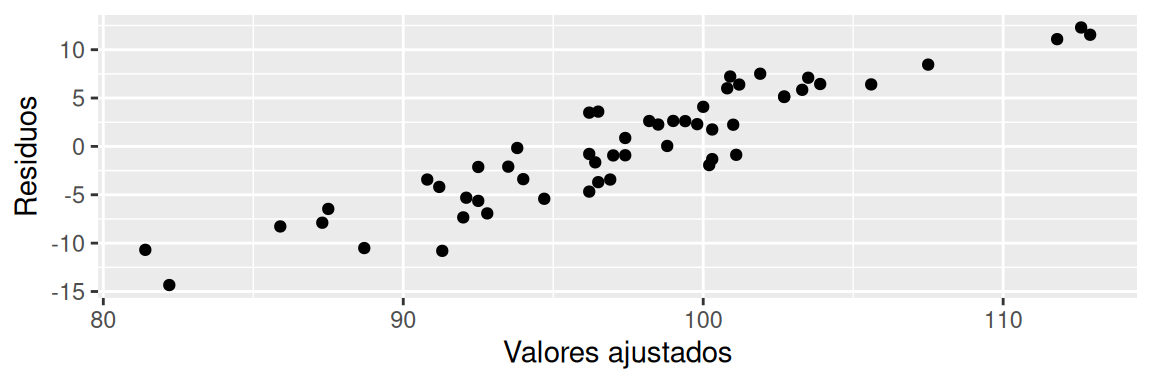
\includegraphics[width=\linewidth]{est2+inferencia_files/figure-latex/unnamed-chunk-120-1} \end{center}

Existe un claro patrón lineal, por lo cual, no se estaría cumpliendo con el supuesto de linealidad.

\begin{enumerate}
\def\labelenumi{\arabic{enumi}.}
\setcounter{enumi}{1}
\tightlist
\item
  \textbf{Normalidad}
\end{enumerate}

\begin{equation}
\notag
\begin{split}
H_0&: \text{Los residuos estandarizados tienen distribución Normal}\\
H_1&: \text{Los residuos estandarizados NO tienen distribución Normal}\\
\end{split}
\end{equation}

\begin{Shaded}
\begin{Highlighting}[]
\NormalTok{r\_e }\OtherTok{=} \FunctionTok{rstandard}\NormalTok{(modelo) }\CommentTok{\# residuos estandarizados}
\FunctionTok{shapiro.test}\NormalTok{(}\AttributeTok{x =}\NormalTok{ r\_e)}
\end{Highlighting}
\end{Shaded}

\begin{verbatim}
## 
##  Shapiro-Wilk normality test
## 
## data:  r_e
## W = 0.98827, p-value = 0.8738
\end{verbatim}

El valor-p de 0.8738 no es menor o igual a la significancia de 0.05, por lo cual, no existe suficiente evidencia estadística para rechaza la hipótesis nula, es decir, se asume que los residuos tienen distribución normal.Considerando una confianza del 95\%.

\begin{enumerate}
\def\labelenumi{\arabic{enumi}.}
\setcounter{enumi}{2}
\tightlist
\item
  \textbf{Homocedasticidad}
\end{enumerate}

\begin{equation}
\notag
\begin{split}
H_0&: \text{Los residuos tienen varianza constante}\\
H_1&: \text{Los residuos NO tienen varianza constante}\\
\end{split}
\end{equation}

\begin{Shaded}
\begin{Highlighting}[]
\NormalTok{df}\SpecialCharTok{$}\NormalTok{Valores.ajustados }\OtherTok{=}\NormalTok{ modelo}\SpecialCharTok{$}\NormalTok{fitted.values}
\FunctionTok{ggplot}\NormalTok{(}\AttributeTok{data =}\NormalTok{ df, }\FunctionTok{aes}\NormalTok{(}\AttributeTok{x =}\NormalTok{ Valores.ajustados, }\AttributeTok{y =}\NormalTok{ r\_e)) }\SpecialCharTok{+}
  \FunctionTok{geom\_point}\NormalTok{() }\SpecialCharTok{+} \FunctionTok{geom\_hline}\NormalTok{(}\AttributeTok{yintercept =} \DecValTok{0}\NormalTok{) }\SpecialCharTok{+}
  \FunctionTok{labs}\NormalTok{(}\AttributeTok{x =} \StringTok{"Valores ajustados"}\NormalTok{, }\AttributeTok{y =} \StringTok{"Residuos estandarizados"}\NormalTok{)}
\end{Highlighting}
\end{Shaded}

\begin{center}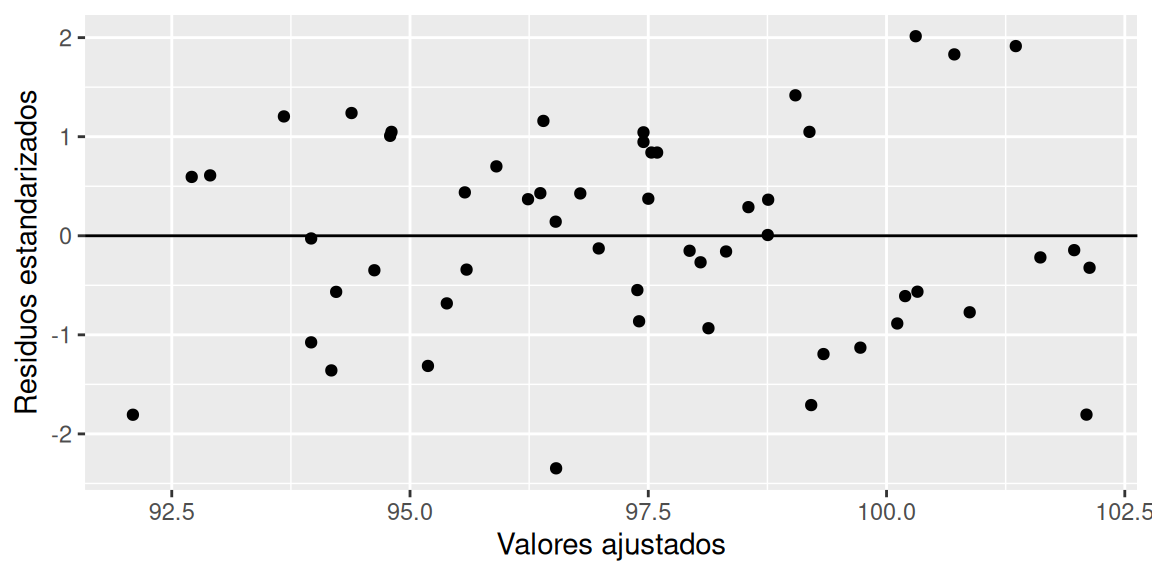
\includegraphics[width=\linewidth]{est2+inferencia_files/figure-latex/unnamed-chunk-122-1} \end{center}

No se evidencia patrones en la amplitud de los residuos, por lo que se asume homocedasticidad. Verificamos mediante la prueba de hipótesis correspondiente

\begin{Shaded}
\begin{Highlighting}[]
\FunctionTok{bptest}\NormalTok{(}\AttributeTok{formula =}\NormalTok{ Mineria }\SpecialCharTok{\textasciitilde{}}\NormalTok{ Ano }\SpecialCharTok{+}\NormalTok{ Industria, }\AttributeTok{data =}\NormalTok{ df)}
\end{Highlighting}
\end{Shaded}

\begin{verbatim}
## 
##  studentized Breusch-Pagan test
## 
## data:  Mineria ~ Ano + Industria
## BP = 1.4598, df = 2, p-value = 0.482
\end{verbatim}

El valor-p de 0.482 no es menor o igual a la significancia de 0.05, por lo cual, no existe suficiente evidencia estadística para rechazar la hipótesis nula, es decir, se asume que los residuos tiene varianza constante. Considerando una confianza del 95\%.

\begin{enumerate}
\def\labelenumi{\arabic{enumi}.}
\setcounter{enumi}{3}
\tightlist
\item
  \textbf{Independencia}
\end{enumerate}

\begin{equation}
\notag
\begin{split}
H_0&: \text{Autocorrelación de los residuos es igual a 0}\\
H_1&: \text{Autocorrelación de los residuos es distinta de 0}\\
\end{split}
\end{equation}

\begin{Shaded}
\begin{Highlighting}[]
\FunctionTok{dwtest}\NormalTok{(}\AttributeTok{formula =}\NormalTok{ Mineria }\SpecialCharTok{\textasciitilde{}}\NormalTok{ Ano }\SpecialCharTok{+}\NormalTok{ Industria, }\AttributeTok{data =}\NormalTok{ df, }\AttributeTok{alternative =} \StringTok{"two.sided"}\NormalTok{)}
\end{Highlighting}
\end{Shaded}

\begin{verbatim}
## 
##  Durbin-Watson test
## 
## data:  Mineria ~ Ano + Industria
## DW = 1.1949, p-value = 0.0009229
## alternative hypothesis: true autocorrelation is not 0
\end{verbatim}

El valor-p de 0.0009 es menor o igual a la significancia de 0.05, por lo cual, existe suficiente evidencia estadística para rechazar la hipótesis nula, es decir, se asume que los residuos no son independientes. Considerando una confianza del 95\%.
\end{example}

\begin{exercise}
Considere los modelos ajustados en:

\begin{itemize}
\tightlist
\item
  El ejercicio \ref{exr:co2}.
\item
  El ejercicio \ref{exr:calidad-aire}.
\end{itemize}

Estudie los supuestos del modelo, además escriba las hipótesis asociadas a los supuestos cuando corresponda, utilizando una confianza del 95\%.
\end{exercise}

\section{Selección de variables}\label{regresion-lineal-seleccion-variables}

La selección de métodos le permite especificar cómo se introducen las variables independientes en el análisis. Usando diferentes métodos, puede construir una variedad de modelos de regresión a partir del mismo conjunto de variables.

Dentro de las utilidades de usar un método para la selección de variables están:

\begin{itemize}
\tightlist
\item
  Evitar la colinealidad entre las covaribles.
\item
  Generar modelos parsimoniosos.
\end{itemize}

A continuación se dan a conocer algunos de los métodos de selección de variables.

\subsection{Forward}\label{regresion-lineal-seleccion-variables-forward}

Corresponde a un procedimiento de selección de variables paso a paso en el que las variables se ingresan secuencialmente en el modelo. La primera variable considerada para entrar en la ecuación de regresión es la que tiene la mayor correlación positiva o negativa con la variable dependiente. Esta variable se ingresa en la ecuación solo si cumple el criterio de entrada. Si se ingresa la primera variable, la variable independiente que no está en la ecuación y que tiene la mayor correlación parcial se considera a continuación. El procedimiento se detiene cuando no hay variables que cumplan con el criterio de entrada.

Los pasos detallados son los siguientes:

\begin{enumerate}
\def\labelenumi{\arabic{enumi}.}
\tightlist
\item
  Sea \(X_1\) la primera variable en ingresar al modelo, la que corresponde al predictor con mayor coeficiente de correlación lineal en valor absoluto con la variable respuesta.
\item
  Ajustar el modelo \(Y \sim X_1\). Si el modelo es significativo, continuar la selección. En caso contrario, reportar el modelo \(Y = \beta_0\).
\item
  Ajustar el modelo \(Y \sim X_1 + X_j\) para todo \(j = 2, \ldots , (p -1)\). Ingresar al modelo la variable con el mayor estadístico \(F\) parcial dado \(X_1\) (el menor valor-p) que sea significativo. Si no existen predictores significativos, reportar el modelo \(Y \sim X_1\).
\item
  Proseguir hasta que:

  \begin{itemize}
  \tightlist
  \item
    Se llegue a un número predeterminado de predictores en el modelo, o
  \item
    No se obtengan estadísticos \(F\) significativos.
  \end{itemize}
\end{enumerate}

El estadístico \(F\) mencionado en la metodología \emph{forward} prueba la siguiente hipótesis:

\begin{equation}
\begin{split}
H_0 &: \text{ La correlación parcial entre } X_j \text{ e } Y, \text{ dados } X_1, \ldots , X_{j-1}, \text{ es igual a cero}\\
H_1 &: \text{ La correlación parcial entre } X_j \text{ e } Y, \text{ dados } X_1, \ldots , X_{j-1}, \text{ es distinta cero}
\end{split}
\label{eq:forward}
\end{equation}

Más detalles del funcionamiento de este estadístico en el anexo \ref{F-forward}.

\begin{example}
\protect\hypertarget{exm:forward1}{}\label{exm:forward1}Considerando el ejercicio \ref{exr:ingreso}, elabore un modelo para estudiar la proporción de logro obtenida en el diagnóstico de lenguaje, seleccionado las variables independientes mediante el método \emph{forward}.

\begin{Shaded}
\begin{Highlighting}[]
\CommentTok{\# Cargamos la base de datos previamente, guardándola con el nombre "datos"}

\CommentTok{\# Planteamos un modelo vacío sin covariables, solo intercepto}
\NormalTok{modelo.nulo }\OtherTok{=} \FunctionTok{lm}\NormalTok{(Logro }\SpecialCharTok{\textasciitilde{}} \DecValTok{1}\NormalTok{, }\AttributeTok{data =}\NormalTok{ datos)}
\CommentTok{\# Planteamos un modelo con todas las covariables}
\NormalTok{modelo.total }\OtherTok{=} \FunctionTok{lm}\NormalTok{(Logro }\SpecialCharTok{\textasciitilde{}}\NormalTok{ ., }\AttributeTok{data =}\NormalTok{ datos)}
\NormalTok{modelo.final }\OtherTok{=} \FunctionTok{step}\NormalTok{(modelo.nulo, }\CommentTok{\# Modelo nulo}
                    \AttributeTok{scope =} \FunctionTok{list}\NormalTok{(}\AttributeTok{lower =} \FunctionTok{formula}\NormalTok{(modelo.nulo), }\CommentTok{\# Rango inicial de modelos examinados}
                                 \AttributeTok{upper =} \FunctionTok{formula}\NormalTok{(modelo.total)), }\CommentTok{\# Rango final de modelos examinados}
                    \AttributeTok{direction =} \StringTok{"forward"}\NormalTok{, }\CommentTok{\# Método de selección de variables}
                    \AttributeTok{trace =} \DecValTok{0}\NormalTok{, }\CommentTok{\# Si es igual a 0, no imprime todos los modelos que va elaborando, solo imprime el modelo final}
                    \AttributeTok{test =} \StringTok{"F"}\NormalTok{) }\CommentTok{\# Estadístico utilizado}
\FunctionTok{summary}\NormalTok{(modelo.final)}
\end{Highlighting}
\end{Shaded}

\begin{verbatim}
## 
## Call:
## lm(formula = Logro ~ LEN + NEM + Sexo, data = datos)
## 
## Residuals:
##      Min       1Q   Median       3Q      Max 
## -0.31796 -0.07033  0.00162  0.07968  0.26073 
## 
## Coefficients:
##               Estimate Std. Error t value Pr(>|t|)    
## (Intercept) -2.960e-01  7.173e-02  -4.126 5.44e-05 ***
## LEN          9.961e-04  1.013e-04   9.833  < 2e-16 ***
## NEM          3.372e-04  8.732e-05   3.861 0.000153 ***
## SexoMujer    2.665e-02  1.644e-02   1.621 0.106621    
## ---
## Signif. codes:  0 '***' 0.001 '**' 0.01 '*' 0.05 '.' 0.1 ' ' 1
## 
## Residual standard error: 0.1129 on 196 degrees of freedom
## Multiple R-squared:  0.3775, Adjusted R-squared:  0.3679 
## F-statistic: 39.61 on 3 and 196 DF,  p-value: < 2.2e-16
\end{verbatim}

¿Qué es posible comentar respecto a la inclusión de la variable Sexo en el modelo?
\end{example}

\begin{exercise}
\protect\hypertarget{exr:forward2}{}\label{exr:forward2}

Considerando el ejercicio \ref{exr:co2}, elabore un modelo para estudiar la tasa de absorción de dióxido de carbono de las plantas, seleccionado las variables independientes mediante el método \emph{forward}. Interprete los betas estimados, analice las pruebas de hipótesis asociadas a los betas e interprete el \(R^2\) ajustado del modelo. Se recomienda aplicar el siguiente código de manera previa:

\begin{Shaded}
\begin{Highlighting}[]
\NormalTok{data }\OtherTok{=}\NormalTok{ CO2}
\NormalTok{data}\SpecialCharTok{$}\NormalTok{Plant }\OtherTok{=} \FunctionTok{factor}\NormalTok{(data}\SpecialCharTok{$}\NormalTok{Plant, }\AttributeTok{ordered =}\NormalTok{ F)}
\end{Highlighting}
\end{Shaded}

\end{exercise}

\begin{exercise}
\protect\hypertarget{exr:forward3}{}\label{exr:forward3}Considerando el ejercicio \ref{exr:calidad-aire}, elabore un modelo para estudiar la concentración de Ozono en el aire, seleccionado las variables independientes mediante el método \emph{forward}. Interprete los betas estimados, analice las pruebas de hipótesis asociadas a los betas e interprete el \(R^2\) ajustado del modelo.
\end{exercise}

\subsection{Backward}\label{regresion-lineal-seleccion-variables-backward}

Al contrario de la metodología \emph{forward}, la metodología \emph{backward} realiza una eliminación de variables considerando como punto de partida el modelo que contiene todas las covariables. Los pasos detallados son los siguientes:

\begin{enumerate}
\def\labelenumi{\arabic{enumi}.}
\tightlist
\item
  Ajustar el modelo completo \((p − 1)\) veces, de modo de obtener los \((p − 1)\) estadísticos \(F\) parciales, dado que todas las variables restantes ya están en el modelo.
\item
  Eliminar el predictor con el menor estadístico \(F\) parcial (mayor valor-p) que no sea significativo. En caso de ser todos significativos, reportar el modelo completo.
\item
  Ajustar el modelo con los \((p − 2)\) predictores restantes, de modo de obtener los estadísticos \(F\) parciales de cada uno de ellos. Eliminar el predictor con el menor estadístico \(F\) parcial (mayor valor-p) que no sea significativo. En caso de ser todos significativos, reportar el modelo con \((p − 2)\) predictores.
\item
  Proseguir hasta que:

  \begin{itemize}
  \tightlist
  \item
    Se llegue a un número predeterminado de predictores en el modelo, o
  \item
    Todos los estadísticos \(F\) parciales sean significativos.
  \end{itemize}
\end{enumerate}

El estadístico \(F\) es el mismo que el aplicado en la metodología \emph{forward}.

\begin{example}
\protect\hypertarget{exm:backward1}{}\label{exm:backward1}

Considerando el ejercicio \ref{exr:calidad-aire}, elabore un modelo para estudiar la concentración de Ozono, seleccionado las variables independientes mediante el método \emph{backward}.

\begin{Shaded}
\begin{Highlighting}[]
\NormalTok{datos }\OtherTok{=}\NormalTok{ airquality}
\NormalTok{datos }\OtherTok{=} \FunctionTok{na.omit}\NormalTok{(datos)}
\CommentTok{\# Planteamos un modelo vacío sin covariables, solo intercepto}
\NormalTok{modelo.nulo }\OtherTok{=} \FunctionTok{lm}\NormalTok{(Ozone }\SpecialCharTok{\textasciitilde{}} \DecValTok{1}\NormalTok{, }\AttributeTok{data =}\NormalTok{ datos)}
\CommentTok{\# Planteamos un modelo con todas las covariables}
\NormalTok{modelo.total }\OtherTok{=} \FunctionTok{lm}\NormalTok{(Ozone }\SpecialCharTok{\textasciitilde{}}\NormalTok{ ., }\AttributeTok{data =}\NormalTok{ datos)}
\NormalTok{modelo.final }\OtherTok{=} \FunctionTok{step}\NormalTok{(modelo.total, }\CommentTok{\# Modelo total}
                    \AttributeTok{scope =} \FunctionTok{list}\NormalTok{(}\AttributeTok{lower =} \FunctionTok{formula}\NormalTok{(modelo.nulo), }\CommentTok{\# Rango inicial de modelos examinados}
                                 \AttributeTok{upper =} \FunctionTok{formula}\NormalTok{(modelo.total)), }\CommentTok{\# Rango final de modelos examinados}
                    \AttributeTok{direction =} \StringTok{"backward"}\NormalTok{, }\CommentTok{\# Método de selección de variables}
                    \AttributeTok{trace =} \DecValTok{0}\NormalTok{, }\CommentTok{\# Si es igual a 0, no imprime todos los modelos que va elaborando, solo imprime el modelo final}
                    \AttributeTok{test =} \StringTok{"F"}\NormalTok{) }\CommentTok{\# Estadístico utilizado}
\FunctionTok{summary}\NormalTok{(modelo.final)}
\end{Highlighting}
\end{Shaded}

\begin{verbatim}
## 
## Call:
## lm(formula = Ozone ~ Solar.R + Wind + Temp + Month, data = datos)
## 
## Residuals:
##     Min      1Q  Median      3Q     Max 
## -35.870 -13.968  -2.671   9.553  97.918 
## 
## Coefficients:
##              Estimate Std. Error t value Pr(>|t|)    
## (Intercept) -58.05384   22.97114  -2.527   0.0130 *  
## Solar.R       0.04960    0.02346   2.114   0.0368 *  
## Wind         -3.31651    0.64579  -5.136 1.29e-06 ***
## Temp          1.87087    0.27363   6.837 5.34e-10 ***
## Month        -2.99163    1.51592  -1.973   0.0510 .  
## ---
## Signif. codes:  0 '***' 0.001 '**' 0.01 '*' 0.05 '.' 0.1 ' ' 1
## 
## Residual standard error: 20.9 on 106 degrees of freedom
## Multiple R-squared:  0.6199, Adjusted R-squared:  0.6055 
## F-statistic: 43.21 on 4 and 106 DF,  p-value: < 2.2e-16
\end{verbatim}

\end{example}

\begin{exercise}
\protect\hypertarget{exr:contaminacion}{}\label{exr:contaminacion}En un estudio para explicar la tasa máxima de flujo de seis sectores de drenaje después de una tormenta, se desea analizar la relación entre el logaritmo de esta tasa (logq) y los siguientes predictores (\href{https://raw.githubusercontent.com/Dfranzani/Bases-de-datos-para-cursos/main/2023-1/drenaje.txt}{\emph{contaminacion.txt}}), a través de un modelo de regresión lineal múltiple:

\begin{itemize}
\tightlist
\item
  area: área del sector de drenaje.
\item
  area2: área impermeabilizada.
\item
  pendiente: pendiente media del sector.
\item
  largo: largo del flujo.
\item
  absorbencia: índice de absorbencia de la superficie (0: absorbencia total, 100: no absorbencia).
\item
  capacidad: capacidad estimada de almacenamiento del suelo.
\item
  infiltracion: tasa de infiltración del agua en el suelo.
\item
  lluvia: pulgadas de lluvia caída.
\item
  tiempo: tiempo en el cual la lluvia excedió 1/4 pulgadas/hora.
\end{itemize}

Determine dos modelos utilizando las metodologías forward y backward. Compare ambos modelos mediante el \(R^2\) ajustado. ¿Cuál modelo eligiría para estudiar la varible \emph{logq}?
\end{exercise}

\section{Predicción de observaciones}\label{regresion-lineal-prediccion-observaciones}

Es natural estar interesado en estudiar nuevas observaciones en un estudio, por ejemplo, si se construye una regresión lineal simple para estudiar el valor de dólar a través del PIB y el ICC, es posible que surja la pregunta ¿cuál será el valor del dólar para una PIB e ICC determinado? (considere que dichos valores del PIB e ICC no se encuentran en la muestra). Para responder a esto, es posible construir un denominado intervalo de predicción. Sin embargo, existe otro tipo de intervalo muy común, denominado intervalo de confianza. La distinción entre estos dos tipos de intervalos es la siguiente \citep[página 125]{fahrmeir_regression_2013}:

\begin{itemize}
\item
  Un intervalo de predicción es un intervalo asociado con una variable aleatoria aún por observar, con una probabilidad específica de que la variable aleatoria se encuentre dentro del intervalo.
\item
  Un intervalo de confianza es un intervalo asociado a un parámetro. Se supone que el parámetro no es aleatorio sino desconocido, y el intervalo de confianza se calcula a partir de los datos, con una probabilidad específica de que el intervalo contenga al parámetro.
\end{itemize}

Consideremos la base de datos \emph{airquality} del ejercicio \ref{exr:calidad-aire}. Para visualizar la diferencia entre los dos tipos de intervalos ajustemos una regresión lineal simple para estudiar la tasa de absorción del dióxido de carbono a través de la temperatura.

\begin{Shaded}
\begin{Highlighting}[]
\NormalTok{datos }\OtherTok{=}\NormalTok{ airquality}
\NormalTok{datos }\OtherTok{=} \FunctionTok{na.omit}\NormalTok{(datos)}
\NormalTok{modelo }\OtherTok{=} \FunctionTok{lm}\NormalTok{(Ozone }\SpecialCharTok{\textasciitilde{}}\NormalTok{ Temp, }\AttributeTok{data =}\NormalTok{ datos) }\CommentTok{\# Modelo}
\end{Highlighting}
\end{Shaded}

Al momento de obtener la información de los intervalos de confianza y predicción se incluye el valor central del intervalo (el mismo para ambos), además del valor inferior y superior de cada uno.

\begin{Shaded}
\begin{Highlighting}[]
\NormalTok{I\_confianza }\OtherTok{=} \FunctionTok{predict.lm}\NormalTok{(modelo, }\AttributeTok{interval =} \StringTok{"confidence"}\NormalTok{) }\CommentTok{\# Intervalos de confianza}
\NormalTok{I\_prediccion }\OtherTok{=} \FunctionTok{predict.lm}\NormalTok{(modelo, }\AttributeTok{interval =} \StringTok{"prediction"}\NormalTok{) }\CommentTok{\# Intervalos de predicción}
\FunctionTok{head}\NormalTok{(I\_confianza,}\DecValTok{3}\NormalTok{)}
\end{Highlighting}
\end{Shaded}

\begin{verbatim}
##        fit       lwr      upr
## 1 15.77429  8.958438 22.59014
## 2 27.96984 22.697411 33.24227
## 3 32.84806 28.001893 37.69423
\end{verbatim}

\begin{Shaded}
\begin{Highlighting}[]
\FunctionTok{head}\NormalTok{(I\_prediccion,}\DecValTok{3}\NormalTok{)}
\end{Highlighting}
\end{Shaded}

\begin{verbatim}
##        fit       lwr      upr
## 1 15.77429 -32.12231 63.67089
## 2 27.96984 -19.73159 75.67127
## 3 32.84806 -14.80814 80.50426
\end{verbatim}

El gráfico \ref{fig:IC-IP} refleja los dos tipos de intervalo.

\begin{Shaded}
\begin{Highlighting}[]
\NormalTok{df\_grafico }\OtherTok{=} \FunctionTok{data.frame}\NormalTok{(}\StringTok{"y"} \OtherTok{=}\NormalTok{ datos}\SpecialCharTok{$}\NormalTok{Ozone, }
                        \StringTok{"x"} \OtherTok{=}\NormalTok{ datos}\SpecialCharTok{$}\NormalTok{Temp,}
                        \StringTok{"Confianza\_lower"} \OtherTok{=}\NormalTok{ I\_confianza[,}\DecValTok{2}\NormalTok{],}
                        \StringTok{"Confianza\_upper"} \OtherTok{=}\NormalTok{ I\_confianza[,}\DecValTok{3}\NormalTok{],}
                        \StringTok{"Prediccion\_lower"} \OtherTok{=}\NormalTok{ I\_prediccion[,}\DecValTok{2}\NormalTok{],}
                        \StringTok{"Prediccion\_upper"} \OtherTok{=}\NormalTok{ I\_prediccion[,}\DecValTok{3}\NormalTok{])}
\FunctionTok{library}\NormalTok{(ggplot2)}
\FunctionTok{ggplot}\NormalTok{(}\AttributeTok{data =}\NormalTok{ df\_grafico, }\FunctionTok{aes}\NormalTok{(}\AttributeTok{x =}\NormalTok{ x, }\AttributeTok{y =}\NormalTok{ y)) }\SpecialCharTok{+} \FunctionTok{geom\_point}\NormalTok{() }\SpecialCharTok{+}
  \FunctionTok{geom\_smooth}\NormalTok{(}\AttributeTok{method =} \StringTok{"lm"}\NormalTok{, }\AttributeTok{formula =}\NormalTok{ y }\SpecialCharTok{\textasciitilde{}}\NormalTok{ x, }\AttributeTok{se =} \ConstantTok{FALSE}\NormalTok{, }\AttributeTok{linewidth =} \FloatTok{0.5}\NormalTok{) }\SpecialCharTok{+}
  \FunctionTok{geom\_line}\NormalTok{(}\FunctionTok{aes}\NormalTok{(}\AttributeTok{x =}\NormalTok{ x, }\AttributeTok{y =}\NormalTok{ Confianza\_lower, }\AttributeTok{color =} \StringTok{"IC"}\NormalTok{), }\AttributeTok{linetype =} \DecValTok{2}\NormalTok{) }\SpecialCharTok{+}
  \FunctionTok{geom\_line}\NormalTok{(}\FunctionTok{aes}\NormalTok{(}\AttributeTok{x =}\NormalTok{ x, }\AttributeTok{y =}\NormalTok{ Confianza\_upper, }\AttributeTok{color =} \StringTok{"IC"}\NormalTok{), }\AttributeTok{linetype =} \DecValTok{2}\NormalTok{) }\SpecialCharTok{+}
  \FunctionTok{geom\_line}\NormalTok{(}\FunctionTok{aes}\NormalTok{(}\AttributeTok{x =}\NormalTok{ x, }\AttributeTok{y =}\NormalTok{ Prediccion\_lower, }\AttributeTok{color =} \StringTok{"IP"}\NormalTok{), }\AttributeTok{linetype =} \DecValTok{2}\NormalTok{) }\SpecialCharTok{+}
  \FunctionTok{geom\_line}\NormalTok{(}\FunctionTok{aes}\NormalTok{(}\AttributeTok{x =}\NormalTok{ x, }\AttributeTok{y =}\NormalTok{ Prediccion\_upper, }\AttributeTok{color =} \StringTok{"IP"}\NormalTok{), }\AttributeTok{linetype =} \DecValTok{2}\NormalTok{) }\SpecialCharTok{+}
  \FunctionTok{labs}\NormalTok{(}\AttributeTok{x =} \StringTok{"Temperatura"}\NormalTok{ , }\AttributeTok{y =} \StringTok{"Ozono"}\NormalTok{, }\AttributeTok{color =} \StringTok{"Intervalos"}\NormalTok{,}
       \AttributeTok{title =} \StringTok{"Intervalo de confianza (IC) y predicción (IP)"}\NormalTok{)}
\end{Highlighting}
\end{Shaded}

\begin{figure}

{\centering 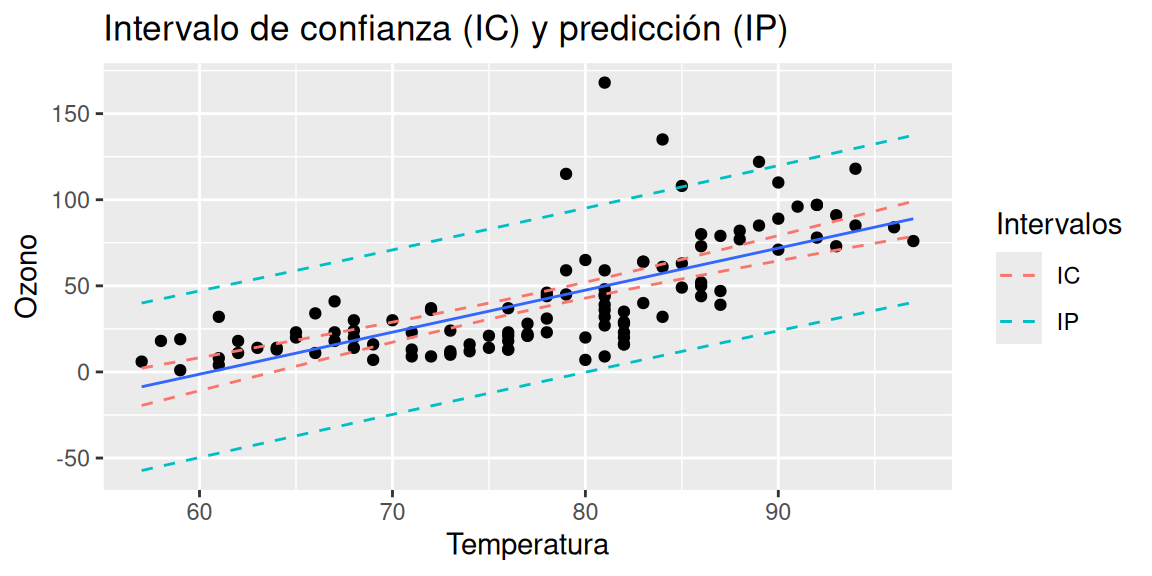
\includegraphics[width=\linewidth]{est2+inferencia_files/figure-latex/IC-IP-1} 

}

\caption{Intervalo de confianza y predicción}\label{fig:IC-IP}
\end{figure}

Ahora, para responder a preguntas como ¿cuál sería la concentración de ozono a una temperatura de 90.34 grados Fahrenheit? se debe reportar el intervalo de predicción, el cual, en R, es al 95\% de confianza por defecto.

\begin{Shaded}
\begin{Highlighting}[]
\CommentTok{\# Creamos una nueva base de datos para poder consultar el intervalo de predicción}
\CommentTok{\# Se debe tener el cuidado de que las columnas tengan el mismo nombre que base usada}
\CommentTok{\# para construir el modelo de regresión lineal}
\NormalTok{aux }\OtherTok{=} \FunctionTok{data.frame}\NormalTok{(}\StringTok{"Temp"} \OtherTok{=} \FloatTok{90.34}\NormalTok{) }\CommentTok{\# Solo incluimos la(s) variable(s) independiente(s)}
\FunctionTok{predict.lm}\NormalTok{(modelo, }\AttributeTok{newdata =}\NormalTok{ aux, }\AttributeTok{interval =} \StringTok{"prediction"}\NormalTok{)}
\end{Highlighting}
\end{Shaded}

\begin{verbatim}
##        fit      lwr      upr
## 1 72.70312 24.71044 120.6958
\end{verbatim}

La salida de R indica, que la predicción de la concentración de ozono asociado a una medición de temperatura de 90.34 grados Fahrenheit sería de 72.70312 partes por billón, mientras que, el intervalo de predicción al 95\% de confianza es \((24.71044, 120.6958)\).

Por otro lado, si se desea conocer el intervalo de confianza asociado a un valor promedio (esperado o ajustado) del ozono asociado a una temperatura de 90.34 grados Fahrenheit, se debe efectuar el siguiente comando.

\begin{Shaded}
\begin{Highlighting}[]
\FunctionTok{predict.lm}\NormalTok{(modelo, }\AttributeTok{newdata =}\NormalTok{ aux, }\AttributeTok{interval =} \StringTok{"confidence"}\NormalTok{)}
\end{Highlighting}
\end{Shaded}

\begin{verbatim}
##        fit      lwr      upr
## 1 72.70312 65.24199 80.16425
\end{verbatim}

La salida de R indica, que el valor promedio de la concentración de ozono asociado a una medición de temperatura de 90.34 grados Fahrenheit sería de 72.70312 partes por billón, mientras que, el intervalo de confianza al 95\% de confianza es \((65.24199, 80.16425)\).

\begin{exercise}

Utilizando la base del ejercicio \ref{exr:contaminacion} realice lo siguiente:

\begin{enumerate}
\def\labelenumi{\arabic{enumi}.}
\tightlist
\item
  Ajuste en R un modelo de regresión lineal para estudiar el logaritmo de la tasa máxima de flujo de seis sectores de drenaje después de una tormenta (logq) a través de las pulgadas de lluvia caída.
\item
  Escriba la ecuación de regresión ajustada.
\item
  Interprete los betas estimados.
\item
  Elabore un gráfico de dispersión entre la variable dependiente e independiente del modelo de regresión lineal, que contenga los intervalos de confianza y predicción, diferenciándolos por colores.
\item
  Determine el intervalo de predicción de logaritmo de la tasa máxima de flujo de seis sectores de drenaje después de una tormenta (logq) asociado a una cantidad de lluvia caída de 3.435 pulgadas. Interprete.
\item
  Determine el intervalo de confianza del valor promedio del logaritmo de la tasa máxima de flujo de seis sectores de drenaje después de una tormenta (logq) asociado a una cantidad de lluvia caída de 3.435 pulgadas. Interprete.
\end{enumerate}

\end{exercise}

\begin{exercise}

Las mujeres ocupan aproximadamente la mitad de la población mundial, pero cuando se trata de la fuerza laboral total de un país, el porcentaje de trabajadores masculinos y femeninos rara vez es similar. Esto es aún más prominente para los países en desarrollo y subdesarrollados. Si bien varias razones, como el acceso insuficiente a la educación, las supersticiones religiosas y la falta de infraestructuras adecuadas, son responsables de esta discrepancia, va mucho más allá. Y para mostrar los efectos de múltiples factores socioeconómicos sobre la participación de la mujer en la fuerza laboral total, se ha considerado el porcentaje de empleo femenino en la fuerza laboral total, entre otros.

El conjunto de datos (\href{https://raw.githubusercontent.com/Dfranzani/Bases-de-datos-para-cursos/main/2023-1/Empleo\%2Bfemenino.csv}{Empleo+femenino.csv}) se eligió de una encuesta realizada en la población de Bangladesh. La base de datos contiene los siguientes datos:

\begin{itemize}
\tightlist
\item
  Year: Año de medición.
\item
  PerFemEmploy: Relación entre empleo y población (\%) de mujeres de 15 años o más.
\item
  Ratio\_MaletoFemale: Relación entre la tasa de participación de mujeres y hombres en la fuerza laboral. La tasa de participación en la fuerza laboral es la proporción de la población de 15 años o más que es económicamente activa.
\item
  Wage.Salaried: Trabajadores asalariados, mujeres (\% del empleo femenino). Los trabajadores asalariados (empleados) son aquellos trabajadores que ocupan el tipo de trabajos definidos como ``trabajos de empleo remunerado''.
\end{itemize}

A continuación:

\begin{enumerate}
\def\labelenumi{\arabic{enumi}.}
\tightlist
\item
  Ajuste en R un modelo mediante la metodología forward para estudiar la variable \emph{PerFemEmploy.}
\item
  Escriba el modelo poblacional.
\item
  Escriba el modelo ajustado.
\item
  Escriba la ecuación de regresión ajustada.
\item
  Interprete los parámetros estimados.
\item
  Estudie las pruebas de hipótesis de no nulidad (individual y conjunta) utilizando una confianza del 95\%.
\item
  Determine el intervalo de predicción de la variable \emph{PerFemEmploy} asociada a una tasa de participación de mujeres y hombres en la fuerza laboral igual a 37.543 en el año 2020. Interprete.
\item
  Determine el intervalo de confianza del valor promedio de la variable \emph{PerFemEmploy} asociada a una tasa de participación de mujeres y hombres en la fuerza laboral igual a 45.121 en el año 2021. Interprete.
\item
  Interprete el \(R^2\) ajustado.
\item
  Estudie los supuestos del modelo, utilizando una confianza del 95\%.
\end{enumerate}

\end{exercise}

\section{Ejercicios}\label{ejercicios-unidad-3}

A continuación, desarrolle los ejercicios manualmente sin el uso de R.

\begin{exercise}
En un estudio de marketing se observa el gasto en publicidad digital \(X\) (miles de \$) y las ventas semanales \(Y\) (miles de unidades) para pequeños comercios durante cinco semanas consecutivas; los pares están emparejados por orden: \(X\): 2.0, 2.5, 3.0, 3.5, 4.0; \(Y\): 15, 16, 18, 19, 21. Calcule manualmente los estimadores de la recta de regresión lineal simple \(Y=\beta_0+\beta_1 X+\varepsilon\).
\end{exercise}

\begin{exercise}
Una empresa logística registra la cantidad de repartidores en turno \(X\) y el número de entregas completadas \(Y\) por día en siete jornadas; los datos están emparejados por orden: \(X\): 5, 6, 7, 8, 9, 10, 11; \(Y\): 42, 45, 47, 50, 52, 55, 58. Estime manualmente \(\hat\beta_1\) y \(\hat\beta_0\) de la regresión lineal simple \(Y=\beta_0+\beta_1 X+\varepsilon\).
\end{exercise}

\begin{exercise}
Para un e-commerce se registra el tiempo de carga promedio del sitio \(X\) (segundos) y la tasa de conversión \(Y\) (\%) en ocho días de test A/B; los pares \((X,Y)\) están en el mismo orden: \(X\): 1.8, 2.0, 2.2, 2.4, 2.6, 2.8, 3.0, 3.2; \(Y\): 3.9, 3.8, 3.7, 3.5, 3.4, 3.3, 3.1, 3.0. Calcule manualmente \(\hat\beta_1\) y \(\hat\beta_0\) de \(Y=\beta_0+\beta_1 X+\varepsilon\).
\end{exercise}

\begin{exercise}
Un analista de precios observa el descuento aplicado \(X\) (\%) y la cantidad vendida \(Y\) (unidades) para nueve promociones del último mes, emparejadas por orden: \(X\): 0, 2, 4, 6, 8, 10, 12, 14, 16; \(Y\): 120, 125, 130, 138, 142, 150, 155, 160, 168. Determine manualmente \(\hat\beta_1\) y \(\hat\beta_0\) de la regresión \(Y=\beta_0+\beta_1 X+\varepsilon\).
\end{exercise}

\begin{exercise}
Considere una variable aleatoria \(Y\) con observaciones \(y_1, y_2, \ldots, y_n\). Muestre que:
\[
\sum_{i=1}^n (y_i - \bar{y})^2 = \sum_{i=1}^n y_i^2 - n \bar{y}^2
\]
\end{exercise}

\begin{exercise}
Sea el modelo de regresión lineal simple \(Y_i = \beta_0 + \beta_1 X_i + \varepsilon_i\). A partir de los estimadores de mínimos cuadrados \(\hat\beta_0\) y \(\hat\beta_1\), demuestre la identidad de descomposición de la suma de cuadrados:
\[
\text{SCR} = \text{SCReg} + \text{SCE}
\]
\end{exercise}

\begin{exercise}
En el modelo de regresión lineal simple \(Y_i = \beta_0 + \beta_1 X_i + \varepsilon_i\), utilice los resultados de mínimos cuadrados para demostrar que
\[
\sum_{i=1}^n (y_i - \bar{y})(x_i - \bar{x}) = \hat\beta_1 \sum_{i=1}^n (x_i - \bar{x})^2
\]

Explique cómo esta igualdad garantiza que \(\hat\beta_1 = \frac{S_{xy}}{S_{xx}}\).
\end{exercise}

\begin{exercise}
Sean \(X\) y \(Y\) variables aleatorias de un muestra de tamaño \(n\). Considere el siguiente modelo de regresión lineal simple:

\[
Y_i = \beta_0 + \beta_1X_i + \varepsilon_i, \varepsilon_i \overset{iid}{\sim} N(0, \sigma^2)
\]

Demuestre que:

El estimador de mínimos cuadrados de \(\beta_1\) es \(\hat{\beta}_1 = \displaystyle\frac{\displaystyle\sum_{i=1}^n(X_i - \bar{X})(Y_i - \bar{Y})}{\displaystyle\sum_{i=1}^n(X_i - \bar{X})^2}\)
\end{exercise}

\begin{exercise}
Sean \(X\) y \(Y\) variables aleatorias de un muestra de tamaño \(n\). Considere el siguiente modelo de regresión lineal simple:

\[
Y_i = \beta_0 + \beta_1X_i + \varepsilon_i, \varepsilon_i \overset{iid}{\sim} N(0, \sigma^2)
\]

Demuestre que el estimador de mínimos cuadrados de \(\beta_0\) es \(\widehat{\beta}_0 = \bar{Y} - \beta_1\bar{X}\)
\end{exercise}

\begin{exercise}
Sean \(X\) y \(Y\) variables aleatorias de un muestra de tamaño \(n\). Considere el siguiente modelo de regresión lineal simple:

\[
Y_i = \beta_0 + \beta_1X_i + \varepsilon_i, \varepsilon_i \overset{iid}{\sim} N(0, \sigma^2)
\]

Demuestre que:

\[
\widehat{Y}_i = \bar{Y} + r_{XY}\displaystyle\frac{S_Y}{S_X}(X_i-\bar{X})
\]
\end{exercise}

\begin{exercise}
Sean \(X\) y \(Y\) variables aleatorias de un muestra de tamaño \(n\). Considere el siguiente modelo de regresión lineal simple:

\[
Y_i = \beta_0 + \beta_1X_i + \varepsilon_i, \varepsilon_i \overset{iid}{\sim} N(0, \sigma^2)
\]

Demuestre que:

\[
R^2 = r_{XY}^2
\]
\end{exercise}

\begin{exercise}
Se desea modelar el rendimiento de combustible (millas por galón, \(Y=\text{mpg}\)) en función del peso del automóvil (miles de libras, \(X=\text{wt}\)) usando la base \textbf{mtcars} de R (32 automóviles; variables relevadas por \emph{Motor Trend}, 1974). A continuación se muestra el ajuste de una regresión lineal simple \(Y=\beta_0+\beta_1 X+\varepsilon\) ejecutado en R (se asume normalidad de los residuos y homocedasticidad). Código:

\begin{Shaded}
\begin{Highlighting}[]
\FunctionTok{data}\NormalTok{(mtcars)}
\NormalTok{ajuste }\OtherTok{=} \FunctionTok{lm}\NormalTok{(mpg }\SpecialCharTok{\textasciitilde{}}\NormalTok{ wt, }\AttributeTok{data =}\NormalTok{ mtcars)}
\FunctionTok{summary}\NormalTok{(ajuste)}
\end{Highlighting}
\end{Shaded}

\begin{verbatim}
## 
## Call:
## lm(formula = mpg ~ wt, data = mtcars)
## 
## Residuals:
##     Min      1Q  Median      3Q     Max 
## -4.5432 -2.3647 -0.1252  1.4096  6.8727 
## 
## Coefficients:
##             Estimate Std. Error t value Pr(>|t|)    
## (Intercept)  37.2851     1.8776  19.858  < 2e-16 ***
## wt           -5.3445     0.5591  -9.559 1.29e-10 ***
## ---
## Signif. codes:  0 '***' 0.001 '**' 0.01 '*' 0.05 '.' 0.1 ' ' 1
## 
## Residual standard error: 3.046 on 30 degrees of freedom
## Multiple R-squared:  0.7528, Adjusted R-squared:  0.7446 
## F-statistic: 91.38 on 1 and 30 DF,  p-value: 1.294e-10
\end{verbatim}

Interprete los parámetros estimados y las pruebas de no nulidad con una confianza del 95\%. Además, escriba la ecuación de regresión poblacional y ajustada.
\end{exercise}

\begin{exercise}
Se estudia la relación entre el tiempo de espera en un restaurante (\(Y=\text{waiting}\), minutos) y la duración de la erupción de un géiser (\(X=\text{eruptions}\), minutos) usando la base \textbf{faithful} de R (272 observaciones recogidas en el géiser \emph{Old Faithful}, Yellowstone). A continuación se muestra el ajuste de una regresión lineal simple \(Y=\beta_0+\beta_1 X+\varepsilon\). Código:

\begin{Shaded}
\begin{Highlighting}[]
\FunctionTok{data}\NormalTok{(faithful)}
\NormalTok{ajuste }\OtherTok{=} \FunctionTok{lm}\NormalTok{(waiting }\SpecialCharTok{\textasciitilde{}}\NormalTok{ eruptions, }\AttributeTok{data =}\NormalTok{ faithful)}
\FunctionTok{summary}\NormalTok{(ajuste)}
\end{Highlighting}
\end{Shaded}

\begin{verbatim}
## 
## Call:
## lm(formula = waiting ~ eruptions, data = faithful)
## 
## Residuals:
##      Min       1Q   Median       3Q      Max 
## -12.0796  -4.4831   0.2122   3.9246  15.9719 
## 
## Coefficients:
##             Estimate Std. Error t value Pr(>|t|)    
## (Intercept)  33.4744     1.1549   28.98   <2e-16 ***
## eruptions    10.7296     0.3148   34.09   <2e-16 ***
## ---
## Signif. codes:  0 '***' 0.001 '**' 0.01 '*' 0.05 '.' 0.1 ' ' 1
## 
## Residual standard error: 5.914 on 270 degrees of freedom
## Multiple R-squared:  0.8115, Adjusted R-squared:  0.8108 
## F-statistic:  1162 on 1 and 270 DF,  p-value: < 2.2e-16
\end{verbatim}

Interprete los parámetros estimados y las pruebas de no nulidad con una confianza del 95\%. Además, escriba la ecuación de regresión poblacional y ajustada.
\end{exercise}

\begin{exercise}
\leavevmode

\item

Considere el siguiente modelo de regresión lineal simple:

\[
Y_i = \beta_0 + \beta_1X_i + \varepsilon, \varepsilon_i \overset{iid}{\sim} N(0, \sigma^2) \text{ ,} i = 1, \ldots, n = 74
\]

Utilizando los datos que se muestran a continuación, calcule lo siguiente: \(R^2\), Error estándar residual, \(F_0\) de la prueba de no nulidad conjunta y los EMC de \(\beta_0\) y \(\beta_1\). Trabaje con 4 decimales.

\begin{table}[H]
\centering
\resizebox{\ifdim\width>\linewidth\linewidth\else\width\fi}{!}{
\begin{tabular}[t]{llll}
\toprule
$\displaystyle\sum_{i=1}^n \widehat{y}_i = 6704.54$ & $\displaystyle\sum_{i=1}^n y_i\widehat{y}_i = 616140.32$ & $\displaystyle\sum_{i=1}^n y_ix_i = 665482.26$ & $\displaystyle\sum_{i=1}^n y_i = 6704.54$\\
$\displaystyle\sum_{i=1}^n \widehat{y}_i^2 = 616140.32$ & $\displaystyle\sum_{i=1}^n y_i^2 = 635642.36$ & $\displaystyle\sum_{i=1}^n x_i = 7421.21$ & $\displaystyle\sum_{i=1}^n x_i^2 = 749710.79$\\
\bottomrule
\end{tabular}}
\end{table}

\end{exercise}

\begin{exercise}

Considere el siguiente modelo de regresión lineal simple:
\[
Y_i=\beta_0+\beta_1 X_i+\varepsilon_i,\quad \varepsilon_i\overset{iid}{\sim}N(0,\sigma^2),\quad i=1,\ldots,n=60
\]
Utilizando las sumatorias que se muestran a continuación, calcule: \(R^2\), el error estándar residual, el estadístico \(F_0\) de la prueba de no nulidad conjunta y los EMC de \(\beta_0\) y \(\beta_1\). Trabaje con 4 decimales.

\begin{table}[H]
\centering
\resizebox{\ifdim\width>\linewidth\linewidth\else\width\fi}{!}{
\begin{tabular}[t]{llll}
\toprule
$\displaystyle\sum_{i=1}^n \widehat{y}_i = 780.00$ & $\displaystyle\sum_{i=1}^n y_i\,\widehat{y}_i = 11598.00$ & $\displaystyle\sum_{i=1}^n x_i y_i = 6435.00$ & $\displaystyle\sum_{i=1}^n y_i = 780.00$\\
$\displaystyle\sum_{i=1}^n \widehat{y}_i^2 = 11598.00$ & $\displaystyle\sum_{i=1}^n y_i^2 = 12500.00$ & $\displaystyle\sum_{i=1}^n x_i = 450.00$ & $\displaystyle\sum_{i=1}^n x_i^2 = 3700.00$\\
\bottomrule
\end{tabular}}
\end{table}

\end{exercise}

\begin{exercise}
Considere el modelo de regresión lineal múltiple con dos regresores:
\[
Y = \beta_0 + \beta_1 X_1 + \beta_2 X_2 + \varepsilon,
\]
donde \(\varepsilon \sim N(0,\sigma^2I_n)\).

Se entrega la siguiente \textbf{matriz de diseño} \(X\) (incluyendo la columna de unos para el intercepto) y el vector de respuestas \(Y\):

\[
X =
\begin{bmatrix}
1 & 2 & 3 \\
1 & 4 & 2 \\
1 & 5 & 6 \\
1 & 7 & 5
\end{bmatrix},
\quad
Y =
\begin{bmatrix}
10 \\
12 \\
20 \\
23
\end{bmatrix}.
\]

Calcule los \textbf{estimadores de mínimos cuadrados ordinarios} de los parámetros \(\beta_0, \beta_1, \beta_2\), mostrando explícitamente los cálculos de \(X^tX\), \(X^tY\), \((X^tX)^{-1}\) y finalmente el vector de estimadores \(\hat\beta\).
\end{exercise}

\begin{exercise}
Considere el modelo de regresión lineal múltiple con dos regresores
\[
Y=\beta_0+\beta_1X_1+\beta_2X_2+\varepsilon,\qquad \varepsilon\sim N(0,\sigma^2I_n).
\]
Se entrega la \textbf{matriz de diseño} \(X\) (incluye intercepto) y el \textbf{vector de respuestas} \(Y\), con valores \textbf{decimales} no redondeados:
\[
X=
\begin{bmatrix}
1 & 1.3 & 2.7\\
1 & 2.1 & 1.4\\
1 & 3.8 & 4.2\\
1 & 4.5 & 3.1\\
1 & 2.9 & 5.6\\
1 & 5.2 & 4.7
\end{bmatrix},\quad
Y=
\begin{bmatrix}
7.4\\
8.9\\
13.2\\
14.8\\
12.1\\
17.3
\end{bmatrix}.
\]

Calcule los estimadores MCO. Obtenga los valores ajustados \(\hat Y=X\hat\beta\). Calcule la matriz de residuos. Calcule las SCT, SCReg, SCR, el MCE y el error estándar residual.
\end{exercise}

\begin{exercise}

Utilice la siguiente tabla (que contiene un resumen de salidas en R) para estudiar los supuestos de Homocedasticidad, Independencia y Normalidad de un modelo de regresión lineal múltiple ajustado a una base de datos simulada de ingresos (\(Y\)) en función de edad (\(X_1\)) y nivel educacional (\texttt{educacion}) (\(X_2\)). Indique la fila del código seleccionado para cada supuesto, justificando su elección. Además, escriba las pruebas de hipótesis involucradas e interprete utilizando una confianza del 96\%.

\begin{table}[H]
\centering
\resizebox{\ifdim\width>\linewidth\linewidth\else\width\fi}{!}{
\begin{tabular}[t]{llll}
\toprule
 & Prueba de hipótesis & Valor-p & Datos utilizados en el comando de R\\
\midrule
1 & Breusch-Pagan & 0.0440 & edad $\sim$ ingresos\\
2 & Durbin-Watson & 0.0674 & ingresos $\sim$ edad + educacion\\
3 & Anderson-Darling & 0.0278 & modelo\$y\\
4 & Shapiro-Wilk & 0.0345 & modelo\$y\\
5 & Shapiro-Wilk & 0.0812 & residuos estandarizados\\
6 & Durbin-Watson & 0.0156 & ingresos $\sim$ educacion\\
7 & Breusch-Pagan & 0.0119 & ingresos $\sim$ region + edad + educacion\\
8 & Durbin-Watson & 0.0523 & edad \sim ingresos + educacion\\
9 & Breusch-Pagan & 0.0925 & ingresos $\sim$ edad + educacion\\
\bottomrule
\end{tabular}}
\end{table}

\end{exercise}

\begin{exercise}

Utilice la siguiente tabla (que contiene un resumen de salidas en R) para estudiar los supuestos de Homocedasticidad, Independencia y Normalidad de un modelo de regresión lineal múltiple ajustado a una base simulada donde \(Y=\) ventas y \(X_=\) precio. Indique la fila del código seleccionado para cada supuesto, justificando su elección. Además, escriba las pruebas de hipótesis involucradas e interprete utilizando una confianza del 95\%.

\begin{table}[H]
\centering
\resizebox{\ifdim\width>\linewidth\linewidth\else\width\fi}{!}{
\begin{tabular}[t]{llll}
\toprule
 & Prueba de hipótesis & Valor-p & Datos utilizados en el comando de R\\
\midrule
1 & Durbin-Watson & 0.0724 & ventas $\sim$ publicidad\\
2 & Shapiro-Wilk & 0.0198 & modelo\$residuals\\
3 & Shapiro-Wilk & 0.0613 & residuos estandarizados\\
4 & Durbin-Watson & 0.0589 & publicidad $\sim$ ventas\\
5 & Anderson-Darling & 0.0335 & modelo\$residuals\\
6 & Breusch-Pagan & 0.0221 & ventas $\sim$ precio\\
7 & Breusch-Pagan & 0.0870 & ventas $\sim$ publicidad\\
8 & Durbin-Watson & 0.0126 & ventas $\sim$ precio\\
9 & Breusch-Pagan & 0.0417 & ventas $\sim$ region\\
\bottomrule
\end{tabular}}
\end{table}

\end{exercise}

\begin{exercise}

Se desea ajustar un modelo de regresión lineal múltiple con variables cualitativas para explicar el rendimiento de combustible \(Y=\text{mpg}\) (millas por galón) en función del \textbf{peso} del automóvil \(X_1=\text{wt}\) (en miles de libras) y dos variables categóricas de la base \textbf{mtcars} de R: \textbf{transmisión} \(X_2=\text{am}\) (0=automática, 1=manual) y \textbf{cilindrada} \(X_3=\text{cyl}\) (niveles: 4, 6, 8 cilindros). Se asume codificación de tratamiento con categorías de referencia \textbf{am=0} (automática) y \textbf{cyl=4} (4 cilindros). A continuación se muestra el código y la salida de R para el ajuste \(\text{mpg} \sim \text{wt} + \text{factor(am)} + \text{factor(cyl)}\).

\begin{verbatim}
## 
## Call:
## lm(formula = mpg ~ wt + am + cyl, data = mt)
## 
## Residuals:
##     Min      1Q  Median      3Q     Max 
## -4.4898 -1.3116 -0.5039  1.4162  5.7758 
## 
## Coefficients:
##             Estimate Std. Error t value Pr(>|t|)    
## (Intercept)  33.7536     2.8135  11.997  2.5e-12 ***
## wt           -3.1496     0.9080  -3.469  0.00177 ** 
## ammanual      0.1501     1.3002   0.115  0.90895    
## cyl6         -4.2573     1.4112  -3.017  0.00551 ** 
## cyl8         -6.0791     1.6837  -3.611  0.00123 ** 
## ---
## Signif. codes:  0 '***' 0.001 '**' 0.01 '*' 0.05 '.' 0.1 ' ' 1
## 
## Residual standard error: 2.603 on 27 degrees of freedom
## Multiple R-squared:  0.8375, Adjusted R-squared:  0.8134 
## F-statistic: 34.79 on 4 and 27 DF,  p-value: 2.73e-10
\end{verbatim}

\begin{enumerate}
\def\labelenumi{\arabic{enumi}.}
\item
  Escriba la ecuación de regresión poblacional indicando la categoría de referencia.
\item
  Escriba la ecuación ajustada.
\item
  Interprete los parámetros estimados en su contexto y con la codificación usada, indicando unidades y sentido del efecto.
\item
  Evalúe las pruebas de no nulidad de cada coeficiente usando la salida (valores t y p-values). Indique, con un nivel de confianza del 95\%, qué efectos son estadísticamente significativos.
\item
  Comente las métricas del modelo: Error estándar residual y R\^{}2 ajustado.
\end{enumerate}

\end{exercise}

\begin{exercise}

Se desea ajustar un \textbf{modelo de regresión lineal múltiple con variables cualitativas} para explicar la longitud del sépalo \(Y=\text{Sepal.Length}\) en función de la anchura del sépalo \(X_1=\text{Sepal.Width}\) y la especie \(X_2=\text{Species}\) usando la base \textbf{iris} de R. La variable cualitativa \textbf{Species} tiene tres categorías: setosa, versicolor y virginica, con \textbf{setosa} como categoría de referencia. A continuación se muestra el código y la salida de R para el ajuste \(\text{Sepal.Length} \sim \text{Sepal.Width} + \text{Species}\).

\begin{verbatim}
## 
## Call:
## lm(formula = Sepal.Length ~ Sepal.Width + Species, data = iris)
## 
## Residuals:
##      Min       1Q   Median       3Q      Max 
## -1.30711 -0.25713 -0.05325  0.19542  1.41253 
## 
## Coefficients:
##                   Estimate Std. Error t value Pr(>|t|)    
## (Intercept)         2.2514     0.3698   6.089 9.57e-09 ***
## Sepal.Width         0.8036     0.1063   7.557 4.19e-12 ***
## Speciesversicolor   1.4587     0.1121  13.012  < 2e-16 ***
## Speciesvirginica    1.9468     0.1000  19.465  < 2e-16 ***
## ---
## Signif. codes:  0 '***' 0.001 '**' 0.01 '*' 0.05 '.' 0.1 ' ' 1
## 
## Residual standard error: 0.438 on 146 degrees of freedom
## Multiple R-squared:  0.7259, Adjusted R-squared:  0.7203 
## F-statistic: 128.9 on 3 and 146 DF,  p-value: < 2.2e-16
\end{verbatim}

\begin{enumerate}
\def\labelenumi{\arabic{enumi}.}
\item
  Escriba la ecuación de regresión poblacional indicando la categoría de referencia.
\item
  Escriba la ecuación ajustada.
\item
  Interprete los parámetros estimados en su contexto y con la codificación usada, indicando unidades y sentido del efecto.
\item
  Evalúe las pruebas de no nulidad de cada coeficiente usando la salida (valores t y p-values). Indique, con un nivel de confianza del 95\%, qué efectos son estadísticamente significativos.
\item
  Comente las métricas del modelo: Error estándar residual y R\^{}2 ajustado.
\end{enumerate}

\end{exercise}

\begin{exercise}

En regresión lineal múltiple, el \textbf{proyector} (o matriz de proyección) sobre el espacio columna de \(X\) (la matriz de diseño) es

\[
H = X(X^tX)^{-1}X^t.
\]

Demuestre las siguientes propiedades de \(H\):

\begin{enumerate}
\def\labelenumi{\arabic{enumi}.}
\item
  \(H\) es simétrica, es decir \(H^t = H\).
\item
  \(H\) es idempotente, es decir \(H^2 = H\).
\item
  \(\hat{Y}=HY\).
\item
  El vector de residuos puede expresarse como \(e=(I-H)Y\).
\end{enumerate}

\end{exercise}

\begin{exercise}
Considere el modelo lineal múltiple. Demuestre que la covarianza muestral entre \(X_j\) (columna de la matriz de diseño) y el vector de residuos \(e\) es cero, es decir,

\[
X_j^te = 0, \quad \text{para cada regresor } X_j.
\]

Interprete este resultado en términos de que los residuos son ortogonales a todos los regresores en el modelo. \textbf{Nota}: el caso general \(e^tX = 0\) se aborda en el anexo \ref{R2-no-decreciente}, ecuación \eqref{eq:propiedad-residuos}
\end{exercise}

\begin{exercise}
Demuestre que el coeficiente de determinación en regresión lineal múltiple puede escribirse en forma matricial como

\[
R^2 = \frac{Y^tHY - n\bar{y}^2}{Y^tY - n\bar{y}^2}.
\]

Explique qué papel juega el proyector \(H\) en la interpretación de \(R^2\).
\end{exercise}

\begin{exercise}
Demuestre que la media muestral de los residuos en regresión múltiple es igual a cero:
\[
\frac{1}{n}\sum_{i=1}^n e_i = 0.
\]
\end{exercise}

\begin{exercise}
Sea el modelo lineal múltiple con matriz de proyección \(H = X(X^tX)^{-1}X^t\). Demuestre que la suma de cuadrados de residuos puede expresarse como
\[
\text{SCE} = Y^t(I-H)Y,
\]
Explique brevemente la interpretación geométrica de \((I-H)\) como el proyector ortogonal sobre el complemento del espacio generado por las columnas de \(X\).
\end{exercise}

\begin{exercise}
Demuestre que en el modelo de regresión lineal múltiple

\[
\hat{\beta} \sim N\!\big(\beta, \, \sigma^2 (X'X)^{-1}\big),
\]

se cumple que la matriz de varianzas y covarianzas de los estimadores es

\[
\mathrm{Var}(\hat{\beta}) = \sigma^2 (X'X)^{-1}.
\]

Pista: use que \(\hat{\beta} = (X'X)^{-1}X'Y\) y que \(Y = X\beta + \varepsilon\) con \(\varepsilon \sim N(0, \sigma^2 I_n)\).
\end{exercise}

\appendix \addcontentsline{toc}{chapter}{\appendixname}


\chapter{Estimadores}\label{estimadores}

\section{EMC en Regresión Lineal Simple}\label{RLS-EMC}

El proceso de obtención de los estimadores de mínimos cuadrado en una regresión lineal simple es el siguiente:

\begin{equation}
\begin{split}
S(\beta_0,\beta_1) &= \sum_{i=1}^n\varepsilon_i^2 = \sum_{i=1}^n (Y_i - [\beta_0 + \beta_1X_i])^2
\end{split}
\label{eq:betasestimador-demostracion}
\end{equation}

Para determinar el estimador de \(\beta_0\) se calcula la derivada parcial la función \(S(\cdot)\) respecto a este parámetro.

\begin{equation}
\begin{split}
\frac{\partial S}{\partial\beta_0} &= \frac{\partial }{\partial\beta_0}\left(\sum_{i=1}^n (Y_i - [\beta_0 + \beta_1X_i])^2\right)\\
&= \sum_{i=1}^n 2(Y_i - [\beta_0 + \beta_1X_i])(-1)\\
&= -2\sum_{i=1}^n (Y_i - [\beta_0 + \beta_1X_i])\\
\end{split}
\label{eq:beta0estimador-demostracion1}
\end{equation}

Igualando a cero y despejando el parámetro, el estimador es:

\begin{equation}
\begin{split}
&-2\sum_{i=1}^n (Y_i - [\beta_0 + \beta_1X_i]) = 0\\
&\sum_{i=1}^n (Y_i - \beta_0 - \beta_1X_i) = 0\\
&\sum_{i=1}^n Y_i - n\beta_0 - \beta_1\sum_{i=1}^nX_i = 0\\
&\sum_{i=1}^n Y_i - \beta_1\sum_{i=1}^nX_i = n\beta_0\\
&\widehat{\beta}_0 = \bar{Y} - \beta_1\bar{X} \\
\end{split}
\label{eq:beta0estimador-demostracion2}
\end{equation}

Para determinar el estimador de \(\beta_1\) se calcula la derivada parcial la función \(S(\cdot)\) respecto a este parámetro.

\begin{equation}
\begin{split}
\frac{\partial S}{\partial\beta_1} &= \frac{\partial }{\partial\beta_1}\left(\sum_{i=1}^n (Y_i - [\beta_0 + \beta_1X_i])^2\right)\\
&= \sum_{i=1}^n 2(Y_i - [\beta_0 + \beta_1X_i])(-X_i)\\
&= -2\sum_{i=1}^n (Y_i - [\beta_0 + \beta_1X_i])X_i\\
\end{split}
\label{eq:beta1estimador-demostracion1}
\end{equation}

Igualando a cero.

\begin{equation}
\begin{split}
-2\sum_{i=1}^n (Y_i - [\beta_0 + \beta_1X_i])X_i &= 0\\
\sum_{i=1}^n (Y_iX_i - \beta_0X_i - \beta_1X_i^2) &= 0\\
\end{split}
\label{eq:beta1estimador-demostracion2}
\end{equation}

Reemplazamos el estimador obtenido en \eqref{eq:beta0estimador-demostracion2}.

\begin{equation}
\begin{split}
\sum_{i=1}^n (Y_iX_i - (\bar{Y} - \beta_1\bar{X})X_i - \beta_1X_i^2) &= 0\\
\sum_{i=1}^n (Y_iX_i - \bar{Y}X_i + \beta_1\bar{X}X_i - \beta_1X_i^2) &= 0\\
\sum_{i=1}^n (Y_iX_i - \bar{Y}X_i) + \beta_1\sum_{i=1}^n(\bar{X}X_i - X_i^2) &= 0\\
\end{split}
\label{eq:beta1estimador-demostracion3}
\end{equation}

Cada una de las sumatorias se puede reescribir de la siguiente manera:

\begin{equation}
\begin{split}
\sum_{i=1}^n(\bar{X}X_i - X_i^2) &= \sum_{i=1}^n(\bar{X}X_i - X_i^2 + \bar{X}^2 + \bar{X}X_i - \bar{X}^2 - \bar{X}X_i)\\
&= \sum_{i=1}^n(\bar{X}X_i - X_i^2 + \bar{X}^2 + \bar{X}X_i - \bar{X}^2 - \bar{X}X_i)\\
&= -\sum_{i=1}^n(X_i -\bar{X})^2 + \sum_{i=1}^n\bar{X}(\bar{X}-X_i)\\
&= -\sum_{i=1}^n(X_i -\bar{X})^2 + 0\\
&= -\sum_{i=1}^n(X_i -\bar{X})^2\\
\end{split}
\label{eq:beta1estimador-demostracion4}
\end{equation}

\begin{equation}
\begin{split}
\sum_{i=1}^n (Y_iX_i - \bar{Y}X_i) &= \sum_{i=1}^n (Y_iX_i - \bar{Y}X_i + Y_i\bar{X} + \bar{Y}\bar{X} - Y_i\bar{X} - \bar{Y}\bar{X})\\
&= \sum_{i=1}^n (Y_i(X_i - \bar{X}) - \bar{Y}(X_i - \bar{X})) + \sum_{i=1}^n(Y_i\bar{X} - \bar{Y}\bar{X}) \\
&= \sum_{i=1}^n (Y_i - \bar{Y})(X_i - \bar{X}) + 0 \\
&= \sum_{i=1}^n (Y_i - \bar{Y})(X_i - \bar{X})\\
\end{split}
\label{eq:beta1estimador-demostracion5}
\end{equation}

Reemplazando \eqref{eq:beta1estimador-demostracion4} y \eqref{eq:beta1estimador-demostracion5} en la ecuación \eqref{eq:beta1estimador-demostracion3}, el estimador de \(\beta_1\) es:

\begin{equation}
\begin{split}
&\sum_{i=1}^n (Y_iX_i - \bar{Y}X_i) + \beta_1\sum_{i=1}^n(\bar{X}X_i - X_i^2) = 0 \\
&\sum_{i=1}^n (Y_i - \bar{Y})(X_i - \bar{X}) - \beta_1\sum_{i=1}^n(X_i -\bar{X})^2 = 0 \\
&\beta_1\sum_{i=1}^n(X_i -\bar{X})^2 = \sum_{i=1}^n (Y_i - \bar{Y})(X_i - \bar{X}) \\
&\widehat{\beta}_1 = \frac{\displaystyle\sum_{i=1}^n (Y_i - \bar{Y})(X_i - \bar{X})}{\displaystyle\sum_{i=1}^n(X_i -\bar{X})^2} \\
\end{split}
\label{eq:beta1estimador-demostracion6}
\end{equation}

Luego, se puede reescribir el estimador de \(\beta_0\) de la siguiente manera:

\begin{equation}
\begin{split}
&\widehat{\beta}_0 = \bar{Y} - \widehat{\beta}_1\bar{X} \\
\end{split}
\label{eq:beta0estimador-demostracion3}
\end{equation}

\section{Descomposición de la Suma de Cuadrados Total}\label{descomposiciuxf3n-de-la-suma-de-cuadrados-total}

En la sección \ref{sumascuadraticas}, la ecuación \eqref{eq:descomposicion-sct} plantea que la suma de cuadrados total (SCT) se puede descomponer en la suma de cuadrados del modelo (SCReg) y la suma de cuadrados del error (SCE). La demostración es la siguiente:

\begin{equation}
\begin{split}
\sum_{i=1}^n\left( Y_i - \bar{Y} \right)^2 &= \sum_{i=1}^n\left( \left( \widehat{Y}_i - \bar{Y} \right) + \left( Y_i - \widehat{Y}_i \right) \right)^2\\
&= \sum_{i=1}^n\left( \widehat{Y}_i - \bar{Y} \right)^2  + 2\sum_{i=1}^n\left( \widehat{Y}_i - \bar{Y} \right)\left( Y_i - \widehat{Y}_i \right) + \sum_{i=1}^n\left( Y_i - \widehat{Y}_i \right)^2\\
\end{split}
\label{eq:demostracionSCT1}
\end{equation}

Luego, basta demostrar que

\begin{equation}
\begin{split}
\sum_{i=1}^n\left( \widehat{Y}_i - \bar{Y} \right)\left( Y_i - \widehat{Y}_i \right) = 0
\end{split}
\label{eq:demostracionSCT2}
\end{equation}

Partiendo desde el lado izquierda de la igualdad, se tiene que

\begin{equation}
\begin{split}
\sum_{i=1}^n\left( \widehat{Y}_i - \bar{Y} \right)\left( Y_i - \widehat{Y}_i \right) &= \sum_{i=1}^n\left( \widehat{\beta}_0 + \widehat{\beta}_1X_i - \bar{Y} \right)\left( Y_i - \left( \widehat{\beta}_0 + \widehat{\beta}_1X_i \right) \right)\\
\end{split}
\label{eq:demostracionSCT3}
\end{equation}

Reemplazando el estimador de mínimos cuadrados de \(\beta_0\) obtenido en \eqref{eq:beta0estimador-demostracion3}, se tiene que lo anterior es igual a

\begin{equation}
\begin{split}
&= \sum_{i=1}^n\left( \bar{Y} - \widehat{\beta}_1\bar{X} + \widehat{\beta}_1X_i - \bar{Y} \right)\left( Y_i - \bar{Y} + \widehat{\beta}_1\bar{X} - \widehat{\beta}_1X_i \right)\\
&= \widehat{\beta}_1\sum_{i=1}^n\left(-\bar{X}  + X_i \right) \left( Y_i - \bar{Y} + \widehat{\beta}_1\bar{X} - \widehat{\beta}_1X_i \right) \\
&= \widehat{\beta}_1\sum_{i=1}^n\left(X_i -\bar{X} \right) \left( Y_i - \bar{Y}\right) + \widehat{\beta}_1\sum_{i=1}^n\left(X_i -\bar{X} \right)\widehat{\beta}_1 \left( \bar{X} - X_i \right) \\
&= \widehat{\beta}_1\sum_{i=1}^n\left(X_i -\bar{X} \right) \left( Y_i - \bar{Y}\right) - \widehat{\beta}_1^2\sum_{i=1}^n\left(X_i -\bar{X} \right)^2 \\
\end{split}
\label{eq:demostracionSCT4}
\end{equation}

Reemplazando el estimador de mínimos cuadrados de \(\beta_1\) obtenido en \eqref{eq:beta1estimador-demostracion6}, se tiene que lo anterior es igual a

\begin{equation}
\begin{split}
&= \frac{\displaystyle\sum_{i=1}^n (Y_i - \bar{Y})(X_i - \bar{X})}{\displaystyle\sum_{i=1}^n(X_i -\bar{X})^2}\sum_{i=1}^n\left(X_i -\bar{X} \right) \left( Y_i - \bar{Y}\right)\\
& \hspace{2cm} - \left( \frac{\displaystyle\sum_{i=1}^n (Y_i - \bar{Y})(X_i - \bar{X})}{\displaystyle\sum_{i=1}^n(X_i -\bar{X})^2} \right)^2\sum_{i=1}^n\left(X_i -\bar{X} \right)^2 \\
&= \frac{\left(\displaystyle\sum_{i=1}^n (Y_i - \bar{Y})(X_i - \bar{X})\right)^2}{\displaystyle\sum_{i=1}^n(X_i -\bar{X})^2} - \frac{\left( \displaystyle\sum_{i=1}^n (Y_i - \bar{Y})(X_i - \bar{X})\right)^2}{\left(\displaystyle\sum_{i=1}^n(X_i -\bar{X})^2\right)^2} \sum_{i=1}^n\left(X_i -\bar{X} \right)^2 \\
&= \frac{\left(\displaystyle\sum_{i=1}^n (Y_i - \bar{Y})(X_i - \bar{X})\right)^2}{\displaystyle\sum_{i=1}^n(X_i -\bar{X})^2} - \frac{\left( \displaystyle\sum_{i=1}^n (Y_i - \bar{Y})(X_i - \bar{X})\right)^2}{\displaystyle\sum_{i=1}^n(X_i -\bar{X})^2}\\
& = 0
\end{split}
\label{eq:demostracionSCT5}
\end{equation}

Quedando así demostrada la descomposición de las Suma de Cuadrados Total.

\section{EMC en Regresión Lineal Múltiple}\label{RLM-EMC}

El proceso de obtención de los estimadores de mínimos cuadrado en una regresión lineal múltiple corresponde a la minimización de la suma cuadrática de los errores.

\begin{equation}
\begin{split}
S(\beta) = \varepsilon^t\varepsilon &= (Y - X\beta)^t(Y - X\beta)\\
&= (Y^t - \beta^tX^t)(Y - X\beta)\\
&= Y^tY - Y^tX\beta - \beta^tX^tY + \beta^tX^tX\beta\\
\end{split}
\label{eq:betasmultiple-demostracion}
\end{equation}

Luego, derivando respecto a \(\beta\).

\begin{equation}
\begin{split}
\frac{\partial S}{\partial \beta} &= - X^tY - X^tY + 2X^tX\beta\\
&= - 2X^tY + 2X^tX\beta\\
\end{split}
\label{eq:betasmultiple2-demostracion}
\end{equation}

Igualando a cero y despejando la matriz \(\beta\).

\begin{equation}
\begin{split}
- 2X^tY + 2X^tX\beta &= 0\\
2X^tX\beta &= 2X^tY\\
X^tX\beta &= X^tY\\
\widehat{\beta} &= (X^tX)^{-1}X^tY\\
\end{split}
\label{eq:betasmultiple3-demostracion}
\end{equation}

El resultado de la ecuación \eqref{eq:betasmultiple3-demostracion} permite obtener de manera conjunta los EMC de los parámetros de un modelo de regresión lineal múltiple. Sin embargo, es posible obtener un expresión para obtener el estimador de uno de los parámetros o un subconjunto estricto de ellos.

Considerando el modelo de regresión lineal múltiple clásico

\begin{equation}
\begin{split}
Y &= X\beta + \varepsilon\\
\end{split}
\label{eq:RLM-clasico}
\end{equation}

Es posible desglosar el modelo de la siguiente forma

\begin{equation}
\begin{split}
Y &= X_0\beta_0 + X_1\beta_1 + \varepsilon,\\
\end{split}
\label{eq:RLM-clasico2}
\end{equation}

en el cual, \(X_0\) y \(X_1\) son subconjutos de columnas de la matriz de diseño \(X\), tal que, \(X = [X_1,X_2]\). Del mismo modo, \(\beta_0\) y \(\beta_1\) son subconjutos de la matriz de parámetros \(\beta\), tal que, \(\beta = [\beta_1^t,\beta_2^t]^t\). El objetivo es obtener una expresión para el estimador de \(\beta_0\). Para ello, se minimiza la suma cuadrática de los errores del modelo.

\begin{equation}
\min\lbrace S(\beta_1, \beta_2) = (Y - X_0\beta_0 + X_1\beta_1)^t(Y - X_0\beta_0 + X_1\beta_1)  \rbrace
\label{eq:RLM-clasico3}
\end{equation}

Derivando respecto a \(\beta_0\) y \(\beta_1\), e igualando a cero.

\begin{equation}
\begin{split}
\frac{\partial S}{\partial \beta_0} &= -2X^t_0(Y-X_0\beta_0-X_1\beta_1) = 0\\
\frac{\partial S}{\partial \beta_1} &= -2X^t_1(Y-X_0\beta_0-X_1\beta_1) = 0\\
\end{split}
\label{eq:RLM-clasico4}
\end{equation}

Despejando \(\beta_1\) de la derivada respecto a \(\beta_1\).

\begin{equation}
\begin{split}
\beta_1 &= -(X_1^tX_1)^{-1}X_1^t(Y-X_0\beta_0)\\
\end{split}
\label{eq:RLM-clasico5}
\end{equation}

Reemplazando el resultado en la derivada respecto a \(\beta_0\).

\begin{equation}
\begin{split}
-2X^t_0(Y-X_0\beta_0-X_1\beta_1) &= 0\\
X^t_0(Y-X_0\beta_0+X_1(X_1^tX_1)^{-1}X_1^t(Y-X_0\beta_0)) &= 0\\
X^t_0Y-X^t_0X_0\beta_0+X^t_0X_1(X_1^tX_1)^{-1}X_1^t(Y-X_0\beta_0) &= 0
\end{split}
\label{eq:RLM-clasico6}
\end{equation}

Denotando \(H_1 = X_1(X_1^tX_1)^{-1}X_1^t\).

\begin{equation}
\begin{split}
X^t_0Y-X^t_0X_0\beta_0+X^t_0X_1(X_1^tX_1)X_1^t(Y-X_1\beta_1)) &= 0\\
X^t_0Y-X^t_0X_0\beta_0+X^t_0H_1Y-X^t_0H_1X_0\beta_0 &= 0\\
\end{split}
\label{eq:RLM-clasico7}
\end{equation}

Despejando \(\beta_0\)

\begin{equation}
\begin{split}
(-X^t_0X_0-X^t_0H_1X_0)\beta_0 &= -X^t_0Y - X^t_0H_1Y\\
\beta_0 &= (X^t_0X_0 + X^t_0H_1X_0)^{-1}(X^t_0Y + X^t_0H_1Y)\\
\widehat{\beta}_0 &= (X^t_0(I-H_1)X_0)^{-1}X^t_0(I-H_1)Y\\
\end{split}
\label{eq:RLM-clasico8}
\end{equation}

El resultado obtenido en \eqref{eq:RLM-clasico8} permite obtener el estimador de un subconjunto estricto de parámetros del modelo. En particular, se obtiene a partir de la matriz de diseño \(X_0\) y la matriz de proyección \(H_1\) asociada a la matriz de diseño \(X_1\).

A continuación, se muestra una ejemplo de cómo utilizar esta expresión en R, utilizado la base de datos \texttt{iris}.

\begin{Shaded}
\begin{Highlighting}[]
\CommentTok{\# Carga de la base de datos iris}
\NormalTok{datos }\OtherTok{=}\NormalTok{ iris}
\CommentTok{\# Variables de la base de de datos}
\FunctionTok{str}\NormalTok{(datos)}
\end{Highlighting}
\end{Shaded}

\begin{verbatim}
## 'data.frame':    150 obs. of  5 variables:
##  $ Sepal.Length: num  5.1 4.9 4.7 4.6 5 5.4 4.6 5 4.4 4.9 ...
##  $ Sepal.Width : num  3.5 3 3.2 3.1 3.6 3.9 3.4 3.4 2.9 3.1 ...
##  $ Petal.Length: num  1.4 1.4 1.3 1.5 1.4 1.7 1.4 1.5 1.4 1.5 ...
##  $ Petal.Width : num  0.2 0.2 0.2 0.2 0.2 0.4 0.3 0.2 0.2 0.1 ...
##  $ Species     : Factor w/ 3 levels "setosa","versicolor",..: 1 1 1 1 1 1 1 1 1 1 ...
\end{verbatim}

Para el modelo de regresión lineal múltiple para estudiar el largo del sépalo a partir del resto de variables numéricas, mediante la ecuación \eqref{eq:RLM-clasico8} es posible obtener el estimador del parámetro asociado a las variables \emph{Sepal.Width} y \emph{Petal.Length}, es decir, el estimador de \(\beta_0\) considerando \(X_0 = [\texttt{Sepal.Width}, \texttt{Petal.Length}]\) y \(X_1 = [1, \texttt{Petal.Width}]\). Las matrices de diseño son las siguientes.

\begin{Shaded}
\begin{Highlighting}[]
\CommentTok{\# Matrices de diseño}
\NormalTok{X0 }\OtherTok{=} \FunctionTok{matrix}\NormalTok{(}\FunctionTok{c}\NormalTok{(datos}\SpecialCharTok{$}\NormalTok{Sepal.Width, datos}\SpecialCharTok{$}\NormalTok{Petal.Length), }\AttributeTok{ncol =} \DecValTok{2}\NormalTok{)}
\NormalTok{X1 }\OtherTok{=} \FunctionTok{matrix}\NormalTok{(}\FunctionTok{c}\NormalTok{(}\FunctionTok{rep}\NormalTok{(}\DecValTok{1}\NormalTok{, }\FunctionTok{nrow}\NormalTok{(datos)), datos}\SpecialCharTok{$}\NormalTok{Petal.Width), }\AttributeTok{ncol =} \DecValTok{2}\NormalTok{)}
\NormalTok{y }\OtherTok{=} \FunctionTok{matrix}\NormalTok{(datos}\SpecialCharTok{$}\NormalTok{Sepal.Length, }\AttributeTok{ncol =} \DecValTok{1}\NormalTok{)}
\NormalTok{H1 }\OtherTok{=} \FunctionTok{diag}\NormalTok{(}\FunctionTok{nrow}\NormalTok{(X1)) }\SpecialCharTok{{-}}\NormalTok{ X1 }\SpecialCharTok{\%*\%} \FunctionTok{solve}\NormalTok{(}\FunctionTok{t}\NormalTok{(X1) }\SpecialCharTok{\%*\%}\NormalTok{ X1) }\SpecialCharTok{\%*\%} \FunctionTok{t}\NormalTok{(X1)}
\NormalTok{b0 }\OtherTok{=} \FunctionTok{solve}\NormalTok{(}\FunctionTok{t}\NormalTok{(X0) }\SpecialCharTok{\%*\%}\NormalTok{ H1 }\SpecialCharTok{\%*\%}\NormalTok{ X0) }\SpecialCharTok{\%*\%}  \FunctionTok{t}\NormalTok{(X0) }\SpecialCharTok{\%*\%}\NormalTok{ H1 }\SpecialCharTok{\%*\%}\NormalTok{ y}
\NormalTok{b0}
\end{Highlighting}
\end{Shaded}

\begin{verbatim}
##           [,1]
## [1,] 0.6508372
## [2,] 0.7091320
\end{verbatim}

Se verifica el resultado anterior, ajustando un modelo de regresión lineal múltiple con la función \texttt{lm()} de R.

\begin{Shaded}
\begin{Highlighting}[]
\CommentTok{\# Modelo de regresión lineal múltiple para estudiar el largo del sépalo}
\CommentTok{\# a partir del resto de variables numéricas.}
\NormalTok{modelo }\OtherTok{=} \FunctionTok{lm}\NormalTok{(Sepal.Length }\SpecialCharTok{\textasciitilde{}}\NormalTok{ Sepal.Width }\SpecialCharTok{+}\NormalTok{ Petal.Length }\SpecialCharTok{+}\NormalTok{ Petal.Width, }\AttributeTok{data =}\NormalTok{ datos)}
\CommentTok{\# Coeficientes del modelo}
\NormalTok{modelo}\SpecialCharTok{$}\NormalTok{coefficients}
\end{Highlighting}
\end{Shaded}

\begin{verbatim}
##  (Intercept)  Sepal.Width Petal.Length  Petal.Width 
##    1.8559975    0.6508372    0.7091320   -0.5564827
\end{verbatim}

En particular, si se desea estimar el solo uno de los parámetros del modelo, la ecuación \eqref{eq:RLM-clasico8} puede ser expresada de la siguiente forma.

\begin{equation}
\begin{split}
\widehat{\beta}_0 &= \frac{X^t_0(I-H_1)Y}{X^t_0(I-H_1)X_0}\\
\end{split}
\label{eq:RLM-clasico9}
\end{equation}

Un ejemplo de cómo utilizar esta expresión en R, estimando únicamente el parámetro asociado a \(\texttt{Sepal.Width}\).

\begin{Shaded}
\begin{Highlighting}[]
\CommentTok{\# Matrices de diseño}
\NormalTok{X0 }\OtherTok{=} \FunctionTok{matrix}\NormalTok{(}\FunctionTok{c}\NormalTok{(datos}\SpecialCharTok{$}\NormalTok{Sepal.Width), }\AttributeTok{ncol =} \DecValTok{1}\NormalTok{)}
\NormalTok{X1 }\OtherTok{=} \FunctionTok{matrix}\NormalTok{(}\FunctionTok{c}\NormalTok{(}\FunctionTok{rep}\NormalTok{(}\DecValTok{1}\NormalTok{, }\FunctionTok{nrow}\NormalTok{(datos)), datos}\SpecialCharTok{$}\NormalTok{Petal.Width, datos}\SpecialCharTok{$}\NormalTok{Petal.Length), }\AttributeTok{ncol =} \DecValTok{3}\NormalTok{)}
\NormalTok{y }\OtherTok{=} \FunctionTok{matrix}\NormalTok{(datos}\SpecialCharTok{$}\NormalTok{Sepal.Length, }\AttributeTok{ncol =} \DecValTok{1}\NormalTok{)}
\NormalTok{H1 }\OtherTok{=} \FunctionTok{diag}\NormalTok{(}\FunctionTok{nrow}\NormalTok{(X1)) }\SpecialCharTok{{-}}\NormalTok{ X1 }\SpecialCharTok{\%*\%} \FunctionTok{solve}\NormalTok{(}\FunctionTok{t}\NormalTok{(X1) }\SpecialCharTok{\%*\%}\NormalTok{ X1) }\SpecialCharTok{\%*\%} \FunctionTok{t}\NormalTok{(X1)}
\NormalTok{b0 }\OtherTok{=} \FunctionTok{t}\NormalTok{(X0) }\SpecialCharTok{\%*\%}\NormalTok{ H1 }\SpecialCharTok{\%*\%}\NormalTok{ y}\SpecialCharTok{/}\NormalTok{(}\FunctionTok{t}\NormalTok{(X0) }\SpecialCharTok{\%*\%}\NormalTok{ H1 }\SpecialCharTok{\%*\%}\NormalTok{ X0)}
\NormalTok{b0}
\end{Highlighting}
\end{Shaded}

\begin{verbatim}
##           [,1]
## [1,] 0.6508372
\end{verbatim}

\chapter{Métricas}\label{muxe9tricas}

\section{\texorpdfstring{\(R^2\) y \(R^2\) ajustado}{R\^{}2 y R\^{}2 ajustado}}\label{R2-no-decreciente}

El coeficiente de determinación no decrece al añadir covariables al modelo de regresión lineal múltiple, es decir, la Suma Cuadrática de Errores no incrementa al aumentar la cantidad de covariables en el modelo.

En primer lugar, considere la propiedad \(e^tX = 0\), donde, \(e\) es la matriz de residuos y \(X\) es la matriz de diseño de un modelo de regresión lineal múltiple ajustado. La demostración de esta propiedad es la siguiente:

\begin{equation}
\begin{split}
e^tX &= (Y - \widehat{Y})^tX\\
&= (Y - X\widehat{\beta})^tX\\
&= (Y - X(X^tX)^{-1}X^tY)^tX\\
&= (Y^t - Y^tX(X^tX)^{-1}X^t)X\\
&= Y^tX - Y^tX(X^tX)^{-1}X^tX\\
&= Y^tX - Y^tXI\\
&= Y^tX - Y^tX\\
&= 0\\
\end{split}
\label{eq:propiedad-residuos}
\end{equation}

Esto implica, que la suma de la multiplicación de los residuos de un modelo ajustado por cualquier columna de la matriz de diseño es igual a cero. Ahora, considere dos modelos de regresión lineal múltiple.

\begin{equation}
\begin{split}
\text{Modelo 1: } Y &= X_0\widehat{\beta} + a\\
\text{Modelo 2: } Y &= X_0\widehat{\beta}_0 + X_1\widehat{\beta}_1 + b,\\
\end{split}
\label{eq:R2-RLM1y2}
\end{equation}

donde, \(X_0\) y \(X_1\) son matrices de diseño, \(\widehat{\beta}\), \(\widehat{\beta}_0\) y \(\widehat{\beta}_1\) son las matrices de los EMC de parámetros y, \(a\) y \(b\) son las matrices de los residuos de cada modelo ajustado. Como se observa, el segundo modelo tiene una segunda matriz de covariables, por lo cual, el valor del \(R^2\) de este modelo no puede ser menor al del primero. Para demostrar esto, considere la igualdad entre los modelos \eqref{eq:R2-RLM1y2}.

\begin{equation}
\begin{split}
X_0\beta + a &= X_0\beta_0 + X_1\beta_1 + b\\
b^tX_0\beta + b^ta &= b^tX_0\beta_0 + b^tX_1\beta_1 + b^tb\\
\end{split}
\label{eq:igualacion-modelos1}
\end{equation}

Luego, por el resultado obtenido en la ecuación \eqref{eq:propiedad-residuos}, se tiene que

\begin{equation}
\begin{split}
0 + b^ta &= 0 + 0 + b^tb\\
b^ta &=b^tb\\
\end{split}
\label{eq:igualacion-modelos2}
\end{equation}

Considerando la suma cuadrática de las diferencias residuales entre ambos modelos y, utilizando el resultado obtenido en \eqref{eq:igualacion-modelos2} se tiene que

\begin{equation}
\begin{split}
0 &\leq (a-b)^t(a-b)\\
&= (a^t-b^t)(a-b)\\
&= a^ta - a^tb - b^ta + b^tb\\
&= a^ta - a^tb - b^ta + b^ta\\
&= a^ta - a^tb\\
&= a^ta - b^tb\\
b^tb &\leq a^ta\\
\text{SCE}_{\text{Modelo 2}} &\leq \text{SCE}_{\text{Modelo 1}}\\
\text{SCT} - \text{SCE}_{\text{Modelo 2}} &\geq \text{SCT} - \text{SCE}_{\text{Modelo 1}}\\
\frac{\text{SCReg}_{\text{Modelo 2}}}{\text{SCT}} &\geq \frac{\text{SCReg}_{\text{Modelo 1}}}{\text{SCT}}\\
R^2_{\text{Modelo 2}} &\geq R^2_{\text{Modelo 1}}\\
\end{split}
\label{eq:igualacion-modelos3}
\end{equation}

Esta conclusión no es la misma para el \(R^2\) ajustado (\(\bar{R}^2\)). Al incluir una variable en el modelo (\(k+1\) variables en el modelo 2 y \(k\) en el modelo 1), la condición para que el \(R^2\) ajustado aumente es:

\begin{equation}
\begin{split}
\bar{R}^2_{\text{Modelo 2}} &> \bar{R}^2_{\text{Modelo 1}} \Leftrightarrow \frac{\text{SCE}_{\text{Modelo 2}}}{n-k-1} < \frac{\text{SCE}_{\text{Modelo 1}}}{n-k}\\
\end{split}
\label{eq:igualacion-modelos4}
\end{equation}

Esta condición es equivalente a verificar si el estadístico t-student de la prueba de no nulidad de una variable es mayor a 1 en valor absoluto.

Un punto interesante, es que a diferencia del \(R^2\), el \(\bar{R}^2\) puede tomar valores negativos, para ello observe el siguiente desarrollo a partir de los posibles valores de \(R^2\).

\begin{gather*}
0 \leq R^2 \leq 1\\
0 \leq 1 - R^2 \leq 1\\
0 \leq \left( \frac{n-1}{n-k-1} \right) (1 - R^2) \leq \left( \frac{n-1}{n-k-1} \right), \ n > k+1\\
1 - \left( \frac{n-1}{n-k-1} \right) \leq 1 - \left( \frac{n-1}{n-k-1} \right) (1 - R^2) \leq 1\\
1 - \left( \frac{n-1}{n-k-1} \right) \leq \bar{R}^2 \leq 1\\
\label{eq:igualacion-modelos5}
\end{gather*}

El miembro izquierdo de la desigualdad es negativo cuando \(n > k+1\) (la cantidad parámetros del modelo), lo cual, implica que \(1-(n-1)/(n-k-1) < 0\). Por lo tanto, el \(\bar{R}^2\) puede llegar a tomar valores negativos.

Por otro lado, cuando \(n < k+1\) ocurre que no es posible estimar los parámetros del modelo, por ende, no es posible calcular nada referente a este (incluyendo las métricas). Para estudiar esta situación es necesario estudiar el rango de una matriz:

\begin{itemize}
\item
  El rango de una matriz \(A\) denotado por \(\text{rank}(A)\) es el mínimo entre la cantidad de columnas y filas linealmente independientes de la matriz. Para una matriz producto se tiene que

  \[\text{rank}(AB) \leq \min(\text{rank}(A), \text{rank}(B)).\]

  Aplicando esto a la expresión para determinar \(\widehat{\beta} = X(X^tX)^{-1}X^tY\), en particular a la matriz \(X^tX\), se tiene que

  \[\text{rank}(X^tX) \leq \min(\text{rank}(X^t), \text{rank}(X)).\]

  Dado que \(\text{rank}(X) = \text{rank}(X^t)\), se tiene que \(\text{rank}(X^tX) \leq \text{rank}(X)\). Como la matriz \(X\) tiene dimensión \(n \times k+1\), el rango de \(X\) está delimitado, es decir, \(\text{rank}(X) = \min(n,k+1)\). Por lo tanto, si \(n < k+1\), entonces \(\text{rank}(X) = n\) y \(\text{rank}(X^tX) \leq n\).
\item
  Se sabe que la matriz \(X^tX\) tiene dimensión \(k+1 \times k+1\). Para poder calcular \((X^tX)^{-1}\), debe tener rango completo, es decir \(\text{rank}(X^tX) = k+1\) (el rango debe ser igual a la dimensión). Sin embargo, del punto anterior se tiene que \(\text{rank}(X^tX) \leq n\), y sabemos que \(n < k+1\), entonces \(\text{rank}(X^tX) < k+1\) y por ende, no es posible calcular \((X^tX)^{-1}\).
\end{itemize}

Finalmente, cuando \(n=k+1\) es posible estimar los parámetros del modelo mediante los EMC \eqref{eq:betasmultiple3-demostracion}, ya que la matriz \((X^tX)^{-1}\) es invertible, sin embargo, no es posible determinar la varianza de los estimadores. Una extensión de lo presentado en la sección \ref{EMC-RLM-CUERPO} es que, la distribución de lo estimadores de mínimos cuadrados es

\[
\widehat{\beta} \sim N(\beta, (X^tX)^{-1}\sigma^2)
\]
Luego, para calcular la varianza de los estimadores, se estima \(\sigma^2\) por

\[
\widehat{\sigma}^2 = \frac{\text{SCE}}{n-k-1}
\]
Se observa, que el denominador de la expresión es 0, por lo cual, la varianza de los estimadores no puede ser calculada, impidiendo ir más allá de la estimación de los coeficientes.

\chapter{Estadísticos}\label{estaduxedsticos}

\section{Estadístico F del método de selección Forward}\label{F-forward}

El estadístico \(F\) utilizado en la metodología \emph{forward} para la selección de variables de un modelo de regresión lineal múltiple es:

\begin{equation}
F = \displaystyle\frac{(SCR_{\text{modelo previo}} - SCR_{\text{modelo propuesto}})/k}{SCR_{\text{modelo completo}}/(n-p)} \sim F_{k, n-p}
\label{eq:EstadisticoFforward}
\end{equation}

donde:

\begin{itemize}
\tightlist
\item
  \(SCR_{\text{modelo incial}}\): es la suma cuadrática de los errores del modelo inicial (con un parámetro menos que el modelo propuesto).
\item
  \(SCR_{\text{modelo propuesto}}\): es la suma cuadrática de los errores del modelo con el nuevo predictor incluido.
\item
  \(SCR_{\text{modelo completo}}\): es la suma cuadrática de los errores del modelo con todos los predictores seleccionados.
\item
  \(k\): es la cantidad de predictores añadidos de un modelo a otro; en este caso corresponde siempre al valor de 1.
\item
  \(n\): cantidad de observaciones.
\item
  \(p\): cantidad de parámetros del modelo completo (betas).
\item
  La distribución \(F\) con \(n_1\) y \(n_2\) grados de libertad tiene la siguiente función de densidad:
\end{itemize}

\begin{equation}
f(x) = \frac{\Gamma(n_1/2+n_2/2)}{\Gamma(n_1/2)\Gamma(n_2/2)}\left(\frac{n_1}{n_2}\right)^{n_1/2}x^{n_1/2-1}\left(1+\frac{n_1x}{n_2}\right)^{-(n_1 + n_2)/2}, \text{ }x>0
\label{eq:distribucionF}
\end{equation}

Considerando la base de datos \hyperref[Ingreso]{Ingreso} y el modelo generado en el ejemplo \ref{exm:forward1}:

\[
Y_{\text{Logro}} = \beta_0 + \beta_1X_{\text{LEN}} + \beta_2X_{\text{NEM}} + \beta_3I_{\text{Sexo=Mujer}} + \varepsilon, \text{ } \varepsilon \sim N(0,\sigma^2I)
\]

El modelo ajustado es

\begin{Shaded}
\begin{Highlighting}[]
\NormalTok{modelo }\OtherTok{=} \FunctionTok{lm}\NormalTok{(Logro }\SpecialCharTok{\textasciitilde{}}\NormalTok{ LEN }\SpecialCharTok{+}\NormalTok{ NEM }\SpecialCharTok{+}\NormalTok{ Sexo, }\AttributeTok{data =}\NormalTok{ datos)}
\FunctionTok{anova}\NormalTok{(modelo)}
\end{Highlighting}
\end{Shaded}

\begin{verbatim}
## Analysis of Variance Table
## 
## Response: Logro
##            Df  Sum Sq Mean Sq F value    Pr(>F)    
## LEN         1 1.26194 1.26194 99.0403 < 2.2e-16 ***
## NEM         1 0.21880 0.21880 17.1721 5.076e-05 ***
## Sexo        1 0.03348 0.03348  2.6277    0.1066    
## Residuals 196 2.49736 0.01274                      
## ---
## Signif. codes:  0 '***' 0.001 '**' 0.01 '*' 0.05 '.' 0.1 ' ' 1
\end{verbatim}

La tabla anova da cuenta del estadístico \(F\) asociado a cada covariable a medida que ingresa en el modelo (en orden descendente). El estadístico asociado a cada covariable se calcula manualmente de la siguiente manera.

\begin{Shaded}
\begin{Highlighting}[]
\NormalTok{modelo\_nulo }\OtherTok{=} \FunctionTok{lm}\NormalTok{(Logro }\SpecialCharTok{\textasciitilde{}} \DecValTok{1}\NormalTok{, }\AttributeTok{data =}\NormalTok{ datos)}
\NormalTok{modelo\_propuesto0 }\OtherTok{=} \FunctionTok{lm}\NormalTok{(Logro }\SpecialCharTok{\textasciitilde{}}\NormalTok{ LEN, }\AttributeTok{data =}\NormalTok{ datos)}
\NormalTok{modelo\_propuesto1 }\OtherTok{=} \FunctionTok{lm}\NormalTok{(Logro }\SpecialCharTok{\textasciitilde{}}\NormalTok{ LEN }\SpecialCharTok{+}\NormalTok{ NEM, }\AttributeTok{data =}\NormalTok{ datos)}
\NormalTok{modelo\_propuesto2  }\OtherTok{=} \FunctionTok{lm}\NormalTok{(Logro }\SpecialCharTok{\textasciitilde{}}\NormalTok{ LEN }\SpecialCharTok{+}\NormalTok{ NEM }\SpecialCharTok{+}\NormalTok{ Sexo, }\AttributeTok{data =}\NormalTok{ datos) }\CommentTok{\# Modelo completo}

\CommentTok{\# Estadístico F para la covariable LEN}
\NormalTok{SCR\_modeloprevio }\OtherTok{=} \FunctionTok{sum}\NormalTok{(}\FunctionTok{residuals}\NormalTok{(modelo\_nulo)}\SpecialCharTok{\^{}}\DecValTok{2}\NormalTok{)}
\NormalTok{SCR\_modelopropuesto }\OtherTok{=} \FunctionTok{sum}\NormalTok{(}\FunctionTok{residuals}\NormalTok{(modelo\_propuesto0)}\SpecialCharTok{\^{}}\DecValTok{2}\NormalTok{)}
\NormalTok{k }\OtherTok{=} \DecValTok{1}
\NormalTok{n }\OtherTok{=} \FunctionTok{dim}\NormalTok{(datos)[}\DecValTok{1}\NormalTok{]}
\NormalTok{p }\OtherTok{=} \FunctionTok{length}\NormalTok{(modelo\_propuesto2}\SpecialCharTok{$}\NormalTok{coefficients) }\CommentTok{\# Cantidad de parámetros del modelo completo}
\NormalTok{SCR\_modelocompleto }\OtherTok{=} \FunctionTok{sum}\NormalTok{(}\FunctionTok{residuals}\NormalTok{(modelo\_propuesto2)}\SpecialCharTok{\^{}}\DecValTok{2}\NormalTok{)}
\NormalTok{F\_LEN }\OtherTok{=}\NormalTok{ ((SCR\_modeloprevio }\SpecialCharTok{{-}}\NormalTok{ SCR\_modelopropuesto)}\SpecialCharTok{/}\NormalTok{k)}\SpecialCharTok{/}\NormalTok{(SCR\_modelocompleto}\SpecialCharTok{/}\NormalTok{(n }\SpecialCharTok{{-}}\NormalTok{ p))}
\NormalTok{F\_LEN}
\end{Highlighting}
\end{Shaded}

\begin{verbatim}
## [1] 99.04031
\end{verbatim}

\begin{Shaded}
\begin{Highlighting}[]
\CommentTok{\# Estadístico F para la covariable NEM}
\NormalTok{SCR\_modeloprevio }\OtherTok{=} \FunctionTok{sum}\NormalTok{(}\FunctionTok{residuals}\NormalTok{(modelo\_propuesto0)}\SpecialCharTok{\^{}}\DecValTok{2}\NormalTok{)}
\NormalTok{SCR\_modelopropuesto }\OtherTok{=} \FunctionTok{sum}\NormalTok{(}\FunctionTok{residuals}\NormalTok{(modelo\_propuesto1)}\SpecialCharTok{\^{}}\DecValTok{2}\NormalTok{)}
\NormalTok{F\_NEM }\OtherTok{=}\NormalTok{ ((SCR\_modeloprevio }\SpecialCharTok{{-}}\NormalTok{ SCR\_modelopropuesto)}\SpecialCharTok{/}\NormalTok{k)}\SpecialCharTok{/}\NormalTok{(SCR\_modelocompleto}\SpecialCharTok{/}\NormalTok{(n }\SpecialCharTok{{-}}\NormalTok{ p))}
\NormalTok{F\_NEM}
\end{Highlighting}
\end{Shaded}

\begin{verbatim}
## [1] 17.17213
\end{verbatim}

\begin{Shaded}
\begin{Highlighting}[]
\CommentTok{\# Estadístico F para la covariable Sexo}
\NormalTok{SCR\_modeloprevio }\OtherTok{=} \FunctionTok{sum}\NormalTok{(}\FunctionTok{residuals}\NormalTok{(modelo\_propuesto1)}\SpecialCharTok{\^{}}\DecValTok{2}\NormalTok{)}
\NormalTok{SCR\_modelopropuesto }\OtherTok{=} \FunctionTok{sum}\NormalTok{(}\FunctionTok{residuals}\NormalTok{(modelo\_propuesto2)}\SpecialCharTok{\^{}}\DecValTok{2}\NormalTok{)}
\NormalTok{F\_Sexo }\OtherTok{=}\NormalTok{ ((SCR\_modeloprevio }\SpecialCharTok{{-}}\NormalTok{ SCR\_modelopropuesto)}\SpecialCharTok{/}\NormalTok{k)}\SpecialCharTok{/}\NormalTok{(SCR\_modelocompleto}\SpecialCharTok{/}\NormalTok{(n }\SpecialCharTok{{-}}\NormalTok{ p))}
\NormalTok{F\_Sexo}
\end{Highlighting}
\end{Shaded}

\begin{verbatim}
## [1] 2.627705
\end{verbatim}

Cada uno de estos estadísticos distribuye \(F_{1,196}\). El criterio de rechazo es:

\[
F \geq F_{k, n-p}^{1-\alpha}
\]

El valor-p de cada estadístico es:

\begin{Shaded}
\begin{Highlighting}[]
\DecValTok{1}\SpecialCharTok{{-}}\FunctionTok{pf}\NormalTok{(F\_LEN,}\DecValTok{1}\NormalTok{,}\DecValTok{196}\NormalTok{)}
\end{Highlighting}
\end{Shaded}

\begin{verbatim}
## [1] 0
\end{verbatim}

\begin{Shaded}
\begin{Highlighting}[]
\DecValTok{1}\SpecialCharTok{{-}}\FunctionTok{pf}\NormalTok{(F\_NEM,}\DecValTok{1}\NormalTok{,}\DecValTok{196}\NormalTok{)}
\end{Highlighting}
\end{Shaded}

\begin{verbatim}
## [1] 5.07611e-05
\end{verbatim}

\begin{Shaded}
\begin{Highlighting}[]
\DecValTok{1}\SpecialCharTok{{-}}\FunctionTok{pf}\NormalTok{(F\_Sexo,}\DecValTok{1}\NormalTok{,}\DecValTok{196}\NormalTok{)}
\end{Highlighting}
\end{Shaded}

\begin{verbatim}
## [1] 0.1066211
\end{verbatim}

Estos resultados son los mismos a los visualizados en la salida del comando \texttt{anova()}.

\chapter{Funciones}\label{funciones}

\section{Esquema de la función indicatriz}\label{funcion-indicatriz}

Al trabajar con variables cualitativas, existen distintas maneras de esquematizar este tipo de variable en la matriz de diseño. Considerando una muestra de dos observaciones, para la cual se labora un modelo de regresión lineal con una sola variable independiente cualitativa de dos categorías, entonces, la matriz de diseño \(X\), tentativamente, sería de la siguiente forma.

\begin{equation}
X = \begin{pmatrix}
1 & 1 & 0 \\
1 & 0 & 1 \\
\end{pmatrix},
\label{eq:matriz-colineal}
\end{equation}

donde, la primera columna está asociada a \(\beta_0\), y la segunda y tercera están asociadas a las categorías de la variable cualitativa. La segunda columna toma el valor de 1 cuando la observación está asociada a una determinada categoría y 0 si está asociada a otra. Lo mismo ocurre para la tercera columna (que es para referirse a la otra categoría de la variable). Esta forma de ordenar las columnas para los distintos valores de la variable se denomina \textbf{función indicatriz}, que se especifica de la siguiente manera:

\begin{equation}
I(x) = \left\lbrace\begin{matrix}
1 & \text{si } x \in \text{categoría} \\
0 & \text{si } x \notin \text{categoría} \\
\end{matrix}
\right.
\label{eq:funcion-indicatriz}
\end{equation}

Luego, el modelo ajustado (incorrecto) sería el siguiente.

\begin{equation}
\widehat{Y} = \widehat{\beta}_0 + \widehat{\beta}_1I_{\text{Variable = Categoría 1}} + \widehat{\beta}_2I_{\text{Variable = Categoría 2}}
\label{eq:matriz-colineal-modelo}
\end{equation}

La matriz \eqref{eq:matriz-colineal} tiene columnas linealmente dependientes, es decir, al menos una de ellas puede ser expresada como combinación lineal de las otras. En este caso, y a modo de ejemplo, es fácil ver qué

\begin{equation}
C_1 = C_2 + C_3, 
\label{eq:colinealidad}
\end{equation}

donde \(C_i\) indica la columna de la matriz. Esto implica, que no es posible calcular los EMC expresados en la ecuación \eqref{eq:betasmultiple3-demostracion}, ya que, la matriz \((X^tX)\) no es invertible al darse este fenómeno de dependencia, y por ende, el modelo ajustado \eqref{eq:matriz-colineal-modelo} es incorrecto.

Para corregir esto, una de las soluciones más intuitivas es plantear una nueva matriz de diseño eliminando una de las columnas involucradas en la ecuación \eqref{eq:colinealidad}. Así, ninguna de las columnas de la matriz \(X\) podría ser expresada como combinación lineal de las otras, sin embargo, ¿que sucede con el parámetro asociado a la columna que se elimina?

Como se explica en la sección \ref{covariables-cualitativas}, la variable que no se observa en el modelo es la denominada categoría de referencia, que en otras palabras, es la columna que se ha eliminado de la matriz de diseño para poder calcular los EMC. Ahora, el beta asociado a la categoría (columna) que se elimina de la matriz de diseño será ``absorbido'' por el intercepto, es decir, \(\beta_0\). Para estudiar esto, considere dos matrices de diseño, \(X_1\) y \(X_2\), en la primera se ha eliminado la segunda columna, y en la segunda se ha eliminado la primera columna (la asociada al intercepto).

\begin{equation}
\begin{matrix}
X_1 = \begin{pmatrix}
1 & 0 \\
1 & 1 \\
\end{pmatrix},
&
X_2 = \begin{pmatrix}
1 & 0 \\
0 & 1 \\
\end{pmatrix}
\end{matrix}
\label{eq:matriz-corregidas}
\end{equation}

Las ecuaciones \eqref{eq:ecuacion-x1} y \eqref{eq:ecuacion-x2} corresponde a las ecuación de regresión poblacional para matriz de diseño. El superíndice sobre los residuos indica a qué modelo pertenecen.

\begin{equation}
Y = X_1\beta + \varepsilon^1
\label{eq:ecuacion-x1}
\end{equation}

\begin{equation}
Y = X_2\beta + \varepsilon^2 
\label{eq:ecuacion-x2}
\end{equation}

Las ecuaciones \eqref{eq:ecuacion-x1-lineal} y \eqref{eq:ecuacion-x2-lineal} corresponde a la forma lineal de las ecuaciones anteriores. El subíndice 1 bajo la función indicatriz indica que la variable cualitativa está asociada a la primera categoría, y el subíndice 2 indica que está asociada a la segunda categoría.

\begin{equation}
Y_i = \beta_0 + \beta_1I_1 + \varepsilon_i^1
\label{eq:ecuacion-x1-lineal}
\end{equation}

\begin{equation}
Y_i = \beta_1I_1 + \beta_2I_2 + \varepsilon_i^2
\label{eq:ecuacion-x2-lineal}
\end{equation}

Las ecuaciones \eqref{eq:ecuacion-x1-lineal-ajustado} corresponden a las ecuaciones \eqref{eq:ecuacion-x2-lineal-ajustado} ajustadas al reemplazar los EMC en las ecuaciones anteriores. Cabe mencionar, que si bien el parámetro \(\beta_1\) está presente en ambas ecuaciones, el EMC será distinto en cada modelo, es por ello, que lo diferenciamos con comilla, además, los residuos serán diferenciados de la misma forma los errores.

\begin{equation}
Y_i = \widehat{\beta}_0 + \widehat{\beta}_1I_1 + e_i^1
\label{eq:ecuacion-x1-lineal-ajustado}
\end{equation}

\begin{equation}
Y_i = \widehat{\beta}_1'I_1 + \widehat{\beta}_2'I_2 + e_i^2
\label{eq:ecuacion-x2-lineal-ajustado}
\end{equation}

Luego, igualando las ecuaciones \eqref{eq:ecuacion-x1-lineal-ajustado} y \eqref{eq:ecuacion-x2-lineal-ajustado} se tiene que

\begin{equation}
\begin{split}
\widehat{\beta}_0 + \widehat{\beta}_1I_1 + e_i^1 &= \widehat{\beta}_1'I_1 + \widehat{\beta}_2'I_2 + e_i^2\\
\sum_{i=1}^n\widehat{\beta}_0 + \sum_{i=1}^n\widehat{\beta}_1I_1 + \sum_{i=1}^ne_i^1 &= \sum_{i=1}^n\widehat{\beta}_1'I_1 + \sum_{i=1}^n\widehat{\beta}_2'I_2 + \sum_{i=1}^ne_i^2\\
\sum_{i=1}^n\widehat{\beta}_0 + \sum_{i=1}^n\widehat{\beta}_1I_1 &= \sum_{i=1}^n\widehat{\beta}_1'I_1 + \sum_{i=1}^n\widehat{\beta}_2'I_2\\
n\widehat{\beta}_0 + j\widehat{\beta}_1 &= j\widehat{\beta}_1' + (n-j)\widehat{\beta}_2'\\
n\widehat{\beta}_0 + j\widehat{\beta}_1 &= j\widehat{\beta}_1' + n\widehat{\beta}_2'-j\widehat{\beta}_2'\\
\end{split}
\label{eq:igualando-x1-x2}
\end{equation}

donde, \(j\) es la cantidad de veces que la variable cualitativa toma el valor de la primera categoría, por ende, \(n-j\) es la cantidad de veces que la variable cualitativa toma el valor de la segunda categoría. Luego, igualando los elementos que acompañan a \(n\) y \(j\) respectivamente, se tiene las siguiente igualdades:

\begin{equation}
\begin{split}
\widehat{\beta}_0 &= \widehat{\beta}_2'\\
\end{split}
\label{eq:ecuacion-x1-x2-1}
\end{equation}

\begin{equation}
\begin{split}
\widehat{\beta}_1 &= \widehat{\beta}_1' - \widehat{\beta}_2'\\
\widehat{\beta}_1 &= \widehat{\beta}_1' - \widehat{\beta}_0\\
\widehat{\beta}_1 + \widehat{\beta}_0 &= \widehat{\beta}_1'\\
\end{split}
\label{eq:ecuacion-x1-x2-2}
\end{equation}

Considerando la ecuación \eqref{eq:ecuacion-x1-x2-1} y, reemplazando \eqref{eq:ecuacion-x1-x2-2}, se tiene que \(\widehat{\beta}_2' + \widehat{\beta}_1 = \widehat{\beta}_1'\), por lo cual, el efecto propio de la primera categoría de la variable cualitativa (\(\widehat{\beta}_1'\)) es igual al valor del efecto propio de la segunda categoría más una diferencia, es decir, es el efecto de la primera categoría sobre la variable \(Y\) respecto a la categoría de referencia. Esta igualdad se puede expresar como el efecto superior o inferior (\(\widehat{\beta}_1\)) que tiene la primera categoría sobre el efecto directo de la segunda (\(\widehat{\beta}_2'\)).

A continuación, se muestra un ejemplo práctico para entender estas relaciones. La base de datos \texttt{iris} tiene la siguiente descripción en la documentación de R: ``Este famoso conjunto de datos de iris (de Fisher o Anderson) proporciona las medidas en centímetros de las variables longitud y ancho del sépalo y longitud y ancho de los pétalos, respectivamente, para 50 flores de cada una de las 3 especies de iris. Las especies son Iris setosa, versicolor y virginica.''.

Se filtran los tipos de especies para considerar solo dos, \texttt{setosa} y \texttt{versicolor}. Luego, se plantea un modelo que utiliza el intercepto y una categoría de referencia, es decir, se hace uso de una matriz de diseño del tipo \eqref{eq:ecuacion-x1}. La salida del modelo refleja que la categoría de referencia (columna eliminada) corresponde a \texttt{setosa}. Luego, el modelo ajustado es el siguiente.

\begin{equation}
\widehat{Y}_{\text{Sepal.Length}} = \widehat{\beta}_0 + \widehat{\beta}_1I_{\text{Species = versicolor}}
\label{eq:modelo-x1-ejemplo}
\end{equation}

\begin{Shaded}
\begin{Highlighting}[]
\NormalTok{datos }\OtherTok{=}\NormalTok{ iris}
\NormalTok{datos }\OtherTok{=} \FunctionTok{subset}\NormalTok{(datos, Species }\SpecialCharTok{\%in\%} \FunctionTok{c}\NormalTok{(}\StringTok{"setosa"}\NormalTok{, }\StringTok{"versicolor"}\NormalTok{))}
\FunctionTok{lm}\NormalTok{(Sepal.Length }\SpecialCharTok{\textasciitilde{}}\NormalTok{ Species, }\AttributeTok{data =}\NormalTok{ datos)}
\end{Highlighting}
\end{Shaded}

\begin{verbatim}
## 
## Call:
## lm(formula = Sepal.Length ~ Species, data = datos)
## 
## Coefficients:
##       (Intercept)  Speciesversicolor  
##             5.006              0.930
\end{verbatim}

Se plantea un segundo modelo, que contiene el efecto de ambas categorías, dejando fuera el efecto del intercepto, es decir, se hace uso de una matriz de diseño del tipo \eqref{eq:ecuacion-x2}. Se puede observar, que se tiene un valor directamente para una de la categorías (un efecto \emph{propio} para cada una). \textbf{Nota:} ignorar el orden de los resultados en la salida de R.

\begin{equation}
\widehat{Y}_{\text{Sepal.Length}} = \widehat{\beta}_1'I_{\text{Species = versicolor}} +  \widehat{\beta}_2'I_{\text{Species = setosa}}
\label{eq:modelo-x2-ejemplo}
\end{equation}

\begin{Shaded}
\begin{Highlighting}[]
\FunctionTok{lm}\NormalTok{(Sepal.Length }\SpecialCharTok{\textasciitilde{}} \SpecialCharTok{{-}}\DecValTok{1} \SpecialCharTok{+}\NormalTok{ Species, }\AttributeTok{data =}\NormalTok{ datos)}
\end{Highlighting}
\end{Shaded}

\begin{verbatim}
## 
## Call:
## lm(formula = Sepal.Length ~ -1 + Species, data = datos)
## 
## Coefficients:
##     Speciessetosa  Speciesversicolor  
##             5.006              5.936
\end{verbatim}

La tabla \ref{tab:tablaxx}, muestra la asociación de estos valores según lo expresado en las ecuaciones \eqref{eq:ecuacion-x1-x2-1} y \eqref{eq:ecuacion-x1-x2-2}. Se puede verificar que, el valor de \(\widehat{\beta}_1' = 5.936\) es igual a \(\widehat{\beta}_0 + \widehat{\beta}_1 = 5.006 + 0.930\) y, que el valor de \(\widehat{\beta}_0 = 5.006\) es igual a \(\widehat{\beta}_2' = 5.006\). En resumen, se tienen las siguientes interpretaciones de los parámetros estimados.

\begin{itemize}
\tightlist
\item
  Observando el modelo \eqref{eq:modelo-x1-ejemplo}:

  \begin{itemize}
  \tightlist
  \item
    \(\widehat{\beta}_0\): Ya se mostró que este valor absorbe el efecto asociado a la categoría de referencia (\(\widehat{\beta}_2'\)), por lo cual, su interpretación es la siguiente. Cuando la especie de la planta no es \emph{versicolor} (es decir, \emph{setosa}), entonces, el valor promedio del largo del sépalo es de 5.006 cm.
  \item
    \(\widehat{\beta}_1\): Es el efecto que tiene la categoría observada (\(\widehat{\beta}_1 = \widehat{\beta}_1' - \widehat{\beta}_2' = 0.903\)) sobre la categoría de referencia (\(\widehat{\beta}_1'\)), por lo cual su interpretación es la siguiente. Cuando la especie de planta es \emph{versicolor}, entonces, el valor promedio del largo del sépalo es superior en 0.903 cm respecto a las plantas de especie \emph{setosa}.
  \end{itemize}
\item
  Observando el modelo \eqref{eq:modelo-x2-ejemplo}:

  \begin{itemize}
  \tightlist
  \item
    \(\widehat{\beta}_1'\): Corresponde al efecto propio de la categoría, por lo cual, su interpretación la siguiente. Cuando la especie de planta es \emph{setosa}, entonces, el valor promedio del largo del sépalo es de 5.006 cm.
  \item
    \(\widehat{\beta}_2'\): Corresponde al efecto propio de la categoría, por lo cual, su interpretación la siguiente. Cuando la especie de planta es \emph{versicolor}, entonces, el valor promedio del largo del sépalo es de 5.936 cm.
  \end{itemize}
\end{itemize}

\begin{table}[H]
\centering
\caption{\label{tab:tablaxx}Ejemplificación de la relación de parámetros y esquema de función indicatriz}
\centering
\resizebox{\ifdim\width>\linewidth\linewidth\else\width\fi}{!}{
\begin{tabular}[t]{lllll}
\toprule
Estimador & $\widehat{\beta}_0$ & $\widehat{\beta}_1$ & $\widehat{\beta}_1'$ & $\widehat{\beta}_2'$\\
Valor & 5.006 & 0.930 & 5.936 & 5.006\\
\bottomrule
\end{tabular}}
\end{table}

Como se puede apreciar, las interpretaciones de los parámetros estimados en el modelo \eqref{eq:modelo-x2-ejemplo} no requieren de una comparación con una de las categorías, ya que se midió el efecto por separado de cada una ellas.

Cabe mencionar, que la categoría de referencia que se elija no influye en las propiedades mencionadas, sin embargo, la forma en la que se esquematiza la función indicatriz puede ser distinta. En la ecuación \eqref{eq:matriz-corregidas}, la matriz \(X_1\) es la forma en la que R trabaja por defecto para asignar categorías de referencia, mientras que la matriz \(X_2\) requiere ser implementada manualmente, tal como se mostró para el modelo \eqref{eq:modelo-x2-ejemplo}; una opción distinta es la siguiente.

\begin{equation}
X_3 = \begin{pmatrix}
1 & 1 \\
1 & -1 \\
\end{pmatrix},
\label{eq:matriz-corregida3}
\end{equation}

la cual, debería ser implementada manualmente en R.

Si bien existe libertad a la hora de elegir cómo trabajar la matriz de diseño, se debe tener en cuenta, que todas las matrices de diseño que evitan el problema de colinealidad implican estilos de interpretación distintos.

\backmatter

\bibliography{refs.bib}
\addcontentsline{toc}{chapter}{\bibname}

\end{document}
